% This LaTeX document needs to be compiled with XeLaTeX.
\documentclass[10pt]{article}
\usepackage[utf8]{inputenc}
\usepackage{ucharclasses}
\usepackage{amsmath}
\usepackage{amsfonts}
\usepackage{amssymb}
\usepackage[version=4]{mhchem}
\usepackage{stmaryrd}
\usepackage{fvextra, csquotes}
\usepackage{graphicx}
\usepackage[export]{adjustbox}
\graphicspath{ {./images/} }
\usepackage{bbold}
\usepackage{hyperref}
\hypersetup{colorlinks=true, linkcolor=blue, filecolor=magenta, urlcolor=cyan,}
\urlstyle{same}
\usepackage[fallback]{xeCJK}
\usepackage{polyglossia}
\usepackage{fontspec}
\usepackage{eurosym}
\usepackage{newunicodechar}
\IfFontExistsTF{Noto Serif CJK JP}
{\setCJKmainfont{Noto Serif CJK JP}}
{\IfFontExistsTF{STSong}
  {\setCJKmainfont{STSong}}
  {\IfFontExistsTF{Droid Sans Fallback}
    {\setCJKmainfont{Droid Sans Fallback}}
    {\setCJKmainfont{SimSun}}
}}
\IfFontExistsTF{Noto Serif CJK KR}
{\setCJKfallbackfamilyfont{\CJKrmdefault}{Noto Serif CJK KR}}
{\IfFontExistsTF{Apple SD Gothic Neo}
  {\setCJKfallbackfamilyfont{\CJKrmdefault}{Apple SD Gothic Neo}}
  {\IfFontExistsTF{UnDotum}
    {\setCJKfallbackfamilyfont{\CJKrmdefault}{UnDotum}}
    {\setCJKfallbackfamilyfont{\CJKrmdefault}{Malgun Gothic}}
}}

\setmainlanguage{english}
\setotherlanguages{hindi, thai, tamil, hebrew, bengali}
\IfFontExistsTF{Noto Serif Devanagari}
{\newfontfamily\hindifont{Noto Serif Devanagari}}
{\IfFontExistsTF{Kohinoor Devanagari}
  {\newfontfamily\hindifont{Kohinoor Devanagari}}
  {\IfFontExistsTF{Devanagari MT}
    {\newfontfamily\hindifont{Devanagari MT}}
    {\IfFontExistsTF{Lohit Devanagari}
      {\newfontfamily\hindifont{Lohit Devanagari}}
      {\IfFontExistsTF{FreeSerif}
        {\newfontfamily\hindifont{FreeSerif}}
        {\newfontfamily\hindifont{Arial Unicode MS}}
}}}}
\IfFontExistsTF{Noto Serif Thai}
{\newfontfamily\thaifont{Noto Serif Thai}}
{\IfFontExistsTF{Thonburi}
  {\newfontfamily\thaifont{Thonburi}}
  {\IfFontExistsTF{FreeSerif}
    {\newfontfamily\thaifont{FreeSerif}}
    {\IfFontExistsTF{Tahoma}
      {\newfontfamily\thaifont{Tahoma}}
      {\newfontfamily\thaifont{Arial Unicode MS}}
}}}
\IfFontExistsTF{Noto Serif Tamil}
{\newfontfamily\tamilfont{Noto Serif Tamil}}
{\IfFontExistsTF{Tamil MN}
  {\newfontfamily\tamilfont{Tamil MN}}
  {\IfFontExistsTF{Lohit Tamil}
    {\newfontfamily\tamilfont{Lohit Tamil}}
    {\IfFontExistsTF{FreeSerif}
      {\newfontfamily\tamilfont{FreeSerif}}
      {\newfontfamily\tamilfont{Latha}}
}}}
\IfFontExistsTF{Noto Serif Hebrew}
{\newfontfamily\hebrewfont{Noto Serif Hebrew}}
{\IfFontExistsTF{Arial Hebrew}
  {\newfontfamily\hebrewfont{Arial Hebrew}}
  {\IfFontExistsTF{FreeSerif}
    {\newfontfamily\hebrewfont{FreeSerif}}
    {\newfontfamily\hebrewfont{David}}
}}
\IfFontExistsTF{Noto Serif Bengali}
{\newfontfamily\bengalifont{Noto Serif Bengali}}
{\IfFontExistsTF{Kohinoor Bangla}
  {\newfontfamily\bengalifont{Kohinoor Bangla}}
  {\IfFontExistsTF{Bangla MN}
    {\newfontfamily\bengalifont{Bangla MN}}
    {\IfFontExistsTF{Lohit Bengali}
      {\newfontfamily\bengalifont{Lohit Bengali}}
      {\IfFontExistsTF{FreeSerif}
        {\newfontfamily\bengalifont{FreeSerif}}
        {\newfontfamily\bengalifont{Arial Unicode MS}}
}}}}
\IfFontExistsTF{CMU Serif}
{\newfontfamily\lgcfont{CMU Serif}}
{\IfFontExistsTF{DejaVu Sans}
  {\newfontfamily\lgcfont{DejaVu Sans}}
  {\newfontfamily\lgcfont{Georgia}}
}
\setDefaultTransitions{\lgcfont}{}
\setTransitionsForDevanagari{\hindifont}{\rmfamily}
\setTransitionsFor{Thai}{\thaifont}{\lgcfont}
\setTransitionsFor{Tamil}{\tamilfont}{\lgcfont}
\setTransitionsFor{Hebrew}{\hebrewfont}{\lgcfont}
\setTransitionsFor{Bengali}{\bengalifont}{\lgcfont}

%New command to display footnote whose markers will always be hidden
\let\svthefootnote\thefootnote
\newcommand\blfootnotetext[1]{%
  \let\thefootnote\relax\footnote{#1}%
  \addtocounter{footnote}{-1}%
  \let\thefootnote\svthefootnote%
}

%Overriding the \footnotetext command to hide the marker if its value is `0`
\let\svfootnotetext\footnotetext
\renewcommand\footnotetext[2][?]{%
  \if\relax#1\relax%
    \ifnum\value{footnote}=0\blfootnotetext{#2}\else\svfootnotetext{#2}\fi%
  \else%
    \if?#1\ifnum\value{footnote}=0\blfootnotetext{#2}\else\svfootnotetext{#2}\fi%
    \else\svfootnotetext[#1]{#2}\fi%
  \fi
}

\newunicodechar{⋅}{\ifmmode\cdot\else{$\cdot$}\fi}
\newunicodechar{φ}{\ifmmode\varphi\else{$\varphi$}\fi}
\newunicodechar{ψ}{\ifmmode\psi\else{$\psi$}\fi}
\newunicodechar{⊢}{\ifmmode\vdash\else{$\vdash$}\fi}
\newunicodechar{†}{\ifmmode\dagger\else{$\dagger$}\fi}
\newunicodechar{α}{\ifmmode\alpha\else{$\alpha$}\fi}
\newunicodechar{↻}{\ifmmode\circlearrowright\else{$\circlearrowright$}\fi}
\newunicodechar{↺}{\ifmmode\circlearrowleft\else{$\circlearrowleft$}\fi}
\newunicodechar{υ}{\ifmmode\upsilon\else{$\upsilon$}\fi}
\newunicodechar{Λ}{\ifmmode\Lambda\else{$\Lambda$}\fi}
\newunicodechar{€}{\ifmmode\text{\euro}\else\euro\fi}
\newunicodechar{↓}{\ifmmode\downarrow\else{$\downarrow$}\fi}
\newunicodechar{↑}{\ifmmode\uparrow\else{$\uparrow$}\fi}
\newunicodechar{β}{\ifmmode\beta\else{$\beta$}\fi}
\newunicodechar{γ}{\ifmmode\gamma\else{$\gamma$}\fi}
\newunicodechar{σ}{\ifmmode\sigma\else{$\sigma$}\fi}
\newunicodechar{ϕ}{\ifmmode\phi\else{$\phi$}\fi}

\begin{document}
\section*{SECTION B}
\section*{THEORY OF APPARENT VARIABLES}
\section*{*9. EXTENSION OF THE THEORY OF DEDUCTION FROM LOWER TO HIGHER TYPES OF PROPOSITIONS}
\section*{Summary of *9.}
In the present number, we introduce two new primitive ideas, which may be expressed as " $\phi x$ is always* true" and " $\phi x$ is sometimes* true," or, more correctly, as " $\phi x$ always" and " $\phi x$ sometimes." When we assert " $\phi x$ always," we are asserting all values of $\phi \hat{x}$, where " $\phi \hat{x}$ " means the function itself, as opposed to an ambiguous value of the function (cf. pp. 15, 40); we are not asserting that $\phi x$ is true for all values of $x$, because, in accordance with the theory of types, there are values of $x$ for which " $\phi x$ " is meaningless; for example, the function $\phi \hat{x}$ itself must be such a value. We shall denote " $\phi x$ always" by the notation

\section*{(x). $\boldsymbol{\phi} \boldsymbol{x}$,}
where the " $(x)$ " will be followed by a sufficiently large number of dots to cover the function of which "all values" are concerned. The form in which such propositions most frequently occur is the "formal implication," i.e. such a proposition as

\section*{(x): $\phi æ$. J. $\psi x$,}
i.e. " $\phi x$ always implies $\psi x$." This is the form in which we express the universal affirmative "all objects having the property $\phi$ have the property $\psi$."

We shall denote " $\phi x$ sometimes" by the notation

\begin{displayquote}
$\left(\mathcal{H}^{x}\right) \cdot \phi x$.
\end{displayquote}

Here "H" stands for "there exists," and the whole symbol may be read "there exists an $x$ such that $\phi x$."

In a proposition of either of the two forms $(x) \cdot \phi x,\left(\mathrm{G}^{x}\right) \cdot \phi x$, the $x$ is called an apparent variable. A proposition which contains no apparent variables is called "elementary," and a function, all whose values are elementary propositions, is called an elementary function. For reasons explained in Chapter II of the Introduction, it would seem that negation and disjunction and their derivatives must have a different meaning when applied to elementary propositions from that which they have when applied to such propositions as ( $x$ ). $\phi x$ or ( $H x$ ). $\phi x$. If $\phi \hat{x}$ is an elementary function, we will in this number call $(x) \cdot \phi x$ and $(\mathrm{H} x) \cdot \phi x$ "first-order propositions." Then in virtue of the fact

\footnotetext{\begin{itemize}
  \item We use "always" as meaning "in all cases," not "at all times." A similar remark applies to "sometimes."
\end{itemize}
}
that disjunction and negation do not have the same meanings as applied to elementary or to first-order propositions, it follows that, in asserting the primitive propositions of $* 1$, we must either confine them, in their application, to propositions of a single type, or we must regard them as the simultaneous assertion of a number of different primitive propositions, corresponding to the different meanings of "disjunction" and "negation." Likewise in regard to the primitive ideas of disjunction and negation, we must either, in the primitive propositions of $* 1$, confine them to disjunctions and negations of elementary propositions, or we must regard them as really each multiple, so that in regard to each type of propositions we shall need a new primitive idea of negation and a new primitive idea of disjunction. In the present number, we shall show how, when the primitive ideas of negation and disjunction are restricted to elementary propositions, and the $p, q, r$ of $* 1-* 5$ are therefore necessarily elementary propositions, it is possible to obtain definitions of the negation and disjunction of first-order propositions, and proofs of the analogues, for firstorder propositions, of the primitive propositions $* 1 \cdot 2-6 .(* 1 \cdot 1$ and $* 1 \cdot 11$ have to be assumed afresh for first-order propositions, and the analogues of $* 1.7 .71 .72$ require a fresh treatment.) It follows that the analogues of the propositions of $* 2-* 5$ follow by merely repeating previous proofs. It follows also that the theory of deduction can be extended from first-order propositions to such as contain two apparent variables, by merely repeating the process which extends the theory of deduction from elementary to first-order propositions. Thus by merely repeating the process set forth in the present number, propositions of any order can be reached. Hence negation and disjunction may be treated in practice as if there were no difference in these ideas as applied to different types, that is to say, when " $\sim p$ " or " $p \mathbf{v} q$ " occurs, it is unnecessary in practice to know what is the type of $p$ or $q$, since the properties of negation and disjunction assumed in $* 1$ (which are alone used in proving other properties) can be asserted, without formal change, of propositions of any order or, in the case of $p \mathbf{v} q$, of any two orders. The limitation, in practice, to the treatment of negation or disjunction as single ideas, the same in all types, would only arise if we ever wished to assume that there is some one function of $p$ whose value is always $\sim p$, whatever may be the order of $p$, or that there is some one function of $p$ and $q$ whose value is always $p \mathbf{v} q$, whatever may be the orders of $p$ and $q$. Such an assumption is not involved so long as $p$ (and $q$ ) remain real variables, since, in that case, there is no need to give the same meaning to negation and disjunction for different values of $p$ (and $q$ ), when these different values are of different types. But if $p$ (or $q$ ) is going to be turned into an apparent variable, then since our two primitive ideas $(x) . \phi x$ and $(H x) . \phi x$ both demand some definite function $\phi$, and restrict the apparent variable to possible arguments for $\phi$, it follows that negation and disjunction must, wherever they occur in the expression in which $p$ (or $q$ ) is an apparent variable, be restricted to the kind of negation or disjunction\\
appropriate to a given type or pair of types. Thus, to take an instance, if we assert the law of excluded middle in the form.
$$
" \vdash . p \vee \sim p "
$$
there is no need to place any restriction upon $p$ : we may give to $p$ a value of any order, and then give to the negation and disjunction involved those meanings which are appropriate to that order. But if we assert
$$
" \vdash \cdot(p) \cdot p \mathbf{v} \sim p "
$$
it is necessary, if our symbol is to be significant, that " $p \mathbf{v} \sim p$ " should be the value, for the argument $p$, of a function $\phi p$; and this is only possible if the negation and disjunction involved have meanings fixed in advance, and if, therefore, $p$ is limited to one type. Thus the assertion of the law of excluded middle in the form involving a real variable is more general than in the form involving an apparent variable. Similar remarks apply generally where the variable is the argument to a typically ambiguous function.

In what follows the single letters $p$ and $q$ will represent elementary propositions, and so will " $\phi x$," " $\psi \ddot{x}$," etc. We shall show how, assuming the primitive ideas and propositions of $* 1$ as applied to elementary propositions, we can define and prove analogous ideas and propositions as applied to propositions of the forms $(x) \cdot \phi x$ and $\left(\mathcal{H}^{x}\right) \cdot \phi x$. By mere repetition of the analogous process, it will then follow that analogous ideas and propositions can be defined and proved for propositions of any order; whence, further, it follows that, in all that concerns disjunction and negation, so long as propositions do not appear as apparent variables, we may wholly ignore the distinction between different types of propositions and between different meanings of negation and disjunction. Since we never have occasion, in practice, to consider propositions as apparent variables, it follows that the hierarchy of propositions (as opposed to the hierarchy of functions) will never be relevant in practice after the present number.

The purpose and interest of the present number are purely philosophical, namely to show how, by means of certain primitive propositions, we can deduce the theory of deduction for propositions containing apparent variables from the theory of deduction for elementary propositions. From the purely technical point of view, the distinction between elementary and other propositions may be ignored, so long as propositions do not appear as apparent variables; we rnay then regard the primitive propositions of $* 1$ as applying to propositions of any type, and proceed as in $* 10$, where the purely technical development is resumed.

It should be observed that although, in the present number, we prove that the analogues of the primitive propositions of $* 1$, if they hold for propositions containing $n$ apparent variables, also hold for such as contain $n+1$, yet we must not suppose that mathematical induction may be used to infer that the analogues of the primitive propositions of $* 1$ hold for propositions\\
containing any number of apparent variables. Mathematical induction is a method of proof which is not yet applicable, and is (as will appear) incapable of being used freely until the theory of propositions containing apparent variables has been established. What we are enabled to do, by means of the propositions in the present number, is to prove our desired result for any assigned number of apparent variables-say ten-by ten applications of the same proof. Thus we can prove, concerning any assigned proposition, that it obeys the analogues of the primitive propositions of *1, but we can only do this by proceeding step by step, not by any such compendious method as mathematical induction would afford. The fact that higher types can only be reached step by step is essential, since to proceed otherwise we should need an apparent variable which would wander from type to type, which would contradict the principle upon which types are built up.

Definition of Negation. We have first to define the negations of $(x) \cdot \phi x$ and $\left(\mathcal{H}^{x}\right) \cdot \phi x$. We define the negation of $(x) \cdot \phi x$ as $\left(\mathcal{H}^{x}\right) \cdot \sim \phi x$, i.e. "it is not the case that $\phi x$ is always true" is to mean "it is the case that not- $\phi x$ is sometimes true." Similarly the negation of $\left(H^{x}\right) \cdot \phi x$ is to be defined as $(x) . \sim \phi x$. Thus we put\\
*9.01. $\sim\{(x) \cdot \phi x\} .=.\left(\mathrm{H}^{x}\right) . \sim \phi x$ Df\\
*9.02. $\sim\{(\mathrm{H} x) \cdot \phi x\} .=.(x) . \sim \phi x$ Df\\
To avoid brackets, we shall write $\sim(x) \cdot \phi x$ in place of $\sim\{(x) \cdot \phi x\}$, and $\sim(\mathcal{H} x) \cdot \phi x$ in place of $\sim\{(\mathcal{H} x) \cdot \phi x\}$. Thus:\\
*9.011. $\sim(x) \cdot \phi x .=. \sim\{(x) \cdot \phi x\} \quad$ Df\\
*9021. $\sim\left(H^{x}\right) \cdot \phi x .=. \sim\left\{\left(H^{x}\right) \cdot \phi x\right\} \quad$ Df\\
Definition of Disjunction. To define disjunction when one or both of the propositions concerned is of the first order, we have to distinguish six cases, as follows:\\
*9.03. ( $x$ ). $\phi x . \vee . p:=.(x) . \phi x \vee p$ Df\\
*9.04. $p . \vee .(x) . \phi x:=.(x) . p \vee \phi x$ Df\\
*9.05. ( $\mathrm{H}^{x}$ ). $\phi x \cdot \mathrm{v} \cdot p:=$. $\left(\mathrm{H}^{x}\right) \cdot \phi x \vee p$ Df\\
*9.06. $p . \mathrm{v} .\left(\mathrm{H}^{x}\right) . \phi x:=.\left(\mathrm{H}^{x}\right) . p \vee \phi x$ Df\\
*9.07. ( $x$ ). $\phi x$. $\vee$. ( $\mathrm{H} y$ ) $\cdot \psi y:=:(x):($ H $y) \cdot \phi x \vee \psi y$ Df\\
*9.08. (马y). $\psi y . \vee .(x) . \phi x:=:(x):($ Hy $) . \psi y \vee \phi x$ Df\\
(The definitions $* 9.07 .08$ are to apply also when $\phi$ and $\psi$ are not both elementary functions.)

In virtue of these definitions, the true scope of an apparent variable is always the whole of the asserted proposition in which it occurs, even when, typographically, its scope appears to be only part of the asserted proposition. Thus when $\left(\mathrm{I}^{x}\right) \cdot \phi x$ or $(x) \cdot \phi x$ appears as part of an asserted proposition, it does not really occur, since the scope of the apparent variable really extends\\
to the whole asserted proposition. It will be shown, however, that, so far as the theory of deduction is concerned, ( $H x$ ) . $\phi x$ and ( $x$ ) . $\phi x$ behave like propositions not containing apparent variables.

The definitions of implication, the logical product, and equivalence are to be transferred unchanged to $(x) \cdot \phi x$ and $\left(H^{x}\right) \cdot \phi x$.

The above definitions can be repeated for successive types, and thus reach propositions of any type.

Primitive Propositions. The primitive propositions required are six in number, and may be divided into three sets of two. We have first two propositions, which effect the passage from elementary to first-order propositions, namely\\
*9.1. $\mathrm{F}: \phi x$. ɔ. $(\mathrm{Hz}) . \phi z \quad \mathrm{Pp}$\\
*9-11. $\mathrm{F}: \phi x \mathrm{v} \phi y$. つ $.(\mathrm{H} z) . \phi z \mathrm{Pp}$\\
Of these, the first states that, if $\phi x$ is true, then there is a value of $\phi \hat{z}$ which is true; i.e. if we can find an instance of a function which is true, then the function is "sometimes true." (When we speak of a function as "sometimes" true, we do not mean to assert that there is more than one argument for which it is true, but only that there is at least one.) Practically, the above primitive proposition gives the only method of proving "existence-theorems": in order to prove such theorems, it is necessary (and sufficient) to find some instance in which an object possesses the property in question. If we were to assume what may be called "existence-axioms," i.e. axioms stating ( $\mathrm{H} z$ ). $\phi z$ for some particular $\phi$, these axioms would give other methods of proving existence. Instances of such axioms are the multiplicative axiom (*88) and the axiom of infinity (defined in *120.03). But we have not assumed any such axioms in the present work.

The second of the above primitive propositions is only used once, in proving $(\mathrm{H} z) \cdot \phi z \cdot \mathrm{v} \cdot(\mathrm{Hz}) \cdot \phi z: \supset \cdot(\mathrm{Hz}) \cdot \phi z$, which is the analogue of $* 1 \cdot 2$ (namely $p \vee p . \supset . p$ ) when $p$ is replaced by ( $H z$ ). $\phi z$. The effect of this primitive proposition is to emphasize the ambiguity of the $z$ required in order to secure ( $\mathrm{H} z$ ) . $\phi z$. We have, of course, in virtue of $* 9 \cdot 1$,

$$
\phi x \cdot \supset \cdot\left(H^{z}\right) \cdot \phi z \text { and } \phi y \cdot \supset \cdot\left(H^{z}\right) \cdot \phi z .
$$

But if we try to infer from these that $\phi x \vee \phi y . \supset .\left(\mathrm{H}^{z}\right) . \phi z$, we must use the proposition $q \supset p \cdot r \supset p \cdot \supset \cdot q \vee r \supset p$, where $p$ is $(\mathrm{H} z) \cdot \phi z$. Now it will be found, on referring to \textit{4}77 and the propositions used in its proof, that this proposition depends upon $* 1 \cdot 2$, i.e. $p \vee p . \supset . p$. Hence it cannot be used by us to prove $\left(\mathrm{H}^{x}\right) \cdot \phi x \cdot \mathrm{v} \cdot\left(\mathrm{H}^{x}\right) \cdot \phi x: \partial \cdot\left(\mathrm{H}^{x}\right) \cdot \phi x$, and thus we are compelled to assume the primitive proposition $* 9 \cdot 11$.

We have next two propositions concerned with inference to or from propositions containing apparent variables, as opposed to implication. First, we have,\\
for the new meaning of implication resulting from the above definitions of negation and disjunction, the analogue of $* 1 \cdot 1$, namely\\
*9.12. What is implied by a true premiss is true. Pp.\\
That is to say, given "ト. $p$ " and " $\vdash . p \supset q$," we may proceed to " $\vdash . q$ " even when the propositions $p$ and $q$ are not elementary. Also, as in $* 1 \cdot 11$, we may proceed from ".$+ \phi x$ " and ".$+ \phi x \supset \psi x$ " to ".$+ \psi x$," where $x$ is a real variable, and $\phi$ and $\psi$ are not necessarily elementary functions. It is in this latter form that the axiom is usually needed. It is to be assumed for functions of several variables as well as for functions of one variable.

We have next the primitive proposition which permits the passage from a real to an apparent variable, namely "when $\phi y$ may be asserted, where $y$ may be any possible argument, then $(x) \cdot \phi x$ may be asserted." In other words, when $\phi y$ is true however $y$ may be chosen among possible arguments, then $(x) \cdot \phi x$ is true, i.e. all values of $\phi$ are true. That is to say, if we can assert a wholly ambiguous value $\phi y$, that must be because all values are true. We may express this primitive proposition by the words: "What is true in any case, however the case may be selected, is true in all cases." We cannot symbolise this proposition, because if we put

$$
" \vdash: \phi y . \supset .(x) . \phi x "
$$

that means: "However $y$ may be chosen, $\phi y$ implies $(x) . \phi x$," which is in general false. What we mean is: "If $\phi y$ is true however $y$ may be chosen, then $(x) \cdot \phi x$ is true." But we have not supplied a symbol for the mere hypothesis of what is asserted in "F. $\phi y$," where $y$ is a real variable, and it is not worth while to supply such a symbol, because it would be very rarely required. If, for the moment, we use the symbol $[\phi y]$ to express this hypothesis, then our primitive proposition is

$$
\vdash:[\phi y] \cdot \supset \cdot(x) \cdot \phi x \quad \mathbf{P p} .
$$

In practice, this primitive proposition is only used for inference, not for implication; that is to say, when we actually have an assertion containing a real variable, it enables us to turn this real variable into an apparent variable by placing it in brackets immediately after the assertion-sign, followed by enough dots to reach to the end of the assertion. This process will be called "turning a real variable into an apparent variable." Thus we may assert our primitive proposition, for technical use, in the form:\\
*9.13. In any assertion containing a real variable, this real variable may be turned into an apparent variable of which all possible values are asserted to satisfy the function in question. Pp.

We have next two primitive propositions concerned with types. These require some preliminary explanations.

Primitive Idea: Individual. We say that $x$ is "individual" if $x$ is neither a proposition nor a function (cf. p. 51).\\
*9-131. Definition of "being of the same type." The following is a step-by-step definition, the definition for higher types presupposing that for lower types. We say that $u$ and $v$ "are of the same type" if (1) both are individuals, (2) both are elementary functions taking arguments of the same type, (3) $u$ is a function and $v$ is its negation, (4) $u$ is $\phi \hat{x}$ or $\psi \hat{x}$, and $v$ is $\phi \hat{x} \mathrm{v} \psi \hat{x}$, where $\phi \hat{x}$ and $\psi \hat{x}$ are elementary functions, (5) $u$ is $(y) \cdot \phi(\hat{x}, y)$ and $v$ is $(z) \cdot \psi(\hat{x}, z)$, where $\phi(\hat{x}, \hat{y}), \psi(\hat{x}, \hat{y})$ are of the same type, (6) both are elementary propositions, (7) $u$ is a proposition and $v$ is $\sim u$, or (8) $u$ is $(x) \cdot \phi x$ and $v$ is $(y) \cdot \psi y$, where $\phi \hat{x}$ and $\psi \hat{x}$ are of the same type.

Our primitive propositions are:\\
*9.14. If " $\phi x$ " is significant, then if $x$ is of the same type as $a$, " $\phi a$ " is significant, and vice versa. Pp. (Cf. note on *10.121, p. 140.)\\
*9.15. If, for some $a$, there is a proposition $\phi a$, then there is a function $\phi \hat{x}$, and vice versa. Pp.

It will be seen that, in virtue of the definitions,

$$
\begin{gathered}
(x) \cdot \phi x \cdot \supset \cdot p \text { means } \sim(x) \cdot \phi x \cdot v \cdot p \text {, i.e. }\left(\mathrm{H}^{x}\right) \cdot \sim \phi x \cdot v \cdot p \text {, } \\
\text { i.e. }\left(\mathrm{H}^{x}\right) \cdot \sim \phi x v p, \text { i.e. }\left(\mathrm{H}^{x}\right) \cdot \phi x \supset p \\
\left(\mathrm{H}^{x}\right) \cdot \phi x \cdot \supset \cdot p \text { means } \sim\left(\mathrm{H}^{x}\right) \cdot \phi x \cdot v \cdot p \text {, i.e. }(x) \cdot \sim \phi x \cdot v \cdot p \text {, } \\
\text { i.e. }(x) \sim \phi x v p \text {, i.e. }(x) \cdot \phi x \supset p
\end{gathered}
$$

In order to prove that $(x) \cdot \phi x$ and $\left(\mathrm{G}^{x}\right) \cdot \phi x$ obey the same rules of deduction as $\phi x$, we have to prove that propositions of the forms $(x) \cdot \phi x$ and $\left(H^{x}\right) \cdot \phi x$ may replace one or more of the propositions $p, q, r$ in $* 1 \cdot 2-6$. When this has been proved, the previous proofs of subsequent propositions in $* 2-* 5$ become applicable. These proofs are given below. Certain other propositions, required in the proofs, are also proved.\\
*9.2. ト: $(x)$. $\phi x$. . . $\phi y$\\
The above proposition states the principle of deduction from the general to the particular, i.e. "what holds in all cases, holds in any one case."

Dem.


\begin{align*}
& \vdash . * 2 \cdot 1 . \supset \vdash . \sim \phi y \vee \phi y  \tag{1}\\
& \vdash . * 9 \cdot 1 . \supset \vdash \leqslant \sim \phi y \vee \phi y . \supset .(\mathrm{H} x) . \sim \phi x \vee \phi y  \tag{2}\\
& \vdash .(1) .(2) . * 1 \cdot 11 . \supset \vee .(\mathrm{H} x) . \sim \phi x \vee \phi y  \tag{3}\\
& {[(3) .(* 9.05)] \quad \vdash:\left(\mathrm{H}^{x}\right) . \sim \phi x . \vee . \phi y}  \tag{4}\\
& {[(4) .(* 9.01 . * 1.01)] \quad \vdash:(x) . \phi x . \supset . \phi y}
\end{align*}


In the second line of the above proof, " $\sim \phi y \vee \phi y$ " is taken as the value, for the argument $y$, of the function " $\sim \phi x \vee \phi y$ ", where $x$ is the argument. A similar method of using $* 9.1$ is employed in most of the following proofs.\\
*1.11 is used, as in the third line of the above proof, in almost all steps except such as are mere applications of definitions. Hence it will not be\\
further referred to，unless in cases where its employment is obscure or specially important．\\
＊9．21．$\vdash: .(x) . \phi x \supset \psi x . \supset:(x) . \phi x . \supset .(x) . \psi x$\\
I．e．if $\phi x$ always implies $\psi x$ ，then＂$\phi x$ always＂implies＂$\psi x$ always．＂The use of this proposition is constant throughout the remainder of this work．

Dem．\\
ト．＊2．08．ɔト：$\phi z \supset \psi z$. ɔ．$\phi z \supset \psi z$

ト．（1）．＊9－1．ɔト：（马y）：$\phi z \supset \psi z . \supset . \phi y \supset \psi z$

ト．（2）．＊9．1．ɔト：．（ $\mathrm{H} x$ ）：．（ $\mathrm{H} y$ ）：$\phi x$ つ $\psi x$ ．ɔ．$\phi y$ つ $\psi z$

ト．（3）．＊9．13．$\supset \vdash::(z)::(\mathrm{H} x): .(\mathrm{H} y): \phi x \supset \psi x . \supset . \phi y \supset \psi z$\\
［（4）．（＊9．06）］$\quad \vdash::(z)::\left(\mathrm{G}^{x}\right): . \phi x \supset \psi x . \supset:(\mathrm{H} y) . \phi y \supset \psi z$


\begin{equation*}
[(5) .(* 1 \cdot 01 . * 9 \cdot 08)] \tag{5}
\end{equation*}


ト：：$\left(\mathrm{G}^{x}\right) . \sim(\phi x \supset \psi x): \mathrm{v}:(z):(\mathrm{H} y) . \sim \phi y \mathrm{v} \psi z$\\
［（6）．（＊9．08）］\\
। ：．$\left(\mathrm{H}^{x}\right) \cdot \sim(\phi x \supset \psi x): \mathrm{v}:(\mathrm{H} y) \sim \phi y \cdot \mathrm{v} \cdot(z) \cdot \psi z$\\
［（7）．（＊1．01）］\\
। ：$(x) \cdot \phi x \supset \psi x . \supset:(y) \cdot \phi y . \supset .(z) . \psi z$\\
This is the proposition to be proved，since＂$(y) \cdot \phi y$＂is the same propo－ sition as＂$(x) \cdot \phi x$ ，＂and＂$(z) \cdot \psi z$＂is the same proposition as＂$(x) \cdot \psi x$ ．＂\\
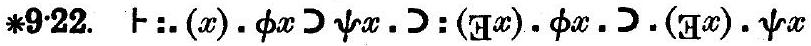
\includegraphics[max width=\textwidth, alt={}, center]{bc1848bf-39e8-4760-b069-9936044df683-008_46_811_1029_206}\\
I．e．if $\phi x$ always implies $\psi x$ ，then if $\phi x$ is sometimes true，so is $\psi x$ ．This proposition，like $* 9 \cdot 21$ ，is constantly used in the sequel．

Dem．\\
ト：$* 2: 08$ ．ɔํ：$\phi y$ つ $\psi y$. ɔ．$\phi y$ つ $\psi y$

ト．（1）．＊9．1．ɔト：（ $\mathrm{G}^{z}$ ）：$\phi y$ つ $\psi y$ ．ɔ．$\phi y$ つ $\psi z$

ト．（2）．＊91．ɔト：．$\left(\mathrm{H}^{x}\right): .(\mathrm{H} z): \phi x \supset \psi x . \supset . \phi y \supset \psi z$

ト．（3）．＊9．13．ɔ ：：$(y)::(\mathbb{H} x): .(\mathbb{H} z): \phi x \supset \psi x . \supset: \phi y \supset \psi z$\\
［（4）．（＊9．06）］$\quad \vdash::(y)::\left(\mathrm{G}^{x}\right): . \phi x \supset \psi x . \supset:\left(\mathrm{H}^{z}\right) . \phi y \supset \psi z$


\begin{equation*}
[(5) \cdot(* 1 \cdot 01 \cdot * 9 \cdot 08)] \quad \vdash::\left(\mathrm{G}^{x}\right) \cdot \sim(\phi x \supset \psi x): \mathrm{v}:(y):\left(\mathrm{H}^{z}\right) \cdot \phi y \supset \psi z \tag{5}
\end{equation*}



\begin{equation*}
[(6) .(* 1.01 . * 9.07)] \quad \vdash::(\mathrm{H} x) . \sim(\phi x \supset \psi x): \mathrm{v}:(y) . \sim \phi y . \mathrm{v} .(\mathrm{H} z) . \psi z \tag{6}
\end{equation*}



\begin{equation*}
[(7) .(* 1.01 . * 9.01 .02)] \vdash: .(x) . \phi x \supset \psi x . \supset:(\mathrm{H} y) . \phi y . \supset .(\mathrm{Hz}) . \psi z \tag{7}
\end{equation*}


This is the proposition to be proved，because（ $\mathrm{H} y$ ）．$\phi y$ is the same pro－ position as $\left(\mathrm{H}^{x}\right) \cdot \phi x$ ，and $\left(\mathrm{H}^{z}\right) \cdot \psi z$ is the same proposition as $\left(\mathrm{H}^{x}\right) \cdot \psi x$ ．\\
＊9．23．$\vdash:(x) . \phi x$. ɔ．$(x) . \phi x \quad$［Id．＊9．13．21］\\
＊9．24． ト：$\left(\mathrm{H}^{x}\right) . \phi x$. つ．$(\mathrm{H} x) . \phi x$［Id．＊9．13．22］\\
＊925． ト：．$(x) . p \vee \phi x$. つ：$p . v .(x) . \phi x$［＊9．23．（＊9．04）］\\
We are now in a position to prove the analogues of $* 1 \cdot 2-6$ ，replacing one of the letters $p, q, r$ in those propositions by $(x) \cdot \phi x$ or $(\mathbb{H} x) \cdot \phi x$ ．The proofs are given below．\\
＊9．3．$\vdash:(x) \cdot \phi x \cdot v \cdot(x) \cdot \phi x:$ J．$(x) \cdot \phi x$\\
Dem．\\
ト．＊1．2．ɔト．$\phi x \mathbf{v} \phi x$. ɔ．$\phi x$

ト．（1）．＊9．1．ɔト：（马y）：$\phi x \mathbf{v} \phi y$. ɔ．$\phi x$

ト．（2）．＊9．13．ɔํ：（ $x$ ）：．（马y $y$ ）：$\phi x$ v $\phi y$ ．ɔ．$\phi x$\\
［（3）．（＊9．05．01．04）］F：．（x）：．$\phi x . \mathrm{v} .(y) . \phi y:$ ɔ．$\phi x$

ト．（4）．＊9．21．ɔト：．$(x): \phi x . \mathrm{v} .(y) . \phi y:$ ɔ．$(x) . \phi x$\\
$[(5) \cdot(* 9 \cdot 03)] \quad \vdash: .(x) \cdot \phi x \cdot v \cdot(y) \cdot \phi y: \supset \cdot(x) \cdot \phi x:$ ɔ ⋅ ⋅ Prop\\
＊931． ト：$(G x)$ ．$\phi$ x．v．$(G x)$ ．$\phi x$ ：J．$(G x)$ ．$\phi x$\\
This is the only proposition which employs $* 911$ ．\\
Dem．


\begin{align*}
& \vdash \cdot * 9 \cdot 11 \cdot 13 . \quad \supset \vdash:(y): \phi x \vee \phi y \cdot \supset \cdot\left(\mathrm{H}^{z}\right) \cdot \phi z  \tag{1}\\
& {[(1) \cdot(* 9 \cdot 03 \cdot 02)] \quad \vdash:(\mathrm{H} y) \cdot \phi x \vee \phi y \cdot \supset \cdot\left(\mathrm{H}^{z}\right) \cdot \phi z}  \tag{2}\\
& \vdash \cdot(2) \cdot * 9 \cdot 13 \cdot \supset \vdash:(x):(\mathrm{H} y) \cdot \phi x \vee \phi y \cdot \supset \cdot(\mathrm{~Hz}) \cdot \phi z  \tag{3}\\
& {[(3) \cdot(* 9 \cdot 03 \cdot 02)] \quad \vdash: \cdot(\mathrm{H} x):(\mathrm{H} y) \cdot \phi x \vee \phi y: \supset \cdot(\mathrm{Hz}) \cdot \phi z}  \tag{4}\\
& {[(4) \cdot(* 9 \cdot 05 \cdot 06)] \quad \vdash:(\mathrm{H} x) \cdot \phi x \cdot \vee \cdot(\mathrm{H} y) \cdot \phi y: \supset \cdot(\mathrm{Hz}) \cdot \phi z}
\end{align*}


＊9．32． ！：$q$ ． ．$:(x)$ ．$\phi x$ ．$v$ ．$q$\\
Dem．

\[
\begin{array}{lr}
\vdash \cdot * 1 \cdot 3 . & \supset \vdash: q \cdot \supset: \phi x \cdot v \cdot q \\
\vdash \cdot(1) \cdot * 9 \cdot 13 . & \supset \vdash: .(x): q \cdot \supset: \phi x \cdot v \cdot q \\
{[* 9 \cdot 25]} & \supset \vdash:, q \cdot \supset:(x): \phi x \cdot v \cdot q  \tag{2}\\
{[(2) \cdot(* 9 \cdot 03)]} & \text { । }: q \cdot \supset:(x) \cdot \phi x \cdot \hat{v} \cdot q
\end{array}
\]

＊9．33．$F: q . \supset:\left(\mathrm{H}^{x}\right) . \phi x . \mathrm{v} . q$［Proof as above］\\
＊9．34．$\vdash:(x) . \phi x . \supset: p . \mathrm{v} .(x) . \phi x$\\
Dem．

\[
\begin{array}{ll}
\vdash . * 13 . & \supset \vdash: \phi x . \supset . p \vee \phi x \\
\vdash .(1) . * 9 \cdot 13 . & \supset \vdash:(x): \phi x . \supset . p \vee \phi x \\
\vdash .(2) . * 9 \cdot 21 . & \supset \vdash:(x) . \phi x . \supset .(x) . p \vee \phi x  \tag{3}\\
\text { ।.(3). }(* 9 \cdot 04) . \supset \vdash . \text { Prop }
\end{array}
\]

＊935．$F:\left(\mathrm{H}^{x}\right) . \phi x . \mathrm{J}: p . \mathrm{v} .\left(\mathrm{H}^{x}\right) . \phi x$［Proof as above］\\
＊9．36．$\vdash:, p . \mathrm{v} .(x) . \phi x:$ J ：$(x) . \phi x . \mathrm{v} . p$\\
Dem．

\[
\begin{array}{ll}
\vdash \cdot * 1 \cdot 4 . & \supset \vdash: p \vee \phi x \cdot \supset \cdot \phi x \vee p \\
\vdash \cdot(1) \cdot * 9 \cdot 13 \cdot 21 . & \supset \vdash:(x) \cdot p \vee \phi x \cdot \supset \cdot(x) \cdot \phi x \vee p  \tag{2}\\
\vdash .(2) \cdot(* 9 \cdot 03 \cdot 04) \cdot \supset \vdash . \text { Prop }
\end{array}
\]

＊9．361． ᄀ ：$(x) \cdot \phi x \cdot \mathrm{v} \cdot p:$ J ：$p \cdot \mathrm{v} \cdot(x) \cdot \phi x \quad$［Similar proof］\\
＊937． $\mathrm{F}:, p . \mathrm{v} .(\mathrm{H} x) . \phi x: \supset:(\mathrm{H} x) . \phi x . \mathrm{v} . p$［Similar proof］\\
＊9371．$\vdash:(\mathrm{H} x) . \phi x . \mathrm{v} . p:$ J：$p . \mathrm{v} .(\mathrm{H} x) . \phi x$［Similar proof］\\
＊94．$f:: p: \mathrm{v}: q \cdot \mathrm{v} \cdot(x) \cdot \phi x:$, J：$q: \mathrm{v}: p \cdot \mathrm{v} \cdot(x) \cdot \phi x$\\
Dem．


\begin{align*}
& \vdash \cdot * 1 \cdot 5 \cdot * 9 \cdot 21 \cdot \supset \vdash:(x): p \cdot v \cdot q \vee \phi x: \supset:(x): q \cdot v \cdot p \vee \phi x  \tag{1}\\
& \vdash \cdot(1) \cdot(* 9 \cdot 04) \cdot \supset \vdash \text {. Prop }
\end{align*}


＊9．401．$+: p: \mathrm{v}: q . \mathrm{v}$ ．（H $x$ ）．$\phi x:$ ．$: . q: \mathrm{v}: p . \mathrm{v}$ ．（ $\mathrm{H}^{x}$ ）．$\phi x$［As above］\\
＊941．F：：$p: \mathrm{v}:(x) . \phi x . \mathrm{v} . r: . \supset: .(x) . \phi x: \mathrm{v}: p \mathrm{v} r \quad$［As above］\\
＊9411．$\vdash:: p: \mathrm{v}:(\mathrm{H} x) \cdot \phi x \cdot \mathrm{v} \cdot r: . \mathrm{J}:,(\mathrm{G} x) \cdot \phi x: \mathrm{v}: p \mathrm{v} r$［As above］\\
＊942．$F::(x), \phi x: \mathrm{v}: q \vee r: . \mathrm{P}:, q: \mathrm{v}:(x), \phi x, \mathrm{v}, r \quad$［As above］\\
＊9421．$+::\left(\mathrm{G}^{x}\right) \cdot \phi x: \mathrm{v}: q \vee r: . \supset: q: \mathrm{v}:\left(\mathrm{H}^{x}\right) \cdot \phi x . \mathrm{v} \cdot r \quad$［As above］\\
＊9．5． ト ：$: p$ つ $q$ ．ɔ ：$p$ ．v．$(x)$ ．$\phi x:$ ɔ ：$q$ ．v．$(x)$ ．$\phi x$\\
Dem．\\
ト．＊1．6．ɔト：$p \supset q . \supset: p \vee \phi y . \supset . q \vee \phi y$

ト．（1）．$* 9 \cdot 1 \cdot(* 9 \cdot 06)$ ．วト：$p \supset q \cdot \supset:(\mathbb{H} x): p \vee \phi x . \supset \cdot q \vee \phi y$

ト．（2）．＊9．13．（＊9．04）．ɔㅐ：：$p \supset q . \supset: .(y): .\left(\mathrm{H}^{x}\right): p \vee \phi x . \supset . q \vee \phi y$\\
［（3）．（＊9．08）］$\quad \vdash:: p \supset q . \supset:(\mathbb{H} x) . \sim(p \vee \phi x) . \mathbf{v} .(y) . q \mathbf{v} \phi$\\
［（4）．（＊9．01）］$\quad \vdash:: p \supset q . \supset: .(x) . p \vee \phi x . \supset .(y) . q \vee \phi y$\\
［（5）．（＊9．04）］$\quad \vdash:: p \supset q . \supset:, p . \mathrm{v} .(x) . \phi x: \supset: q . \mathrm{v} .(y) . \phi y$\\
＊9501．$+:: p \supset q . \supset: p . \mathrm{v} .(\mathrm{H} x) . \phi x: \supset: q . \mathrm{v} .(\mathrm{H} x) . \phi x$［As above］\\
＊9：51．$\vdash:: p$. ɔ．$(x) . \phi x:$ ɔ ：$p \vee r$. つ：$(x) . \phi x . \vee . r$\\
Dem．

\[
\begin{array}{ll}
\vdash . * 16 . & \supset \vdash:, p \supset \phi x . \supset: p \vee r . \supset . \phi x \vee r \\
\vdash .(1) . * 9 \cdot 13 \cdot 21 . & \supset \vdash::(x) . p \supset \phi x . \supset:-(x): p \vee r . \supset . \phi x v r  \tag{2}\\
\vdash .(2) .(* 9.03 \cdot 04) . \supset \vdash . \operatorname{Prop} &
\end{array}
\]

＊9511．$\vdash:: p . \supset .(\mathrm{G} x) . \phi x: \supset: . p \vee r . \supset:\left(\mathrm{H}^{x}\right) . \phi x . \vee . r$［As above］\\
＊9：52．$\vdash::(x) \cdot \phi x \cdot \supset \cdot q: \supset: .(x) \cdot \phi x \cdot v \cdot r: \supset \cdot q \vee r$\\
Dem．

\[
\begin{array}{ll}
\vdash \cdot * 16 . & \supset \vdash: \phi x \supset q \cdot \supset: \phi x \vee r \cdot \supset \cdot q \vee r \\
\vdash \cdot(1) \cdot * 9 \cdot 13 \cdot 22 . & \supset \vdash::(\mathrm{H} x) \cdot \phi x \supset q \cdot \supset:(\mathrm{H} x): \phi x \vee r \cdot \supset \cdot q \vee r \\
\vdash \cdot(2) \cdot(* 9 \cdot 05 \cdot 01) \cdot \supset \vdash::(x) \cdot \phi x \cdot \supset \cdot q: \supset:(x) \cdot \phi x \vee r \cdot \supset \cdot q \vee r  \tag{3}\\
\text { 卜.(3).(*9.03). } & \supset \vdash . \text { Prop }
\end{array}
\]

＊9521．$\vdash::(\underset{\sim}{\eta} x) \cdot \phi x \cdot \supset \cdot q: \supset:\left(H^{x}\right) \cdot \phi x \cdot v \cdot r: \supset \cdot q \vee r$［As above］ ＊9．6．$(x) \cdot \phi x ; \sim(x) \cdot \phi x$ ，$\left(H^{x}\right) \cdot \phi x$ and $\sim\left(H^{x}\right) \cdot \phi x$ are of the same type．\\
［ $* 9 \cdot 131$ ，（7）and（8）］\\
＊9．61．If $\phi \hat{x}$ and $\psi \hat{x}$ are elementary functions of the same type，there is a function $\phi \hat{x} \mathbf{v} \psi \hat{x}$ ．

Dem．\\
By $* 9 \cdot 14 \cdot 15$ ，there is an $a$ for which＂$\psi a$ ，＂and therefore＂$\phi a$ ，＂are significant，and therefore so is＂$\phi a \mathbf{v} \psi a$ ，＂by the primitive idea of disjunction． Hence the result by $* 9 \cdot 15$ ．

The same proof holds for functions of any number of variables．\\
*9.62. If $\phi(\hat{x}, \hat{y})$ and $\psi \hat{z}$ are elementary functions, and the $x$-argument to $\phi$ is of the same type as the argument to $\psi$, there are functions

$$
(y) \cdot \phi(\hat{x}, y) \cdot v \cdot \psi \hat{x},(y y) \cdot \phi(\hat{x}, y) \cdot v \cdot \psi \hat{x} .
$$

Dem.\\
By *9•15, there are propositions $\phi(x, b)$ and $\psi a$, where by hypothesis $x$ and $a$ are of the same type. Hence by $* 9 \cdot 14$ there is a proposition $\phi(a, b)$, and therefore, by the primitive idea of disjunction, there is a proposition $\phi(a, b) \vee \psi a$, and therefore, by $* 9 \cdot 15$ and $* 9 \cdot 03$, there is a proposition $(y) \cdot \phi(a, y) \cdot \mathrm{v} \cdot \psi a$. Similarly there is a proposition (Hy) . $\phi(a, y) \cdot \mathrm{v} \cdot \psi a$. Hence the result, by $* 9.15$.\\
*9.63. If $\phi(\hat{x}, \hat{y}), \psi(\hat{x}, \hat{y})$ are elementary functions of the same type, there are functions $(y) \cdot \phi(\hat{x}, y) \cdot \mathrm{v} \cdot(z) \cdot \psi(\hat{x}, z)$, etc. [Proof as above]

We have now completed the proof that, in the primitive propositions of *1, any one of the propositions that occur may be replaced by $(x) \cdot \phi x$ or $(G x) . \phi x$. It follows that, by merely repeating the proofs, we can show that any other of the propositions that occur in these propositions can be simultaneously replaced by $(x) \cdot \psi x$ or $(H x) \cdot \psi x$. Thus all the primitive propositions of $* 1$, and therefore all the propositions of $* 2-* 5$, hold equally when some or all of the propositions concerned are of one of the forms (x) $\cdot \phi x$, ( $\mathrm{H} x$ ) $\cdot \phi x$, which was to be proved.

It follows, by mere repetition of the proofs, that the propositions of $* 1 — * 5$ hold when $p, q, r$ are replaced by propositions containing any number of apparent variables.

\section*{*10. THEORY OF PROPOSITIONS CONTAINING ONE APPARENT VARIABLE}
\section*{Summary of *10.}
The chief purpose of the propositions of this number is to extend to formal implications (i.e. to propositions of the form $(x) \cdot \phi x \supset \psi x$ ) as many as possible of the propositions proved previously for material implications, i.e. for propositions of the form $p \supset q$. Thus e.g. we have proved in *3.33 that

$$
\text { Put } \quad \begin{aligned}
& p \supset q \cdot q \supset r \cdot \supset \cdot p \supset r . \\
& p=\text { Socrates is a Greek }, \\
& q=\text { Socrates is a man, } \\
& r=\text { Socrates is a mortal. }
\end{aligned}
$$

Then we have " if 'Socrates is a Greek' implies 'Socrates is a man,' and 'Socrates is a man' implies 'Socrates is a mortal,' it follows that 'Socrates is a Greek' implies 'Socrates is a mortal.'" But this does not of itself prove that if all Greeks are men, and all men are mortals, then all Greeks are mortals.

Putting

$$
\begin{aligned}
& \phi x .=x \text { is a Greek, } \\
& \psi x .=x \text { is a man, } \\
& \chi^{x .}=x \text { is a mortal, }
\end{aligned}
$$

we have to prove

$$
(x) \cdot \phi x \supset \psi x:(x) \cdot \psi x \supset \chi x: \supset:(x) \cdot \phi x \supset \chi x .
$$

It is such propositions that have to be proved in the present number. It will be seen that formal implication $((x) \cdot \phi x \supset \psi x)$ is a relation of two functions $\phi \hat{x}$ and $\psi \hat{x}$. Many of the formal properties of this relation are analogous to properties of the relation " $p \supset q$ " which expresses material implication; it is such analogues that are to be proved in this number.

We shall assume in this number, what has been proved in $* 9$, that the propositions of *1-*5 can be applied to such propositions as $(x) \cdot \phi x$ and $\left(H^{x}\right) \cdot \phi x$. Instead of the method adopted in $* 9$, it is possible to take negation and disjunction as new primitive ideas, as applied to propositions containing apparent variables, and to assume that, with the new meanings of negation and disjunction, the primitive propositions of $* 1$ still hold. If this method is adopted, we need not take $(\pi x) \cdot \phi x$ as a primitive idea, but may put *10.01. ( $\mathrm{H} x) \cdot \phi x .=\sim \sim(x) \cdot \sim \phi x$ Df

In order to make it clear how this alternative method can be developed, we shall, in the present number, assume nothing of what has been proved in *9 except certain propositions which, in the alternative method, will be primitive propositions, and (what in part characterizes the alternative method)\\
the applicability to propositions containing apparent variables of analogues of the primitive ideas and propositions of $* 1$ ，and therefore of their conse－ quences as set forth in $* 2-* 5$ ．

The two following definitions merely serve to introduce a notation which is often more convenient than the notation $(x) \cdot \phi x \supset \psi x$ or $(x) \cdot \phi x \equiv \psi x$ ．\\
＊10．02．$\phi x \partial_{x} \psi x .=.(x) . \phi x \supset \psi x$ Df\\
＊10．03．$\phi x \equiv_{x} \psi x .=.(x) . \phi x \equiv \psi x$ ．Df\\
The first of these notations is due to Peano，who，however，has no notation for $(x) \cdot \phi x$ except in the special case of a formal implication．

The following propositions（＊10．1．11．12．121．122）have already been given in $* 9 . * 10.1$ is $* 9.2, * 10.11$ is $* 9.13, * 10.12$ is $* 9.25, * 10.121$ is $* 9.14$ ，and $* 10.122$ is $* 9.15$ ．These five propositions must all be taken as primitive propositions in the alternative method；on the other hand，$* 9.1$ and $* 9.11$ are not required as primitive propositions in the alternative method．

The propositions of the present number are very much used throughout the rest of the work．The propositions most used are the following：\\
＊101． $\mathrm{F}:(x) . \phi x$. ɔ．$\phi y$\\
I．e．what is true in all cases is true in any one case．\\
＊10．11．If $\phi y$ is true whatever possible argument $y$ may be，then $(x) \cdot \phi x$ is true．In other words，whenever the propositional function $\phi y$ can be asserted， so can the proposition $(x) \cdot \phi x$ ．\\
＊1021．F：．$(x) \cdot p \supset \phi x . \equiv: p . \supset .(x) . \phi x$\\
＊1022．$\vdash: .(x) \cdot \phi x \cdot \psi x . \equiv:(x) \cdot \phi x:(x) \cdot \psi x$\\
The conditions of significance in this proposition demand that $\phi$ and $\psi$ should take arguments of the same type．\\
＊10．23．$\vdash: .(x) . \phi x \supset p . \equiv:(\mathbb{H} x) . \phi x . \supset . p$\\
I．e．if $\phi x$ always implies $p$ ，then if $\phi x$ is ever true，$p$ is true．\\
＊10．24． ト：$\phi y$ ．ɔ ．$(\mathrm{H} x) \cdot \phi x$\\
I．e．if $\phi y$ is true，then there is an $x$ for which $\phi x$ is true．This is the sole method of proving existence－theorems．\\
＊10．27．$\vdash: .(z) . \phi z \supset \psi z . \supset:(z) . \phi z . \supset .(z) . \psi z$\\
I．e．if $\phi z$ always implies $\psi z$ ，then＂$\phi z$ always＂implies＂$\psi z$ always．＂The three following propositions，which are equally useful，are analogous to $* 10.27$ ．

\begin{verbatim}
*10.271.F:.(z). \phiz 引 \psiz. . : (z). \phiz. . .(z). ψz
*10.28. ':.(x).\phix ɔ \psix.):(Hx).\phix. . (Hx). \psix
*10281. +:.(x). \phix = ψx. ):(Hx). \phix.\Xi.(Hx). ψx
*1035. +:.(Hx).p.\phix.\equiv:p:(Hx).\phix
*10.42. ।:.(边). }\phix.\vee.(Hx). \psix:\equiv.(Hx). \phix v \psi
*105. F:.(Hx).\phix.\psix.):(Hx).\phix:(Hx).\psix
\end{verbatim}

It should be noticed that whereas $* 10.42$ expresses an equivalence, $* 10.5$ only expresses an implication. This is the source of many subsequent differences between formulae concerning addition and formulae concerning multiplication.\\
*10.51. $\vdash: \sim \sim\left\{\left(\mathrm{H}^{x}\right), \phi x, \psi x\right\} . \equiv \phi x . \nu_{x} \sim \psi x$\\
This proposition is analogous to

$$
\vdash: \sim(p \cdot q) \cdot \equiv p \supset \sim q
$$

which results from *4.63 by transposition.\\
Of the remaining propositions of this number, some are employed fairly often, while others are lemmas which are used only once or twice, sometimes at a much later stage.\\
*10.01. (G $x$ ). $\phi x .=. \sim(x) . \sim \phi x$ Df\\
This definition is only to be used when we discard the method of $* 9$ in favour of the alternative method already explained. In either case we have

$$
\vdash:(\pi x) \cdot \phi x \equiv \equiv \sim(x) \cdot \sim \phi x .
$$

*10.02. $\phi x \supset_{x} \psi x=(x) \cdot \phi x \supset \psi x$ Df\\
*10.03. $\phi x \equiv_{x} \psi x .=.(x) . \phi x \equiv \psi x$ Df\\
*10-1. $\mathrm{F}:(x) . \phi x$. J. $\phi y$ [*9.2]\\
*10.11. If $\phi y$ is true whatever possible argument $y$ may be, then $(x) \cdot \phi x$ is true. [*9-13]

This proposition is, in a sense, the converse of $* 10 \cdot 1 . * 10 \cdot 1$ may be stated: "What is true of all is true of any," while *10-11 may be stated: "What is true of any, however chosen, is true of all."\\
*10-12. + : $(x) . p \vee \phi a$. D: $p . v .(x) . \phi x[* 9.25]$\\
According to the definitions in $\boldsymbol{*} \mathbf{9}$, this proposition is a mere example of " $q \supset q$," since by definition the two sides of the implication are different symbols for the same proposition. According to the alternative method, on the contrary, $* 10 \cdot 12$ is a substantial proposition.\\
*10121. If " $\phi x$ " is significant, then if $a$ is of the same type as $x$, " $\phi a$ " is significant, and vice versa. [*9:14]

It follows from this proposition that two arguments to the same function must be of the same type ; for if $x$ and $a$ are arguments to $\phi \hat{x}$, " $\phi x$ " and " $\phi a$ " are significant, and therefore $x$ and $a$ are of the same type. Thus the above primitive proposition embodies the outcome of our discussion of the viciouscircle paradoxes in Chapter II of the Introduction.\\
*10.122. If, for some $a$, there is a proposition $\phi a$, then there is a function $\phi \hat{x}$, and vice versa. [*9-15]\\
*1013. If $\phi \hat{x}$ and $\psi \hat{x}$ take arguments of the same type, and we have " $+\phi x$ " and " $\vdash . \psi x$," we shall have " $\vdash . \phi x . \psi x$."

Dem．\\
By repeated use of $* 9 \cdot 61 \cdot 62 \cdot 63 \cdot 131(3)$ ，there is a function $\sim \dot{\phi} \hat{x} \mathbf{v} \sim \psi \hat{x}$ ． Hence by $* 2 \cdot 11$ and $* 3 \cdot 01$ ，


\begin{align*}
& \vdash: \sim \phi x \mathbf{v} \sim \psi x \cdot \mathbf{v} \cdot \phi x \cdot \psi x  \tag{1}\\
& \vdash \cdot(1) \cdot * 2 \cdot 32 \cdot(* 1 \cdot 01) \cdot \supset \vdash:, \phi x \cdot \supset: \psi x \cdot \supset \cdot \phi x \cdot \psi x  \tag{2}\\
& \vdash \cdot(2) \cdot * 9 \cdot 12 \cdot \supset+. \text { Prop }
\end{align*}


＊10－14．$\vdash: .(x) \cdot \phi x:(x) \cdot \psi x: \supset \cdot \phi y \cdot \psi y$\\
This proposition is true whenever it is significant，but it－is not always significant when its hypothesis is significant．For the thesis demands that $\phi$ and $\psi$ should take arguments of the same type，while the hypothesis does not demand this．Hence，if it is to be applied when $\phi$ and $\psi$ are given，or when $\psi$ is given as a function of $\phi$ or vice versa，we must not argue from the hypothesis to the thesis unless，in the supposed case，$\phi$ and $\psi$ take arguments of the same type．

Dem．

\[
\begin{array}{ll}
\vdash \cdot * 10 \cdot 1 . & \supset \vdash:(x) \cdot \phi x \cdot \supset \cdot \phi y \\
\vdash \cdot * 10 \cdot 1 . & \supset \vdash:(x) \cdot \psi x \cdot \supset \cdot \psi y  \tag{2}\\
\vdash \cdot(1) \cdot(2) \cdot * 10 \cdot 13 \cdot \supset f:(x) \cdot \phi x \cdot \supset \cdot \phi y:(x) \cdot \psi x \cdot \supset \cdot \psi y: \\
{[* 3 \cdot 47] \quad \cdot \quad \supset \vdash:(x) \cdot \phi x:(x) \cdot \psi x: \supset \cdot \phi y \cdot \psi y: . \supset \vdash \cdot \text { Prop }} \\
* 10 \cdot 2 . \quad \vdash: .(x) \cdot p \vee \phi x \cdot \equiv: p \cdot v \cdot(x) \cdot \phi x
\end{array}
\]

Dem．

\[
\begin{array}{ll}
\vdash \cdot * 10 \cdot 1 \cdot * 1 \cdot 6 \cdot & \supset \vdash: p \cdot v \cdot(x) \cdot \phi x: \supset \cdot p \vee \phi y: . \\
{[* 10 \cdot 11]} & \supset \vdash: \cdot(y): p \cdot v \cdot(x) \cdot \phi x: \supset \cdot p \vee \phi y: . \\
{[* 10 \cdot 12]} & \supset \vdash: \cdot p \cdot v \cdot(x) \cdot \phi x: \supset \cdot(y) \cdot p \vee \phi y \\
\vdash \cdot * 10 \cdot 12 . & \supset \vdash: \cdot(y) \cdot p v \phi y \cdot \supset: p \cdot v \cdot(x) \cdot \phi x  \tag{2}\\
\vdash \cdot(1) \cdot(2) . & \supset \vdash . \text { Prop }
\end{array}
\]

＊10．21．$\vdash:(x) \cdot p \supset \phi x . \equiv: p . \supset .(x) . \phi x\left[* 10.2 \frac{\sim p}{p}\right]$\\
This proposition is much more used than $* 10.2$ ．\\
＊10．22．$\vdash: .(x) \cdot \phi x \cdot \psi x \cdot \equiv:(x) \cdot \phi x:(x) \cdot \psi x$\\
Dem．


\begin{align*}
& \text { ト.*101. ɔト: }(x) . \phi x . \psi x . \text { ɔ. } \phi y . \psi y .  \tag{1}\\
& \text { [*326] ɔ.φy: } \\
& \text { [*10.11] ɔト: }(y):(x) \cdot \phi x \cdot \psi x \cdot \supset \cdot \phi y: . \\
& \text { [*10.21] ɔ.t:. }(x) . \phi x . \psi x . \supset .(y) . \phi y  \tag{2}\\
& \text { ト. (1). *3.27. ɔํ:. (x). } \phi x \text {. } \psi x \text {. ɔ. } \psi z \text { : } \\
& \text { [*10.11] ɔト:. }(z):(x) . \phi x . \psi x . \supset . \psi z: . \\
& \text { [*10.21] ɔト:.(x). } \phi x . \psi x . \supset .(z) . \psi z  \tag{3}\\
& \text { ト.(2).(3).Comp.ɔㄴ:. (x). } \phi x \cdot \psi x \cdot \supset:(y) \cdot \phi y:(z) \cdot \psi z  \tag{4}\\
& \text { ト. } * 10 \text { 14-11. } \quad \supset \vdash:(y): .(x) \cdot \phi x:(x) \cdot \psi x: \supset \cdot \phi y \cdot \psi y: . \\
& \text { [*10.21] } \quad \supset+: .(x) . \phi x:(x) . \psi x: \supset .(y) . \phi y . \psi y  \tag{5}\\
& \text { ト.(4).(5). ɔト.Prop }
\end{align*}


The above proposition is true whenever it is significant; but, as was pointed out in connexion with $\boldsymbol{*} \mathbf{1 0} \cdot \mathbf{1 4}$, it is not always significant when $"(x) \cdot \phi x:(x) \cdot \psi x$ " is significant.\\
*10221. If $\phi x$ contains a constituent $\chi(x, y, z, \ldots)$ and $\psi x$ contains a constituent $\chi(x, u, v, \ldots)$, where $\chi$ is an elementary function and $y, z, \ldots u, v, \ldots$ are either constants or apparent variables, then $\phi \hat{x}$ and $\psi \hat{x}$ take arguments of the same type. This can be proved in each particular case, though not generally, provided that, in obtaining $\phi$ and $\psi$ from $\chi, \chi$ is only submitted to negations, disjunctions and generalizations. The process may be illustrated by an example. Suppose $\phi x$ is $(y) \cdot \chi(x, y) \cdot \supset \cdot \theta x$, and $\psi x$ is $f x \cdot \supset \cdot(y) \cdot \chi(x, y)$. By the definitions of $* 9, \phi x$ is $(\mathbb{H} y) \sim \chi(x, y) \vee \theta x$, and $\psi x$ is $(y) . \sim f x \vee \chi(x, y)$. Hence since the primitive ideas $(x) . F x$ and $\left(H^{x}\right) . F x$ only apply to functions, there are functions $\sim \chi(\hat{x}, \hat{y}) \vee \theta \hat{x}, \sim f \hat{x} \mathbf{v} \chi(\hat{x}, \hat{y})$. Hence there is a proposition $\sim \chi(a, b) \vee \theta a$. Hence, since " $p \vee q$ " and " $\sim p$ " are only significant when $p$ and $q$ are propositions, there is a proposition $\chi(a, b)$. Similarly, for some $u$ and $v$, there are propositions $\sim f u \vee \chi(u, v)$ and $\chi(u, v)$. Hence by $* 9 \cdot 14, u$ and $a, v$ and $b$ are respectively of the same type, and (again by $* 9 \cdot 14$ ) there is a proposition $\sim f a \vee \chi(a, b)$. Hence (*9•15) there are functions $\sim \chi(a, \hat{y}) \vee \theta a, \sim f a \vee \chi(a, \hat{y})$, and therefore there are propositions

$$
(G y) \sim \chi(a, y) \vee \theta a,(y) \sim \sim f a \vee \chi(a, y),
$$

i.e. there are propositions $\phi a, \psi a$, which was to be proved. This process can be applied similarly in any other instance.\\
*10.23. । : $(x) \cdot \phi x \supset p . \equiv:($ g $x) \cdot \phi x . \supset . p$\\
Dem.

\[
\begin{array}{lr}
\vdash \cdot * 4 \cdot 2 \cdot(* 9 \cdot 03) \cdot \supset \vdash:(x) \cdot \sim \phi x \vee p \cdot \equiv:(x) \cdot \sim \phi x \cdot \vee \cdot p: \\
\begin{aligned}
{[(* 9 \cdot 02)] } & \equiv \cdot(H x) \cdot \phi x \cdot \supset \cdot p \\
\vdash \cdot(1) \cdot(* 1 \cdot 01) \cdot \supset \vdash \cdot \text { Prop } &
\end{aligned} \tag{1}
\end{array}
\]

In the above proof, we employ the definitions of $* 9$. In the alternative method, in which ( $H x$ ). $\phi x$ is defined in accordance with $* 10.01$, the proof proceeds as follows.\\
*10.23. $\vdash: .(x) . \phi x \supset p . \equiv:(\mathrm{H} x) . \phi x . \supset . p$\\
Dem.

\[
\begin{array}{lr}
\vdash . \text { Transp } \cdot(* 10 \cdot 01) \cdot \supset \vdash:\left(H^{x}\right) \cdot \phi x \cdot \supset \cdot p: & \equiv: \sim p \cdot \supset \cdot(x) \cdot \sim \phi x: \\
\begin{array}{ll}
{[* 10 \cdot 21]} & \equiv:(x): \sim p \cdot \supset \cdot \sim \phi x: \\
{[* 10 \cdot 1]} & \supset: \sim p \cdot \supset \cdot \sim \phi x: \\
{[\text { Transp }]} & \supset: \phi x \cdot \supset \cdot p: . \\
{[* 10 \cdot 11]} & \supset \vdash:(x):\left(H^{x}\right) \cdot \phi x \cdot \supset \cdot p: \supset: \phi x \cdot \supset \cdot p: .
\end{array} \tag{1}
\end{array}
\]

$$
\begin{array}{ll}
{[* 10 \cdot 21]} & \supset \vdash:(\mathrm{H} x) \cdot \phi x \cdot \supset \cdot p: \supset:(x): \phi x \cdot \supset \cdot p \\
\vdash \cdot * 10 \cdot 1 & \supset F:(x): \phi x \cdot \supset \cdot p: \supset: \phi x \supset p: \\
{[\text { Transp }]} & \\
{[* 10 \cdot 11 \cdot 21]} & \supset F:(x): \phi x \cdot \supset \cdot p: \supset:(x): \sim p \cdot \supset \cdot \sim \phi x: \\
{[(1)]} & \supset:(\mathrm{H} x) \cdot \phi x \cdot \supset \cdot p
\end{array}
$$

ト．（2）．（3）．ɔト．Prop\\
Whenever we have an asserted proposition of the form $p \supset \phi x$ ，we can pass by $* 10 \cdot 11 \cdot 21$ to an asserted proposition $p . \supset .(x) . \phi x$ ．This passage is constantly required，as in the last line but one of the above proof．It will be indicated merely by the reference＂$* 10 \cdot 11 \cdot 21$ ，＂and the two steps which it requires will not be separately put down．\\
＊10．24． । ：$\phi y$ ．ɔ ．$(\mathbb{H} x) \cdot \phi x$\\
This is $* 9 \cdot 1$ ．In the alternative method，the proof is as follows．\\
Dem．

$$
\begin{aligned}
& \vdash . * 10 \cdot 1 . \supset \vdash:(x) . \sim \phi x . \supset . \sim \phi y: \\
& {[\text { Transp }] \text { つ }: \phi y . \supset . \sim(x) . \sim \phi x:} \\
& {[(* 10.01)] \supset \vdash . \text { Prop }}
\end{aligned}
$$

＊10．25．$\vdash:(x) . \phi x$. つ $.\left(\mathrm{H}^{x}\right) . \phi x$［＊10．124］\\
＊10．251．$f:(x) . \sim \phi x . \supset . \sim\{(x) . \phi x\}$［＊10．25．Transp］\\
＊10．252． $\mathrm{F}: \sim\left\{\left(\mathrm{H}^{x}\right) \cdot \phi x\right\} \cdot \equiv \cdot(x) \cdot \sim \phi x \quad[* 4 \cdot 2 .(* 9 \cdot 02)]$\\
＊10．253．$+: \sim\{(x) . \phi x\} . \equiv .(\mathbb{H} x) . \sim \phi x \quad[* 4.2 .(* 9.01)]$\\
In the alternative method，in which $(\mathcal{H} x) \cdot \phi x$ is defined as in $* 10 \cdot 01$ ，the proofs of $* 10 \cdot 252 \cdot 253$ are as follows．\\
＊10．252． $\mathrm{F}: \sim\{(\mathrm{H} x) \cdot \phi x\} \cdot \equiv .(x) \cdot \sim \phi x \quad[* 4 \cdot 13 .(* 10 \cdot 01)]$\\
＊10．253． $\mathrm{F}: \sim\{(x) \cdot \phi x\} \cdot \equiv \cdot(\mathrm{H} x) \cdot \sim \phi x$\\
Dem．


\begin{align*}
& \text { ト. } * 10 \text {.1. ɔ : }(x) \text {. } \phi x \text {. ɔ. } \phi y \text {. } \\
& \text { [*2•12] ɔ~~(~φy): } \\
& \text { [*10.11.21] ว! : }(x) . \phi x . \supset .(y) . \sim(\sim \phi y): \\
& \text { [Transp] ɔ : : } \sim\{(y) . \sim(\sim \phi y)\} . \supset . \sim\{(x) . \phi x\}: \\
& \text { [(*10.01)] ɔㅏ:(Hy).~φy. ɔ.~\{(x).φx\} }  \tag{1}\\
& \text { ৮. } * 101 \text {. ɔト: }(y) \sim(\sim \phi y) \text {. ɔ.~ (~φx). } \\
& \text { [*2:14] ɔ.φx: } \\
& \text { [*10.11•21]ɔา: }(y) . \sim(\sim \phi y) . \quad \text { ɔ. }(x) . \phi x: \\
& \text { [Transp] ɔ : } \sim\{(x) \cdot \phi x\} \text {. ɔ . } \sim\{(y) . \sim(\sim \phi y)\} \text {. } \\
& \text { [(*10.01)] ɔ.(廿y).~φy }  \tag{2}\\
& \text { ト.(1).(2).ɔ }
\end{align*}


＊10．26．$F: .(z) . \phi z \supset \psi z: \phi x:$ D．$\psi x$［＊10．1．Imp］\\
This is one form of the syllogism in Barbara．E．g．put $\phi z .=. z$ is a man， $\psi z .=. z$ is mortal，$x=$ Socrates．Then the proposition becomes：\\
＂If all men are mortal，and Socrates is a man，then Socrates is mortal．＂\\
Another form of the syllogism in Barbara is given in $* 103$ ．The two forms，formerly wrongly identified，were first distinguished by Peano and Frege．\\
＊1027．$\vdash: .(z) . \phi z \supset \psi z . \supset:(z) . \phi z . \supset .(z) . \psi z$\\
This is $* 9.21$ ．In the alternative method，the proof is as follows．\\
Dem．

\[
\begin{array}{lc}
\vdash \cdot * 10 \cdot 14 \cdot & \supset \vdash: \cdot(z) \cdot \phi z \supset \psi z:(z) \cdot \phi z: \supset \cdot \phi y \supset \psi y \cdot \phi y \cdot \\
& \supset \cdot \psi y: \\
{[\text { Ass }]} & \\
{[* 10 \cdot 1]} & \supset \vdash: \cdot(y): \cdot(z) \cdot \phi z \supset \psi z:(z) \cdot \phi z: \supset \cdot \psi y:  \tag{1}\\
{[* 10 \cdot 21]} & \supset \vdash: \cdot(z) \cdot \phi z \supset \psi z:(z) \cdot \phi z: \supset \cdot(y) \cdot \psi y \\
\vdash \cdot(1) \cdot \text { Exp } \cdot \text { ว } \vdash \cdot \text { Prop }
\end{array}
\]

＊10271．$\vdash: .(z) \cdot \phi z \equiv \psi z \cdot \omega:(z) \cdot \phi z \cdot \equiv \cdot(z) \cdot \psi z$\\
Dem．

\[
\begin{array}{lc}
\vdash \cdot * 10 \cdot 22 & \supset \vdash:, \mathrm{Hp} \cdot \supset:(z) \cdot \phi z \supset \psi z: \\
{[* 10 \cdot 27]} & \supset:(z) \cdot \phi z \cdot \supset \cdot(z) \cdot \psi z \\
\vdash \cdot * 10 \cdot 22 & \supset \vdash:, \mathrm{Hp} \cdot \supset:(z) \cdot \psi z \supset \phi z: \\
{[* 10 \cdot 27]} & \supset:(z) \cdot \psi z \cdot \supset \cdot(z) \cdot \phi z  \tag{2}\\
\vdash \cdot(1) \cdot(2) \cdot \text { Comp } \cdot \supset \vdash . \text { Prop }
\end{array}
\]

＊1028．$\vdash: .(x) \cdot \phi x \supset \psi x \cdot \supset:\left(\mathcal{H}^{x}\right) \cdot \phi x \cdot \supset \cdot(\mathrm{H} x) \cdot \psi x$\\
This is $* 9: 22$ ．In the alternative method，the proof is as follows．\\
Dem．\\
ト．＊101．ɔト：$(x) . \phi x$ つ $\psi x$. ɔ．$\phi y$ つ $\psi y$ ．\\
［Transp］ɔ．～ψy ɔ～φy：．\\
$[* 10 \cdot 11 \cdot 21]$ วト ：$(x) \cdot \phi x \supset \psi x . \supset:(y) \cdot \sim \psi y \supset \sim \phi y:$\\
［＊10．27］$\supset:(y) \sim \psi y . \supset .(y) . \sim \phi y:$\\
［Transp］ɔ：（马y）．$\phi y$ ．ɔ．（み $y), \psi y$ ：．ɔト．Prop\\
$* 10281$ ．$:(x) \cdot \phi x \equiv \psi x . \supset:\left(\mathrm{G}^{x}\right) \cdot \phi x . \equiv \cdot\left(\mathrm{G}^{x}\right) \cdot \psi x$［＊10．22＊28．Comp］\\
＊10．29．$\vdash:(x) \cdot \phi x \supset \psi x:(x) \cdot \phi x \supset \chi^{x}: \equiv:(x): \phi x . \supset \cdot \psi x . \chi^{x}$ ．\\
Dem．

\[
\begin{array}{cc}
\vdash \cdot * 10 \cdot 22 . & \supset \vdash:(x) \cdot \phi x \supset \psi x:(x) \cdot \phi x \supset \chi x: \\
& \equiv:(x): \phi x \supset \psi x \cdot \phi x \supset \chi^{x} \\
\vdash \cdot * 4 \cdot 76 . & \supset \vdash: \phi x \supset \psi x \cdot \phi x \supset \chi^{x} \cdot \equiv: \phi x \cdot \supset \cdot \psi x \cdot \chi^{x}: \\
{[* 10 \cdot 11] \quad \supset \vdash:(x): \phi x \supset \psi x \cdot \phi x \supset \chi^{x} \cdot \equiv: \phi x \cdot \nu \cdot \psi x \cdot \chi^{x}:} \\
{[* 10 \cdot 271] \quad \supset \vdash:(x): \phi x \supset \psi x \cdot \phi x \supset \chi^{x}: \equiv:(x): \phi x \cdot \supset \cdot \psi x \cdot \chi^{x}}  \tag{2}\\
\text { F.(1).(2). } \supset \vdash . \text { Prop }
\end{array}
\]

This is an extension of the principle of composition．\\
＊10．3．$\quad \vdash:(x) \cdot \phi x \supset \psi x:(x) \cdot \psi x \supset \chi x: \supset \cdot(x) \cdot \phi x \supset \chi x$\\
This is the second form of the syllogism in Barbara．\\
Dem．

$$
\begin{aligned}
& \vdash . * 10.22 \cdot 221 . \text { ɔ }: \text { Hp } . \text { ɔ } .(x) . \phi x \text { つ } \psi x . \psi x \text { つ } \chi^{x} . \\
& \text { [Syll. } * 10.27] \quad \text { ɔ } .(x) . \phi x \text { つ } \chi^{x}: \text { ɔ } \text {. Prop }
\end{aligned}
$$

＊10．301．$+:(x) \cdot \phi x \equiv \psi x:(x) \cdot \psi x \equiv \chi^{x}: \circlearrowright \cdot(x) \cdot \phi x \equiv \chi^{x}$\\
Dem．

$$
\begin{aligned}
\vdash \cdot * 10 \cdot 22 \cdot 221 . & \supset \vdash: \mathrm{Hp} \cdot \supset:(x) \cdot \phi x \equiv \psi x \cdot \psi x=\chi^{x}: \\
{[* 4 \cdot 22 \cdot * 10 \cdot 27] } & \supset:(x) \cdot \phi x \equiv \chi^{x}: . \supset \vdash \text {. Prop }
\end{aligned}
$$

In the second line of the proofs of $* 10.3$ and $* 10.301$ ，we abbreviate the process of proof in a way which is often convenient．In $* 10 \cdot 3$ ，the full process would be as follows：

$$
\begin{aligned}
& \vdash . \text { Syll. } \supset \vdash: \phi x \supset \psi x . \psi x \supset \chi x . \supset . \phi x \supset \chi x: \\
& {[* 10.11] \supset \vdash:(x): \phi x \supset \psi x . \psi x \supset \chi^{x} . \supset . \phi x \supset \chi x:} \\
& {[* 10.27] \supset \vdash:(x) \cdot \phi x \supset \psi x . \psi x \supset \chi^{x} . \supset .(x) . \phi x \supset \chi^{x}}
\end{aligned}
$$

The above two propositions show that formal implication and formal equivalence are transitive relations between functions．\\
＊10．31．$\vdash: .(x) . \phi x \supset \psi x . \supset:(x): \phi x . \chi x . \supset . \psi x . \chi^{x}$\\
Dem．


\begin{align*}
& \vdash . \text { Fact } . * 10 \cdot 11 . \supset \vdash: .(x): \phi x \supset \psi x . \supset: \phi x \cdot \chi x . \supset . \psi x . \chi^{x}  \tag{1}\\
& \vdash .(1) \cdot * 10 \cdot 27 . \supset \vee . \text { Prop }
\end{align*}


＊10．311．$\vdash: .(x) . \phi x \equiv \psi x.):(x): \phi x . \chi^{x} . \equiv . \psi x . \chi^{x}$\\
Dem．


\begin{align*}
& \vdash \cdot * 4 \cdot 36 \cdot * 10 \cdot 11 \cdot \supset \vdash:(x): . \phi x \equiv \psi x \cdot \supset: \phi x \cdot \chi^{x} \cdot \equiv: \psi x \cdot \chi^{x}  \tag{1}\\
& \vdash \cdot(1) \cdot * 10 \cdot 27 . \quad \supset \vdash . \text { Prop }
\end{align*}


The above two propositions are extensions of the principle of the factor．\\
＊10．32． $\mathrm{F}: \phi x \equiv_{x} \psi x . \equiv . \psi x \equiv_{x} \phi x$\\
Dem．

$$
\begin{aligned}
\vdash . * 10.22 . \supset \vdash: \phi x \equiv_{x} \psi x . & \equiv \phi x \supset_{x} \psi x . \psi x \supset_{x} \phi x . \\
{[* 4.3] } & \equiv \psi x \supset_{x} \phi x . \phi x \partial_{x} \psi x . \\
{[* 10.22] } & \equiv . \psi x \equiv_{x} \phi x: \supset \vdash . \text { Prop }
\end{aligned}
$$

This proposition shows that formal equivalence is symmetrical．\\
＊10．321．$\vdash: \phi x \equiv_{x} \psi x . \phi x \equiv_{x} \chi^{x}$ ．J．$\psi x \equiv_{x} \chi^{x}$\\
Dem．

$$
\begin{aligned}
& \text { 卜.*10.32. Fact. ɔ : Hp. ɔ . } \psi x \equiv_{x} \phi x . \phi x \equiv_{x} \chi^{x} . \\
& \text { [*10.301] } \text { ว. } \psi x \equiv_{x} \chi^{x}: \supset \vdash . \text { Prop }
\end{aligned}
$$

＊10．322．$\vdash: \psi x \equiv_{x} \phi x \cdot \chi^{x} \equiv_{x} \phi x \cdot$ J．$\psi x \equiv_{x} \chi^{x}$\\
Dem．

$$
\begin{aligned}
& \vdash . * 10.32 . \text { つ }: \text { Hp } . \text { ɔ } . \psi x \equiv_{x} \phi x . \phi x \equiv_{x} \chi^{x} . \\
& {[* 10.301] \text { つ. } \psi x \equiv_{x} \chi^{x}: \supset \vdash . \text { Prop }}
\end{aligned}
$$

*10.33. $\vdash: .(x): \phi x, p: \equiv:(x), \phi x: p$\\
Dem.

\[
\begin{array}{ll}
\vdash . * 10 \cdot 1 . & \supset \vdash: .(x): \phi x \cdot p: \supset \cdot \phi y \cdot p . \\
{[* 3 \cdot 27]} & \\
\vdash .(1) \cdot * 3 \cdot 26 . \supset \vdash:(x): \phi x \cdot p: \supset \cdot \phi y: \\
{[* 10 \cdot 11 \cdot 21]} & \supset \vdash: .(x): \phi x \cdot p: \supset \cdot(y) \cdot \phi y \\
\vdash .(2) \cdot(3) . & \supset \vdash:(x): \phi x \cdot p: \supset:(y) \cdot \phi y: p \\
\vdash \cdot * 10 \cdot 1 . & \supset \vdash:(y) \cdot \phi y . \quad \supset \cdot \phi x: . \\
{[\text { Fact }]} & \supset \vdash:(y) \cdot \phi y: p: \supset \cdot \phi x \cdot p: . \\
{[* 10 \cdot 11 \cdot 21]} & \supset \vdash: .(y) \cdot \phi y: p: \supset:(x): \phi x \cdot p  \tag{5}\\
\vdash .(4) \cdot(5) . & \supset \vdash . \text { Prop }
\end{array}
\]

*10.34. $\vdash:(\mathrm{G} x) \cdot \phi x \supset p \cdot \equiv:(x) \cdot \phi x \cdot \supset \cdot p$\\
This follows immediately from $* 9.05 .01$ and $* 1.01$. In the alternative method, the proof is as follows.

Dem.

$$
\begin{array}{ll}
\vdash \cdot * 4 \cdot 2 \cdot(* 10 \cdot 01) \cdot \supset & \\
\vdash: \cdot\left(H^{x}\right) \cdot \phi x \supset p . & \equiv: \sim\{(x) \cdot \sim(\phi x \supset p)\}: \\
{[* 4 \cdot 61 \cdot * 10 \cdot 271]} & \equiv: \sim\{(x): \phi x \cdot \sim p\}: \\
{[* 10 \cdot 33]} & \equiv: \sim\{(x) \cdot \phi x: \sim p\}: \\
{[* 4 \cdot 53]} & \equiv: \sim\{(x) \cdot \phi x\} \cdot v \cdot p: \\
{[* 4 \cdot 6]} & \equiv:(x) \cdot \phi x \cdot \supset \cdot p
\end{array}
$$

*1035. $\vdash: .(\mathrm{G} x) \cdot p \cdot \phi x . \equiv: p:(\mathrm{G} x) \cdot \phi x$\\
Dem.

\[
\begin{array}{ll}
\vdash \cdot * 3 \cdot 26 \cdot & \supset f: p \cdot \phi x \cdot \supset \cdot p: \\
{[* 10 \cdot 11]} & \supset f:(x): p \cdot \phi x \cdot \supset \cdot p: \\
{[* 10 \cdot 23]} & \supset f:(\mathrm{H} x) \cdot p \cdot \phi x \cdot \supset \cdot p \\
\vdash \cdot * 3 \cdot 27 \cdot & \supset f: p \cdot \phi x \cdot \supset \cdot \phi x: \\
{[* 10 \cdot 11]} & \supset f:(x): p \cdot \phi x \cdot \supset \cdot \phi x: \\
{[* 10 \cdot 28]} & \supset f:(\mathrm{H} x) \cdot p \cdot \phi x \cdot \supset \cdot(\mathrm{H} x) \cdot \phi x \\
f \cdot * 3 \cdot 2 \cdot & \supset f: p \cdot \supset: \phi x \cdot \supset \cdot p \cdot \phi x \cdot \\
{[* 10 \cdot 11 \cdot 21] \supset f: p \cdot \supset:(x): \phi x \cdot \supset \cdot p \cdot \phi x:} \\
{[* 10 \cdot 28]} & \supset:(\mathrm{H} x) \cdot \phi x \cdot \supset \cdot(\mathrm{H} x) \cdot p \cdot \phi x  \tag{3}\\
f \cdot(1) \cdot(2) \cdot(3) \cdot \text { Imp } \cdot \supset f \cdot \text { Prop }
\end{array}
\]

*1036. $\vdash: .(\mathbb{H} x) \cdot \phi x \vee p \cdot \equiv:(\mathbb{H} x) \cdot \phi x \cdot v \cdot p$\\
This follows immediately from $* 9.05$. In the alternative method, the proof is as follows.

Dem.

\begin{verbatim}
+.*4.64. \supsetト:\phixvp.\equiv.~\phix\supsetp:
[*10.11] \supset':(x):\phixvp.\equiv.~\phix\supsetp:
[*10.281] \supset':.(Hx).\phixvp.\equiv:(Hx).~\phix\supsetp:
[*10.34] \equiv:(x).~\phix.\supset.p:
[*4.6.(*10.01)] \equiv:(Hx).\phix.v.p:.\supset\vdash.Prop
\end{verbatim}

The above proposition is only required in order to lead to the following：\\
＊10．37． ト：$($ 月 $x) \cdot p \supset \phi x . \equiv: p . \supset$ ．（马 $x$ ）.$\phi x\left[* 10.36 \frac{\sim p}{p}\right]$\\
＊1039．$\vdash:, \phi x \supset_{x} \chi x: \psi x \partial_{x} \theta x: \supset: \phi x \cdot \psi x \cdot \partial_{x} \cdot \chi^{x} \cdot \theta x$\\
Dem．

$$
\begin{aligned}
& \vdash . * 10 \cdot 22 . \text { ɔ }: . \mathrm{Hp} . \supset:(x): \phi x \supset \chi x . \psi x \supset \theta x: \\
& {[* 3 \cdot 47 . * 10 \cdot 27] \quad \supset:(x): \phi x . \psi x . \supset . \chi^{x} . \theta x: . \supset \vdash . \text { Prop }}
\end{aligned}
$$

This proposition is only true when the conclusion is significant；the significance of the hypothesis does not insure that of the conclusion．On the conditions of significance，see the remarks on $* 10 \cdot 4$ ，below．\\
＊10．4．$\vdash: . \phi x \equiv_{x} \chi^{x} \cdot \psi x \equiv_{x} \theta x \cdot \nu: \phi x \cdot \psi x \cdot \equiv_{x} \cdot \chi^{x} \cdot \theta x$\\
Dem．\\
F．＊10．22．ɔト：．Hp．ɔ：$\phi x \supset_{x} \chi^{x} \cdot \psi x \partial_{x} \theta x$ ：\\
［＊10．39］ɔ：$\phi x . \psi x . \nu_{x} . \chi^{x} . \theta x$

Similarly $\quad$ t $: . \mathrm{Hp} . \supset: \chi x . \theta x . \partial_{x} . \phi x . \psi x$\\
$\vdash .(1) .(2)$. Comp．$\supset \vdash: . \mathrm{Hp} . \supset: \phi x . \psi x . \nu_{x} . \chi^{x} . \theta x: \chi^{x} . \theta x . \nu_{x} . \phi x . \psi x:$ ［＊10．22］$\quad \supset: \phi x . \psi x . \equiv_{x} . \chi^{x} . \theta x:$ ．$\supset \vdash$ ．Prop

In $* 10 \cdot 4$ and many later propositions，as in $* 10 \cdot 39$ ，the conclusion may be not significant when the hypothesis is true．Hence，in order that it may be legiti－ mate to use $* 104$ in inference，i．e．to pass from the assertion of the hypothesis to the assertion of the conclusion，the functions $\phi, \psi, \chi, \theta$ must be such as to have overlapping ranges of significance．In virtue of $* 10 \cdot 221$ ，this is secured if they are of the forms $F\{x, \chi(x, \hat{y}, \hat{z}, \ldots)\}, f\{x, \chi(x, \hat{y}, \hat{z}, \ldots)\}, G\{x, \chi(x, \hat{y}, \hat{z}, \ldots)\}$ ， $g\{x, \chi(x, \hat{y}, \hat{z}, \ldots)\}$ ．It is also secured if $\phi$ and $\psi$ or $\phi$ and $\theta$ or $\chi$ and $\psi$ or $\chi$ and $\theta$ are of such forms，for $\phi$ and $\chi$ must have overlapping ranges of significance if the hypothesis is to be significant，and so must $\psi$ and $\theta$ ．\\
＊10．41．$\vdash: .(x) . \phi x . \vee .(x) . \psi x: \supset .(x) . \phi x \vee \psi x$\\
Dem．

\begin{center}
\begin{tabular}{|l|l|}
\hline
ト．＊10．1 ． & ɔ ：：（x）．$\phi x$. ɔ．$\phi y$. \\
\hline
［＊2．2］ & ɔ．$\phi y \vee \psi y$ \\
\hline
ト．＊101． & ɔト：（x）．ψx．ɔ．ψy． \\
\hline
［＊1．3］ & ɔ．$\phi y \vee \psi y$ \\
\hline
\multicolumn{2}{|l|}{ト．（1）．（2）．＊10．13．ɔ $: .(x) . \phi x . \supset . \phi y \vee \psi y:(x) . \psi x . \supset . \phi y \vee \psi y:$.} \\
\hline
［＊3＊44］ & ɔ ： ：$(x) \cdot \phi x \cdot$ v ．$(x) \cdot \psi x:$ つ,$\phi y \mathrm{v} \psi y$ \\
\hline
［＊10．11．21］ & つト：．（ $x) \cdot \phi x \cdot v \cdot(x) \cdot \psi x: \supset \cdot(y) \cdot \phi y v \psi y: . \supset f$. Prop \\
\hline
\end{tabular}
\end{center}

Observe that in the above proof the uses of $* 2 \cdot 2$ and $* 1 \cdot 3$ are only legitimate if $\phi y$ and $\psi y$ have overlapping ranges of significance，for otherwise，if $y$ is such that there is a proposition $\phi y$ ，it is such that there is no proposition $\psi y$ ，and conversely．\\
＊10．411．$\vdash: . \phi x \equiv_{x} \chi^{x} . \psi x \equiv_{x} \theta x . \supset: \phi x \vee \psi x . \equiv_{x} \cdot \chi^{x} \vee \theta x$\\
Dem．


\begin{align*}
& \text { ト. } * 10 \cdot 14 . \text { つト: } \mathrm{Hp} . \text { つ }: \phi x \equiv \chi^{x} . \psi x \equiv \theta x: \\
& \text { [*4:39] ɔ: } \phi x \vee \psi x . \equiv \chi^{x} \vee \theta x  \tag{1}\\
& \text { ト.(1).*10.11.21.ɔ . Prop }
\end{align*}


＊10412． $\mathrm{F}: \phi x \equiv_{x} \psi x . \equiv \sim \phi x \equiv_{x} \sim \psi x \quad[* 4 \cdot 11 . * 10 \cdot 11 \cdot 271]$\\
＊10＊413．$\vdash: . \phi x \equiv_{x} \chi^{x} \cdot \psi x \equiv_{x} \theta x \cdot \supset: \phi x \supset \psi x \cdot \equiv_{x} \cdot \chi^{x} \supset \theta x$\\
Dem．

$$
\begin{aligned}
& \vdash . * 10.411 .412 . \supset \vdash: \text { Hp } . \supset: \sim \phi x \vee \psi x . \equiv_{x} \cdot \sim \chi^{x} \vee \theta x \\
& {[(* 1 \cdot 01)]} \\
& \supset: \phi x \supset \psi x . \equiv_{x} \cdot \chi^{x} \supset \theta x: . \supset \vdash . \text { Prop }
\end{aligned}
$$

＊10＊414． ＋：$\phi x \equiv_{x} \chi^{x} \cdot \psi x \equiv_{x} \theta x \cdot \nu: \phi x \equiv \psi x \cdot \equiv_{x} \cdot \chi^{x} \equiv \theta x$\\
Dem．


\begin{equation*}
\vdash \cdot * 10 \cdot 413 \frac{\psi, \phi, \theta, \chi}{\phi, \psi, \chi, \theta} \cdot * 10 \cdot 32 . \supset \vdash: \mathrm{Hp} . \supset: \psi x \supset \phi x . \equiv_{x} . \theta x \supset \chi^{x} \tag{1}
\end{equation*}


ト．＊10．413．（1）．＊10．4．ɔト．Prop\\
The propositions $* 10.413 .414$ are chiefly used in cases where either $\chi$ is replaced by $\phi$ or $\theta$ is replaced by $\psi$ ，in which case half the hypothesis becomes superfluous，being true by $* 4 \cdot 2$ ．\\
＊10．42．$\vdash:\left(\mathrm{H}^{x}\right) \cdot \phi x \cdot \mathrm{v} \cdot\left(\mathrm{H}^{x}\right) \cdot \psi x: \equiv \cdot\left(\mathrm{H}^{x}\right) \cdot \phi x \vee \psi x$\\
Dem．\\
ト．$* 1022$ ．$\quad \supset \vdash:(x) . \sim \phi x:(x) . \sim \psi x: \equiv .(x) . \sim \phi x . \sim \psi x:$.\\
［＊4：11］$\quad \supset \vdash:, \sim\{(x), \sim \phi x:(x), \sim \psi x\} . \equiv \sim\{(x), \sim \phi x . \sim \psi x\}:$. $[* 4 \cdot 51 \cdot 56 \cdot * 10 \cdot 271]$ ว $: . \sim\{(x) \cdot \sim \phi x\} \cdot v \cdot \sim\{(x) \cdot \sim \psi x\}:$

$$
\equiv . \sim\{(x) . \sim(\phi x \vee \psi x)\}: .
$$

［＊10．253］

$$
\text { ɔ } \vdash:(\mathbb{H} x) \cdot \phi x \cdot \vee \cdot(\mathbb{H} x) \cdot \psi x: \equiv \cdot(\mathbb{H} x) \cdot \phi x \vee \psi x: .
$$

ɔㅏ．Prop\\
This proposition is very frequently used．It should be contrasted with $* 10.5$ ，in which we have only an implication，not an equivalence．\\
＊10•43．$\vdash: \phi z \equiv_{z} \psi z \cdot \phi x \cdot \equiv . \phi z \equiv_{z} \psi z \cdot \psi x$\\
Dem．


\begin{align*}
& \vdash \cdot * 10 \cdot 1 . \quad \supset \vdash: \phi z \equiv_{z} \psi z \cdot \omega \cdot \phi x \equiv \psi x  \tag{1}\\
& \vdash \cdot(1) \cdot * 5 \cdot 32 . \omega \vee \cdot \text { Prop }
\end{align*}


＊10．5． $\mathrm{F}: .(\mathrm{H} x) \cdot \phi x \cdot \psi x \cdot \supset:(\mathrm{H} x) \cdot \phi x:(\mathrm{H} x) \cdot \psi x$\\
Dem．

\[
\begin{array}{ll}
\vdash \cdot * 3 \cdot 26 \cdot * 10 \cdot 11 \cdot & \supset \vdash:(x): \phi x \cdot \psi x \cdot \supset \cdot \phi x: \\
{[* 10 \cdot 28]} & \supset \vdash:(\mathrm{H} x) \cdot \phi x \cdot \psi x \cdot \supset \cdot(\mathrm{H} x) \cdot \phi x \\
\vdash \cdot * 3 \cdot 27 \cdot * 10 \cdot 11 . & \supset \vdash:(x): \phi x \cdot \psi x \cdot \nu \cdot \psi x: \\
{[* 10 \cdot 28]} & \supset \vdash:(\mathrm{H} x) \cdot \phi x \cdot \psi x \cdot \nu \cdot(\mathrm{H} x) \cdot \psi x  \tag{2}\\
\text { F.(1).(2).Comp. } & \text { つ }: . \text { Prop }
\end{array}
\]

The converse of the above proposition is false. The fact that this proposition states an implication, while $* 10.42$ states an equivalence, is the source of many subsequent differences between formulae concerning logical addition and formulae concerning logical multiplication.\\
*10:51. $\mathrm{F}: . \sim\{(\mathrm{H} x) \cdot \phi x \cdot \psi x\} \cdot \equiv: \phi x \cdot \nu_{x} \cdot \sim \psi x$\\
Dem.

$$
\begin{aligned}
\vdash \cdot * 10 \cdot 252 . \text { つ } \vdash: \sim\left\{\left(\mathrm{H}^{x}\right) \cdot \phi x \cdot \psi x\right\} & \equiv:(x) \cdot \sim(\phi x \cdot \psi x): \\
{[* 4 \cdot 51 \cdot 62 \cdot * 10 \cdot 271] } & \equiv:(x): \phi x . \supset \cdot \sim \psi x: . \supset \vdash . \text { Prop }
\end{aligned}
$$

*10.52. $\vdash:(\mathrm{G} x) \cdot \phi x \cdot \supset:(x) \cdot \phi x \supset p \cdot \equiv \cdot p$\\
Dem.

$$
\begin{aligned}
\vdash \cdot * 5 \cdot 5 \cdot \supset \vee:: \mathrm{Hp} \cdot \supset: p & \equiv:(\mathrm{H} x) \cdot \phi x \cdot \supset \cdot p: \\
{[* 10 \cdot 23] } & \equiv:(x) \cdot \phi x \supset p:: \supset \vdash . \text { Prop }
\end{aligned}
$$

*10.53. $\mathrm{F}: . \sim(\mathrm{H} x) \cdot \phi x \cdot \omega: \phi x \cdot \partial_{x} \cdot \psi x$\\
Dem.

$$
\begin{aligned}
& \vdash \cdot * 2 \cdot 21 \cdot * 10 \cdot 11 \cdot \supset \\
& \vdash:(x): \sim \phi x \cdot \supset: \phi x \cdot \supset \cdot \psi x: . \\
& {[* 10 \cdot 27] \supset \vdash: .(x) \cdot \sim \phi x \cdot \supset:(x): \phi x \cdot \supset \cdot \psi x: .} \\
& {[* 10 \cdot 252] \supset \vdash: \sim\left(H^{x}\right) \cdot \phi x \cdot \supset:(x): \phi x \cdot \supset \cdot \psi x: . \supset \vdash . \text { Prop }}
\end{aligned}
$$

*10.541. $\vdash: . \phi y . \partial_{y} . p \vee \psi y: \equiv: p . \vee . \phi y \partial_{y} \psi y$\\
Dem.

$$
\begin{array}{ll}
\vdash \cdot * 4 \cdot 2 \cdot(* 1 \cdot 01) \cdot \supset \vdash: \cdot \phi y \cdot \nu_{y} \cdot p \vee \psi y: & \equiv:(y) \cdot \sim \phi y \vee p \vee \psi y: \\
{[\text { Assoc. } * 10 \cdot 271]} & \equiv:(y) \cdot p \vee \sim \phi y \vee \psi y: \\
{[* 10 \cdot 2]} & \equiv: p \cdot \vee \cdot(y) \cdot \sim \phi y \vee \psi y: \\
{[(* 1 \cdot 01)]} & \equiv: p \cdot \vee \cdot \phi y \nu_{y} \psi y: . \supset F . \text { Prop }
\end{array}
$$

The above proposition is only needed in order to lead to the following:\\
10.542. $\vdash: . \phi y . \supset_{y} . p \supset \psi y: \equiv: p$. ɔ. $\phi y \supset_{y} \psi y \quad\left[* 10.541 \frac{\sim p}{p}\right]$

This proposition is a lemma for $* 84 \cdot 43$.\\
*10.55. $\vdash:(\mathrm{H} x) \cdot \phi x \cdot \psi x: \phi x \supset_{x} \psi x: \equiv:(\mathrm{H} x) \cdot \phi x: \phi x \supset_{x} \psi x$\\
Dem.


\begin{align*}
& \vdash . * 4 \cdot 71 . \supset \vdash: \phi x \supset \psi x . \supset: \phi x . \psi x . \equiv . \phi x  \tag{1}\\
& \vdash .(1) . * 10.11 .27 . \supset \\
& \vdash: . \phi x \partial_{x} \psi x . \supset:(x): \phi x . \psi x . \equiv . \phi x: \\
& {[* 10.281] \quad \supset:(\mathrm{H} x) . \phi x . \psi x . \equiv .(\mathrm{H} x) . \phi x}  \tag{2}\\
& \vdash .(2) . * 5.32 . \supset \vdash . \text { Prop }
\end{align*}


This proposition is a lemma for *117/12/121.\\
＊10：56． ト：$\phi x \cdot \partial_{x} \cdot \psi x:\left(\mathrm{G}^{x}\right) \cdot \phi x \cdot \chi^{x}:$ つ $\cdot\left(\mathrm{G}^{x}\right) \cdot \psi x \cdot \chi^{x}$\\
Dem．\\
ト.$* 1031$ ．$\supset \vdash: \phi x . \supset_{x} . \psi x: \supset: \phi x . \chi^{x} . \partial_{x} . \psi x . \chi^{x}:$\\
［＊10．28］


\begin{equation*}
\supset:\left(G^{x}\right) \cdot \phi x \cdot \chi^{x} \cdot \supset \cdot\left(G^{x}\right) \cdot \psi x \cdot \chi^{x} \tag{1}
\end{equation*}


ト．（1）．Imp．ɔ ．Prop\\
This proposition and $* 10.57$ are used in the theory of series（Part V）．\\
＊10：57．$\vdash:, \phi x . \partial_{x} . \psi x \vee \chi^{x}: \partial: \phi x \partial_{x} \psi x . \vee .(\mathbb{H} x) . \phi x . \chi^{x}$\\
Dem．\\
ト．＊10．51．Fact．つ\\
$\vdash:, \phi x . \partial_{x} . \psi x \vee \chi^{x}: \sim\left(\mathcal{H}^{x}\right) . \phi x . \chi^{x}: \supset: \phi x . \partial_{x} . \psi x \vee \chi^{x}: \phi x . \partial_{x} . \sim \chi^{x}:$\\
［＊10．29］\\
ɔ ：$\phi x . \partial_{x} . \psi x \vee \chi^{x} . \sim \chi^{x}:$\\
［＊5．61］


\begin{equation*}
\nu: \phi x . \nu_{x} . \psi x \tag{1}
\end{equation*}


ト．（1）．＊5．6．つト．Prop

\section*{*11. THEORY OF TWO APPARENT VARIABLES}
\section*{Summary of *11.}
In this number, the propositions proved for one variable in *10 are to be extended to two variables, with the addition of a few propositions having no analogues for one variable, such as $* 11 \cdot 2 \cdot 21 \cdot 23 \cdot 24$ and $* 11 \cdot 53 \cdot 55 \cdot 6 \cdot 7$. " $\phi(x, y)$ " stands for a proposition containing $x$ and containing $y$; when $x$ and $y$ are unassigned, $\phi(x, y)$ is a propositional function of $x$ and $y$. The definition *11.01 shows that "the truth of all values of $\phi(x, y)$ " does not need to be taken as a new primitive idea, but is definable in terms of "the truth of all values of $\psi x$." The reason is that, when $x$ is assigned, $\phi(x, y)$ becomes a function of one variable, namely $y$, whence it follows that, for every possible value of $x$, " $(y) \cdot \phi(x, y)$ " embodies merely the primitive idea introduced in *9. But " $(y) \cdot \phi(x, y)$ " is again only a function of one variable, namely $x$, since $y$ has here become an apparent variable. Hence the definition *1101 below is legitimate. We put:\\
*1101. $(x, y) \cdot \phi(x, y) \cdot=:(x):(y) \cdot \phi(x, y) \quad$ Df\\
*1102. $(x, y, z) \cdot \phi(x, y, z) \cdot=:(x):(y, z) \cdot \phi(x, y, z) \quad$ Df\\
*1103. (G $x, y) \cdot \phi(x, y) \cdot=:(\mathrm{G} x):(\mathrm{G} y) \cdot \phi(x, y)$ Df\\
*1104. (H $x, y, z$ ). $\phi(x, y, z) .=:(\mathrm{H} x):(\mathrm{H} y, z) . \phi(x, y, z)$ Df\\
*1105. $\phi(x, y) \cdot \partial_{x, y} \cdot \psi(x, y):=:(x, y): \phi(x, y) \cdot \nu \cdot \psi(x, y)$ Df\\
*1106. $\phi(x, y) \cdot \equiv_{x, y} \cdot \psi(x, y):=:(x, y): \phi(x, y) \cdot \equiv \cdot \psi(x, y)$ Df\\
All the above definitions are supposed extended to any number of variables that may occur.

The propositions of this section can all be extended to any finite number of variables; as the analogy is exact, it is not necessary to carry the process beyond two variables in our proofs.

In addition to the definition $* 1101$, we need the primitive proposition that "whatever possible argument $x$ may be, $\phi(x, y)$ is true whatever possible argument $y$ may be" implies the corresponding statement with $x$ and $y$ interchanged except in " $\phi(x, y)$ ". Either may be taken as the meaning of " $\phi(x, y)$ is true whatever possible arguments $x$ and $y$ may be."

The propositions of the present number are somewhat less used than those of *10, but some of them are used frequently. Such are the following:\\
*111. $\vdash:(x, y) \cdot \phi(x, y) \cdot \supset \cdot \phi(z, w)$\\
*11.11. If $\phi(z, w)$ is true whatever possible arguments $z$ and $w$ may be, then $(x, y) \cdot \phi(x, y)$ is true

These two propositions are the analogues of $* 10 \cdot 1 \cdot 11$.\\
*112. $\quad \vdash:(x, y) \cdot \phi(x, y) \cdot \equiv \cdot(y, x) \cdot \phi(x, y)$\\
I.e. to say that "for all possible values of $x, \phi(x, y)$ is true for all possible values of $y$ " is equivalent to saying "for all possible values of $y, \phi(x, y)$ is true for all possible values of $x$."\\
*113. $F: . p$. ɔ $.(x, y) . \phi(x, y): \equiv:(x, y): p$. ɔ.$\phi(x, y)$\\
This is the analogue of *10.21.\\
*1132. $\vdash: .(x, y): \phi(x, y) . \supset . \psi(x, y): \supset:(x, y) . \phi(x, y) . \supset .(x, y) . \psi(x, y)$\\
I.e. "if $\phi(x, y)$ always implies $\psi(x, y)$, then ' $\phi(x, y)$ always' implies ' $\psi(x, y)$ always.'" This is the analogue of $* 10 \cdot 27$. *11 $33 \cdot 34 \cdot 341$ are respectively the analogues of $* 10.271 .28 .281$, and are also much used.\\
*1135. F $: .(x, y): \phi(x, y) . \supset . p:=:(\mathrm{H} x, y) . \phi(x, y)$. J . $p$\\
I.e. if $\phi(x, y)$ always implies $p$, then if $\phi(x, y)$ is ever true, $p$ is true, and vice versa. This is the analogue of $* 10 \cdot 23$.\\
*1145. $+:(\mathrm{H} x, y): p \cdot \phi(x, y): \equiv: p:(\mathrm{H} x, y) \cdot \phi(x, y)$\\
This is the analogue of *10.35.

\section*{*1154. F:. $(\mathrm{H} x, y) \cdot \phi x \cdot \psi y \cdot \equiv:(\mathrm{H} x) \cdot \phi x:(\mathrm{H} y) \cdot \psi y$}
This proposition is useful because it analyses a proposition containing two apparent variables into two propositions which each contain only one. " $\phi x \cdot \psi y$ " is a function of two variables, but is compounded of two functions of one variable each. Such a function is like a conic which is two straight lines: it may be called an "analysable" function.\\
*11.55. F:. $\left(\mathrm{H}^{x}, y\right) \cdot \phi x \cdot \psi(x, y) \cdot \equiv:\left(\mathrm{H}^{x}\right): \phi x:(\mathrm{H} y) \cdot \psi(x, y)$\\
$I$.e. to say "there are values of $x$ and $y$ for which $\phi x \cdot \psi(x, y)$ is true" is equivalent to saying " there is a value of $x$ for which $\phi x$ is true and for which there is a value of $y$ such that $\psi(x, y)$ is true."\\
*116. $\mathrm{F}::(\mathrm{H} x): .(\mathrm{H} y) \cdot \phi(x, y) \cdot \psi y: \chi^{x}: . \equiv: .(\mathrm{H} y): .(\mathrm{H} x) \cdot \phi(x, y) \cdot \chi^{x}: \psi y$\\
This gives a transformation which is useful in many proofs.\\
*11.62. $+:: \phi x \cdot \psi(x, y) \cdot \nu_{x, y} \cdot \chi(x, y): \equiv: \cdot \phi x \cdot \nu_{x}: \psi(x, y) \cdot \nu_{y} \cdot \chi(x, y)$\\
This transformation also is often useful.\\
*1101. $(x, y) \cdot \phi(x, y) \cdot=:(x):(y) \cdot \phi(x, y) \quad$ Df\\
*1102. $(x, y, z) \cdot \phi(x, y, z) \cdot=:(x):(y, z) \cdot \phi(x, y, z) \quad$ Df\\
*1103. ( $\mathrm{H} x, y$ ) $\cdot \phi(x, y) \cdot=$ ( $\mathrm{H} x):(\mathrm{H} y) \cdot \phi(x, y) \quad \mathrm{Df}$\\
*1104. (G $x, y, z$ ). $\phi(x, y, z) .=:(\mathrm{H} x):(\mathrm{H} y, z) . \phi(x, y, z) \quad \mathrm{Df}$\\
*1105. $\phi(x, y) \cdot \nu_{x, y} \cdot \psi(x, y):=:(x, y): \phi(x, y) \cdot \nu \cdot \psi(x, y)$ Df\\
*1106. $\phi(x, y) . \equiv_{x, y} . \psi(x, y):=:(x, y): \phi(x, y) . \equiv . \psi(x, y)$ Df\\
with similar definitions for any number of variables.\\
*1107. "Whatever possible argument $x$ may be, $\phi(x, y)$ is true whatever possible argument $y$ may be " implies the corresponding statement with $x$ and $y$ interchanged except in " $\phi(x, y)$ ". Pp.\\
＊111．$\vdash:(x, y) \cdot \phi(x, y) \cdot \nu \cdot \phi(z, w)$\\
Dem．

$$
\begin{aligned}
& \vdash \cdot * 10 \cdot 1 . \supset \vdash: \mathrm{Hp} . \supset .(y) \cdot \phi(z, y) \\
& {[* 10 \cdot 1] \quad \text { つ. } \phi(z, w): \supset \vdash . \text { Prop }}
\end{aligned}
$$

＊11－11．If $\phi(z, w)$ is true whatever possible arguments $z$ and $w$ may be，then $(x, y) \cdot \phi(x, y)$ is true．

Dem．\\
By $* 10 \cdot 11$ ，the hypothesis implies that $(y) \cdot \phi(z, y)$ is true whatever possible argument $z$ may be；and this，by $* 10 \cdot 11$ ，implies $(x, y) \cdot \phi(x, y)$ ．\\
＊1112． 人：．$(x, y) \cdot p \vee \phi(x, y) \cdot \supset: p \cdot v \cdot(x, y) \cdot \phi(x, y)$\\
Dem．

$$
\begin{array}{ll}
\vdash \cdot * 10 \cdot 12 \cdot \supset \vdash:(y) \cdot p \vee \phi(x, y) \cdot & \supset: p \cdot \vee \cdot(y) \cdot \phi(x, y): \\
{[* 10 \cdot 11 \cdot 27] \supset+: .(x, y) \cdot p \vee \phi(x, y) \cdot \supset:(x): p \cdot v \cdot(y) \cdot \phi(x, y):} \\
{[* 10 \cdot 12]} & \supset: p \cdot v \cdot(x, y) \cdot \phi(x, y):, \partial \text {. Prop }
\end{array}
$$

This proposition is only used for proving $* 11 \cdot 2$ ．\\
＊11．13．If $\phi(\hat{x}, \hat{y}), \psi(\hat{x}, \hat{y})$ take their first and second arguments respectively of the same type，and we have＂$+\phi(x, y)$＂and＂.$+ \psi(x, y)$ ，＂we shall have ＂F．$\phi(x, y) \cdot \psi(x, y)$. ＂［Proof as in＊10．13］\\
＊11．14．$\vdash:(x, y) \cdot \phi(x, y):(x, y) \cdot \psi(x, y): \supset: \phi(z, w) \cdot \psi(z, w)$\\
Dem．

$$
\begin{aligned}
& \vdash \cdot * 10 \cdot 14 \cdot \omega+: \mathrm{Hp} \cdot \omega:(y) \cdot \phi(z, y):(y) \cdot \psi(z, y) \\
& {[* 10 \cdot 14] \quad \eta: \phi(z, w) \cdot \psi(z, w): . \supset \vdash \cdot \text { Prof }}
\end{aligned}
$$

This proposition，like $* 10 \cdot 14$ ，is not always significant when its hypothesis is true．＊11－13，on the contrary，is always significant when its hypothesis is true．For this reason，＊11•13 may always be safely used in inference，whereas ＊11．14 can only be used in inference（i．e．for the actual assertion of the con－ clusion when the hypothesis is asserted）if it is known that the conclusion is significant．\\
＊112．$\vdash:(x, y) \cdot \phi(x, y) \cdot \equiv \cdot(y, x) \cdot \phi(x, y)$\\
Dem．

\[
\begin{array}{ll}
\text { ト. } * 11 \cdot 1 . & \supset \vdash:(x, y) \cdot \phi(x, y) \cdot \supset \cdot \phi(z, w) \\
\text { ト. }(1) \cdot * 11 \cdot 07 \cdot 11 \cdot \supset \vdash: \cdot(w, z):(x, y) \cdot \phi(x, y) \cdot \supset \cdot \phi(z, w) \\
& \vdash \cdot(2) \cdot * 11 \cdot 12 \frac{\sim((x, y) \cdot \phi(x, y)\}}{p} \cdot \supset \\
& +: \cdot(x, y) \cdot \phi(x, y) \cdot \supset \cdot(w, z) \cdot \phi(z, w) \\
\text { Similarly } \quad \text { ।: }(w, z) \cdot \phi(z, w) \cdot \supset \cdot(x, y) \cdot \phi(x, y)  \tag{4}\\
\text { ।. }(3) \cdot(4) . \quad \text { つ } \cdot \text { Prop }
\end{array}
\]

Note that＂$(w, z) \cdot \phi(z, w)$＂is the same proposition as＂$(y, x) \cdot \phi(x, y)$＂； a proposition is not a function of any apparent variable which occurs in it．\\
*1121. $f:(x, y, z) \cdot \phi(x, y, z) \cdot \equiv \cdot(y, z, x) \cdot \phi(x, y, z)$\\
Dem.\\
$[(* 11 \cdot 01 \cdot 02)] \vdash::(x, y, z) \cdot \phi(x, y, z) \cdot \equiv: .(x): .(y):(z) \cdot \phi(x, y, z):$.\\[0pt]
[*11•2]\\
$\equiv: .(y): .(x):(z) . \phi(x, y, z):$.\\
$[* 11 \cdot 2 \cdot * 10 \cdot 271]$\\
$\equiv: .(y): .(z):(x) . \phi(x ; y, z):$.\\[0pt]
[(*11.01.02)]\\
$\equiv: .(y, z, x) . \phi(x, y, z):: \supset \vdash$. Prop\\
*1122. $\mathrm{F}:(\mathrm{H} x, y) \cdot \phi(x, y) \cdot \equiv \sim\{(x, y) \cdot \sim \phi(x, y)\}$\\
Dem.\\
ト.*10.252.Transp.(*11.03).つ

$$
\begin{array}{ll}
\vdash:\left(\mathrm{H}^{x}, y\right) \cdot \phi(x, y) . & \equiv \sim \sim\{(x): \sim(\mathrm{G} y) \cdot \phi(x, y)\} . \\
{[* 10 \cdot 252 \cdot 271]} & \equiv \sim\{(x):(y) \cdot \sim \phi(x, y)\} . \\
{[(* 11 \cdot 01)]} & \equiv . \sim\{(x, y) \cdot \sim \phi(x, y)\}: \supset \vdash . \text { Prop }
\end{array}
$$

*1123. $\mathrm{F}:(\mathrm{H} x, y) \cdot \phi(x, y) \cdot \equiv \cdot(\mathrm{H} y, x) \cdot \phi(x, y)$\\
Dem.

$$
\begin{array}{ll}
\vdash \cdot * 11 \cdot 22 . \supset f:\left(\mathrm{H}^{x, y) \cdot \phi(x, y)}\right. & \equiv \sim \sim\{(x, y) \cdot \sim \phi(x, y)\} \cdot \\
{[* 11 \cdot 2 . \text { Transp }]} & \equiv \sim\{(y, x) \cdot \sim \phi(x, y)\} \cdot \\
{[* 11 \cdot 22]} & \equiv \cdot(\mathrm{H} y, x) \cdot \phi(x, y): \supset+. \text { Prop }
\end{array}
$$

*1124. $\mathrm{F}:(\mathrm{H} x, y, z) \cdot \phi(x, y, z) \cdot \equiv \cdot(\mathrm{H} y, z, x) \cdot \phi(x, y, z)$\\
Dem.\\
$[(* 110304)] \vdash::(\mathrm{H} x, y, z) . \phi(x, y, z) . \equiv:(\mathrm{H} x): .(\mathrm{H} y):(\mathrm{H} z) . \phi(x, y, z):$.\\[0pt]
[*11-23]\\[0pt]
[*11.23.*10.281]\\[0pt]
[(*11:03:04)]\\
$\equiv:(\mathrm{H} y):(\mathrm{H} x):(\mathrm{H} z) \cdot \phi(x, y, z):$.\\
$\equiv: .(\mathrm{H} y): .(\mathrm{H} z):(\mathrm{H} x) . \phi(x, y, z):$.\\
$\equiv:$. (G $y, z, x$ ). $\phi(x, y, z):: \supset F$. Prop\\
*1125. $\mathrm{F}: \sim\{(\mathrm{H} x, y) \cdot \phi(x, y)\} \cdot \equiv \cdot(x, y) \cdot \sim \phi(x, y) \quad$ [*11•22. Transp]\\
*1126. $\dagger: .(\mathbb{G} x):(y) \cdot \phi(x, y): \supset:(y):(\mathbb{G} x) \cdot \phi(x, y)$\\
Dem.


\begin{align*}
& \vdash \cdot * 10 \cdot 1 \cdot 28 \cdot \supset \vdash:(\mathbb{H} x):(y) \cdot \phi(x, y): \supset:\left(H^{x}\right) \cdot \phi(x, y)  \tag{1}\\
& \vdash \cdot(1) \cdot * 10 \cdot 11 \cdot 21 \cdot \supset \vee \text {. Prop }
\end{align*}


Note that the converse of this proposition is false. E.g. let $\phi(x, y)$ be the propositional function " if $y$ is a proper fraction, then $x$ is a proper fraction greater than $y$." Then for all values of $y$ we have $\left(H^{x}\right) \cdot \phi(x, y)$, so that $(y):(\mathbb{H} x) \cdot \phi(x, y)$ is satisfied. In fact " $(y):\left(H^{x}\right) \cdot \phi(x, y)$ " expresses the proposition: "If $y$ is a proper fraction, then there is always a proper fraction greater than $y$." But " $\left(H^{x}\right):(y) \cdot \phi(x, y)$ " expresses the proposition: "There is a proper fraction which is greater than any proper fraction," which is false.\\
*1127. $\vdash:\left(\mathrm{H}^{x}, y\right):\left(\mathrm{H}^{z}\right) \cdot \phi(x, y, z): \equiv:\left(\mathrm{H}^{x}\right):(\mathrm{H} y, z) \cdot \phi(x, y, z)$ :

$$
\equiv:(\mathbb{H} x, y, z) \cdot \phi(x, y, z)
$$

Dem．


\begin{align*}
& \text { ト.*42.(*11.03). } 2 \\
& \vdash::\left(\mathrm{H}^{x}, y\right):\left(\mathrm{H}^{z}\right) \cdot \phi(x, y, z): \equiv:(\mathrm{H} x)::(\mathrm{H} y):(\mathrm{H} z) \cdot \phi(x, y, z)  \tag{1}\\
& \text { ト.*42.(*1103).つ } \\
& \text { ト:. (H } y \text { ): (H } z \text { ). } \phi(x, y, z): \equiv:(\text { H } y, z) \cdot \phi(x, y, z)  \tag{2}\\
& \text { ト.(2).*10.11.281.2 } \\
& \text { ト::( } \left.\mathrm{H}^{x}\right):(\mathrm{H} y):(\mathrm{H} z) \cdot \phi(x, y, z): \equiv: \cdot(\mathrm{H} x):(\mathrm{H} y, z) \cdot \phi(x, y, z)  \tag{3}\\
& \text { ト.(1)..(3).(*11.04). ɔㄴ. Prop }
\end{align*}


All the propositions of $* 10$ have analogues which hold for two or more variables．The more important of these are proved in what follows．\\
＊113．$\vdash: p$ ．J．$(x, y) \cdot \phi(x, y): \equiv:(x, y): p$ ．J．$\phi(x, y)$\\
Dem．\\
$\vdash . * 1021$. つ $\vdash: p$. ɔ $.(x, y) . \phi(x, y): \equiv:(x): p$. ɔ $.(y) . \phi(x, y):$\\
［＊10．21．271］

$$
\equiv:(x, y): p \cdot \supset \cdot \phi(x, y): \supset \vdash \cdot \text { Prop }
$$

＊1131．$\vdash:,(x, y) \cdot \phi(x, y):(x, y) \cdot \psi(x, y): \equiv:(x, y): \phi(x, y) \cdot \psi(x, y)$\\
Here the conditions of significance on the right－hand side require that $\phi$ and $\psi$ should take arguments of the same types．

Dem．

$$
\begin{aligned}
& \vdash \cdot * 10 \cdot 22 \cdot \supset \vdash:(x, y) \cdot \phi(x, y):(x, y) \cdot \psi(x, y): \\
& \quad \equiv:(x):(y) \cdot \phi(x, y):(y) \cdot \psi(x, y): \\
& \quad[* 10 \cdot 22 \cdot 271] \quad \quad \equiv:(x, y): \phi(x, y) \cdot \psi(x, y):: \supset \text {.Prop }
\end{aligned}
$$

The proofs of most of the following propositions are conducted exactly as those of $* 11331$ are conducted：the analogous proposition in $* 10$ is used twice，together with $* 10.27$ or $* 10.271$ or $* 10.28$ or $* 10.281$ as the case may be．When proofs conform to this pattern we shall merely give references to the propositions used．\\
＊11311．If $\phi(\hat{x}, \hat{y}), \psi(\hat{x}, \hat{y})$ take arguments of the same type，and we have ＂$\vdash . \phi(x, y)$＂and＂$\vdash . \psi(x, y)$ ，＂we shall have＂$\vdash . \phi(x, y) . \psi(x, y)$ ．＂［Proof as in $* 10 \cdot 13$ ．］\\
＊1132．$\vdash: .(x, y): \phi(x, y) . \supset . \psi(x, y): \omega:(x, y) . \phi(x, y) . \supset .(x, y) . \psi(x, y)$ ［＊1027］\\
＊1133．$\dagger: .(x, y): \phi(x, y) . \equiv . \psi(x, y): J:(x, y) \cdot \phi(x, y) . \equiv .(x, y) \cdot \psi(x, y)$ ［＊10．271］\\
＊1134．$\vdash:(x, y): \phi(x, y) . \supset . \psi(x, y):$ つ：

$$
\left(G^{x}, y\right) \cdot \phi(x, y) \cdot \supset \cdot(G x, y) \cdot \psi(x, y)[* 10 \cdot 27 \cdot 28]
$$

＊11341．$\vdash: .(x, y): \phi(x, y) . \equiv . \psi(x, y): \supset:$

$$
(G x, y) \cdot \phi(x, y) \cdot \equiv \cdot(G x, y) \cdot \psi(x, y)[* 10 \cdot 271 \cdot 281]
$$

＊1135．$\vdash: .(x, y): \phi(x, y)$. J．$p: \equiv:(G x, y) . \phi(x, y)$. J．$p \quad$［＊1023271］\\
＊1136． F ：$\phi(z, w)$ ．ɔ ．$(\mathrm{H} x, y) \cdot \phi(x, y)$\\
Dem．


\begin{align*}
& \vdash \cdot * 11 \cdot 1 . \supset \vdash:(x, y) \cdot \sim \phi(x, y) \cdot \supset \cdot \sim \phi(z, w)  \tag{1}\\
& \vdash \cdot(1) \cdot \text { Transp. } \supset \vdash \cdot \text { Prop }
\end{align*}


＊1137．$\vdash::(x, y): \phi(x, y) . \supset . \psi(x, y): .(x, y): \psi(x, y) . \supset . \chi(x, y):$.\\
Dem．

$$
\supset:(x, y): \phi(x, y) \cdot \supset \cdot \chi(x, y)
$$

In the following demonstration，＂ Hp ＂means the hypothesis of the propo－ sition to be proved．We shall employ this abbreviation，whenever convenient， in all cases where the proposition to be proved is a hypothetical，i．e．is of the form＂$p \supset q$ ．＂Similarly＂ $\mathrm{Hp}(1)$＂will mean＂the hypothesis of（1），＂and so on．

\[
\begin{array}{r}
\vdash \cdot * 1131 \cdot \supset \vdash:: \mathrm{Hp} \cdot \supset:(x, y): \phi(x, y) \cdot \supset \cdot \psi(x, y): \psi(x, y) \cdot \supset \cdot \chi(x, y)  \tag{1}\\
+\cdot \text { Syll } \cdot * 11 \cdot 11 \cdot \supset+:(x, y): \cdot \phi(x, y) \cdot \supset \cdot \psi(x, y): \psi(x, y) \cdot \supset \cdot \chi(x, y): \\
\supset: \phi(x, y) \cdot \supset \cdot \chi(x, y): .
\end{array}
\]

［＊11：32］

\[
\begin{array}{r}
\supset \vdash:(x, y): \phi(x, y) \cdot \supset \cdot \psi(x, y): \psi(x, y) \cdot \supset \cdot \chi(x, y): \\
\supset:(x, y): \phi(x, y) \cdot \supset \cdot \chi(x, y) \tag{2}
\end{array}
\]

ト．（1）．（2）．Syll．ɔ ．Prop\\
The above is a type of proof which recurs frequently in what follows． Proofs conforming to this pattern will be indicated only by the numbers of the propositions used．\\
＊11371．$\vdash::(x, y): \phi(x, y) \cdot \equiv \cdot \psi(x, y): .(x, y): \psi(x, y) \cdot \equiv \cdot \chi(x, y):$.

$$
\supset: \cdot(x, y): \phi(x, y) \cdot \equiv \cdot \chi(x, y) \quad[* 1131 \cdot 11 \cdot 33]
$$

＊1138．$\vdash::(x, y): \phi(x, y) \cdot \supset \cdot \psi(x, y): . \supset:$

$$
(x, y): \phi(x, y) \cdot \chi(x, y) \cdot \supset \cdot \psi(x, y) \cdot \chi(x, y) \quad[\text { Fact. } * 11 \cdot 11 \cdot 32]
$$

＊1139．$\vdash::(x, y): \phi(x, y) \cdot \supset \cdot \psi(x, y): .(x, y): \chi(x, y) \cdot \supset \cdot \theta(x, y): . \supset:$.

$$
(x, y): \phi(x, y) \cdot \chi(x, y) \cdot \supset \cdot \psi(x, y) \cdot \theta(x, y)[* 3 \cdot 47 \cdot * 11 \cdot 11 \cdot 32]
$$

＊11391．$+::(x, y): \phi(x, y) . \supset . \psi(x, y): .(x, y): \phi(x, y) . \supset . \chi(x, y):$.\\
Dem．

$$
\equiv:(x, y): \phi(x, y) \cdot \supset \cdot \psi(x, y) \cdot \chi(x, y)
$$

ト．＊4＊76．ɔト：．$\phi(x, y) . \supset . \psi(x, y): \phi(\grave{x}, y) . \supset . \chi(x, y):$

$$
\equiv: \phi(x, y) \cdot \supset \cdot \psi(x, y) \cdot \chi(x, y): .
$$

$[* 11 \cdot 1133] \quad \supset \vdash:(x, y): \phi(x, y) \cdot \supset \cdot \psi(x, y): \phi(x, y) \cdot \supset \cdot \chi(x, y):$

$$
\equiv:(x, y): \phi(x, y) \cdot \supset \cdot \psi(x, y) \cdot \chi(x, y)::
$$

$[* 1131] \quad \supset \vdash::(x, y): \phi(x, y) . \supset . \psi(x, y): .(x, y): \phi(x, y) . \supset . \chi(x, y):$.\\
ɔト.Prop

$$
\equiv:(x, y): \phi(x, y) \cdot \supset \cdot \psi(x, y) \cdot \chi(x, y)::
$$

＊114．$\quad \vdash::(x, y): \phi(x, y) . \equiv . \psi(x, y): .(x, y): \chi(x, y) . \equiv \phi(x, y): . \supset:$.

$$
(x, y): \phi(x, y) \cdot \chi(x, y) \cdot \equiv \cdot \psi(x, y) \cdot \theta(x, y)
$$

Dem．\\
ト ．$* 1131$ ．ɔ ：：Hp． ．$:(x, y): . \phi(x, y) . \equiv . \psi(x, y): \chi(x, y) . \equiv . \theta(x, y):$. $[* 4 \cdot 38 \cdot * 11 \cdot 11 \cdot 32] \quad$ ：$(x, y): \phi(x, y) \cdot \chi(x, y) \cdot \equiv \cdot \psi(x, y) \cdot \theta(x, y)::$ ɔト．Prop\\
＊11401．$\vdash::(x, y): \phi(x, y) . \equiv . \psi(x, y): \supset:$.

$$
(x, y): \phi(x, y) \cdot \chi(x, y) \cdot \equiv \cdot \psi(x, y) \cdot \chi(x, y) \quad\left[* 11 \cdot 4 \frac{\chi}{\theta} \cdot \mathrm{Id}\right]
$$

＊1141．$\vdash: .(\mathcal{H} x, y) \cdot \phi(x, y): \mathrm{v}:(\mathcal{H} x, y) \cdot \psi(x, y):$

$$
\equiv:\left(G^{x}, y\right): \phi(x, y) \cdot v \cdot \psi(x, y) \quad[* 10 \cdot 42 \cdot 281]
$$

＊1142． $\mathrm{F}: .(\mathrm{H} x, y) \cdot \phi(x, y) \cdot \psi(x, y) \cdot \omega:(\mathrm{H} x, y) \cdot \phi(x, y):(\mathrm{H} x, y) \cdot \psi(x, y)$ ［＊10．5］\\
＊11421．$\vdash:,(x, y), \phi(x, y), \mathrm{v} \cdot(x, y) \cdot \psi(x, y): \supset:(x, y): \phi(x, y) \cdot \mathrm{v} \cdot \psi(x, y)$

$$
\left[* 11 \cdot 42 \frac{\sim \phi, \sim \psi}{\phi,} \quad \text { Transp } \cdot * 4 \cdot 56\right]
$$

＊1143． $\mathrm{F}: .(\mathrm{H} x, y): \phi(x, y) . \supset . p: \equiv:(x, y) . \phi(x, y) . \supset . p \quad[* 1034 \cdot 281]$\\
＊1144． $\mathrm{F}:(x, y): \phi(x, y) . \mathrm{v} . p: \equiv:(x, y) . \phi(x, y) . \mathrm{v} . p \quad[* 10.2 \cdot 271]$\\
＊1145．$F:(\mathrm{G} x, y): p \cdot \phi(x, y): \equiv: p:(\mathrm{G} x, y) \cdot \phi(x, y) \quad$［＊1035281］\\
＊1146．$F:(\mathrm{G} x, y): p$. ɔ．$\phi(x, y): \equiv: p$. ɔ．$(\mathrm{G} x, y) . \phi(x, y)[* 10.37 \cdot 281]$\\
＊1147．$\vdash:(x, y): p \cdot \phi(x, y): \equiv: p:(x, y) \cdot \phi(x, y) \quad$［＊10．33．271］\\
＊115．$\quad$ ：$:(\mathrm{H} x): \sim\{(y) \cdot \phi(x, y)\}: \equiv: \sim\{(x, y) \cdot \phi(x, y)\}: \equiv:(\mathrm{H} x, y) \sim \phi(x, y)$\\
Dem．


\begin{align*}
& \text { ト. } * 10253 \text {. } \text { ग }: .(\mathrm{H} x): \sim\{(y) \cdot \phi(x, y)\}: \equiv: \sim\{(x):(y) \cdot \phi(x, y)\}: \\
& {[(* 11 \cdot 01)] \quad \equiv: \sim\{(x, y) \cdot \phi(x, y)\}}  \tag{1}\\
& \text { ト. *10253. ɔㅏ: ~\{(y). } \phi(x, y)\} . \quad \equiv \text { (आ } y \text { ) . } \sim \phi(x, y) \text { : } \\
& {[* 10 \cdot 11 \cdot 281] \text { つ }: .\left(\mathrm{G}^{x}\right): \sim\{(y) \cdot \phi(x, y)\}: \equiv:\left(\mathrm{H}^{x}\right):(\mathrm{H} y) \sim \phi(x, y):} \\
& {[(* 1103)] \quad \equiv:(H x, y) \sim \phi(x, y)}  \tag{2}\\
& \text { ト.(1).(2). ɔ } . \text { Prop }
\end{align*}


＊1151．$\vdash: .(\mathrm{H} x):(y) \cdot \phi(x, y): \equiv: \sim\{(x):(\mathrm{H} y) \cdot \sim \phi(x, y)\}$\\
Dem．\\
ト．＊10．252．Transp．ɔ ：：$\left(\mathrm{G}^{x}\right):(y) \cdot \phi(x, y): \equiv: \sim[(x): \sim(y) \cdot \phi(x, y)]$

ト．$* 10253$. つト：$\sim(y) . \phi(x, y) . \quad \equiv:($ H $y) \sim \phi(x, y):$.\\
$[* 10 \cdot 11 \cdot 271]$ つ ：$:(x): \sim(y) \cdot \phi(x, y): \quad \equiv:(x):(\mathrm{H} y) \cdot \sim \phi(x, y):$.\\
［Transp］$\supset \vdash: . \sim[(x): \sim\{(y) . \phi(x, y)\}] . \equiv: \sim\{(x):($ H $y) . \sim \phi(x, y)\}$

ト．（1）．（2）．ɔ ．Prop\\
＊1152．$+:(\mathbb{H} x, y) \cdot \phi(x, y) \cdot \psi(x, y) \cdot \equiv \sim\{(x, y): \phi(x, y) \cdot \supset \cdot \sim \psi(x, y)\}$\\
Dem．


\begin{align*}
& \text { ।. } * 4 \cdot 51 \cdot 62 \cdot \supset \\
& \text { ।: } \sim\{\phi(x, y) \cdot \psi(x, y)\} \quad \equiv: \phi(x, y) \cdot \supset \cdot \sim \psi(x, y)  \tag{1}\\
& \text { ।. }(1) \cdot * 11 \cdot 11 \cdot 33 \cdot \supset \\
& \text { ।:. }(x, y) \cdot \sim\{\phi(x, y) \cdot \psi(x, y)\}: \equiv:(x, y): \phi(x, y) \cdot \supset \cdot \sim \psi(x, y)  \tag{2}\\
& \text { ।: }(2) \cdot \text { Transp. } * 11 \cdot 22 \cdot \supset \text {. Prop }
\end{align*}


＊11521．$\vdash: \sim \sim\left(\mathrm{H}^{x, y}\right) \cdot \phi(x, y) \cdot \sim \psi(x, y) \cdot \equiv:(x, y): \phi(x, y) \cdot \supset \cdot \psi(x, y)$

$$
\left[* 1152 . \text { Transp } . \sim \frac{\sim \psi(x, y)}{\psi(x, y)}\right]
$$

＊1153．$\vdash \therefore(x, y) \cdot \phi x \supset \psi y \cdot \equiv:(G x) \cdot \phi x \cdot \supset \cdot(y) \cdot \psi y$\\
Dem．\\
ト ．＊10．21．271．JT．：（ $x, y$ ）．$\phi x \partial \psi y . \equiv:(x): \phi x . \supset .(y) . \psi y:$\\
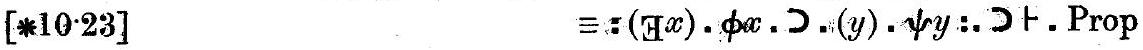
\includegraphics[max width=\textwidth, alt={}, center]{bc1848bf-39e8-4760-b069-9936044df683-032_50_1143_351_222}\\
＊1154． । ：$(\mathrm{H} x, y) \cdot \phi x \cdot \psi y \cdot \equiv:(\mathrm{H} x) \cdot \phi x:(\mathrm{H} y) \cdot \psi y$\\
Dem．\\
＋．＊1035．ɔㅇ：$(\square y) \cdot \phi x \cdot \psi y . \quad \equiv: \phi x:(\neg y) \cdot \psi y:$.\\
$[* 10 \cdot 11 \cdot 281]$ ）$:\left(\mathrm{H}^{x}, y\right) \cdot \phi x \cdot \psi y \cdot \equiv:(\mathrm{H} x): \phi x:(\mathrm{H} y) \cdot \psi y:$\\
［＊1035］三：（Gx）．$\phi x:($ J $y) \cdot \psi y:$ ．J？Prop\\
This proposition is very often used．\\
＊1155．$\quad \vdash:(\mathbb{T} x, y) \cdot \phi x \cdot \psi(x, y) \cdot \equiv:(\mathbb{T} x): \phi x:(\mathrm{H} y) \cdot \psi(x, y)$\\
Dem．\\
ト．$* 10: 35$ ． ग $:($ 月 $y) \cdot \phi x \cdot \psi(x, y) . \quad \equiv: \phi x:($ 马 $y) \cdot \psi(x, y):$.\\
［＊10．11］D $\vdash:(x):(\mathrm{H} y) \cdot \phi x \cdot \psi(x, y) \cdot \equiv: \phi x:(\mathrm{H} y) \cdot \psi(x, y):$.\\
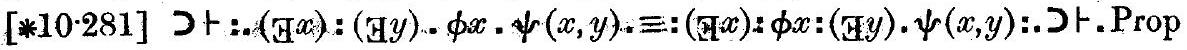
\includegraphics[max width=\textwidth, alt={}, center]{bc1848bf-39e8-4760-b069-9936044df683-032_50_1187_902_224}\\
This proposition is very often used．\\
＊11：56．$\vdash:(x) \cdot \phi x:(y) \cdot \psi y: \equiv:(x, y) \cdot \phi x \cdot \psi y$\\
Dem．


\begin{align*}
& \text { ト.*1033. ɔト:: }(x) . \phi x:(y) . \psi y: \equiv: .(x): . \phi x:(y) . \psi y  \tag{1}\\
& \text { ト. } * 1033 . \text { つ }: . \quad \phi x:(y), \psi y: \equiv:(y) . \phi x . \psi y: . \\
& \text { [*10:11] ɔト:. }(x):-\phi x:(y), \psi y: \equiv:(y) . \phi x . \psi y: . \\
& {[* 10 \cdot 271] \text { วト: }(x): . \phi x:(y) \cdot \psi y: \equiv:(x):(y) \cdot \phi x \cdot \psi y:} \\
& {[(* 11 \cdot 01)] \quad \equiv:(x, y) \cdot \phi x \cdot \psi y}  \tag{2}\\
& \text { ト.(1).(2). ɔћ.Prop }
\end{align*}


＊1157．$\vdash:(x) . \phi x . \equiv .(x, y) . \phi x . \phi y$［＊1156．＊4－24］\\
The use of＊4：24 here depends upon the fact that（x）．$\phi x$ and（y）．$\phi y$ are the same proposition．\\
＊1158．$+:\left(H^{x}\right) \cdot \phi x \equiv\left(H^{x}, y\right) \cdot \phi x \cdot \phi y \quad[* 11: 54 \cdot * 4 \cdot 24]$\\
＊1159． 人 $: \phi x . \nu_{x} . \psi x: \equiv: \phi x . \phi y . \nu_{x, y} . \psi x . \psi y$\\
Dem．


\begin{align*}
& \text { ト.*11.57.つト:. } \phi x . \partial_{x} . \psi x: \equiv:(x, y): \phi x . \text { ɔ. } \psi x: \phi y \text {. Э. } \psi y \text { : } \\
& \text { [*3.47.*11:32] つ:(x,y): } \phi x . \phi y . \supset . \psi x . \psi y  \tag{1}\\
& \text { ト.*111. ɔ :. }(x, y): \phi x . \phi y . \supset . \psi x . \psi y: \supset: \phi x . \phi y . \supset . \psi x . \psi y  \tag{2}\\
& \text { ト.(2) } \frac{x}{y} \cdot * 4 \cdot 24 . \text { つ }:: \mathrm{Hp}(2) \cdot \text { ɔ : } \phi x \cdot \text { ɔ } \psi x  \tag{3}\\
& \text { ト.(3).*10.11.21.ɔ } \\
& \text { ⊢ :. }(x, y): \phi x . \phi y . \supset . \psi x . \psi y: \supset: \phi x . \supset_{x} . \psi x  \tag{4}\\
& \text { ト.(1).(4). ɔ . Prop }
\end{align*}


＊11．6．$F::(\mathrm{H} x): .(\mathrm{H} y) . \phi(x, y) . \psi y: \chi^{x}: . \equiv: .(\mathrm{H} y): .(\mathrm{H} x) . \phi(x, y) . \chi^{x}: \psi y$\\
This proposition is very frequently employed in subsequent proofs．\\
Dem．\\
ト．＊10．35．ɔト：．（马y）．$\phi(x, y) \cdot \psi y: \chi^{x}: \equiv:(\mathrm{H} y): \phi(x, y) \cdot \psi y \cdot \chi^{x}:$.\\
$[* 10 \cdot 11 \cdot 281]$ ว $+:\left(\mathrm{H}^{x}\right):(\mathrm{H} y) \cdot \phi(x, y) \cdot \psi y: \chi x:$\\
［＊11－23］

$$
\equiv:\left(H^{x}\right):(H y) \cdot \phi(x, y) \cdot \psi y \cdot \chi x: .
$$

［＊11：341．Perm］\\
$\equiv: .(\mathrm{G} y): .(\mathrm{G} x) . \phi(x, y) . \psi y \cdot \chi x:$.\\
［＊10．35．281］\\
$\equiv: .(\mathrm{H} y): .(\mathrm{H} x) \cdot \phi(x, y) \cdot \chi^{x} \cdot \psi y:$.\\
$\equiv: .($ Ty $y): .($ T $x) . \phi(x, y) . \chi^{x}: \psi y:: \supset \vdash$. Prop\\
＊1161．$\vdash:(\mathrm{H} y): \phi x . \partial_{x} . \psi(x, y): \supset: \phi x . \partial_{x} \cdot(\mathrm{H} y) \cdot \psi(x, y)$\\
Dem．\\
ト．＊11．26．ɔ ：：Hp．ɔ ：．（ $x$ ）：．（ $\mathrm{H} y$ ）：$\phi x$. つ ．$\psi(x, y)$

ト ．$* 1037$ ．ɔ $: .(\mathrm{H} y): \phi x . \supset . \psi(x, y): \supset: \phi x . \supset .(\mathrm{H} y) . \psi(x, y):$.\\
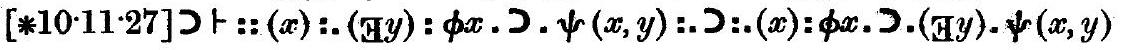
\includegraphics[max width=\textwidth, alt={}, center]{bc1848bf-39e8-4760-b069-9936044df683-033_50_1121_798_137}

ト．（1）．（2）．ɔ ．Prop\\
＊1162．$\vdash:: \phi x \cdot \psi(x, y) \cdot \partial_{x, y} \cdot \chi(x, y): \equiv: \phi x \cdot \partial_{x}: \psi(x, y) \cdot \partial_{y} \cdot \chi(x, y)$\\
Dem．\\
ト．＊4：87．＊111133．ɔ\\
$\vdash:: \phi x \cdot \psi(x, y) \cdot \nu_{x, y} \cdot \chi(x, y): \equiv: .(x, y):, \phi x . \supset: \psi(x, y) . \supset \cdot \chi(x, y)$\\
［＊10．21．11．271］

$$
\begin{array}{r}
\equiv:(x): \phi x . \supset:(y): \psi(x, y) \cdot \supset \cdot \chi(x, y):= \\
\text { つㄱ.Prop }
\end{array}
$$

＊1163．$\vdash: . \sim(G x, y) . \phi(x, y) . \supset: \phi(x, y) . \partial_{x, y} . \psi(x, y)$\\
Dem．\\
$\vdash . * 2 * 21 . * 11$ 11．ɔ ：．$(x, y): \sim \phi(x, y) . \supset: \phi(x, y) .3 . \psi(x, y):$.\\
［＊1132］$\quad \supset+:(x, y) \sim \phi(x, y) . \supset:(x, y): \phi(x, y) . \supset . \psi(x, y):$.\\
［＊11．25］\\
$\supset \vdash: \sim(\mathbb{H} x, y) \cdot \phi(x, y) \cdot \supset:(x, y): \phi(x, y) \cdot \supset \cdot \psi(x, y):$. ɔㄴ．Prop\\
＊117．

$$
\vdash:(\mathrm{H} x, y): \phi(x, y) \cdot v \cdot \phi(y, x): \equiv \cdot(\mathrm{H} x, y) \cdot \phi(x, y)
$$

Dem．\\
$\vdash \cdot * 1141$. つ $\vdash:(\mathcal{H} x, y): \phi(x, y) \cdot v \cdot \phi(y, x):$\\
［＊11：23］

$$
\begin{aligned}
& \equiv:(\mathbb{H} x, y) \cdot \phi(x, y) \cdot v \cdot(G x, y) \cdot \phi(y, x): \\
& \equiv:(H x, y) \cdot \phi(x, y) \cdot v \cdot(H y, x) \cdot \phi(y, x): \\
& \equiv:(H x, y) \cdot \phi(x, y): \supset f \cdot \text { Prop }
\end{aligned}
$$

［＊4：25］\\
In the last line of the above proof，use is made of the fact that

$$
\left(H^{x}, y\right) \cdot \phi(x, y) \text { and }(H y, x) \cdot \phi(y, x)
$$

are the same proposition．\\
The first use of the following proposition occurs in the proof of $* 234 \cdot 12$ ． Its utility lies in its enabling us to pass from a hypothesis

$$
\phi z \cdot \chi w \cdot J_{z, w} \cdot \psi z \cdot \theta w,
$$

containing two apparent variables，to the product of two hypotheses each containing only one．\\
＊1171．$\vdash::\left(\mathrm{H}^{z}\right) \cdot \phi z:\left(\mathrm{H}^{w}\right) \cdot \chi w: \supset:$.\\
Dem．

$$
\phi z \cdot \partial_{z} \cdot \psi z: \chi w \cdot \partial_{w} \cdot \theta w: \equiv: \phi z \cdot \chi w \cdot \partial_{z, w} \cdot \psi z \cdot \theta w
$$

$\vdash . * 10 \cdot 1 . * 3.47$. つ $: . \phi z$. つ $_{z} . \psi z: \chi w$. J $_{w} . \theta w:$


\begin{equation*}
\nu: \phi z \cdot \chi w \cdot \nu \cdot \psi z \cdot \theta w \tag{1}
\end{equation*}


$\vdash .(1) . * 11 \cdot 113 . \supset \vdash: . \phi z . \omega_{z} . \psi z: \chi w . \omega_{w} . \theta w:$


\begin{equation*}
\nu: \phi z \cdot \chi w \cdot J_{z, w} \cdot \psi z \cdot \theta w \tag{2}
\end{equation*}


$\vdash \cdot * 10 \cdot 1 . \supset \vdash:: \phi z \cdot \chi w . \partial_{z, w} \cdot \psi z \cdot \theta w: \supset: \phi z \cdot \chi w \cdot \partial_{w} \cdot \psi z \cdot \theta w:$.\\
［＊10．28］ɔ：．（马w）．$\phi z \cdot \chi w \cdot \nu \cdot(\mathrm{H} w) \cdot \psi z \cdot \theta w:$\\
［＊10：35］ɔ：．$\phi z:($ 月 $w) \cdot \chi w: \supset: \psi z:($ 万 $w) \cdot \theta w$


\begin{equation*}
\vdash .(3) . C o m m . * 326 . \supset \vdash::(G w) . \chi w: \supset: . \phi z \cdot \chi w . \partial_{z, w} . \psi z . \theta w: \tag{3}
\end{equation*}



\begin{equation*}
\supset: \phi z \cdot \supset \cdot \psi z \tag{4}
\end{equation*}


$\vdash .(4) . * 10 \cdot 11 \cdot 21 . \supset \vdash::(H w) \cdot \chi w . \supset: . \phi z \cdot \chi^{w} \cdot \partial_{z, w} \cdot \psi z \cdot \theta w:$


\begin{equation*}
\nu: \phi z \cdot \nu_{z} \cdot \psi z \tag{5}
\end{equation*}


Similarly

\[
\begin{array}{r}
\vdash::\left(\mathrm{G}^{z}\right) \cdot \phi z \cdot \supset: \phi z \cdot \chi^{w} \cdot \partial_{z, w} \cdot \psi z \cdot \theta w: \\
\supset: \chi^{w} \cdot \partial_{w} \cdot \theta w \tag{6}
\end{array}
\]

ト．（5）．（6）．＊3．47．Comp．ɔ


\begin{equation*}
\vdash:: \mathrm{Hp} . \supset: \phi z \cdot \chi^{w} . \partial_{z, w} . \psi z . \theta w: \supset: \phi z . \partial_{z} . \psi z: \chi^{w} . \partial_{w} . \theta w \tag{7}
\end{equation*}


ト．（2）．（7）．ɔㄴ．Prop

\section*{*12. THE HIERARCHY OF TYPES AND THE AXIOM OF REDUCIBILITY}
The primitive idea " $(x) \cdot \phi x$ " has been explained to mean " $\phi x$ is always true," i.e. "all values of $\phi x$ are true." But whatever function $\phi$ may be, there will be arguments $x$ with which $\phi x$ is meaningless, i.e. with which as arguments $\phi$ does not have any value. The arguments with which $\phi x$ has values form what we will call the "range of significance" of $\phi x$. A "type" is defined as the range of significance of some function. In virtue of $* 9 \cdot 14$, if $\phi x, \phi y$, and $\psi x$ are significant, i.e. either true or false, so is $\psi y$. From this it follows that two types which have a common member coincide, and that two different types are mutually exclusive. Any proposition of the form (x). $\phi x$, i.e. any proposition containing an apparent variable, determines some type as the range of the apparent variable, the type being fixed by the function $\phi$.

The division of objects inta types is necessitated by the vicious-circle fallacies which otherwise arise*. These fallacies show that there must be no totalities which, if legitimate, would contain members defined in terms of themselves. Hence any expression containing an apparent variable must not be in the range of that variable, i.e. must belong to a different type. Thus the apparent variables contained or presupposed in an expression are what determines its type. This is the guiding principle in what follows.

As explained in $* 9$, propositions containing variables are generated from propositional functions which do not contain these apparent variables, by the process of asserting all or some values of such functions. Suppose $\phi a$ is a proposition containing $a$; we will give the name of generalization to the process which turns $\phi a$ into $(x) \cdot \phi x$ or $(G x) \cdot \phi x$, and we will give the name of generalized propositions to all such as contain apparent variables. It is plain that propositions containing apparent variables presuppose others not containing apparent variables, from which they can be derived by generalization. Propositions which contain no apparent variables we call elementary propositions † , and the terms of such propositions, other than functions, we call individuals. Then individuals form the first type.

It is unnecessary, in practice, to know what objects belong to the lowest type, or even whether the lowest type of variable occurring in a given context is that of individuals or some other. For in practice only the relative types of variables are relevant; thus the lowest type occurring in a given context may be called that of individuals, so far as that context is concerned. Accordingly the above account of individuals is not essential to the truth of what

\footnotetext{\begin{itemize}
  \item Cf. Introduction, Chapter II.\\
† Cf. pp. 91, 92.
\end{itemize}
}
follows; all that is essential is the way in which other types are generated from individuals, however the type of individuals may be constituted.

By applying the process of generalization to individuals occurring in elementary propositions, we obtain new propositions. The legitimacy of this process requires only that no individuals should be propositions. That this is so, is to be secured by the meaning we give to the word individual. We may explain an individual as something which exists on its own account; it is then obviously not a proposition, since propositions, as explained in Chapter II of the Introduction (p. 43), are incomplete symbols, having no meaning except in use. Hence in applying the process of generalization to individuals we run no risk of incurring reflexive fallacies. We will give the name of first-order propositions to such as contain one or more apparent variables whose possible values are individuals, but contain no other apparent variables. First-order propositions are not all of the same type, since, as was explained in $* 9$, two propositions which do not contain the same number of apparent variables cannot be of the same type. But owing to the systematic ambiguity of negation and disjunction, their differences of type may usually be ignored in practice. No reflexive fallacies will result, since no first-order proposition involves any totality except that of individuals.

Let us denote by " $\phi!\hat{x}$ " or " $\phi!(\hat{x}, \hat{y})$ " or etc. an elementary function whose argument or arguments are individual. We will call such a function a predicative function of an individual. Such functions, together with those derived from them by generalization, will be called first-order functions. In practice we may without risk of reflexive fallacies treat first-order functions as a type, since the only totality they involve is that of individuals, and, by means of the systematic ambiguity of negation and disjunction, any function of a first-order function which will concern us will be significant whatever first-order function is taken as argument, provided the right meanings are given to the negations and disjunctions involved.

For the sake of clearness, we will repeat in somewhat different terms our account of what is meant by a first-order function. Let us give the name of matrix to any function, of however many variables, which does not involve any apparent variables. Then any possible function other than a matrix is derived from a matrix by means of generalization, i.e. by considering the proposition which asserts that the function in question is true with all possible values or with some value of one of the arguments, the other argument or arguments remaining undetermined. Thus e.g. from the function $\phi(x, y)$ we shall be able to derive the four functions

$$
(x) \cdot \phi(x, y), \quad\left(\mathrm{H}^{x}\right) \cdot \phi(x, y), \quad(y) \cdot \phi(x, y), \quad(\text { Hy }) \cdot \phi(x, y),
$$

of which the two first are functions of $y$, while the two last are functions of $x$. (All propositions, with the exception of such as are values of matrices, are also derived from matrices by the above process of generalization. In order to obtain\\
a proposition from a matrix containing $n$ variables, without assigning values to any of the variables, it is necessary to turn all the variables into apparent variables. Thus if $\phi(x, y)$ is a matrix, $(x, y) \cdot \phi(x, y)$ is a proposition.) We will give the name first-order matrices to such as have only individuals for their arguments, and we will give the name of first-order functions (of any number of variables) to such as either are first-order matrices or are derived from first-order matrices by generalization applied to some (not all) of the arguments to such matrices. First-order propositions will be such as result from applying generalization to all the arguments to a first-order matrix.

As we have already stated, the notation " $\phi!\hat{z}$ " is used for any elementary function of one variable. Thus " $\phi!x$ " represents any value of any elementary function of one variable. It will be seen that " $\phi!x$ " is a function of two variables, namely $\phi!\hat{z}$ and $x$. Since it contains no apparent variable, it is a matrix, but since it contains a variable (namely $\phi!\hat{z}$ ) which is not an individual, it is not a first-order matrix. The same applies to $\phi!\alpha$, where $a$ is some definite constant. We can build up a number of new matrices, such as

$$
\begin{aligned}
& \sim \phi!a, \quad \sim \phi!x, \quad \phi!x \vee \phi!y, \quad \phi!x \vee \psi!x, \quad \phi!x \vee \psi!y, \\
& \phi!x . \supset \cdot \psi!x, \quad \phi!x . \psi!x, \quad \phi!x \vee \psi!y \vee \chi!z, \text { and so on. }
\end{aligned}
$$

All these are matrices which involve first-order functions among their arguments. Such matrices we will call second-order matrices. From these matrices, by applying generalization to their arguments, whether to such as are functions or to such (if any) as are individuals, we obtain new functions and propositions. Such functions (together with second-order matrices) will be called secondorder functions, and such propositions will be called second-order propositions. Thus we are led to the following definitions:

A second-order matrix is one which has at least one first-order matrix among its arguments, but has no arguments other than first-order matrices and individuals.

A second-order function is one which either is a second-order matrix or results from one by applying generalization to some (not all) of the arguments to a second-order matrix.

A second-order proposition is one which results from a second-order matrix by applying generalization to all its arguments.

In addition to the above illustrations of second-order matrices, we may give the following examples of second-order functions:\\
(1) Functions in which the argument is $\phi!\hat{z}:(x) \cdot \phi!x$, (Tx) $\cdot \phi!x$, $\phi!a . \supset . \phi!b$, where $a$ and $b$ are constants, $\phi!x . \partial_{x} . g!x$, where $g!\hat{z}$ is a constant function, and so on.\\
(2) Functions in which the arguments are $\phi!\hat{z}$ and $\psi!\hat{z}$ :

$$
\phi!x \cdot \partial_{x} \cdot \psi!x, \quad \phi!x \cdot \equiv_{x} \cdot \psi!x, \quad\left(\mathbb{H}^{x}\right) \cdot \phi x \cdot \psi x, \quad \phi!a \cdot \supset \cdot \psi!b,
$$

where $a$ and $b$ are constants, and so on\\
(3) Functions in which the argument is an individual $x:(\phi) \cdot \phi!x$, $($ I $\phi) . \phi!x, \phi!x . \partial_{\phi} . \phi!a$, where $a$ is constant, and so on.\\
(4) Functions in which the arguments are $\phi!\hat{z}$ and $x: \phi!x, \phi!x . \supset . \phi!a$, where $a$ is constant, ( $H \psi$ ) : $\phi!x . \equiv . \psi!x$, and so on.

Examples of second-order functions might, of course, be multiplied indefinitely, but the above seem sufficient for purposes of illustration.

A second-order matrix of one variable will be called a predicative secondorder function of one variable or a predicative function of a first-order matrix. Thus $\phi!a, \sim \phi!a$ and $\phi!a \supset \phi!b$ are predicative functions of $\phi!\hat{z}$. Similarly a function of several variables of which at least one is a first-order matrix, while the rest are either individuals or first-order matrices, will be called predicative if it is a matrix.

It will be seen, however, that a second-order function may have only individuals for its arguments; instances were given just now under the heading (3). Such functions we shall not call predicative, since predicative functions of individuals have already been defined as being such as are of the first order. Thus the order of a function is not determined by the order of its argument or arguments; indeed, the function may be of any order superior to the order or orders of its arguments.

A variable matrix whose argument is $\phi!\hat{z}$ will be denoted by $f!\phi!\hat{z}$, and generally, a matrix whose arguments are $\phi!\hat{z}, \psi!\hat{z}, \ldots x, y, \ldots$ (where there is at least one function among the arguments) will be denoted by

$$
f!(\phi!\hat{z}, \psi!\hat{z}, \ldots x, y, \ldots)
$$

Such a matrix is not of the first or second order, since it contains the new variable $f$, whose values are second-order matrices. We proceed to construct new matrices as we did with the matrix $\phi!\hat{x}$; these constitute third-order matrices. These together with the functions derived from them by generalization are called third-order functions, and the propositions derived from thirdorder matrices by generalization are called third-order propositions.

In this way we can proceed indefinitely to matrices, functions and propositions of higher and higher orders. We introduce the following definition:

A function is said to be predicative when it is a matrix. It will be observed that, in a hierarchy in which all the variables are individuals or matrices, a matrix is the same thing as an elementary function (cf. pp. 127, 128).\\
"Matrix" or "predicative function" is a primitive idea.\\
The fact that a function is predicative is indicated, as above, by a note of exclamation after the functional letter.

The variables occurring in the present work, from this point onwards, will all be either individuals or matrices of some order in the above hierarchy. Propositions, which have occurred hitherto as variables, will no longer do so\\
except in a few isolated cases of which no subsequent use is made. In practice, for the reasons explained on p. 162, a function of a matrix may be regarded as capable of any argument which is a function of the same order and takes arguments of the same type.

In practice, we never need to know the absolute types of our variables, but only their relative types. That is to say, if we prove any proposition on the assumption that one of our variables is an individual, and another is a function of order $n$, the proof will still hold if, in place of an individual, we take a function of order $m$, and in place of our function of order $n$ we take a function of order $n+m$, with corresponding changes for any other variables that may be involved. This results from the assumption that our primitive propositions are to apply to variables of any order.

We shall use small Latin letters (other than $p, q, r, s$ ) for variables of the lowest type concerned in any context. For functions, we shall use the letters $\phi, \psi, \chi, \theta, f, g, F$ (except that, at a later stage, $F$ will be defined as a constant relation, and $\theta$ will be defined as the order-type of the continuum).

We shall explain later a different hierarchy, that of classes and relations, which is derived from the functional hierarchy explained above, but is more convenient in practice.

When any predicative function, say $\phi!\hat{z}$, occurs as apparent variable, it would be strictly more correct to indicate the fact by placing " $(\phi!\hat{z})$ " before what follows, as thus: " $(\phi!\hat{z}) \cdot f(\phi!\hat{z})$." But for the sake of brevity we write simply " $(\phi)$ " instead of " $(\phi!\hat{z})$." Since what follows the $\phi$ in brackets must always contain $\phi$ with arguments supplied, no confusion can result from this practice.

It should be observed that, in virtue of the manner in which our hierarchy of functions was generated, non-predicative functions always result from such as are predicative by means of generalization. Hence it is unnecessary to introduce a special notation for non-predicative functions of a given order and taking arguments of a given order. For example, second-order functions of an individual $x$ are always derived by generalization from a matrix

$$
f!(\phi!\hat{z}, \psi!\hat{z}, \ldots x, y, z, \ldots),
$$

where the functions $f, \phi, \psi, \ldots$ are predicative. It is possible, therefore, without loss of generality, to use no apparent variables except such as are predicative.

We require, however, a means of symbolizing a function whose order is not assigned. We shall use " $\phi x$ " or " $f(\chi!\hat{z})$ " or etc. to express a function ( $\phi$ or $f$ ) whose order, relatively to its argument, is not given. Such a function cannot be made into an apparent variable, unless we suppose its order previously fixed. As the only purpose of the notation is to avoid the necessity of fixing the order, such a function will not be used as an apparent variable; the only functions which will be so used will be predicative functions, because, as we have just seen, this restriction involves no loss of generality.

We have now to state and explain the axiom of reducibility.\\
It is important to observe that, since there are various types of propositions and functions, and since generalization can only be applied within some one type (or, by means of systematic ambiguity, within some well-defined and completed set of types), all phrases referring to "all propositions" or "all functions," or to "some (undetermined) proposition" or "some (undetermined) function," are prima facie meaningless, though in certain cases they are capable of an unobjectionable interpretation. Contradictions arise from the use of such phrases in cases where no innocent meaning can be found.

If mathematics is to be possible, it is absolutely necessary (as explained in the Introduction, Chapter II) that we should have some method of making statements which will usually be equivalent to what we have in mind when we (inaccurately) speak of "all properties of $x$." (A "property of $x$ " may be defined as a propositional function satisfied by $x$.) Hence we must find, if possible, some method of reducing the order of a propositional function without affecting the truth or falsehood of its values. This seems to be what commonsense effects by the admission of classes. Given any propositional function $\psi x$, of whatever order, this is assumed to be equivalent, for all values of $x$, to a statement of the form " $x$ belongs to the class $\alpha$." Now assuming that there is such an entity as the class $\alpha$, this statement is of the first order, since it involves no allusion to a variable function. Indeed its only practical advantage over the original statement $\psi x$ is that it is of the first order. There is no advantage in assuming that there really are such things as classes, and the contradiction about the classes which are not members of themselves shows that, if there are classes, they must be something radically different from individuals. It would seem that the sole purpose which classes serve, and one main reason which makes them linguistically convenient, is that they provide a method of reducing the order of a propositional function. We shall, therefore, not assume anything of what may seem to be involved in the common-sense admission of classes, except this, that every propositional function is equivalent, for all its values, to some predicative function of the same argument or arguments.

This assumption with regard to functions is to be made whatever may be the type of their arguments. Let $f u$ be a function, of any order, of an argument $u$, which may itself be either an individual or a function of any order. If $f$ is a matrix, we write the function in the form $f!u$; in such a case we call $f$ a predicative function. Thus a predicative function of an individual is a firstorder function; and for higher types of arguments, predicative functions take the place that first-order functions take in respect of individuals. We assume, then, that every function of one variable is equivalent, for all its values, to some predicative function of the same argument. This assumption seems to be the essence of the usual assumption of classes; at any rate, it retains as much\\
of classes as we have any use for, and little enough to avoid the contradictions which a less grudging admission of classes is apt to entail. We will call this assumption the axiom of classes, or the axiom of reducibility.

We shall assume similarly that every function of two variables is equivalent, for all its values, to a predicative function of those variables, i.e. to a matrix. This assumption is what seems to be meant by saying that any statement about two variables defines a relation between them. We will call this assumption the axiom of relations or (like the previous axiom) the axiom of reducibility.

In dealing with relations between more than two terms, similar assumptions would be needed for three, four, ... variables. But these assumptions are not indispensable for our purpose, and are therefore not made in this work.

Stated in symbols, the two forms of the axiom of reducibility are as follows:

\[
\begin{array}{ll}
\vdash:(\mathrm{H} f): \phi x \cdot \equiv_{x} \cdot f!x & \mathrm{Pp} \\
\vdash:(\mathrm{H} f): \phi(x, y) \cdot \equiv_{x, y} \cdot f!(x, y) & \mathrm{Pp} \tag{$* 12 \cdot 11$}
\end{array}
\]

We call two functions $\phi \hat{x}, \psi \hat{x}$ formally equivalent when $\phi x \cdot \Xi_{x} \cdot \psi x$, and similarly we call $\phi(\hat{x}, \hat{y})$ and $\psi(\hat{x}, \hat{y})$ formally equivalent when

$$
\phi(x, y) \cdot \equiv_{x, y \cdot \psi}(x, y) .
$$

Thus the above axioms state that any function of one or two variables is formally equivalent to some predicative function of one or two variables, as the case may be.

Of the above two axioms, the first is chiefly needed in the theory of classes $(* 20)$, and the second in the theory of relations (*21). But the first is also essential to the theory of identity, if identity is to be defined (as we have done, in $* 13.01$ ); its use in the theory of identity is embodied in the proof of $* 13.101$, below.\\
-We may sum up what has been said in the present number as follows:\\
(1) A function of the first order is one which involves no variables except individuals, whether as apparent variables or as arguments.\\
(2) A function of the $(n+1)$ th order is one which has at least one argument or apparent variable of order $n$, and contains no argument or apparent variable which is not either an individual or a first-order function or a second-order function or ... or a function of order $n$.\\
(3) A predicative function is one which contains no apparent variables, i.e. is a matrix. It is possible, without loss of generality, to use no variables except matrices and individuals, so long as variable propositions are not required.\\
(4) Any function of one argument or of two is formally equivalent to a predicative function of the same argument or arguments.

\section*{*13. IDENTITY}
Summary of *13.\\
The propositional function " $x$ is identical with $y$ " will be written " $x=y$." We shall find that this use of the sign of equality covers all the common uses of equality that occur in mathematics. The definition is as follows:\\
*13.01. $x=y .=:(\phi): \phi!x$. J. $\phi!y$ Df\\
This definition states that $x$ and $y$ are to be called identical when every predicative function satisfied by $x$ is also satisfied by $y$. We cannot state that every function satisfied by $x$ is to be satisfied by $y$, because $x$ satisfies functions of various orders, and these cannot all be covered by one apparent variable. But in virtue of the axiom of reducibility it follows that, if $x=y$ and $x$ satisfies $\psi x$, where $\psi$ is any function, predicative or non-predicative, then $y$ also satisfies $\psi y$ (cf. $* 13 \cdot 101$, below). Hence in effect the definition is as powerful as it would be if it could be extended to cover all functions of $x$.

Note that the second sign of equality in the above definition is combined with "Df," and thus is not really the same symbol as the sign of equality which is defined. Thus the definition is not circular, although at first sight it appears so.

The propositions of the present number are constantly referred to. Most of them are self-evident, and the proofs offer no difficulty. The most important of the propositions of this number are the following:\\
*13.101. $\vdash: x=y$. つ . $\psi x$ つ $\psi y$\\
I.e. if $x$ and $y$ are identical, any property of $x$ is a property of $y$.\\
*13.12. $\mathrm{F}: x=y$. J.$\psi x \equiv \psi y$\\
This includes *13-101 together with the fact that if $x$ and $y$ are identical any property of $y$ is a property of $x$.\\
*13.15.16.17, which state that identity is reflexive, symmetrical and transitive.\\
*13.191. $\vdash:, y=x . \supset_{y} . \phi y: \equiv . \phi x$\\
I.e. to state that everything that is identical with $x$ has a certain property is equivalent to stating that $x$ has that property.\\
*13.195. $\vdash:($ H $y) \cdot y=x \cdot \phi y \cdot \equiv \cdot \phi x$\\
I.e. to state that something identical with $x$ has a certain property is equivalent to saying that $x$ has that property.\\
*1322. $\mathrm{F}:(\mathrm{H} z, w) \cdot z=x \cdot w=y \cdot \phi(z, w) \cdot \equiv \cdot \phi(x, y)$\\
This is the analogue of $* 13 \cdot 195$ for two variables.\\
＊13．01．$x=y .=:(\phi): \phi!x$. ɔ．$\phi!y$ Df\\
The following definitions embody abbreviations which are often convenient．\\
＊13．02．$x \neq y .=. \sim(x=y) \quad$ Df\\
＊13．03．$x=y=z .=. x=y . y=z$ Df\\
＊131．F：$x=y . \equiv: \phi!x . \partial_{\phi} . \phi!y[* 4 \cdot 2 .(* 13 \cdot 01) .(* 10 \cdot 02)]$\\
＊13101．$\vdash: x=y$. ɔ.$\psi x$ つ $\psi y$\\
Dem．\\
ト．＊121． つ ：：$($ H $\phi): . \psi x . \equiv . \phi!x: \psi y . \equiv . \phi!y$

ト．＊131．ɔ ：：Hp．ɔ：$\phi!x . \partial_{\phi} . \phi!y$ ：．\\
$[* 4 \cdot 84 \cdot 85 . * 10 \cdot 27] \quad \supset: \psi x . \equiv \phi!x: \psi y . \equiv \phi!y: \partial_{\phi}: \psi x . \supset . \psi y:$.\\
［＊10．23］$\supset:(\mathrm{H} \phi): \psi x . \equiv . \phi!x: \psi y . \equiv . \phi!y: \supset: \psi x . \supset . \psi y$（2）\\
ト．（1）．（2）．ɔ + ．Prop\\
In virtue of this proposition，if $x=y, y$ satisfies any function，whether predicative or non－predicative，which is satisfied by $x$ ．It will be observed that the proof uses the axiom of reducibility（＊12．1）．But for this axiom，two terms $x$ and $y$ might agree in respect of all predicative functions，but not in respect of all non－predicative functions．We should thus be led to identities of different degrees，according to the degree of the functions in respect of which $x$ and $y$ agreed．Strict identity would，in this case，have to be taken as a primitive idea，and $* 13 \cdot 101$ would have to be a primitive proposition，as would also $* 13 \cdot 15 \cdot 16 \cdot 17$ ．\\
＊13：11． ト：$: x=y . \equiv: \phi!x . \equiv_{\phi} . \phi!y$\\
Dem．


\begin{align*}
& \text { ト.*10.22. ɔト:. } \phi!x . \equiv_{\phi} . \phi!y: \supset: \phi!x . J_{\phi} . \phi!y \text { : } \\
& \text { [*13•1] ɔ:x=y }  \tag{1}\\
& \text { ト. } * 13101 \text {. ɔ :. } x=y . \text { ɔ. } \phi!x \text { ɔ } \phi!y  \tag{2}\\
& \text { ト. } * 13 \cdot 101 . * 1 \text { ⋅ } . \supset \vdash: x=y . \supset . \sim \phi!x \supset \sim \phi!y \text {. } \\
& \text { [Transp] ɔ.φ!y ɔφ!x }  \tag{3}\\
& \text { ト.(2).(3).Comp.ɔ : } x=y \text {. ɔ. } \phi!x \equiv \phi!y \text { : } \\
& \text { [*10.11.21] ɔト:. } x=y . \supset: \phi!x . \equiv_{\phi} . \phi!y  \tag{4}\\
& \text { ト.(1).(4). ɔト.Prop }
\end{align*}


＊13．12．$\vdash: x=y$. J.$\psi x \equiv \psi y$\\
Dem．

$$
\begin{aligned}
& \vdash \cdot * 13 \cdot 101 \text {. Comp. } \partial \vdash: x=y \cdot \supset \cdot \psi x \supset \psi y \cdot \sim \psi x \supset \sim \psi y . \\
& {[\text { Transp] } \quad \text { つ. } \psi x \equiv \psi y: \supset \vdash . \text { Prop }}
\end{aligned}
$$

＊13．13．$\vdash: \psi x . x=y: \supset . \psi y$\\
＊1314．$\vdash: \psi x . \sim \psi y . \supset . x \neq y$\\
＊1315．ト．$x=x$\\
＊13•16．$\vdash: x=y . \equiv . y=x$\\
［＊13．101．Comm．Imp］\\
［＊13•13．＊4•14］\\
［Id．＊10．11．＊13．1］\\
［＊13．11．＊10．32］\\
＊13．17．$\vdash: x=y . y=z$. つ．$x=z$\\
Dem．

$$
\begin{aligned}
& \vdash . * 13.1 . \supset \vdash:: \text { Hp } . \supset: \phi!x . \partial_{\phi} . \phi!y: \phi!y . \partial_{\phi} . \phi!z: . \\
& {[* 10: 3] \quad \supset: \phi!x . \partial_{\phi} . \phi!z:: \supset \vdash . \text { Prop }}
\end{aligned}
$$

In the above use of $* 10 \cdot 3, \phi!x, \phi!y, \phi!z$ are regarded as three different functions of $\phi$ ，and $\phi$ replaces the $x$ of $* 10 \cdot 3$ ．

The above three propositions show that identity is reflexive（＊13．15）， symmetrical（＊13．16），and transitive（＊13．17）．These are the three marks of relations having the formal properties which we associate commonly with the sign of equality．\\
＊13．171．$\leqslant: x=y . x=z$. J．$y=z \quad[* 13.16 .17]$\\
＊13．172． $\mathrm{F}: y=x . z=x$. J．$y=z \quad[* 13.16 \cdot 17]$\\
＊13．18． $\mathrm{F}: x=y . x \neq z$. J．$y \neq z \quad$［＊13．17．＊4．14］\\
＊13．181． $\mathrm{F}: x=y . y \neq z$. J．$x \neq z \quad$［＊13．171．＊4．14］\\
＊13．182．$F: . x=y$. ɔ $: z=x . \equiv . z=y$［＊13．17172．Exp．Comp］\\
＊13＇183． V ：$x=y . \equiv: z=x . \equiv_{z} . z=y$\\
Dem．


\begin{align*}
& \vdash \cdot * 13 \cdot 182 \cdot * 10 \cdot 11 \cdot 21 \cdot \supset \vdash: x=y \cdot \supset: z=x \cdot \equiv_{z} \cdot z=y  \tag{1}\\
& \vdash \cdot * 10 \cdot 1 . \quad \supset \vdash: z=x \cdot \equiv_{z} \cdot z=y: \supset: x=x \cdot \supset \cdot x=y: \\
& {[* 13 \cdot 15]}  \tag{2}\\
& \text { け.(1).(2).J+.Prop } \quad \text { つ: } x=y
\end{align*}


＊1319．ト．（H $y) \cdot y=x$［＊13•15．＊1024］\\
＊13．191． ＋：$y=x . \nu_{y} . \phi y: \equiv . \phi x$\\
Dem．


\begin{align*}
& \vdash \cdot * 10 \cdot 1 \cdot \supset \vdash: \cdot y=x \cdot \supset_{y} \cdot \phi y: \supset: x=x: \supset: \phi x: \\
& {[* 13 \cdot 15]}  \tag{1}\\
& \quad \text { つ }: \phi x \\
& \vdash \cdot * 13 \cdot 12 \cdot \supset \vdash:, y=x \cdot \supset: \phi x \cdot \supset \cdot \phi y: . \\
& {[\mathrm{Comm}] \quad \text { つ }:: \phi x \cdot \supset: y=x \cdot \supset \cdot \phi y: .}  \tag{2}\\
& {[* 10 \cdot 11 \cdot 21] \supset \vdash: \phi x \cdot \supset: y=x \cdot \supset_{y} \cdot \phi y} \\
& \vdash \cdot(1) \cdot(2) \cdot \supset \vdash . \text { Prop }
\end{align*}


This proposition is constantly used in subsequent proofs．\\
＊13．192． $\mathrm{F}: .(\mathrm{G} c): x=b . \equiv_{x} . x=c: \psi c: \equiv . \psi b$\\
Dem．


\begin{align*}
& \vdash . * 4 \cdot 2 . * 3 \cdot 2 . \supset \vdash:: \psi b . \supset: x=b . \equiv_{x} . x=b: \psi b: . \\
& \text { [*1024] } \quad \supset:\left(\mathrm{H}^{c}\right): x=b . \equiv_{x} . x=c: \psi c  \tag{1}\\
& \vdash . * 101 . \supset \vdash: x=b . \equiv_{x} . x=c: \psi c: \supset: b=b . \equiv b=c: \psi c: \\
& \text { [*5:501.*13.15] } \supset: b=c . \psi c: \\
& \text { [*13.13] ɔ:ψb }  \tag{2}\\
& \text { ト.(2). } * 10 \cdot 11 \cdot 23 . \text { つ } \text { : } \text { : }\left(\mathrm{G}^{c}\right): x=b . \equiv_{x} \cdot x=c: \psi c: \text { ɔ. } \psi b  \tag{3}\\
& \text { ト.(1).(3). ɔ }+ \text {. Prop }
\end{align*}


This proposition is useful in the theory of descriptions（＊14）．\\
＊13193．$\vdash: \phi x . x=y . \equiv . \phi y . x=y$\\
Dem．


\begin{align*}
& \text { ト. Simp. ɔト: } \phi x . x=y . \text { ɔ. } x=y  \tag{1}\\
& \text { ト.*13.13. ɔト: } \phi x . x=y . \text { つ. } \phi y  \tag{2}\\
& \text { ト. (1). (2). Comp. ɔ : } \phi x, x=y . \text { ɔ. } \phi y . x=y  \tag{3}\\
& \text { ト. *1316. Fact. ɔト: } \phi y \cdot x=y \cdot \text { ɔ. } \phi y \cdot y=x \text {. } \\
& {\left[(3) \frac{y, x}{x, y}\right] \quad \text { つ. } \phi x \cdot y=x \text {. }} \\
& \text { [*13.16.Fact] ɔ. } \phi x . x=y  \tag{4}\\
& \text { ト.(3).(4). ɔㄴ. Prop }
\end{align*}


This proposition is very often used．\\
＊13．194． $\mathrm{F}: \phi x . x=y . \equiv . \phi x . \phi y . x=y$［＊13．13．＊4．71］\\
This proposition is used in $* 37 \cdot 65$ and $* 101 \cdot 14$ ．\\
＊13．195． $\mathrm{F}:(\mathrm{a} y) \cdot y=x \cdot \phi y \cdot \equiv \phi x$\\
Dem．


\begin{align*}
& \text { ト. *3.2. *13.15. ɔト: } \phi x . \text { ɔ. } x=x . \phi x \text {. } \\
& \text { [*10.24] ɔ.(马y).y=x. } \phi y  \tag{1}\\
& \text { ト. *13.13. *10.11. ɔ : : }(y): y=x . \phi y . \supset . \phi x \text { : } \\
& \text { [*10.23] ɔト:. (廿y). } y=x . \phi y . \supset . \phi x  \tag{2}\\
& \text { ト.(1).(2). ɔト.Prop }
\end{align*}


The use of this proposition in subsequent proofs is very frequent．\\
＊13．196．$+: \sim \phi x . \equiv: \phi y . \partial_{y} . y \neq x$［＊13．195．Transp．＊10．51］\\
＊1321．$\vdash: . z=x . w=y . \partial_{z, w} . \phi(z, w): \equiv . \phi(x, y)$\\
Dem．\\
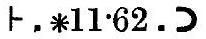
\includegraphics[max width=\textwidth, alt={}, center]{bc1848bf-39e8-4760-b069-9936044df683-045_39_206_1313_206}\\
$\vdash:: z=x . w=y . \partial_{z, w} . \phi(z, w): \equiv: . z=x . \partial_{z}: w=y . \partial_{w} . \phi(z, w):$.\\
$[* 13 \cdot 191] \quad \equiv: . w=y . \partial_{v} \cdot \phi(x, w):$.\\
［＊13•191］\\
$\equiv: . \phi(x, y):: \supset \vdash$. Prop\\
This proposition is the analogue，for two variables，of＊13．191．\\
＊1322．

$$
\vdash:\left(g^{z}, w\right) \cdot z=x \cdot w=y \cdot \phi(z, w) \cdot \equiv \cdot \phi(x, y)
$$

Dem．\\
ト．$* 11 \cdot 55$ ． ग ： ：$\left(\mathrm{H}^{z}, w\right) \cdot z=x \cdot w=y \cdot \phi(z, w)$ ．\\
［＊13•195］

$$
\begin{aligned}
& \equiv:(\mathrm{H} z): z=x:(\mathrm{H} w) \cdot w=y \cdot \phi(z, w): \\
& \equiv:(\mathrm{H} w) \cdot w=y \cdot \phi(x, w): \\
& \equiv: \phi(x, y): \text { J+.Prop }
\end{aligned}
$$

This proposition is the analogue，for two variables，of＊13195．It is fre－ quently used，especially in the theory of couples $(* 54, * 55, * 56)$ ．

The following proposition is useful in the theory of types．Its purpose is to show that，if $a$ is any argument for which＂$\phi a$＂is significant，i．e．for which we have $\phi a \mathbf{v} \sim \phi a$ ，then＂$\phi x$＂is significant when，and only when，$x$ is either\\
identical with $a$ or not identical with $a$ ．It follows（as will be proved in $* 20.81$ ） that，if＂$\phi a$＂and＂$\psi a$＂are both significant，the class of values of $x$ for which ＂$\phi x$＂is significant is the same as the class of those for which＂$\psi x$＂is signi－ ficant，i．e．two types which have a common member are identical．

In the following proof，the chief point to observe is the use of $* 10221$ ． There are two variables，$a$ and $x$ ，to be identified．In the first use，we depend upon the fact that $\phi a$ and $x=a$ both occur in both（4）and（5）：the occurrence of $\phi a$ in both justifies the identification of the two $a$＇s，and when these have been identified，the occurrence of $x=a$ in both justifies the identification of the two $x$＇s．（Unless the $a$＇s had been already identified，this would not be legitimate，because＂$x=a$＂is typically ambiguous if neither $x$ nor $a$ is of given type．）The second use of $* 10 \cdot 221$ is justified by the fact that both $\phi a$ and $\phi x$ occur in both（2）and（6）．\\
＊133．$\vdash:: \phi a \vee \sim \phi a$. J：$\phi x \vee \sim \phi x . \equiv: x=a . \vee . x \neq a$ Dem．\\
ト．$* 2 \cdot 11$ ɔ․ $\phi x \mathbf{v} \sim \phi x$

F．（1）．Simp．ɔ ：$\phi a \mathbf{v} \sim \phi a . \boldsymbol{J} . \phi x \mathbf{v} \sim \phi x$

ト．$* 2 \cdot 11$ ．$\quad \supset f: x=a \cdot \mathrm{v} \cdot x \neq a$

ト．（3）．Simp．$\supset \vdash: \phi a \mathbf{v} \sim \phi a . \supset: x=a . \mathbf{v} . x \neq a$

F ．＊13．101．Comm．ɔ ：：$\phi a \mathbf{v} \sim \phi a . \boldsymbol{\partial}: x=a . \boldsymbol{\partial} . \phi x \mathbf{v} \sim \phi x$

ト．（4）．（5）．＊10．13．221．ɔ\\
F ：：$\phi a \mathbf{v} \sim \phi a . \boldsymbol{\partial}: x=a . \mathbf{v} . x \neq a: \phi a \mathbf{v} \sim \phi a . \boldsymbol{\partial}: x=a . \boldsymbol{\partial} . \phi x \mathbf{v} \sim \phi x$

ト．（2）．（6）．＊10．13221．ɔ\\
F ：：$\phi a \mathbf{v} \sim \phi a$. J $. \phi x \mathbf{v} \sim \phi x: \phi a \mathbf{v} \sim \phi a$. J：$x=a . \mathbf{v} . x \neq a:$.\\
$\phi a \mathbf{v} \sim \phi a$. ɔ $: x=a$. J.$\phi x \mathbf{v} \sim \phi x$

ト．（7）．Simp．ɔ\\
F：：$\phi a \mathbf{v} \sim \phi a$ ． ɔ,$\phi x \mathbf{v} \sim \phi x$ ：$\phi a \mathbf{v} \sim \phi a$ ． ：$x=a$ ． $\mathbf{v}$ ．$x \neq a$

ト．（8）．＊535．$\quad \supset \vdash:: \phi a \mathbf{v} \sim \phi a . \supset: \phi x \mathbf{v} \sim \phi x . \equiv: x=a . \mathbf{v} . x \neq a::$\\
ɔㄴ．Prop

\section*{*14. DESCRIPTIONS}
\section*{Summary of *14.}
A description is a phrase of the form "the term which etc.," or, more explicitly, "the term $x$ which satisfies $\phi \hat{x}$," where $\phi \hat{x}$ is some function satisfied by one and only one argument. For reasons explained in the Introduction (Chapter III), we do not define "the $x$ which satisfies $\phi \hat{x}$," but we define any proposition in which this phrase occurs. Thus when we say : "The term $x$ which satisfies $\phi \hat{x}$ satisfies $\psi \hat{x}$," we shall mean : "There is a term $b$ such that $\phi x$ is true when, and only when, $x$ is $b$, and $\psi b$ is true." That is, writing " $(n x)(\phi x)$ " for " the term $x$ which satisfies $\phi x$, " $\psi(n x)(\phi x)$ is to mean

$$
\left(H^{b}\right): \phi x . \Xi_{x} . x=b: \psi b .
$$

This, however, is not yet quite adequate as a definition, for when $(x x)(\phi x)$ occurs in a proposition which is part of a larger proposition, there is doubt whether the smaller or the larger proposition is to be taken as the " $\psi(\eta x)(\phi x)$." Take, for example, $\psi(n x)(\phi x)$. ɔ. p. This may be either\\
or

$$
\begin{aligned}
& \left(\mathrm{H}^{b}\right): \phi x \cdot \Xi_{x} \cdot x=b: \psi b: \supset: p \\
& \left(\mathrm{H}^{b}\right): \phi x \cdot \Xi_{x} \cdot x=b: \psi b \cdot \supset \cdot p .
\end{aligned}
$$

If " ( H $^{b}$ ) : $\phi x . \equiv_{x} . x=b$ " is false, the first of these must be true, while the second must be false. Thus it is very necessary to distinguish them.

The proposition which is to be treated as the " $\psi(\boldsymbol{x} \boldsymbol{x})(\phi \boldsymbol{x})$ " will be called the scope of $(x x)(\phi x)$. Thus in the first of the above two propositions, the scope of $(x x)(\phi x)$ is $\psi(x x)(\phi x)$, while in the second it is $\psi(x x)(\phi x)$. ɔ. $p$. In order to avoid ambiguities as to scope, we shall indicate the scope by writing " $[(n x)(\phi x)]$ " at the beginning of the scope, followed by enough dots to extend to the end of the scope. Thus of the above two propositions the first is\\
while the second is

$$
[(\eta x)(\phi x)] \cdot \psi(\eta x)(\phi x) \cdot \supset \cdot p,
$$

$$
[(\neg x)(\phi x)]: \psi(\neg x)(\phi x) . \supset . p .
$$

Thus we arrive at the following definition :\\
*1401. $[(1 x)(\phi x)] \cdot \psi(1 x)(\phi x) \cdot=:(H b): \phi x \cdot \equiv_{x} \cdot x=b: \psi b$ Df\\
It will be found in practice that the scope usually required is the smallest proposition enclosed in dots or brackets in which " $(\boldsymbol{\eta} \boldsymbol{x})(\boldsymbol{\phi} \boldsymbol{x})$ " occurs. Hence when this scope is to be given to $(1 x)(\phi x)$, we shall usually omit explicit mention of the scope. Thus e.g. we shall have

$$
\begin{aligned}
a \neq(n x)(\phi x) . & =: \quad\left(\mathrm{H}^{b}\right): \phi x . \equiv_{x} . x=b: a \neq b, \\
\sim\{a=(n x)(\phi x)\} . & =\sim\left\{\left(\mathrm{H}^{b}\right): \phi x . \equiv_{x} . x=b: a=b\right\} .
\end{aligned}
$$

Of these the first necessarily implies ( $\mathbb{I}^{b}$ ) : $\phi x . \equiv_{x} . x=b$, while the second does not. We put\\
*14.02. E! $(x x)(\phi x) .=:\left(y^{b}\right): \phi x . \equiv_{x} . x=b$ Df\\
This defines: "The $x$ satisfying $\phi \hat{x}$ exists," which holds when, and only when, $\phi \hat{x}$ is satisfied by one value of $x$ and by no other value.

When two or more descriptions occur in the same proposition, there is need of avoiding ambiguity as to which has the larger scope. For this purpose, we put\\
*14.03. $[(\imath x)(\phi x),(\imath x)(\psi x)] \cdot f\{(\imath x)(\phi x),(\imath x)(\psi x)\} \cdot=$ :

$$
[(\imath x)(\phi x)]:[(\imath x)(\psi x)] \cdot f\{(\imath x)(\phi x),(\imath x)(\psi x)\} \quad \text { Df }
$$

It will be shown (*14-113) that the truth-value of a proposition containing two descriptions is unaffected by the question which has the larger scope. Hence we shall in general adopt the convention that the description occurring first typographically is to have the larger scope, unless the contrary is expressly indicated. Thus e.g.\\
will mean

$$
(h x)(\phi x)=(h x)(\psi x)
$$

i.e.\\
$(\xi b): \phi x . \equiv_{x} . x=b: b=(1 x)(\psi x)$,\\
$\left(H^{b}\right): \phi x . \equiv_{x} . x=b: .\left(H^{c)}: \psi x . \equiv_{x} . x=c: b=c\right.$.\\
By this convention we are able almost always to avoid explicit indication of the order of elimination of two or more descriptions. If, however, we require a larger scope for the later description, we put\\
*14.04. $[(1 x)(\psi x)] \cdot f\{(1 x)(\phi x),(1 x)(\psi x)\} \cdot=$.

$$
[(x x)(\psi x),(x x)(\phi x)] \cdot f\{(x x)(\phi x),(x x)(\psi x)\} \quad \mathrm{Df}
$$

Whenever we have $\mathrm{E}!(n x)(\phi x),(n x)(\phi x)$ behaves, formally, like an ordinary argument to any function in which it may occur. This fact is embodied in the following proposition :\\
*14-18. $+: . \mathrm{E}!(x x)(\phi x)$. J: $(x) . \psi x$. J. $\psi(x x)(\phi x)$\\
That is to say, when $(\geqslant x)(\phi x)$ exists, it has any property which belongs to everything. This does not hold when $(1 x)(\phi x)$ does not exist ; for example, the present King of France does not have the property of being either bald or not bald.

If $(n x)(\phi x)$ has any property whatever, it must exist. This fact is stated in the proposition :\\
*14-21. $\vdash: \psi(y x)(\phi x)$. ɔ . E ! $(y x)(\phi x)$\\
This proposition is obvious, since " $\mathrm{E}!(1 x)(\phi x)$ " is, by the definitions, part of " $\Psi(x x)(\phi x)$." When, in ordinary language or in philosophy, something is said to "exist," it is always something described, i.e. it is not something immediately presented, like a taste or a patch of colour, but something like "matter" or "mind" or "Homer" (meaning "the author of the Homeric\\
poems"), which is known by description as "the so-and-so," and is thus of the form $(x x)(\phi x)$. Thus in all such cases, the existence of the (grammatical) subject $(1 x)(\phi x)$ can be analytically inferred from any true proposition having this grammatical subject. It would seem that the word "existence" cannot be significantly applied to subjects immediately given; i.e. not only does our definition give no meaning to " E ! $x$," but there is no reason, in philosophy, to suppose that a meaning of existence could be found which would be applicable to immediately given subjects.

Besides the above, the following are among the more useful propositions of the present number.\\
*14202. $\vdash: . \phi x . \equiv_{x} \cdot x=b: \equiv:(x)(\phi x)=b: \equiv: \phi x . \equiv_{x} . b=x: \equiv: b=(y x)(\phi x)$\\
From the first equivalence in the above, it follows that\\
*14204. $\mathrm{F}: \mathrm{E}!(y x)(\phi x) . \equiv$. (IG) $.(y x)(\phi x)=b$\\
I.e. $(n x)(\phi x)$ exists when there is something which $(n x)(\phi x)$ is.

We have\\
*14:205. $\mathrm{F}: \psi(y x)(\phi x) . \equiv .(\mathrm{H} b) . b=(y x)(\phi x) . \psi b$\\
I.e. $(\imath x)(\phi x)$ has the property $\psi$ when there is something which is $(\imath x)(\phi x)$ and which has the property $\psi$.

We have to prove that such symbols as " $(\imath x)(\phi x)$ " obey the same rules with regard to identity as symbols which directly represent objects. To this, however, there is one partial exception, for instead of having\\
we only have

$$
(\lambda x)(\phi x)=(\lambda x)(\phi x)
$$

*1428. $\vdash: \mathrm{E}!(1 x)(\phi x) . \equiv .(1 x)(\phi x)=(1 x)(\phi x)$\\
I.e. " $(n x)(\phi x)$ " only satisfies the reflexive property of identity if $(n x)(\phi x)$ exists.

The symmetrical property of identity holds for such symbols as $(x x)(\phi x)$, without the need of assuming existence, i.e. we have\\
*14'13. $\vdash: a=(1 x)(\phi x) . \equiv .(1 x)(\phi x)=a$\\
*14'131. $\vdash:(\eta x)(\phi x)=(\eta x)(\psi x) . \equiv .(\eta x)(\psi x)=(\eta x)(\phi x)$\\
Similarly the transitive property of identity holds without the need of assuming existence. This is proved in $* 14 \cdot 14 \cdot 142 \cdot 144$.\\
*14.01. $[(\imath x)(\phi x)] \cdot \psi(\imath x)(\phi x) \cdot=:(\mathrm{H} b): \phi x . \equiv_{x} \cdot x=b: \psi b$ Df\\
*14.02. E! $(n x)(\phi x) .=:\left(\mathrm{H}^{b}\right): \phi x . \equiv_{x} . x=b$ Df\\
*1403. $[(x x)(\phi x),(x x)(\psi x)] \cdot f\{(y x)(\phi x),(y x)(\psi x)\} \cdot=$ :\\
$[(1 x)(\phi x)]:[(1 x)(\psi x)] \cdot f\{(1 x)(\phi x),(1 x)(\psi x)\} \quad$ Df\\
*14.04. $[(1 x)(\psi x)] \cdot f\{(1 x)(\phi x),(1 x)(\psi x)\} .=$.\\
$[(1 x)(\psi x),(1 x)(\phi x)] \cdot f\{(1 x)(\phi x),(1 x)(\psi x)\}$ Df\\
＊14＇1．$\vdash: .[(1 x)(\phi x)] \cdot \psi(i x)(\phi x) \cdot \equiv:\left(H^{b}\right): \phi x . \equiv_{x} . x=b: \psi b$\\
［＊4•2 ．（＊14•01）］\\
In virtue of our conventions as to the scope intended when no scope is explicitly indicated，the above proposition is the same as the following：\\
＊14：101．$\vdash: . \psi(x x)(\phi x) . \equiv:(\mathrm{H} b): \phi x . \equiv_{x} . x=b: \psi b[* 14 \cdot 1]$\\
＊14．11． । ：． $\mathrm{E}!(x)(\phi x) \cdot \equiv:\left(\mathrm{H}^{b}\right): \phi x . \equiv_{x} \cdot x=b \quad[* 4 \cdot 2 .(* 14 \cdot 02)]$\\
＊14－111．$\vdash: \cdot[(n x)(\psi x)] \cdot f\{(n x)(\phi x),(n x)(\psi x)\} \cdot \equiv:$

$$
\left(H^{b}, c\right): \phi x . \equiv_{x} . x=b: \psi x . \equiv_{x} . x=c: f(b, c)
$$

Dem．\\
ト．＊4．2．（＊14．04．03）．ɔ\\
ト ：：$[(\eta x)(\psi x)] \cdot f\{(\eta x)(\phi x),(\eta x)(\psi x)\} \cdot \equiv:$.

$$
[(\imath x)(\psi x)]:[(\imath x)(\phi x)] . f\{(\imath x)(\phi x),(\imath x)(\psi x)\}: .
$$

$[* 14 \cdot 1] \equiv:[(\imath x)(\psi x)]: .\left(\mu^{b}\right): \phi x . \equiv_{x} . x=b: f\{b,(u x)(\psi x)\}:$.\\
$[* 14 \cdot 1] \equiv:(\mathbb{H} c): . \psi x . \equiv_{x} . x=c: .(\mathbb{H} b): \phi x . \equiv_{x} . x=b: f(b, c):$.\\
$[* 11 \cdot 55] \equiv:\left(\mathrm{G}^{b}, c\right): \phi x . \equiv_{x} . x=c: \psi x . \equiv_{x}, x=b: f(b, c)::$ J ．Prop\\
＊14－112． ＋：$f\{(1 x)(\phi x),(1 x)(\psi x)\} . \equiv$ ：

$$
\left(H^{b}, c\right): \phi x \cdot \equiv_{x} \cdot x=b: \psi x \cdot \equiv_{x} \cdot x=c: f(b, c)
$$

［Proof as in＊14－111］\\
In the above proposition，we assume the convention explained on p．174， after the statement of $* 1403$ ．\\
＊14•113．$\vdash:[(\omega x)(\psi x)] \cdot f\{(\omega x)(\phi x),(\omega x)(\psi x)\} . \equiv . f\{(\omega x)(\phi x),(\omega x)(\psi x)\}$\\
［＊14•111•112］\\
This proposition shows that when two descriptions occur in the same pro－ position，the truth－value of the proposition is unaffected by the question which has the larger scope．\\
＊14－12．$\vdash: . \mathrm{E}!(\neg x)(\phi x) . \supset: \phi x . \phi y . \partial_{x, y} . x=y$\\
Dem．\\
ト．＊14．11


\begin{equation*}
\text { ɔ } \vdash: \text { Hp. } \text { ɔ }:(\mathbb{G} b): \phi x \cdot \equiv_{x} \cdot x=b \tag{1}
\end{equation*}


ト．＊438．＊101．＊11．113．ɔ\\
$\vdash: \phi x . \equiv_{x} . x=b: \supset: \phi x . \phi y . \equiv_{x, y} . x=b . y=b$ ．\\
［＊13•172］


\begin{equation*}
\nu_{x, y} \cdot x=y \tag{2}
\end{equation*}


ト．（2）．＊10．11．23．$\supset \vdash:\left(\right.$ H $\left.^{b}\right): \phi x . \equiv_{x} . x=b: \supset: \phi x . \phi y . \partial_{x, y} . x=y(3)$\\
ト．（1）．（3）．\\
ɔㄴ．Prop\\
＊14：121．$\vdash:, \phi x . \Xi_{x} . x=b: \phi x . \equiv_{x} . x=c:$ つ $. b=c$\\
Dem．

$$
\begin{array}{ll}
\vdash \cdot * 10 \cdot 1 . \supset \vdash: \mathrm{Hp} . \supset & : \phi b \cdot \equiv . b=b: \phi b \cdot \equiv . b=c: \\
{[* 13 \cdot 15]} & \supset: \phi b: \phi b \cdot \equiv . b=c: \\
\text { [Ass] } & \supset: b=c: \supset \vdash . \text { Prop }
\end{array}
$$

$* 14 \cdot 122 . \vdash: . \phi x . \equiv_{x} . x=b: \equiv: \phi x . \nu_{x} . x=b: \phi b:$

$$
\equiv: \phi x \cdot \partial_{x} \cdot x=b:\left(H^{x}\right) \cdot \phi x
$$

Dem．\\
$\vdash . * 1022$ ．$\supset \vdash: \phi x . \equiv_{x} . x=b: \equiv: \phi x . \partial_{x} . x=b: x=b . \partial_{x} . \phi x:$\\
［＊13．191］$\equiv: \phi x . \partial_{x} . x=b: \phi b$

ト．＊4：71．ɔト：$\phi x$. つ ．$x=b:$ つ ：$\phi x . \equiv . \phi x . x=b:$ ．


\begin{equation*}
[* 10 \cdot 11 \cdot 27] \quad \supset \vdash:, \phi x . \partial_{x} . x=b: \supset: \phi x . \equiv_{x} . \phi x . x=b: \tag{1}
\end{equation*}


［＊10．281］\\
［＊13•195］\\
ɔ ：$\left(\mathrm{H}^{x}\right) \cdot \phi x \cdot \equiv \cdot\left(\mathrm{H}^{x}\right) \cdot \phi x \cdot x=b$ ．

ト．（2）．＊5．32． つ ：$: \phi x . \partial_{x}, x=b:(\mathrm{H} x) . \phi x: \equiv: \phi x . \partial_{x} . x=b: \phi b$

ト．（1）．（3）．ɔ…Prop\\
The two following propositions（ $* 14 \cdot 123 \cdot 124$ ）are placed here because of the analogy with $* 14 \cdot 122$ ，but they are not used until we come to the theory of couples（ $* 55$ and $* 56$ ）．\\
＊14＇123．$\vdash: . \phi(z, w) . \equiv_{z, w} . z=x . w=y$ ：

Dem．

$$
\begin{aligned}
& \equiv: \phi(z, w) \cdot \partial_{z, w} \cdot z=x \cdot w=y: \phi(x, y): \\
& \equiv: \phi(z, w) \cdot \partial_{z, w} \cdot z=x \cdot w=y:(\mathbb{H} z, w) \cdot \phi(z, w)
\end{aligned}
$$

ト．$* 1131$ ．$\quad$ V $: . \phi(z, w) \cdot \equiv_{z, w} \cdot z=x \cdot w=y$ ：

$$
\equiv: \phi(z, w) \cdot \partial_{z, w} \cdot z=x \cdot w=y: z=x \cdot w=y \cdot \partial_{z, w} \cdot \phi(z, w):
$$


\begin{equation*}
[* 13 \cdot 21] \quad \equiv: \phi(z, w) \cdot \partial_{z, w} \cdot z=x \cdot w=y: \phi(x, y) \tag{1}
\end{equation*}


ト．＊4．71．$\quad \supset \vdash: \phi(z, w) . \supset . z=x . w=y$ ：

$$
\supset: \phi(z, w) \cdot \equiv \cdot \phi(z, w) \cdot z=x \cdot w=y: .
$$

$[* 11 \cdot 11 \cdot 32] \quad \supset \vdash: . \phi(z, w) . \partial_{z, w}, z=x . w=y:$

$$
\supset: \phi(z, w) \cdot \equiv_{z, w} \cdot \phi(z, w) \cdot z=x \cdot w=y:
$$

［＊11341］$\quad \supset:\left(\mathbb{G}^{z}, w\right) \cdot \phi(z, w) \cdot \equiv \cdot\left(H^{z}, w\right) \cdot \phi(z, w) \cdot z=x \cdot w=y$ ．\\
［＊13．22］


\begin{equation*}
\equiv . \phi(x, y) \tag{2}
\end{equation*}


$\vdash \cdot(2) \cdot * 532 \cdot \supset \vdash: \cdot \phi(z, w) \cdot \partial_{z, w} \cdot z=x \cdot w=y:(\mathbb{G} z, w) \cdot \phi(z, w):$\\
ト．（1）．（3）．ɔㄴ．Prop


\begin{equation*}
\equiv: \phi(z, w) \cdot \partial_{z, w} \cdot z=x \cdot w=y: \phi(x, y) \tag{3}
\end{equation*}


＊14124．$\vdash:(\mathrm{H} x, y): \phi(z, w) \cdot \equiv_{z, w} \cdot z=x \cdot w=y$ ：\\
Dem．

$$
\equiv:\left(G^{x}, y\right) \cdot \phi(x, y): \phi(z, w) \cdot \phi(u, v) \cdot \partial_{z, w, u, v} \cdot z=u \cdot w=v
$$

ト．＊14．123．＊3．27．ɔ


\begin{equation*}
\mathrm{F}: \cdot(\mathrm{H} x, y): \phi(z, w) \cdot \equiv_{z, w} \cdot z=x \cdot w=y: \supset \cdot(\mathrm{H} x, y) \cdot \phi(x, y) \tag{1}
\end{equation*}


ト．$* 11 \cdot 1 \cdot * 3 \cdot 47 \cdot$ つト：$\phi(z, w) \cdot \equiv_{z, w} \cdot z=x \cdot w=y$ ：

$$
\supset: \phi(z, w) \cdot \phi(u, v) \cdot \supset \cdot z=x \cdot w=y \cdot u=x \cdot v=y .
$$

［＊13．172］


\begin{equation*}
\text { ɔ } z=u \cdot w=v \tag{2}
\end{equation*}


ト．（2）．＊111135．ɔ\\
ト ：$(\Omega x, y): \phi(z, w) . \equiv_{z, w} . z=x . w=y$ ：


\begin{equation*}
\supset: \phi(z, w) \cdot \phi(u, v) \cdot \supset \cdot z=u \cdot w=v \tag{3}
\end{equation*}


ト．（3）．＊11．113．ɔ\\
$\vdash:(\mathbb{H} x, y): \phi(z, w) . \equiv_{z, w} . z=x . w=y:$


\begin{equation*}
\nu: \phi(z, w) \cdot \phi(u, v) \cdot \partial_{z, w, u, v} \cdot z=u \cdot w=v \tag{4}
\end{equation*}


$\vdash \cdot * 11 \cdot 1 . \supset \vdash: . \phi(x, y): \phi(z, w) \cdot \phi(u, v) \cdot J_{z, w, u, v} \cdot z=u \cdot w=v:$\\
［＊533］


\begin{align*}
& \supset: \phi(x, y): \phi(z, w) \cdot \phi(x, y) \cdot \supset_{z, w} \cdot z=x \cdot w=y: \\
& \supset: \phi(x, y): \phi(z, w) \cdot \partial_{z, w} \cdot z=x \cdot w=y: \\
& \supset: \phi(z, w) \cdot=_{z, w \cdot z}=x \cdot w=y \tag{5}
\end{align*}


［＊14．123］

ト．（5）．＊11．11．3445．ɔ\\
$\vdash:(\mathcal{H} x, y) \cdot \phi(x, y): \phi(z, w) \cdot \phi(u, v) \cdot \partial_{z, w, u, v} \cdot z=u \cdot w=v:$


\begin{equation*}
\supset:(G x, y): \phi(z, w) \cdot \Xi_{z, w} \cdot z=x \cdot w=y \tag{6}
\end{equation*}


ト．（1）．（4）．（6）．ɔ + ．Prop\\
＊14－13． $\mathrm{F}: a=(1 x)(\phi x) . \equiv .(1 x)(\phi x)=a$\\
Dem．\\
ト．＊141．$\quad \supset \vdash: . a=(y x)(\phi x) . \equiv:(G b): \phi x . \equiv_{x} . x=b: a=b$\\
$\vdash . * 13 \cdot 16 . * 4 \cdot 36$. J ${ }_{: . \phi x . \equiv_{x} . x=b: a=b: \equiv: \phi x . \equiv_{x} . x=b: b=a:}$\\
$[* 10 \cdot 11 \cdot 281] \quad \supset \vdash:(\mathrm{H} b): \phi x . \equiv_{x} \cdot x=b: a=b:$\\
［＊14•1］


\begin{align*}
& \equiv:\left(H^{b}\right): \phi x \cdot \equiv_{x} \cdot x=b: b=a: \\
& \equiv:(1 x)(\phi x)=a \tag{2}
\end{align*}


ト．（1）．（2）．ɔト．Prop\\
This proposition is not an immediate consequence of $* 13 \cdot 16$ ，because ＂$a=(x x)(\phi x)$＂is not a value of the function＂$x=y$ ．＂Similar remarks apply to the following propositions．\\
＊14•131．$\vdash:(h x)(\phi x)=(h x)(\psi x) . \equiv .(h x)(\psi x)=(h x)(\phi x)$\\
Dem．\\
ト．$* 14 \cdot 1$ ． J $::(\imath x)(\phi x)=(\imath x)(\psi x) . \equiv: .\left(\mathrm{H}^{b}\right): \phi x . \equiv_{x} . x=b: b=(1 x)(\psi x):$.\\
$[* 14 \cdot 1] \equiv: .\left(\mathrm{H}^{b}\right): . \phi x . \equiv_{x} \cdot x=b: .\left(\mathrm{G}^{c}\right): \psi x . \equiv_{x} \cdot x=c: b=c:$.\\
$[* 11 \cdot 6] \equiv: .(\mathcal{H} c): . \psi x . \equiv_{x}, x=c:\left(H^{b}\right): \phi x . \equiv_{x} . x=b: b=c:$.\\
$[* 14 \cdot 1] \equiv:(\vec{g} c): . \psi x . \equiv_{x} . x=c:(1 x)(\phi x)=c:$.\\
$[* 14 \cdot 13] \equiv:(\mathbb{G} c): . \psi x . \equiv_{x}, x=c: c=(1 x)(\phi x):$.\\
$[* 14 \cdot 1] \equiv: .(1 x)(\psi x)=(1 x)(\phi x):: \supset \vdash$ ．Prop\\
In the above proposition，in accordance with our convention，the descriptive expression $(x x)(\phi x)$ is eliminated before $(x x)(\psi x)$ ，because it occurs first in ＂$(\boldsymbol{y} \boldsymbol{x})(\phi x)=(\boldsymbol{y} x)(\psi x)$＂；but in＂$(\boldsymbol{x} x)(\psi x)=(\boldsymbol{x} x)(\phi x), "(\boldsymbol{x} x)(\psi x)$ is to be first eliminated．The order of elimination makes no difference to the truth－value， as was proved in $* 14 \cdot 113$ ．

The above proposition may also be proved as follows：\\
ト．＊14－111．ɔト！．$(x x)(\phi x)=(x x)(\psi x)$ ．

$$
\begin{aligned}
& \equiv:(\mathrm{G} b, c): \phi x . \equiv_{x} . x=b: \psi x . \equiv_{x} . x=c: b=c: \\
& \equiv:(\mathrm{H} b, c): \psi x . \equiv_{x} . x=c: \phi x . \equiv_{x} . x=b: c=b: \\
& \equiv:(\neg x)(\psi x)=(\neg x)(\phi x): \text { J } . \text { Prop }
\end{aligned}
$$

＊1414．$\vdash: a=b . b=(n x)(\phi x)$. ɔ $. a=(n x)(\phi x) .[$＊1313］\\
＊14142． $\mathrm{F}: ~ a=(\eta x)(\phi x) \cdot(\eta x)(\phi x)=(\eta x)(\psi x) \cdot$ ɔ $\cdot a=(\eta x)(\psi x)$\\
Dem．\\
ト．$* 141$ ． ग ：：Hp． ．$:\left(\mathrm{H}^{b}\right): \phi x . \equiv_{x}, x=b: a=b:$.

$$
\left(\mathcal{G}^{c}\right): \phi x . \equiv_{x} \cdot x=c: c=(h x)(\psi x): .
$$

［＊13．195］\\
［＊10．35］\\
［＊14．121］\\
［＊3•27．＊13•195］\\
a\\
ɔ：．$\left(\mathrm{H}^{c}\right): \phi x . \equiv_{x} . x=a: \phi x . \equiv_{x} . x=c: c=(h x)(\psi x):$.\\
ɔ ：$\left(\mathrm{H}^{c}\right): . \phi x . \equiv_{x} . x=a: a=c: c=(\imath x)(\psi x):$.\\
J：$a=(x x)(\psi x)::$ ɔㅇ．Prop\\
＊14144．$\vdash:(n x)(\phi x)=(n x)(\psi x) \cdot(n x)(\psi x)=(n x)(\chi x) \cdot \supset \cdot(n x)(\phi x)=(n x)(\chi x)$\\
Dem．\\
$\vdash . * 14: 111$. つ $:: \mathrm{Hp}$. ɔ ：$(\mathrm{H} a, b): \phi x . \equiv_{x} . x=a: \psi x . \equiv_{x} . x=b: a=b:$.\\
$\left(G^{c, d}\right): \psi x . \equiv_{x} . x=c: \chi^{x} . \equiv_{x} . x=d: c=d:$.\\
［＊13．195］\\
［＊11：54］\\
$[* 14 \cdot 121 . * 11 \cdot 42]$\\
［＊14•111］\\
ɔ ：．$(\mathcal{H} a): \phi x . \equiv_{x} . x=a: \psi x . \equiv_{x} . x=a:$.\\
（Gc）$: \psi x . \equiv_{x} . x=c: \chi^{x} . \equiv_{x} . x=c:$.\\
J：．（H $a, c$ ）：$\phi x . \equiv_{x} . x=a: \psi x . \equiv_{x} . x=a$ ：\\
$\psi x . \equiv_{x}, x=c: \chi^{x} . \equiv_{x}, x=c:$.\\
ɔ ：$(\mathbb{G} a, c): \phi x . \equiv_{x} . x=a: \chi x . \equiv_{x} . x=c: a=c:$.\\
ɔ：．$(1 x)(\phi x)=(1 x)\left(\chi^{x}\right)::$ ɔト．Prop\\
＊14．145．$\vdash: a=(\imath x)(\phi x) \cdot a=(\imath x)(\psi x) \cdot \supset \cdot(\imath x)(\phi x)=(\imath x)(\psi x)$\\
Dem．\\
ト．＊14．1．$\quad$ つ $: . a=(1 x)(\phi x) . \equiv:($ g $b): \phi x . \equiv_{x} . x=b: a=b$ ：\\
［＊13．195］．


\begin{equation*}
\equiv: \phi x . \equiv_{x} \cdot x=a \tag{1}
\end{equation*}


$\vdash .(1) . * 14 \cdot 1$. つ $\vdash:: \mathrm{Hp} . \equiv: \phi x . \equiv_{x} . x=a: .\left(\mathrm{H}^{b}\right): \psi x . \equiv_{x} . x=b: a=b:$.\\
［＊10．35］

$$
\equiv: \cdot\left(H^{b}\right): \cdot \phi x \cdot \equiv_{x} \cdot x=a: \psi x \cdot \equiv_{x} \cdot x=b: a=b: .
$$

［＊14．111］

$$
\supset:(\geqslant x)(\phi x)=(\eta x)(\psi x):: \supset \vdash . \text { Prop }
$$

＊14－15．$\vdash: .(x x)(\phi x)=b . \supset: \psi\{(x x)(\phi x)\} . \equiv: \psi b$\\
Dem．


\begin{align*}
& \text { ト.*14.1.D } \\
& \text { । :: Hp. J:. ( } \left.\mathrm{G}^{c}\right): \phi x . \equiv_{x} . x=c: c=b: . \\
& {[* 13 \cdot 195] \text { ɔ : } \phi x . \equiv_{x} . x=b}  \tag{1}\\
& \text { ト.(1).*14.1.J } \\
& \vdash:: \mathrm{Hp} . \text { つ:. } \psi\{(\neg x)(\phi x)\} . \equiv:\left(\mathrm{H}^{c}\right): x=b . \equiv_{x} . x=c: \psi c: \\
& \text { [*13-192] } \equiv: \psi b:: \text { ɔト.Prop } \\
& \text { *14.16. } \vdash: .(1 x)(\phi x)=(1 x)(\psi x) . \supset: \chi\{(1 x)(\phi x)\} . \equiv . \chi\{(1 x)(\psi x)\}
\end{align*}


Dem．\\
ト．＊14．1．ɔ $: . \mathrm{Hp}$. つ $:\left(\mathrm{G}^{b}\right): \phi x . \equiv_{x} . x=b: b=(1 x)(\psi x)$\\
$\vdash . * 14.1$. つ $:: \phi x . \equiv_{x} . x=b:$ ɔ ：\\
［＊13•192］


\begin{align*}
\chi\{(\imath x)(\phi x)\} & \equiv:\left(\mathcal{H}^{c}\right): x=b \cdot \equiv_{x} \cdot x=c: \chi c:  \tag{1}\\
& \equiv: \chi^{b} \tag{2}
\end{align*}


ト．$* 14 \cdot 13 \cdot 15$. ɔ $:, b=(n x)(\psi x)$. つ：$\chi^{b} . \equiv \chi\{(n x)(\psi x)\}$

ト．（2）．（3）．ɔㄴ：$\phi x . \equiv_{x} . x=b: b=(i x)(\psi x)$ ：


\begin{equation*}
\partial: \chi\{(\nu x)(\phi x)\} \cdot \equiv \cdot \chi\{(\nu x)(\psi x)\} \tag{4}
\end{equation*}


ト．（1）．（4）．＊10．123．ɔㄴ．Prop\\
＊1417．$\vdash: .(x x)(\phi x)=b . \equiv: \psi!(x x)(\phi x) . \equiv_{\psi} . \psi!b$\\
Dem．\\
ト．＊14．15．＊10．11．21．3


\begin{equation*}
\vdash:(n x)(\phi x)=b . \supset: \psi!(n x)(\phi x) . \equiv_{\psi} \cdot \psi!b \tag{1}
\end{equation*}


$\vdash . * 10 \cdot 1 \cdot * 4 \cdot 22.) \vdash:: \chi!x . \equiv_{x} \cdot x=b: \psi!(x x)(\phi x) . \equiv_{\psi} \cdot \psi!b:$\\
［＊13•15］


\begin{align*}
& \supset:(1 x)(\phi x)=b . \equiv . b=b: \\
& \supset:(1 x)(\phi x)=b \quad(2) \tag{2}
\end{align*}


ト．（2）．Exp．$* 10 \cdot 11 \cdot 23 .>$\\
ト：：（马 $\chi$ ）：$\chi!x . \equiv_{x}, x=b: \supset: . \psi!(\neg x)(\phi x) . \equiv_{\psi} \cdot \psi!b: \supset .(n x)(\phi x)=b$

ト．＊12•1．ɔト：$(\mathbb{H} \chi): \chi!x . \equiv_{x} . x=b$


\begin{equation*}
\vdash .(3) .(4) . \supset \vdash: \psi!(n x)(\phi x) . \equiv_{\psi} . \psi!b: \supset .(n x)(\phi x)=b \tag{4}
\end{equation*}


ト．（1）．（5）．ɔㄴ．Prop\\
It should be observed that we do not have

$$
(h x)(\phi x)=b \cdot \equiv: \psi!(h x)(\phi x), \partial_{\psi} \cdot \psi!b
$$

for，if $\sim \mathrm{E}!(\lambda x)(\phi x), \psi!(\lambda x)(\phi x)$ is always false，and therefore

$$
\psi!(1 x)(\phi x) \cdot \partial_{\psi} \cdot \psi!b
$$

holds for all values of $b$ ．But we do have\\
＊14－171．$\vee: .(\imath x)(\phi x)=b . \equiv: \psi!b . \nu_{\psi} \cdot \psi!(n x)(\phi x)$\\
Dem．\\
ト．＊14：17．$\quad \supset \vdash:(\geqslant x)(\phi x)=b . \supset: \psi!b . \partial_{\psi} . \psi!(x x)(\phi x) \vdash . * 101 . * 121$. つ $:: \psi!b . \partial_{\psi} . \psi!(n x)(\phi x): \supset: b=b . \supset .(n x)(\phi x)=b:$\\
［＊13•15］


\begin{equation*}
\supset:(1 x)(\phi x)=b \tag{2}
\end{equation*}


ト．（1）．（2）．ɔ…Prop\\
＊14．18．$\vdash: . \mathrm{E}!(x x)(\phi x) . \supset:(x) . \psi x . \supset . \psi(x x)(\phi x)$\\
Dem．\\
ト．$* 10$ 1．ɔ ：$(x) . \psi x$. ɔ．$\psi$ ：\\
［Fact］$\supset \vdash: \phi x . \equiv_{x} . x=b:(x) . \psi x: \supset: \phi x . \equiv_{x} . x=b: \psi b:$\\
$[* 10 \cdot 11 \cdot 28]$ つ $::\left(\mathrm{G}^{b}\right): \phi x . \equiv_{x} . x=b:(x) . \psi x:$ つ $:\left(\mathrm{G}^{b}\right): \phi x . \equiv_{x} . x=b: \psi b:$. $[* 1035] \quad \supset \vdash::\left(\mathrm{H}^{b}\right): \phi x . \equiv_{x} . x=b: .(x) . \psi x: . \supset:\left(\mathrm{H}^{b}\right): \phi x . \equiv_{x} . x=b: \psi b:$. $[* 14 \cdot 1 \cdot 11] \supset \vdash: . \mathrm{E}!(n x)(\phi x):(x) \cdot \psi x: \supset: \psi(n x)(\phi x): . \supset \vdash$ ．Prop

The above proposition shows that，provided $(x x)(\phi x)$ exists，it has（speaking formally）all the logical properties of symbols which directly represent objects． Hence when $(x x)(\phi x)$ exists，the fact that it is an incomplete symbol becomes irrelevant to the truth－values of logical propositions in which it occurs．\\
＊14．2．F．$(1 x)(x=a)=a$\\
Dem．\\
ト．$* 14 \cdot 101$. つ $: .(x)(x=a)=a . \equiv:\left(\mathrm{H}^{b}\right): x=a . \equiv_{x} . x=b: b=a:$\\
［＊13．195］$\equiv: x=a . \equiv_{x} . x=a$

ト．（1）．Id．ɔ ．Prop\\
＊14：201．$\vdash: \mathrm{E}!(n x)(\phi x) \cdot$ ɔ $\left(\mathrm{H}^{\mathrm{H}}\right) \cdot \phi x$\\
Dem．

$$
\begin{array}{ll}
\vdash . * 14 \cdot 11 . \supset \vdash: \mathrm{Hp} . & \supset:\left(\mathrm{H}^{b}\right): \phi x . \equiv_{x} . x=b: \\
{[* 10 \cdot 1]} & \supset:\left(\mathrm{H}^{b}\right): \phi b . \equiv . b=b: \\
{[* 13 \cdot 15]} & \supset:\left(\mathrm{H}^{b}\right) . \phi b: . \supset \vdash . \text { Prop }
\end{array}
$$

＊14：202．$\vdash:, \phi x . \equiv_{x}, x=b: \equiv:(y x)(\phi x)=b: \equiv: \phi x, \equiv_{x}, b=x: \equiv: b=(y x)(\phi x)$\\
Dem．

$$
\begin{aligned}
\vdash \cdot * 14 \cdot 1 \cdot \supset \vdash:((x)(\phi x)=b \cdot & \equiv:\left(\mathrm{H}^{c}\right): \phi x \cdot \equiv_{x} \cdot x=c: c=b: \\
& \equiv: \phi x \cdot \equiv_{x} \cdot x=b: \text { J } . \text { Prop }
\end{aligned}
$$

［The second half is proved in the same way as the first half．］\\
＊14＊203． $\mathrm{F}: . \mathrm{E}!(x x)(\phi x) . \equiv:(\mathrm{H} x) . \phi x: \phi x . \phi y . \partial_{x, y} . x=y$\\
Dem．\\
ト．$* 14 \cdot 12 \cdot 201$ ．$\supset \vdash: \mathrm{E}!(n x)(\phi x) \cdot \omega:\left(\mathrm{H}^{x}\right) \cdot \phi x: \phi x \cdot \phi y \cdot \omega_{x, y} \cdot x=y$\\
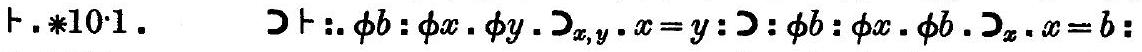
\includegraphics[max width=\textwidth, alt={}, center]{bc1848bf-39e8-4760-b069-9936044df683-055_52_1142_1045_145}\\
［＊533］$\supset: \phi b: \phi x . \nu_{x} . x=b$ ：\\
［＊13•191］\\
$\nu: x=b . \nu_{x} . \phi x$ ：

$$
\phi x \cdot \partial_{x} \cdot x=b:
$$

［＊10．22］


\begin{equation*}
\supset: \phi x . \equiv_{x} . x=b \tag{2}
\end{equation*}


ト ．（2）．$* 10 \cdot 1 \cdot 28 . \supset$ ：：（ H $^{b}$ ）：$\phi b: \phi x . \phi y . \supset_{x, y}, x=y: \supset:\left(y^{b}\right): \phi x . \equiv_{x} . x=b:$.\\
［＊10＊35］\\
ɔ $::\left(\right.$ H $\left.^{b}\right), \phi b: \phi x, \phi y, \partial_{x, y}, x=y: \partial:(\mathbb{H}): \phi x . \equiv_{x} . x=b:$\\
［＊14•11］


\begin{equation*}
\supset: \mathrm{E}!(x x)(\phi x) \tag{3}
\end{equation*}


ト．（1）．（3）．ɔ…Prop\\
＊14：204． । ： $\mathrm{E}!(n x)(\phi x) \cdot \equiv:\left(H^{b}\right) \cdot(n x)(\phi x)=b$\\
Dem．


\begin{align*}
& \vdash \cdot * 14 \cdot 202 \cdot * 10 \cdot 11 . \supset \\
& \vdash: .(b): . \phi x . \equiv_{x} \cdot x=b: \equiv:(1 x)(\phi x)=b: . \supset \\
& {[* 10 \cdot 281] \vdash:(\mathrm{H} b): \phi x . \equiv_{x} \cdot x=b: \equiv:(\mathrm{H} b) .(1 x)(\phi x)=b}  \tag{1}\\
& \vdash .(1) \cdot * 14 \cdot 11 . \supset \vdash . \text { Prop }
\end{align*}


＊14205．$\vdash: \psi(\omega x)(\phi x) \cdot \equiv \cdot\left(\mathrm{H}^{b}\right) \cdot b=(\omega x)(\phi x) \cdot \psi b[* 14 \cdot 202 \cdot 1]$\\
＊14：21．$\vdash: \psi(\boldsymbol{w} \boldsymbol{x})(\phi \boldsymbol{x})$ ．ɔ ．E！$(\boldsymbol{w} \boldsymbol{x})(\phi \boldsymbol{x})$\\
Dem．

$$
\begin{array}{ll}
\vdash \cdot * 14 \cdot 1 . \supset & \\
\vdash: \cdot \psi\{(1 x)(\phi x)\} . \supset:\left(\mathrm{H}^{b}\right): \phi x . \equiv_{x} \cdot x=b: \psi b: \\
{[* 10 \cdot 5]} & \supset:\left(\mathrm{H}^{b}\right): \phi x . \Xi_{x} \cdot x=b: \\
{[* 14 \cdot 11]} & \supset: \mathrm{E}!(1 x)(\phi x): . \text { つf. Prop }
\end{array}
$$

This proposition shows that if any true statement can be made about $(n x)(\phi x)$ ，then $(n x)(\phi x)$ must exist．Its use throughout the remainder of the work will be very frequent．

When $(n x)(\phi x)$ does not exist，there are still true propositions in which ＂$(h x)(\phi x)$＂occurs，but it has，in such propositions，a secondary occurrence， in the sense explained in Chapter III of the Introduction，i．e．the asserted proposition concerned is not of the form $\psi(x x)(\phi x)$ ，but of the form $f\{\psi(x x)(\phi x)\}$ ，in other words，the proposition which is the scope of $(x x)(\phi x)$ is only part of the whole asserted proposition．\\
＊14．22．$\vdash: \mathrm{E}!(x x)(\phi x) . \equiv . \phi(x x)(\phi x)$\\
Dem．\\
ト．＊14．122．ɔト：．$\phi x . \equiv_{x} . x=b:$ ɔ．$\phi b$\\
$\vdash .(1) . * 471 . \supset \vdash: . \phi x . \equiv_{x} . x=b: \equiv: \phi x . \equiv_{x} . x=b: \phi b:$.\\
$[* 10 \cdot 11 \cdot 281]$ ว ：：$\left(\mathrm{G}^{b}\right): \phi x . \equiv_{x} . x=b: \equiv:\left(\mathrm{G}^{b}\right): \phi x . \equiv_{x} . x=b: \phi b:$.\\
$[* 14 \cdot 11 \cdot 101] \quad$ つ $: \mathrm{E}!(n x)(\phi x) . \equiv . \phi(n x)(\phi x):$ ɔ ．Prop\\
As an instance of the above proposition，we may take the following：＂The proposition＇the author of Waverley existed＇is equivalent to＇the man who wrote Waverley wrote Waverley．＇＂Thus such a proposition as＂the man who wrote Waverley wrote Waverley＂does not embody a logically necessary truth，since it would be false if Waverley had not been written，or had been written by two men in collaboration．For example，＂the man who squared the circle squared the circle＂is a false proposition．\\
＊1423．$\vdash: \mathrm{E}!(n x)(\phi x \cdot \psi x)=\equiv \phi\{(n x)(\phi x \cdot \psi x)\}$\\
Dem．\\
ト．$* 1422$. つ $: . \mathrm{E}!(x x)(\phi x . \psi x)$ ．\\
［＊10．5．＊3．26］


\begin{equation*}
\equiv:[(h x)(\phi x \cdot \psi x)]: \phi\{(h x)(\phi x \cdot \psi x)\} \cdot \psi\{(h x)(\phi x \cdot \psi x)\} \tag{1}
\end{equation*}


$\vdash . * 14: 21$. つ $: \phi\{(1 x)(\phi x . \psi x)\}$. ɔ ．E ！$(1 x)(\phi x . \psi x)$

ト．（1）．（2）．ɔ. Prop\\
Note that in the second line of the above proof $* 10 \cdot 5$ ，not only $* 3 \cdot 26$ ，is required．For the scope of the descriptive symbol $(n x)(\phi x \cdot \psi x)$ is the whole product $\phi\{(x x)(\phi x \cdot \psi x)\} \cdot \psi\{(x x)(\phi x \cdot \psi x)\}$ ，so that，applying $* 14 \cdot 1$ ，the proposition on the right in the first line becomes

$$
(G b): \phi x \cdot \psi x \cdot \equiv_{x} \cdot x=b: \phi b \cdot \psi b
$$

which，by $* 10.5$ and $* 3 \cdot 26$ ，implies

$$
\begin{array}{lc} 
& \left(\mathrm{H}^{b}\right): \\
i . e . & \phi x \cdot \psi x \cdot \equiv_{x} \cdot x=b: \phi b \\
& \phi\{(n x)(\phi x \cdot \psi x)\} .
\end{array}
$$

＊1424．$\vdash: . \mathrm{E}!(y x)(\phi x) . \equiv:[(y x)(\phi x)]: \phi y . \equiv_{y \cdot y}=(1 x)(\phi x)$\\
Dem．\\
$\vdash . * 14 \cdot 1$. つ $\vdash: .[(n x)(\phi x)]: \phi y . \equiv_{y \cdot y=(n x)(\phi x):}$

$$
\equiv:\left(\mathrm{A}^{b}\right): \phi y \cdot \equiv_{y} \cdot y=b: \phi y \cdot \equiv_{y} \cdot y=b:
$$

SECTION B］\\
$[* 4 \cdot 24 \cdot * 10 \cdot 281]$\\
［＊14•11］

This proposition should be compared with $* 14 \cdot 241$ ，where，in virtue of the smaller scope of $(x)(\phi x)$ ，we get an implication instead of an equivalence．\\
＊14：241．$\vdash: . \mathrm{E}!(\boldsymbol{a} \boldsymbol{x})(\boldsymbol{\phi} \boldsymbol{x}) . \boldsymbol{\partial}: \phi y . \equiv_{y .} y=(\boldsymbol{\imath} \boldsymbol{x})(\phi \boldsymbol{x})$\\
Dem．

$$
\begin{aligned}
& \text { ト. } * 14: 203 . \text { つ }:: \mathrm{Hp} . \text { ɔ }: \phi y . \phi x . \text { ɔ } . y=x: . \\
& \text { [Exp] ɔ:. } \phi y . \supset: \phi x . \supset . y=x:: \\
& {[* 10 \cdot 11 \cdot 21] \supset \vdash:: \mathrm{Hp} . \supset: \phi y . \supset: \phi x . \partial_{x} . y=x: .} \\
& \text { [*4.71] } \quad \supset: . \phi y . \equiv: \phi y: \phi x . \partial_{x} . y=x: \\
& {[* 13 \cdot 191] \quad \equiv: y=x . \nu_{x} \cdot \phi x: \phi x . \nu_{x} \cdot y=x:} \\
& \text { [*10.22] } \equiv: \phi x . \equiv_{x} . y=x \text { : } \\
& \text { [*14:202] } \equiv: y=(x)(\phi x):: \text { つ } \text { । } \text { Prop }
\end{aligned}
$$

$$
\begin{aligned}
& \equiv:\left(\mathrm{H}^{b}\right): \phi y \cdot \equiv_{y} \cdot y=b: \\
& \equiv: \mathrm{E}!(n x)(\phi x): . \supset \vdash . \dot{\text { Prop }}
\end{aligned}
$$

＊14271．$\vdash:, \phi x . \equiv_{x}, \psi x: \supset: \mathrm{E}!(n x)(\phi x) . \equiv . \mathrm{E}!(n x)(\psi x)$\\
Dem．\\
ト．＊4：86．$\supset \vdash:: \phi x \equiv \psi x . \supset: . \phi x . \equiv . x=b: \equiv: \psi x . \equiv . x=b::$\\
$[* 10 \cdot 11 \cdot 27]$ つ $:: \mathrm{Hp}$ ．J：．$(x): . \phi x . \equiv . x=b: \equiv: \psi x . \equiv . x=b:$.\\
［＊10－271］ɔ：．$(x): \phi x . \equiv . x=b: \equiv:(x): \psi x . \equiv . x=b::$\\
$[* 10 \cdot 11 \cdot 21] \supset \vdash:: \mathrm{Hp} . \quad \supset: .(b): . \phi x . \equiv_{x} . x=b: \equiv: \psi x . \equiv_{x} . x=b:$.\\
［＊10．281］$\quad$ J：（ H $^{b}$ ）$: \phi x . \equiv_{x} . x=b: \equiv:\left(\right.$ H $\left.^{b}\right): \psi x . \equiv_{x} . x=b::$\\
ɔㄴ．Prop\\
＊14：272．$\vdash: . \phi x . \equiv_{x} . \psi x: \supset: \chi(h x)(\phi x) . \equiv . \chi(h x)(\psi x)$\\
Dem．\\
ト．＊4：86．$\supset \vdash:: \phi x \equiv \psi x . \supset: \phi x . \equiv . x=b: \equiv: \psi x . \equiv . x=b:$.\\
$[* 10 \cdot 11 \cdot 414] \supset f:: \mathrm{Hp} . \quad$ J ：$\phi x . \equiv_{x} . x=b: \equiv: \psi x . \equiv_{x} . x=b:$.\\
［Fact］ $2: \phi x . \equiv_{x} . x=b: \chi^{b}: \equiv: \psi x . \equiv_{x} . x=b: \chi^{b}:$ ．\\
$[* 10 \cdot 11 \cdot 21]$ ɔ ：：Hp．ɔ：．（b）：$\phi x . \equiv_{x} . x=b: \chi^{b}: \equiv: \psi x . \equiv_{x} . x=b: \chi^{b}:$.\\
［＊10．281］$\quad$ ：$\left(\right.$ H $\left.^{b}\right): \phi x . \equiv_{x} . x=b: \chi^{b}: \equiv$\\
［＊14：101］

$$
\supset: \cdot \chi(h x)(\phi x)=\equiv \cdot \chi \begin{gathered}
:\left(H^{b}\right): \psi x \cdot \Xi_{x} \cdot x=b: \chi \\
(h x)(\psi x):: \supset \vdash \cdot \text { Prop }
\end{gathered}
$$

The above two propositions show that $\mathbf{E}!(x x)(\phi x)$ and $\chi(x x)(\phi x)$ are ＂extensional＂properties of $\phi \hat{x}$ ，i．e．their truth－value is unchanged by the substitution，for $\phi \hat{x}$ ，of any formally equivalent function $\psi \hat{x}$ ．\\
＊14：28．$\vdash: \mathrm{E}!(x x)(\phi x) . \equiv .(x x)(\phi x)=(x x)(\phi x)$\\
Dem．\\
卜．$* 13 \cdot 15 \cdot * 4 \cdot 73$. つト $: \phi x . \equiv_{x} . x=b: \equiv: \phi x . \equiv_{x} . x=b: b=b$

ト．（1）．＊10．11．281．ɔ


\begin{equation*}
\vdash:\left(y^{b}\right): \phi x . \equiv_{x} \cdot x=b: \equiv:\left(y^{b}\right): \phi x . \equiv_{x} \cdot x=b: b=b \tag{1}
\end{equation*}


ト．（2）．＊14．1•11．）．Prop\\
This proposition states that $(\eta x)(\phi x)$ is identical with itself whenever it exists，but not otherwise．Thus for example the proposition＂the present King of France is the present King of France＂is false．

The purpose of the following propositions is to show that，when $E!(x x)(\phi x)$ ， the scope of $(1 x)(\phi x)$ does not matter to the truth－value of any proposition in which $(1 x)(\phi x)$ occurs．This proposition cannot be proved generally，but it can be proved in each particular case．The following propositions show the method，which proceeds always by means of $* 14 \cdot 242, * 10 \cdot 23$ and $* 14 \cdot 11$ ． The proposition can be proved generally when $(x x)(\phi x)$ occurs in the form $\chi(i x)(\phi x)$ ，and $\chi(i x)(\phi x)$ occurs in what we may call a＂truth－function，＂i．e． a function whose truth or falsehood depends only upon the truth or falsehood of its argument or arguments．This covers all the cases with which we are ever concerned．That is to say，if $\chi(1 x)(\phi x)$ occurs in any of the ways which can be generated by the processes of＊1—＊11，then，provided $\mathrm{E}!(x x)(\phi x)$ ， the truth－value of $f\{[(x x)(\phi x)] \cdot \chi(x x)(\phi x)\}$ is the same as that of

$$
[(h x)(\phi x)] \cdot f\{\chi(h x)(\phi x)\} .
$$

This is proved in the following proposition．In this proposition，however，the use of propositions as apparent variables involves an apparatus not required elsewhere，and we have therefore not used this proposition in subsequent proofs．\\
＊143．$\quad \vdash:, p \equiv q, \partial_{p, q} \cdot f(p) \equiv f(q): \mathrm{E}!(y x)(\phi x): \supset$ ：

$$
f\{[(x x)(\phi x)] \cdot \chi(y x)(\phi x)\} \cdot \equiv \cdot[(y x)(\phi x)] \cdot f\{\chi(y x)(\phi x)\}
$$

Dem．


\begin{align*}
& \text { ト.*14:242. ɔ } \\
& \vdash:, \phi x . \equiv_{x} . x=b: \mathcal{O}:[(n x)(\phi x)] \cdot \chi(n x)(\phi x) . \equiv . \chi^{b}  \tag{1}\\
& \vdash .(1) . \supset \vdash:, p \equiv q . \partial_{p, q} . f(p) \equiv f(q): \phi x . \equiv_{x} . x=b: \supset: \\
& f\{[(x x)(\phi x)] \cdot \chi(x x)(\phi x)\} \cdot \equiv \cdot f\left(\chi^{b}\right)  \tag{2}\\
& \text { ト.*14:242. ɔ } \\
& \vdash:, \phi x . \equiv_{x} . x=b: \omega:[(\imath x)(\phi x)] . f\{\chi(\imath x)(\phi x)\} . \equiv . f(\chi b)  \tag{3}\\
& \text { ト.(2).(3). ɔ } \\
& \text { + : } p \equiv q . \partial_{p, q} \cdot f(p) \equiv f(q): \phi x . \equiv_{x} \cdot x=b: \supset: \\
& f\{[(x x)(\phi x)] \cdot \chi(y x)(\phi x)\} \cdot \equiv \cdot[(y x)(\phi x)] \cdot f\{\chi(y x)(\phi x)\} \tag{4}
\end{align*}


ト．（4）．＊10．23．＊14．11．ɔ…Prop\\
The following propositions are immediate applications of the above．They are，however，independently proved，because $* 14 \cdot 3$ introduces propositions （ $p, q$ namely）as apparent variables，which we have not done elsewhere，and cannot do legitimately without the explicit introduction of the hierarchy of propositions with a reducibility－axiom such as $* 12 \cdot 1$ ．\\
＊1431． $\mathrm{F}:: \mathrm{E}!(n x)(\phi x) . \mathrm{J}:[(n x)(\phi x)] . p \vee \chi(n x)(\phi x)$.\\
Dem．

$$
\equiv: p \cdot \mathbf{v} \cdot[(\neg x)(\phi x)] \cdot \chi(\neg x)(\phi x)
$$

ト．$* 14 \cdot 242$. つ $: . \phi x . \equiv_{x} . x=b:$ ：$:[(1 x)(\phi x)] . p \vee \chi(1 x)(\phi x) . \equiv . p \vee \chi^{b}$


\begin{equation*}
\vdash . * 14242 . \supset \vdash: . \phi x . \equiv_{x} . x=b: \supset:[(x x)(\phi x)] \cdot \chi(1 x)(\phi x) . \equiv . \chi^{b}: \tag{1}
\end{equation*}


［＊4：37］


\begin{equation*}
\supset: p \mathbf{v}[(\neg x)(\phi x)] \chi(\neg x)(\phi x) . \equiv . p \mathbf{v} \chi^{b} \tag{2}
\end{equation*}


$\vdash .(1) .(2) . \supset \vdash: . \phi x . \equiv_{x} . x=b: \supset:[(1 x)(\phi x)] . p \vee \chi(1 x)(\phi x)$.


\begin{equation*}
\equiv . p \mathbf{v}[(\imath x)(\phi x)] \chi(\imath x)(\phi x) \tag{3}
\end{equation*}


ト．（3）．＊10．23．＊14．11．O 1. Prop\\
The following propositions are proved in precisely the same way as＊14．31； hence we shall merely give references to the propositions used in the proofs．\\
＊14：32． ！：． $\mathrm{E}!(x x)(\phi x) . \equiv:[(x x)(\phi x)] . \sim \chi(x x)(\phi x)$.

$$
\equiv \cdot \sim\{[(\imath x)(\phi x)] \cdot \chi(\imath x)(\phi x)\}
$$

$[* 14 \cdot 242 \cdot * 4 \cdot 11 \cdot * 10 \cdot 23 \cdot * 14 \cdot 11]$\\
The equivalence asserted here fails when $\sim \mathrm{E}!(x x)(\phi x)$ ．Thus，for example， let $\phi y$ be＂$y$ is King of France．＂Then $(n x)(\phi x)=$ the King of France．Let $\chi y$ be＂$y$ is bald．＂Then $[(n x)(\phi x)] \cdot \sim \chi(n x)(\phi x) \cdot=$ ．the King of France exists and is not bald；but $\sim\{[(x x)(\phi x)] \cdot \chi(x)(\phi x)\} .=$. it is false that the King of France exists and is bald．Of these the first is false，the second true．

Either might be meant by "the King of France is not bald," which is ambiguous ; but it would be more natural to take the first (false) interpretation as the meaning of the words. If the King of France existed, the two would be equivalent; thus as applied to the King of England, both are true or both false.\\
*1433. $\mathrm{F}:: \mathrm{E}!(x x)(\phi x) . \supset:[(x x)(\phi x)] . p \supset \chi(x x)(\phi x)$.

$$
\equiv: p \cdot \text { ɔ } \cdot[(\neg x)(\phi x)] \cdot \chi(\eta x)(\phi x)
$$

$[* 14 \cdot 242 \cdot * 4 \cdot 85 \cdot * 10 \cdot 23 \cdot * 14 \cdot 11]$\\
*14.331. $\dagger:: \mathrm{E}!(y x)(\phi x) . \supset:[(y x)(\phi x)] \cdot \chi(y x)(\phi x) \supset p$.

$$
\equiv:[(\imath x)(\phi x)] \cdot \chi(\imath x)(\phi x) \cdot \supset \cdot p
$$

$[* 4 \cdot 84 \cdot * 14 \cdot 242 \cdot * 10 \cdot 23 \cdot * 14 \cdot 11]$\\
*14.332. ' :: $\mathrm{E}!(\imath x)(\phi x) \cdot$ J : $[(\imath x)(\phi x)] \cdot p \equiv \chi(\imath x)(\phi x) \cdot \equiv$

$$
: p \cdot \equiv \cdot[(\neg x)(\phi x)] \cdot \chi(\neg x)(\phi x)
$$

$[* 4 \cdot 86 \cdot * 14 \cdot 242 \cdot * 10 \cdot 23 \cdot * 14 \cdot 11]$\\
*14:34. $\mathrm{F}:, p:[(h x)(\phi x)] \cdot \chi(h x)(\phi x): \equiv:[(h x)(\phi x)]: p \cdot \chi(h x)(\phi x)$\\
This proposition does not require the hypothesis $E!(x x)(\phi x)$.\\
Dem.\\
ト.*14:1.J\\
$\vdash:, p:[(\neg x)(\phi x)] \cdot \chi(x x)(\phi x): \equiv: p:\left(\mathrm{G}^{b}\right): \phi x \cdot \equiv_{x} \cdot x=b: \chi^{b}:$\\[0pt]
[*1035] $\equiv:\left(\mathrm{G}^{b}\right): p: \phi x . \equiv_{x} . x=b: \chi^{b}:$\\[0pt]
[*14-1] $\equiv:[(x x)(\phi x)]: p \cdot \chi(x x)(\phi x):$. ɔト.Prop\\
Propositions of the above type might be continued indefinitely, but as they are proved on a uniform plan, it is unnecessary to go beyond the fundamental cases of $p \vee q, \sim p, p \supset q$ and $p, q$.

It should be observed that the proposition in which $(x x)(\phi x)$ has the larger scope always implies the corresponding one in which it has the smaller scope, but the converse implication only holds if either $(a)$ we have $\mathbf{E}!(\boldsymbol{x} x)(\phi x)$ or (b) the proposition in which $(1 x)(\phi x)$ has the smaller scope implies $\mathbf{E}!(\pi x)(\phi x)$. The second case occurs in $* 14 \cdot 34$, and is the reason why we get an equivalence without the hypothesis $\mathbf{E}!(\boldsymbol{x} \boldsymbol{x})(\phi x)$. The proposition in which $(x x)(\phi x)$ has the larger scope always implies $E!(x x)(\phi x)$, in virtue of *14:21.

\section*{SECTION C}
\section*{CLASSES AND RELATIONS}
\section*{*20. GENERAL THEORY OF CLASSES}
\section*{Summary of $* 20$.}
The following theory of elasses, although it provides a notation to represent them, avoids the assumption that there are such things as classes. This it does by merely defining propositions in whose expression the symbols representing classes occur, just as, in $* 14$, we defined propositions containing descriptions.

The characteristics of a class are that it consists of all the terms satisfying some propositional function, so that every propositional function determines a class, and two functions which are formally equivalent (i.e. such that whenever either is true, the other is true also) determine the same class, while conversely two functions which determine the same class are formally equivalent. When two functions are formally equivalent, we shall say that they have the same extension. The incomplete symbols which take the place of classes serve the purpose of technically providing something identical in the case of two functions having the same extension; without something to represent classes, we cannot, for example, count the combinations that can be formed out of a given set of objects.

Propositions in which a function $\phi$ occurs may depend, for their truthvalue, upon the particular function $\phi$, or they may depend only upon the extension of $\phi$. In the former case, we will call the proposition concerned an intensional function of $\phi$; in the latter case, an extensional function of $\phi$. Thus, for example, $(x) \cdot \phi x$ or $\left(\mathrm{G}^{x}\right) \cdot \phi x$ is an extensional function of $\phi$, because, if $\phi$ is formally equivalent to $\psi$, i.e. if $\phi x \cdot \equiv_{x} \cdot \psi x$, we have $(x) \cdot \phi x \cdot \equiv \cdot(x) \cdot \psi x$ and $\left(H^{x}\right) \cdot \phi x \cdot \equiv \cdot\left(H^{x}\right) \cdot \psi x$. But on the other hand " I believe $(x) \cdot \phi x$ " is an intensional function, because, even if $\phi x \cdot \equiv_{x} \cdot \psi x$, it by no means follows that I believe $(x) \cdot \psi x$ provided I believe $(x) \cdot \phi x$. The mark of an extensional function $f$ of a function $\phi!\hat{z}$ is

$$
\phi!x \cdot \equiv_{x} \cdot \psi!x: \nu_{\phi, \psi}: f(\phi!\hat{z}) \cdot \equiv \cdot f(\psi!\hat{z}) .
$$

(We write " $\phi!\hat{z}$ " when we wish to speak of the function itself as opposed to its argument.) The functions of functions with which mathematics is specially concerned are all extensional.

When a function of $\phi!\hat{z}$ is extensional, it may be regarded as being about the class determined by $\phi!\hat{z}$, since its truth-value remains unchanged so long as the class is unchanged. Hence we require, for the theory of classes, a method of obtaining an extensional function from any given function of a function. This is effected by the following definition:\\
*2001. $f\{\hat{z}(\psi z)\} .=:($ H $\phi): \phi!x . \equiv_{x} . \psi x: f\{\phi!\hat{z}\} \quad$ Df\\
Here $f\{\hat{z}(\psi z)\}$ is in reality a function of $\psi \hat{z}$, which is defined whenever $f\{\phi!\hat{z}\}$ is significant for predicative functions $\phi!\hat{z}$. But it is convenient to regard $f\{\hat{z}(\psi z)\}$ as though it had an argument $\hat{z}(\psi z)$, which we will call "the class determined by the function $\psi \hat{z}$." It will be proved shortly that $f\{\hat{z}(\psi z)\}$ is always an extensional function of $\psi \hat{z}$, and that, applying the definition of identity (*13.01) to the fictitious objects $\hat{z}(\phi z)$ and $\hat{z}(\psi z)$, we have

$$
\hat{z}(\phi z)=\hat{z}(\psi z) \cdot \equiv:(x): \phi x \cdot \equiv \cdot \psi x .
$$

This last is the distinguishing characteristic of classes, and justifies us in treating $\hat{z}(\psi z)$ as the class determined by $\psi \hat{z}$.

With regard to the scope of $\hat{z}(\psi z)$, and to the order of elimination of two such expressions, we shall adopt the same conventions as were explained in *14 for $(1 x)(\phi x)$. The condition corresponding to

$$
E!(h x)(\psi x) \text { is }(H \phi): \phi!x \cdot \equiv_{x} \cdot \psi x
$$

which is always satisfied because of $* 12 \cdot 1$.\\
Following Peano, we shall use the notation

$$
x \in \hat{z}(\psi z)
$$

to express " $x$ is a member of the class determined by $\psi \hat{z}$." We therefore introduce the following definition:\\
*20.02. $x \in(\phi!\hat{z}) .=. \phi!x$ Df\\
In this form, the definition is never used; it is introduced for the sake of the proposition

$$
\vdash: . x \in \hat{z}(\psi z) . \equiv:(\mathcal{H} \phi): \psi y . \equiv_{y} . \phi!y: \phi!x
$$

which results from $* 20.02$ and $* 20.01$, and leads to

$$
\vdash: x \in \hat{z}(\psi z) \cdot \equiv \cdot \psi x
$$

by the help of $* 12 \cdot 1$.\\
We shall use small Greek letters (other than $\epsilon, \iota, \pi, \phi, \psi, \chi, \theta$ ) to represent classes, i.e. to stand for symbols of the form $\hat{z}(\phi z)$ or $\hat{z}(\phi!z)$. When a small Greek letter occurs as apparent variable, it is to be understood to stand for a symbol of the form $\hat{z}(\phi!z)$, where $\phi$ is properly the apparent variable concerned. The use of single letters in place of such symbols as $\hat{z}(\phi z)$ or $\hat{z}(\phi!z)$ is practically almost indispensable, since otherwise the notation rapidly becomes intolerably cumbrous. Thus " $x \in \alpha$ " will mean " $x$ is a member of the class $\alpha$," and may be used wherever no special defining function of the class $\alpha$ is in question.

The following definition defines what is meant by a class.

\section*{*20.03. $\mathrm{Cls}=\hat{\alpha}\{(\neg \phi) \cdot \alpha=\hat{z}(\phi!z)\} \quad \mathrm{Df}$}
Note that the expression " $\hat{\alpha}\{(\mathcal{H} \phi) \cdot \alpha=\hat{z}(\phi!z)\}$ " has no meaning in isolation: we have merely defined (in *20.01) certain uses of such expressions. What the above definition decides is that the symbol " Cls " may replace the symbol " $\hat{\alpha}\{(\mathcal{H} \phi) \cdot \alpha=\hat{z}(\phi!z)\}$," wherever the latter occurs, and that the\\
meaning of the combination of symbols concerned is to be unchanged thereby. Thus "Cls," also, has no meaning in isolation, but merely in certain uses.

The above definition, like many future definitions, is ambiguous as to type. The Latin letter $z$, according to our conventions, is to represent the lowest type concerned; thus $\phi$ is of the type next above this. It is convenient to speak of a class as being of the same type as its defining function; thus $\alpha$ is of the type next above that of $z$, and "Cls" is of the type next above that of $\alpha$. Thus the type of " Cls " is fixed relatively to the lowest type concerned; but if, in two different contexts, different types are the lowest concerned, the meaning of " Cls " will be different in these two contexts. The meaning of " Cls " only becomes definite when the lowest type concerned is specified.

Equality between classes is defined by applying *13.01, symbolically unchanged, to their defining functions, and then using $* 20.01$.

The propositions of the present number may be divided into three sets. First, we have those that deal with the fundamental properties of classes; these end with $* 20.43$. Then we have a set of propositions dealing with both classes and descriptions; these extend from $* 20.5$ to $* 20.59$ (with the exception of $* 20.53 .54$ ). Lastly, we have a set of propositions designed to prove that classes of classes have all the same formal properties as classes of individuals.

In the first set, the principal propositions are the following.\\
*20•15. F : $. \psi x . \equiv_{x} \cdot \chi^{x}: \equiv . \hat{z}(\psi z)=\hat{z}(\chi z)$\\
I.e. two classes are identical when, and only when, their defining functions are formally equivalent. This is the principal property of classes.\\
*2031. $\vdash:, \hat{z}(\psi z)=\hat{z}(\chi z) . \equiv: x \in \hat{z}(\psi z) . \equiv_{x} . x \in \hat{z}(\chi z)$\\
I.e. two classes are identical when, and only when, they have the same members.\\
*20.43. $\vdash: . \alpha=\beta . \equiv: x \in \alpha . \equiv_{x} . x \in \beta$\\
This is the same proposition as $* 2031$, merely employing Greek letters in place of $\hat{z}(\psi z)$ and $\hat{z}(\chi z)$.\\
*2018. $\vdash: . \hat{z}(\phi z)=\hat{z}(\psi z) . \supset: f\{\hat{z}(\phi z)\} . \equiv . f\{\hat{z}(\psi z)\}$\\
I.e. if two classes are identical, any property of either belongs also to the other. This is the analogue of *13.12.\\
*2022122, which prove that identity between classes is reflexive, symmetrical and transitive.\\
*203. $\vdash: x \in \hat{z}(\psi z) . \equiv . \psi x$\\
I.e. a term belongs to a class when, and only when, it satisfies the defining function of the class.

In the second set of propositions ( $* 20 \cdot 5-59$ ), we show that, under suitable circumstances, expressions such as $(1 x)(\phi x)$ may be substituted for $x$ in $* 203$\\
and various other propositions of the first set，and we prove a few properties of such expressions as＂$(1 \alpha)(f \alpha)$ ，＂i．e．＂the class which satisfies the function $f$ ．＂ Here it is to be remembered that＂$\alpha$＂stands for＂$\hat{z}(\phi z)$ ，＂and that＂$f \alpha$＂ therefore stands for＂$f\{\hat{z}(\phi z)\}$ ．＂This is，in reality，a function of $\phi \hat{z}$ ，namely the extensional function associated with $f(\psi!\hat{z})$ by means of $* 20 \cdot 01$ ．Thus an expression containing a variable class is always an abbreviation for an expression containing a variable function．

In the third set of propositions，we prove that variable classes satisfy all the primitive propositions assumed for variable individuals or functions，whence it follows，by merely repeating the proofs of the first set of propositions（ $* 20 \cdot 1$ －43），that classes of classes have all the formal properties of classes of in－ dividuals or functions．We shall never have occasion explicitly to consider classes of functions，but classes of classes will occur constantly－for example， every cardinal number will be defined as a class of classes．Classes of relations， which will also frequently occur，will be considered in $* 21$ ．\\
＊2001．$f\{\hat{z}(\psi z)\} .=:(\mathrm{H} \phi): \phi!x . \equiv_{x} . \psi x: f\{\phi!\hat{z}\}$ Df\\
＊20．02．$x \in(\phi!\hat{z}) .=. \phi!x \quad$ Df\\
＊20．03．Cls $=\hat{\alpha}\{($ 田 $\phi) \cdot \alpha=\hat{z}(\phi!z)\} \quad$ Df\\
The three following definitions serve merely for purposes of abbreviation．\\
＊20．04．$x, y \in \alpha .=. x \in \alpha . y \in \alpha \quad$ Df\\
＊2005．$x, y, z \in \alpha .=. x, y \in \alpha . z \in \alpha$ Df\\
＊20．06．$x \sim \epsilon$ α．$=. \sim(x \in \alpha) \quad$ Df\\
The following definitions merely extend to symbols representing classes the definitions which have already been given for other symbols，with the smallest possible modifications．\\
＊20．07．（ $\alpha$ ）．$f \alpha .=.(\phi) . f\{\hat{z}(\phi!z)\} \quad$ Df\\
＊20071．（马 $\alpha$ ）．$f \alpha .=.(\neg \phi) . f\{\hat{z}(\phi!z)\} \quad$ Df\\
＊20．072．$[(\nu \alpha)(\phi \alpha)] \cdot f(\nu \alpha) \cdot(\phi \alpha) \cdot=:($ 月 $\gamma): \phi \alpha . \equiv_{\alpha} \cdot \alpha=\gamma: f_{\gamma}$ Df\\
＊20．08．$f\{\hat{\alpha}(\psi \alpha)\} .=:(\psi \phi): \psi \alpha . \equiv_{\alpha} . \phi!\alpha: f(\phi!\hat{\alpha}) \quad$ Df\\
＊20．081．$\alpha \in \psi!\hat{\alpha} .=. \psi!\alpha \quad$ Df\\
The propositions which follow give the most general properties of classes．\\
＊20．1．$\vdash: . f\{\hat{z}(\psi z)\} . \equiv:(\mathrm{H} \phi): \phi!x . \equiv_{x} . \psi x: f\{\phi!\hat{z}\} \quad[* 4 \cdot 2 .(* 20 \cdot 01)]$\\
＊2011．$\vdash: . \psi x . \equiv_{x} \cdot \chi^{x}: \mathcal{J}: f\{\hat{z}(\psi z)\} \cdot \equiv \cdot f\{\hat{z}(\chi z)\}$\\
Dem．\\
$\vdash . * 486 . \supset \vdash:: \mathrm{Hp} . \supset: . \phi!x . \equiv_{x} . \psi x: \Xi_{\phi}: \phi!x . \equiv_{x} . \chi^{x}:$.\\
$[* 4: 36] \quad \supset: \phi!x . \equiv_{x} . \psi x: f\{\phi!\hat{z}\}: \equiv_{\phi}: \phi!x . \equiv_{x} \cdot \chi^{x}: f\{\phi!\hat{z}\}:$.\\
［＊10281］$\supset:(\mathrm{H} \phi): \phi!x ._{x-\psi x}: f\{\phi!\hat{z}\}:$\\
$\equiv:(\mathrm{H} \phi): \phi!x . \equiv_{x} \cdot \chi x: f\{\phi!\hat{z}\}:$.\\
$[* 20 \cdot 1]$\\
$\supset: . f\{\hat{z}(\psi z)\} . \equiv . f\{\hat{z}(\chi z)\}:: \supset \vdash$. Prop

This proves that every proposition about a class expresses an extensional property of the determining function of the class，and therefore does not depend for its truth or falsehood upon the particular function selected for determining the class，but only upon the extension of the determining function．\\
＊20•111．$\vdash: \cdot f(\phi!\hat{z}) . \equiv_{\phi} . g(\phi!\hat{z}): \supset: f\{\hat{z}(\phi!z)\} . \equiv_{\phi} . g\{\hat{z}(\phi!z)\}$\\
Dem．\\
$\vdash$. Fact．$\supset \vdash:: \mathrm{Hp} . \supset: . \phi!x . \equiv_{x} . \psi!x: f(\psi!\hat{z}): \equiv: \phi!x . \equiv_{x} . \psi!x: g(\psi!\hat{z}):: [* 10 \cdot 11 \cdot 21] \supset \vdash:: \mathrm{Hp} . \supset: . \phi!x . \equiv_{x} \cdot \psi!x: f(\psi!\hat{z}): \equiv_{\psi}: \phi!x . \equiv_{x} \cdot \psi!x: g(\psi!\hat{z}):$.\\
［＊10：281］つ：（H $\psi$ ）：$\phi!x . \equiv_{x} \psi!x: f(\psi!\hat{z}): \equiv:(\mathrm{H} \psi): \phi!x . \equiv_{x} \cdot \psi!x: g(\psi!\hat{z}):$\\
$[* 20 \cdot 1] \quad$ J：．$f\{\hat{z}(\phi!x)\} . \equiv . g\{\hat{z}(\phi!x)\}$

ト．（1）．＊10．11．21．ɔ ．Prop\\
＊20－112．$\vdash: .(\mathrm{H} g): . f\{\hat{z}(\phi!z)\} . \equiv_{\phi} . g!\{\hat{z}(\phi!z)\}$\\
Dem．


\begin{align*}
& \vdash \cdot * 12 \cdot 1 . \supset \vdash: \cdot(\mathrm{H} g): f(\phi!\hat{z}) \cdot \equiv_{\phi} \cdot g!(\phi!\hat{z})  \tag{1}\\
& \vdash .(1) \cdot * 20 \cdot 111 . \supset \vdash . \text { Prop }
\end{align*}


Thus the axiom of reducibility still holds for classes as arguments．\\
＊2012． $\mathrm{F}:(\mathrm{H} \phi): \phi!x . \equiv_{x} \cdot \psi x: f\{\hat{z}(\psi z)\} . \equiv . f\{\hat{z}(\phi!z)\} \quad[* 2011 . * 121]$\\
＊20－13．$\vdash: . \psi x . \equiv_{x} \cdot \chi^{x}:$ つ．$\hat{z}(\psi z)=\hat{z}\left(\chi^{z}\right)$\\
The meaning of＂$\hat{z}(\psi z)=\hat{z}(\chi z)$＂is obtained by a double application of $* 20.01$ to $* 13.01$ ，remembering the convention that $\hat{z}(\psi z)$ is to have a larger scope than $\hat{z}\left(\chi^{z}\right)$ because it occurs first．

Dem．\\
$\vdash \cdot * 201 . \supset \vdash:: \hat{z}(\psi z)=\hat{z}(\chi z) \cdot \equiv: \cdot(\mathbb{H} \phi): \psi x . \equiv_{x} \cdot \phi!x: \phi!\hat{z}=\hat{z}(\chi z):$.\\
［＊20•1］


\begin{equation*}
\equiv: .(\mathrm{H} \phi, \theta): . \psi x . \equiv_{x} . \phi!x: \chi x . \equiv_{x} . \theta!x: \phi!\hat{z}=\theta!\hat{z} \tag{1}
\end{equation*}


ト．＊121．＊10321．つ\\
F ：：Hp．J：．$(H \phi): \psi x . \equiv_{x} . \phi!x: \chi x . \Xi_{x} . \phi!x:$.\\
$[* 13 \cdot 195]$ ：$($ H $\phi, \theta): . \psi x . \equiv_{x} \cdot \phi!x: \chi^{x} . \equiv_{x} \cdot \theta!x: \phi!\hat{z}=\theta!\hat{z}$

F．（1）．（2）．ɔㄴ．Prop\\
＊20－14．$\vdash: . \hat{z}(\psi z)=\hat{z}\left(\chi^{z}\right) \cdot \supset: \psi x \cdot \equiv_{x} \cdot \chi^{x}$\\
Dem．\\
$\vdash . * 201 . \supset \vdash:: \hat{z}(\psi z)=\hat{z}(\chi z) . \equiv: .(H \phi): \psi x . \equiv_{x} . \phi!x: \phi!\hat{z}=\hat{z}(\chi z):$.\\
$[* 20 \cdot 1] \quad \equiv:(\mathrm{H} \phi, \theta): . \psi x . \equiv_{x} . \phi!x: \chi x . \equiv_{x} . \theta!x: \phi!\hat{z}=\theta!\hat{z}:$.\\
$[* 13 \cdot 195] \equiv: \cdot(\mathrm{H} \phi): . \psi x . \equiv_{x} . \phi!x: \chi^{x} . \equiv_{x} . \phi!x:$.\\
［＊10．322］D：．$\psi x . \equiv_{x} . \chi^{x}::$ J＋．Prop\\
This proposition is the converse of $* 20 \cdot 13$ ．\\
＊20•15．$\dagger: . \psi x . \equiv_{x} \cdot \chi^{x: \equiv .} \hat{z}(\psi z)=\hat{z}\left(\chi^{z}\right) \quad[* 20 \cdot 13 \cdot 14]$\\
This proposition states that two functions determine the same class when， and only when，they are formally equivalent，i．e．are satisfied by the same set of values．This is the essential property of classes，and gives the justification of the definition $* 20.01$ ．\\
＊20151． ᄀ ．$(\mathrm{H} \phi)$ ．$\hat{z}(\psi z)=\hat{z}(\phi!z)$\\
Dem．\\
ト．＊2015．つト：$\psi x . \equiv_{x} . \phi!x: \supset . \hat{z}(\psi z)=\hat{z}(\phi!z):$.


\begin{equation*}
[* 10 \cdot 11 \cdot 28] \quad \supset \vdash:(H \phi): \psi x . \equiv_{x} . \phi!x: \supset .(H \phi) . \hat{z}(\psi z)=\hat{z}(\phi!z) \tag{1}
\end{equation*}


ト．（1）．＊121．ɔ. Prop\\
In virtue of this proposition，all classes can be obtained from predicative functions．This fact is especially important when classes are used as apparent variables．For in that case，according to the definitions $* 20.07 .071$ ，the ap－ parent variable really involved is a predicative function．In virtue of $* 20 \cdot 151$ ， this places no limitation upon the classes concerned，except the limitation which inevitably results from the nature of their membership．A class，there－ fore，unlike a function，has its order completely determined by the order of its possible members，i．e．of the arguments which render its defining function significant．\\
＊20．16． $\mathrm{F}:(\mathrm{H} \phi): f\{\widehat{\mathrm{~s}}(\psi z)\} . \equiv . f\{\widehat{\mathrm{z}}(\phi!z)\} \quad$［＊20．12］\\
＊20．17．$\vdash:(\phi) \cdot f\{\hat{z}(\phi!z)\} \cdot$ J．$f\{\hat{z}(\psi z)\} \quad[* 20 \cdot 16 \cdot * 10 \cdot 1]$\\
＊20•18．$\vdash: . \hat{z}(\phi z)=\hat{z}(\psi z) . \supset: f\{\hat{z}(\phi z)\} . \equiv . f\{\hat{z}(\psi z)\}[* 20 \cdot 11 \cdot 15]$\\
＊20－19．$\vdash: . \hat{z}(\psi z)=\hat{z}(\chi z) . \equiv:(f): f!\hat{z}(\psi z) . \supset . f!\hat{z}(\chi z)$\\
Dem．\\
ト ．$* 20 \cdot 18 . * 10 \cdot 11 \cdot 21$. つ $\vdash: \hat{z}(\psi z)=\hat{z}(\chi z)$. ɔ ：


\begin{equation*}
(f): f!\hat{z}(\psi z) \cdot \supset \cdot f!\hat{z}(\chi z) \tag{1}
\end{equation*}


$\vdash . * 20 \cdot 18 \cdot 15 . \supset \vdash:: \phi!x . \equiv_{x} \cdot \psi x: \theta!x . \equiv_{x} \cdot \chi^{x}: f!\hat{z}(\psi z) \cdot \supset \cdot f!\hat{z}(\chi z): \supset:$


\begin{equation*}
f!\hat{z}(\phi!z) \cdot \supset \cdot f!\hat{z}(\theta!z) \tag{2}
\end{equation*}


ト．（2）．＊10．11．27．33．ɔ\\
$\vdash:: \phi!x . \equiv_{x} . \psi x: \theta!x . \equiv_{x} . \chi^{x}: .(f): f!\hat{z}(\psi z) . \supset . f!\hat{z}(\chi z): . \supset:$.

$$
(f): f!\hat{z}(\phi!z) \cdot \supset \cdot f!\hat{z}(\theta!z): .
$$

$[* 20 \cdot 112 \cdot * 10 \cdot 1] ~ \supset: . \phi!x . \equiv_{x} . \phi!x: \supset: \phi!x . \equiv_{x} . \theta!x:$.\\
［＊4•2］ɔ：．$\phi!x . \equiv_{x} . \theta!x:$.\\
$[* 10 \cdot 301 \cdot 32 . \mathrm{Hp}]$ つ $: \psi x . \equiv_{x} \cdot \chi^{x}:$.\\
［＊20．15］つ：．$\hat{z}(\psi z)=\hat{z}(\chi z)$

ト．（3）．＊10．11．23．35．）\\
$\vdash::($ 田 $\phi, \theta): \phi!x . \equiv_{x} \cdot \psi x: \theta!x . \equiv_{x} \cdot \chi^{x}: .(f): f!\hat{z}(\psi z)$. ɔ $. f!\hat{z}\left(\chi^{z}\right):$.


\begin{equation*}
\text { ɔ. } \hat{z}(\psi z)=\hat{z}(\chi z) \tag{4}
\end{equation*}


ト．（4）．$* 12 \cdot 1$. つト：$(f): f!\hat{z}(\psi z)$. ɔ．$f!\hat{z}(\chi z):$ ɔ．$\hat{z}(\psi z)=\hat{z}(\chi z)$

ト．（1）．（5）．ɔ‥Prop\\
＊20－191．$+: . \hat{z}(\psi z)=\hat{z}(\chi z) . \equiv:(f): f!\hat{z}(\psi z) . \equiv . f!\hat{z}(\chi z)$\\
$[* 20 \cdot 18 \cdot 19 \cdot * 10 \cdot 22]$\\
＊202． F．$\hat{z}(\phi z)=\hat{z}(\phi z)$\\
Dem．


\begin{equation*}
\vdash \cdot * 20 \cdot 15 . \supset \vdash: . \hat{z}(\phi z)=\hat{z}(\phi z) \cdot \equiv: \phi x \cdot \equiv_{x} \cdot \phi x \tag{1}
\end{equation*}


ト．（1）．＊42．＊10．11．つト．Prop\\
＊2021．$F: \hat{z}(\phi z)=\hat{z}(\psi z) . \equiv . \hat{z}(\psi z)=\hat{z}(\phi z) \quad[* 20 \cdot 15 . * 10 \cdot 32]$\\
＊2022．$\vdash: \hat{z}(\phi z)=\hat{z}(\psi z) \cdot \hat{z}(\psi z)=\hat{z}(\chi z) \cdot \supset \cdot \hat{z}(\phi z)=\hat{z}(\chi z)$\\
［ $* 20 \cdot 15 \cdot * 10 \cdot 301$ ］\\
The above propositions are not immediate consequences of $* 13 \cdot 15 \cdot 16 \cdot 17$ ， for a reason analogous to that explained in the note to $* 14 \cdot 13$ ，namely because $f\{\hat{z}(\phi z)\}$ is not a value of $f x$ ，and therefore in particular＂$\hat{z}(\phi z)=\hat{z}(\psi z)$＂is not a value of＂$x=y$ ．＂\\
＊20．23．$\vdash: \hat{z}(\phi z)=\hat{z}(\psi z) \cdot \hat{z}(\phi z)=\hat{z}(\chi z) \cdot$ J．$\hat{z}(\psi z)=\hat{z}(\chi z) \quad[* 20 \cdot 21 \cdot 22]$\\
＊2024．$\vdash: \hat{z}(\psi z)=\hat{z}(\phi z) \cdot \hat{z}(\chi z)=\hat{z}(\phi z) \cdot$ J．$\hat{z}(\psi z)=\hat{z}(\chi z) \quad[* 20 \cdot 21 \cdot 22]$\\
＊2025． $\mathrm{F}: . \alpha=\hat{z}(\phi z) . \equiv_{a} . \alpha=\hat{z}(\psi z): \equiv . \hat{z}(\phi z)=\hat{z}(\psi z)$\\
Dem．\\
ト．$* 10 \cdot 1 . \quad \supset \vdash: \alpha=\hat{z}(\phi z) \cdot \equiv_{\alpha} \cdot \alpha=\hat{z}(\psi z): \supset$ ：\\
［＊20•2］


\begin{gather*}
\hat{z}(\phi z)=\hat{z}(\phi z) \cdot \equiv \cdot \hat{z}(\phi z)=\hat{z}(\psi z): \\
\supset: \hat{z}(\phi z)=\hat{z}(\psi z) \tag{1}
\end{gather*}


ト．$* 2022$ ．$\supset \vdash: \alpha=\hat{z}(\phi z) \cdot \hat{z}(\phi z)=\hat{z}(\psi z) \cdot \supset \cdot \alpha=\hat{z}(\psi z):$\\
［Exp．Comm］$\supset \vdash: \hat{z}(\phi z)=\hat{z}(\psi z) \cdot \supset: \alpha=\hat{z}(\phi z) \cdot \supset \cdot \alpha=\hat{z}(\psi z)$

ト ．＊2024．$\supset \vdash:, \hat{z}(\phi z)=\hat{z}(\psi z) \cdot \alpha=\hat{z}(\psi z) \cdot \supset \cdot \alpha=\hat{z}(\phi z)$ ：．\\
［Exp］$\supset \vdash: \hat{z}(\phi z)=\hat{z}(\psi z) . \supset: \alpha=\hat{z}(\psi z) . \supset . \alpha=\hat{z}(\phi z)$

ト．（2）．（3）．$\supset \vdash: \hat{z}(\phi z)=\hat{z}(\psi z) \cdot \supset: \alpha=\hat{z}(\phi z) \cdot \equiv \cdot \alpha=\hat{z}(\psi z):$.


\begin{equation*}
[* 10 \cdot 11 \cdot 21] \quad \supset \vdash: \hat{z}(\phi z)=\hat{z}(\psi z) \cdot \supset: \alpha=\hat{z}(\phi z) \cdot \equiv_{\alpha} \cdot \alpha=\hat{z}(\psi z) \tag{3}
\end{equation*}


ト．（1）．（4）．ɔ…Prop\\
＊203．$\vdash: x \in \hat{z}(\psi z) . \equiv . \psi x$\\
Dem．

$$
\begin{aligned}
& \text { F. } * 20 \cdot 1 . \supset \\
& \vdash:: x \in \hat{z}(\psi z) . \equiv: .(\mathrm{H} \phi): . \psi y . \equiv_{v} . \phi!y: x \in(\phi!\hat{z}): . \\
& {[(* 20 \cdot 02)] \quad \equiv: .(\mathrm{H} \phi): . \psi y . \equiv_{y} . \phi!y: \phi!x: .} \\
& {[* 10 \cdot 43] \quad \equiv: .(\mathrm{H} \phi): \psi y . \equiv_{y} . \phi!y: \psi x: .} \\
& {[* 10 \cdot 35] \quad \equiv:(\mathrm{H} \phi): \psi y . \equiv_{y} . \phi: y: \psi x: .} \\
& {[* 12 \cdot 1] \quad \equiv: \psi x: \text { J . Prop }}
\end{aligned}
$$

This proposition shows that $x$ is a member of the class determined by $\psi$ when，and only when，$x$ satisfies $\psi$ ．\\
＊2031．\\
＊2032．

$$
\vdash: . \hat{z}(\psi z)=\hat{z}(\chi z) . \equiv: x \in \hat{z}(\psi z) . \equiv_{x} . x \in \hat{z}(\chi z) \quad[* 20 \cdot 15 \cdot 3]
$$

ト．$\hat{x}\{x \in \hat{z}(\phi z)\}=\hat{z}(\phi z)$\\
［＊20．3．15］\\
＊2033．

$$
F: \alpha=\hat{z}(\phi z) . \equiv: x \in \alpha . \equiv_{x} \cdot \phi x
$$

Dem．


\begin{align*}
& \vdash \cdot * 2031 . \quad \supset \vdash: . \alpha=\hat{z}(\phi z) . \equiv: x \in \alpha . \equiv_{x} . x \in \hat{z}(\phi z)  \tag{1}\\
& \vdash .(1) \cdot * 203 . \supset \vdash . \text { Prop }
\end{align*}


Here $\alpha$ is written in place of some expression of the form $\hat{z}(\psi z)$ ．The use of the single Greek letter is more convenient whenever the determining function is irrelevant．\\
＊2034．$\vdash: . x=y . \equiv: x \in \alpha . \partial_{\alpha}, y \in \alpha$\\
Dem．

$$
\begin{aligned}
\vdash . * 4 \cdot 2 .(* 20 \cdot 07) . \supset \vdash: . x \in \alpha . \partial_{\alpha} . y \in \alpha: & \equiv: x \in \hat{z}(\phi!z) . \partial_{\phi} . y \in \hat{z}(\phi!z): \\
& \equiv: \phi!x . \partial_{\phi} . \phi!y: \\
{[* 20 \cdot 3] } & \equiv: x=y: . \supset \vdash . \text { Prop }
\end{aligned}
$$

The above proposition and $* 20.25$ illustrate the use of Greek letters as apparent variables．

\[
\begin{array}{ll}
\vdash: x=y . \equiv: x \in \alpha . \equiv_{\alpha} . y \in \alpha & {[* 20.3 . * 13.11]}  \tag{*2035.}\\
\vdash: \alpha \in \mathrm{Cls} . \equiv .(\mathrm{H} \phi) . \alpha=\widehat{z}(\phi!z) & {[* 20.3 .(* 20.03)]} \\
\vdash . \hat{z}(\psi z) \in \mathrm{Cls} & {[* 20.4 \cdot 151]}
\end{array}
\]

＊204．\\
＊2042．

$$
\vdash . \hat{z}(z \in \alpha)=\alpha
$$

A Greek letter，such as $\alpha$ ，is merely an abbreviation for an expression of the form $\hat{z}(\phi z)$ ；thus this proposition is $* 20.32$ repeated．

Dem．

$$
\begin{aligned}
& \vdash . * 20 \cdot 3 . * 10 \cdot 11 . \text { コト }: x \in \hat{z}(\psi z) . \equiv_{x} \cdot \psi x: \\
& {[* 20 \cdot 15] \quad \text { コト. } \hat{x}\{x \in \hat{z}(\psi z)\}=\hat{x}(\psi x) . \text { ɔ } . \text { Prop }}
\end{aligned}
$$


\begin{equation*}
\vdash: \alpha=\beta . \equiv: x \in \alpha . \equiv_{x} . x \in \beta \quad[* 2031] \tag{$* 2043$.}
\end{equation*}


The following propositions deal with cases in which both classes and descriptions occur．In such cases，we shall，in the absence of any indication to the contrary，adopt the convention that the descriptions are to have a larger scope than the classes，in applying the definitions $* 14.01$ and $* 20.01$ ．\\
＊20．5．$\vdash:(n x)(\phi x) \in \hat{z}(\psi z) . \equiv . \psi\{(n x)(\phi x)\}$\\
Dem．

$$
\begin{array}{ll}
\vdash \cdot * 14 \cdot 1 . \supset \vdash::(1 x)(\phi x) \in \hat{z}(\psi z) . \equiv: .(\mathrm{H} c): \phi x . \equiv_{x}: x=c: c \in \hat{z}(\psi z): . \\
\begin{array}{ll}
{[* 20 \cdot 3]} & \equiv:\left(\mathrm{H}^{c)}: \phi x . \equiv_{x}: x=c: \psi c: .\right. \\
{[* 14 \cdot 1]} & \equiv: \psi\{(1 x)(\phi x)\}:: \supset \vdash . \text { Prop }
\end{array}
\end{array}
$$

＊2051．$\vdash:(h x)(\phi x)=b . \equiv:(h x)(\phi x) \in \alpha . \equiv_{\alpha} . b \in \alpha$\\
Dem．\\
ト ．$* 205 \cdot 3$. つ

$$
\begin{aligned}
& \vdash:(1 x)(\phi x) \in \hat{z}(\psi!z) . \equiv . b \in \hat{z}(\psi!z): \equiv: \psi!(1 x)(\phi x) . \equiv . \psi!b: . \supset \\
& {[* 10 \cdot 11] \vdash: .(1 x)(\phi x) \in \alpha . \equiv_{\alpha} . b \in \alpha: \equiv: \psi!(1 x)(\phi x) . \equiv_{\psi} . \psi!b:} \\
& {[* 14 \cdot 17] \quad \equiv:(1 x)(\phi x)=b: . \supset \vdash . \text { Prop }}
\end{aligned}
$$

＊2052．$\vdash: \mathrm{E}!(7 x)(\phi x) . \equiv:\left(\mathrm{H}^{b}\right):(1 x)(\phi x) \in \alpha . \equiv_{\alpha} . b \in \alpha$\\
Dem．


\begin{align*}
& \text { ト. } * 20.51 \cdot * 10 \cdot 11 \cdot 281 . \supset \\
& \text { 卜:. }(\mathrm{H} b) \cdot(1 x)(\phi x)=b \cdot \equiv:(\mathrm{H} b):(1 x)(\phi x) \in \alpha \cdot \equiv_{a} \cdot b \in \alpha  \tag{1}\\
& \text { 卜. }(1) \cdot * 14 \cdot 204 . \supset \text {. Prop }
\end{align*}


$* 20.53 . \vdash: . \beta=\alpha . \partial_{\beta} . \phi \beta: \equiv . \phi \alpha$\\
This is the analogue of $* 13 \cdot 191$ ．

Dem．


\begin{align*}
& \text { ト. } * 10 \cdot 1 . \quad \supset \vdash:, \beta=\alpha . \partial_{\beta} . \phi \beta: \partial: \alpha=\alpha . \supset . \phi \alpha: \\
& \text { [*20.2] ɔ:φα }  \tag{1}\\
& \text { ト . } * 20 \text { 18-21. } \text { つ }: . \beta=\alpha . \text { J : } \phi \text { α. ɔ . } \phi \beta \text { : . } \\
& \text { [Comm] } \supset \vdash: \phi \alpha . \supset: \beta=\alpha . \supset . \phi \beta: . \\
& \text { [*10.11•21] } \supset \vdash: \phi \alpha . \supset: \beta=\alpha . \partial_{\beta} . \phi \beta  \tag{2}\\
& \text { ト.(1).(2). ɔト.Prop }
\end{align*}


＊20．54．$\vdash:(\mathrm{H} \beta) . \beta=\alpha . \phi \beta . \equiv . \phi \alpha$\\
This proposition is the analogue of＊13－195．\\
Dem．

\[
\begin{array}{ll}
\vdash \cdot * 20 \cdot 18 \cdot * 10 \cdot 11 \cdot & \supset f: \beta=\alpha \cdot \phi \beta \cdot \partial_{\beta} \cdot \phi \alpha: \\
{[* 10 \cdot 23]} & \supset f:(\mathrm{H} \beta) \cdot \beta=\alpha \cdot \phi \beta \cdot \nu \cdot \phi \alpha \\
\vdash \cdot * 20 \cdot 2 \cdot * 3 \cdot 2 . & \supset \vdash: \phi \alpha \cdot \nu \cdot \alpha=\alpha \cdot \phi \alpha . \\
{[* 10 \cdot 24]} & \quad \supset \cdot(\mathrm{H} \beta) \cdot \beta=\alpha \cdot \phi \beta  \tag{2}\\
\vdash \cdot(1) \cdot(2) . & \supset \vdash . \text { Prop }
\end{array}
\]

＊20．55． F．$\hat{z}(\phi z)=(\nu \alpha)\left(x \in \alpha . \equiv_{x} \cdot \phi x\right)$\\
Dem．

$$
\begin{aligned}
& \vdash \cdot * 20 \cdot 33 . \text { J }:: x \in \alpha . \equiv_{x} \cdot \phi x: \equiv_{a} \cdot \alpha=\hat{z}(\phi z): . \\
& {[* 20 \cdot 54] \quad \text { J }::(\mathrm{H} \beta): x \in \alpha . \equiv_{x} \cdot \phi x: \equiv_{a} \cdot \alpha=\beta: \hat{z}(\phi z)=\beta: .} \\
& {[* 14 \cdot 1] \quad \text { J } \cdot \widehat{z}(\phi z)=(\nu \alpha)\left(x \in \alpha \cdot \equiv_{x} \cdot \phi x\right) \cdot \supset+. \text { Prop }}
\end{aligned}
$$

＊2056．$\vdash . \mathrm{E}!(1 \alpha)\left(x \in \alpha . \equiv_{x} . \phi x\right) \quad[* 20.55 . * 14.21]$\\
＊2057．$\left.\vdash: . \hat{z}(\phi z)=(\jmath \alpha)(f \alpha) . \supset: g\{\hat{z}(\phi z)\} . \equiv . g_{\{ }^{\prime}(\nu \alpha)(f \alpha)\right\}$\\
Dem．\\
ト．＊14．1．ɔ ：： $\mathrm{Hp} . \equiv:(\mathrm{H} \beta): f \alpha . \equiv_{\alpha} . \alpha=\beta: \hat{z}(\phi z)=\beta:$.\\
［＊20．54］$\equiv: . f \alpha . \equiv_{\alpha} . \alpha=\hat{z}(\phi z)$

ト．$* 14$ ⋅ ． ɔ $: . g\{(1 \alpha)(f \alpha)\} . \equiv:($ I $\beta): f \alpha . \equiv_{\alpha} . \alpha=\beta: g \beta$

F．（1）．（2）．ɔ ：：Hp． ɔ ：$g\{(\nu \alpha)(f \alpha)\} . \equiv:\left(H^{\beta}\right): \alpha=\hat{z}(\phi z) . \equiv_{\alpha} \cdot \alpha=\beta: g \beta:$\\
［＊13•183］


\begin{equation*}
\equiv:(\mathrm{H} \beta) \cdot \hat{z}(\phi z)=\beta \cdot g \beta: \tag{2}
\end{equation*}


［＊20．54］\\
$\equiv: g\{\hat{z}(\phi z)\}:: \supset$ ．Prop\\
＊20．58．$\vdash . \hat{z}(\phi z)=(\nu \alpha)\{\alpha=\hat{z}(\phi z)\}$\\
Dem．\\
$\vdash \cdot * 4 \cdot 2 \cdot * 10 \cdot 11$. つ $: \alpha=\hat{z}(\phi z) \cdot \equiv_{\alpha} \cdot \alpha=\hat{z}(\phi z):$\\
［＊20．54］$\quad \supset \vdash:($ Я $\beta): \alpha=\hat{z}(\phi z) . \equiv_{\alpha} . \alpha=\beta: \hat{z}(\phi z)=\beta:$.\\
［＊14•1］$\quad \supset \vdash . \hat{z}(\phi z)=(\nu \alpha)\{\alpha=\hat{z}(\phi z)\} . \supset \vdash$ ．Prop\\
＊20．59． $\mathrm{F}: \hat{z}(\phi z)=(1 \alpha)(f \alpha) . \equiv .(1 \alpha)(f \alpha)=\hat{z}(\phi z)$\\
Dem．\\
$\vdash \cdot * 20 \cdot 1 . \mathrm{T}: . \hat{z}(\phi z)=(\nu \alpha)(f \alpha) . \equiv:(\mathrm{H} \psi): \phi x . \equiv_{x} \cdot \psi!x: \psi!\hat{z}=(\nu \alpha)(f \alpha):$\\
［＊14．13］\\
$\equiv:(\mathrm{g} \psi): \phi x . \equiv_{x} \cdot \psi!x:(\nu \alpha)(f \alpha)=\psi!\hat{z}:$\\
［ $* 20 \cdot 1$ ］\\
$\equiv:(\imath \alpha)(f \alpha)=\widehat{z}(\phi z): . \supset \vdash$ ．Prop

In the following propositions, we shall prove that classes have all the formal properties of individuals, and have the same relations to classes of classes as individuals have to classes of individuals. It is only necessary to prove the analogues of our primitive propositions, and of our definitions in cases where their analogues are not themselves definitions. We shall take the propositions $* 10 \cdot 1 \cdot 11 \cdot 12 \cdot 121 \cdot 122$, rather than those of $* 9$, and we shall prove the analogue of $* 10.01$. As was pointed out in $* 10$, we shall thus have proved everything upon which subsequent proofs depend. The analogues of $* 20.01 .02$ and of $* 14.01$ remain definitions, but those of $* 10.01$ and $* 13.01$ become propositions to be proved. $* 9 \cdot 131$ must be extended by the definition: Two classes are "of the same type" when they have predicative defining functions of the same type. In addition to these, we have to prove the analogues of $* 10 \cdot 1 \cdot 11 \cdot 12 \cdot 121 \cdot 122, * 11 \cdot 07$ and $* 12 \cdot 1 \cdot 11$. When these have been proved, the analogues of other propositions follow by merely repeating previous proofs. These analogues will, therefore, be quoted by the numbers of the original propositions whose analogues they are.\\
*20.6.

$$
\vdash:\left(\mathcal{H}^{\alpha}\right) \cdot f \alpha \cdot \equiv \cdot \sim\{(\alpha) \cdot \sim f \alpha\}
$$

Dem.

$$
\begin{aligned}
& \vdash \cdot * 4 \cdot 2 \cdot(* 20 \cdot 071) \cdot \supset \\
& \vdash:(\mathrm{H} \alpha) \cdot f \alpha \cdot \equiv \cdot(\mathrm{H} \phi) \cdot f\{\hat{z}(\phi!z)\} . \\
& \begin{array}{ll}
{[(* 10 \cdot 01)]} & \equiv \sim[(\phi) \cdot \sim f\{\hat{z}(\phi!z)\}] . \\
{[(* 20 \cdot 07)]} & \equiv \sim\{(\alpha) \cdot \sim f \alpha\}: \supset \vdash . \text { Prop }
\end{array}
\end{aligned}
$$

This is the analogue of $* 10.01$.\\
*20.61. $\vdash:(\alpha) . f \alpha$. ɔ.f $\beta$\\
Dem.

$$
\vdash \cdot * 10 \cdot 1 \cdot(* 20 \cdot 07) \cdot \supset \vdash:(\alpha) \cdot f \alpha \cdot \supset \cdot f\{\hat{z}(\phi!z)\}: \supset \vdash \cdot \text { Prop }
$$

This is the analogue of $* 10 \cdot 1$.\\
In practice we also need

$$
\vdash:(\alpha) \cdot f \alpha \cdot \supset \cdot f\{\hat{z}(\psi z)\} .
$$

This is $* 20 \cdot 17$.\\
We need further

$$
\vdash \cdot\left(H^{\alpha}\right) \cdot \hat{z}(\psi z)=\alpha .
$$

This is $* 20 * 41$.\\
*20.62. When $f \beta$ is true, whatever possible argument of the form $\hat{z}(\phi!z) \beta$ may be, then $(\alpha) \cdot f \alpha$ is true.

This is the analogue of $* 10 \cdot 11$.\\
Dem.\\
ト . $* 10 \cdot 11$. J . when $f\{\hat{z}(\phi!z)\}$ is true, whatever possible argument $\phi$ may be, then $(\phi) \cdot f\{\hat{z}(\phi!z)\}$ is true, i.e. (by $* 2007$ ), ( $\alpha$ ). $f \alpha$ is true.\\
*20.63.

$$
\vdash:(\alpha) \cdot p \vee f \alpha \cdot \supset: p \cdot v \cdot(\alpha) \cdot f \alpha
$$

This is the analogue of $* 10 \cdot 12$.

Dem.

$$
\begin{aligned}
& \vdash \cdot * 4 \cdot 2 \cdot(* 20 \cdot 07) \cdot \supset \\
& \quad \vdash: \cdot(\alpha) \cdot p \vee f \alpha \cdot \equiv:(\phi) \cdot p \vee f\{\hat{z}(\phi!z)\}: \\
& \quad[* 10 \cdot 12] \quad \equiv: p \cdot v \cdot(\phi) \cdot f\{\hat{z}(\phi!z)\}: \\
& {[(* 20 \cdot 07)] \quad \equiv: p \cdot v \cdot(\alpha) \cdot f \alpha: . \supset \vdash . \text { Prop }}
\end{aligned}
$$

*20.631. If " $f \alpha$ " is significant, then if $\beta$ is of the same type as $\alpha$, " $f \beta$ " is significant, and vice versa.

This is the analogue of $* 10 \cdot 121$.\\
Dem.\\
By $* 20 \cdot 151, \alpha$ is of the form $\hat{z}(\phi!z)$, and therefore, by $* 20 \cdot 01, f \alpha$ is a function of $\phi!\hat{z}$. Similarly $\beta$ is of the form $\hat{z}(\psi!z)$, and $f \beta$ is a function of $\psi!\hat{z}$. Hence by applying $* 10 \cdot 121$ to $\phi!\hat{z}$ and $\psi!\hat{z}$ the result follows.\\
*20.632. If, for some $\alpha$, there is a proposition $f \alpha$, then there is a function $f \hat{\alpha}$, and vice versa.

Dem.\\
By the definition in $* 20 \cdot 01, f\{\hat{z}(\psi!z)\}$ is a function of $\psi!\hat{z}$. Hence the proposition follows from *10•122.\\
*20633. "Whatever possible class $\alpha$ may be, $f(\alpha, \beta)$ is true whatever possible class $\beta$ may be" implies the corresponding statement with $\alpha$ and $\beta$ interchanged except in " $f(\alpha, \beta)$."

This is the analogue of $* 11.07$, and follows at once from $* 11.07$ because $f(\alpha, \beta)$ is a function of the defining functions of $\alpha$ and $\beta$.\\
*20.64. $\vdash: .(\alpha) . f \alpha:(\alpha) . g \alpha: \supset . f \beta . g \beta$\\
Dem.

$$
\begin{aligned}
& \vdash \cdot * 4 \cdot 2 \cdot(* 20 \cdot 07) \cdot \nu \\
& \vdash: \cdot(\alpha) \cdot f \alpha:(\alpha) \cdot g \alpha: \equiv:(\phi) \cdot f\{\hat{z}(\phi!z)\}:(\phi) \cdot g\{\hat{z}(\phi!z)\}: \\
& {[* 10 \cdot 14] \quad \nu: f\{\hat{z}(\psi!z)\} \cdot g\{\hat{z}(\psi!z)\}: . \supset \vdash . \text { Prop }}
\end{aligned}
$$

Observe that " $\beta$ " is merely an abbreviation for any symbol of the form $\hat{z}(\psi!z)$. This is why nothing further is required in the above proof.

The above proposition is the analogue of $* 10 \cdot 14$. Like that proposition, it requires, for the significance of the conclusion, that $f$ and $g$ should be functions which take arguments of the same type. This is not required for the significance of the hypothesis. Hence, though the above proposition is true whenever it is significant, it is not true whenever its hypothesis is significant.\\
*207. $\mathrm{F}:(\mathrm{H} g): f \alpha . \equiv_{a} . g!\alpha \quad[* 20 \cdot 112]$\\
This is the analogue of * $12 \cdot 1$.\\
*20.701. $\vdash:(\mathrm{H} g): f\{\hat{z}(\phi!z), x\} \cdot \equiv_{\phi, x} \cdot g!\{\hat{z}(\phi!z), x\}$\\[0pt]
[The proof proceeds as in $* 20 \cdot 112$, using $* 12 \cdot 11$ instead of $* 12 \cdot 1$.]\\
＊20．702．$\vdash:(\mathrm{H} g): f\{x, \hat{z}(\phi!z)\} \cdot \equiv_{\phi, x} \cdot g!\{x, \hat{z}(\phi!z)\}$\\
［Proof as in＊20＊701．］\\
＊20703．$\vdash:(\mathrm{H} g): f\{\hat{z}(\phi!z), \hat{z}(\psi!z)\} \cdot \equiv_{\phi, \psi} \cdot g!\{\hat{z}(\phi!z), \hat{z}(\psi!z)\}$\\
Dem．\\
ト．$* 10311$. つト：．$f\{\chi!\hat{z}, \theta!\hat{z}\} . \equiv_{\chi, \theta} . g!\{\chi!\hat{z}, \theta!\hat{z}\}:$ ɔ：\\
$\phi!x \equiv_{x} \chi!x \cdot \psi!x \equiv_{x} \theta!x \cdot f\{\chi!\hat{z}, \theta!\hat{z}\} \cdot \equiv_{\chi, \theta} \cdot$


\begin{equation*}
\phi!x \equiv_{x} \chi!x \cdot \psi!x \equiv_{x} \theta!x \cdot g!\{\chi!\hat{z}, \theta!\hat{z}\} \tag{1}
\end{equation*}


ト．（1）．＊11．11．3．341．ɔ

$$
\begin{aligned}
\vdash: \operatorname{Hp}(1) . \quad ɔ: & (\text { H } \chi, \theta) \cdot \phi!x \equiv_{x} \chi!x \cdot \psi!x \equiv_{x} \theta!x \cdot f\{\chi!\hat{z}, \theta!\hat{z}\} \cdot \equiv_{\phi, \psi} \cdot \\
& (\text { H } \chi, \theta) \cdot \phi!x \equiv_{x} \chi!x \cdot \psi!x \equiv_{x} \theta!x \cdot g!\{\chi!\hat{z}, \theta!\hat{z}\}:
\end{aligned}
$$


\begin{equation*}
[* 20 \cdot 1, * 10 \cdot 35] \supset: f\{\hat{z}(\phi!z), \hat{z}(\psi!z)\} \cdot \equiv_{\phi, \psi} \cdot g!\{\phi!\hat{z}, \psi!\hat{z}\} \tag{2}
\end{equation*}


ト．（2）．＊10．11．281．つ\\
ト：．$($ H $g): f\{\chi!\hat{z}, \theta!\hat{z}\} . \equiv_{\chi, \theta} . g!\{\chi!\hat{z}, \theta!\hat{z}\}: \supset:$


\begin{equation*}
(M g): f\{\hat{z}(\phi!z), \hat{z}(\psi!z)\} \cdot \equiv_{\phi, \psi \cdot g!}\{\hat{z}(\phi!z), \hat{z}(\psi!z)\} \tag{3}
\end{equation*}


ト．（3）．＊1211．ɔ. Prop\\
$* 20 \cdot 701 \cdot 702 \cdot 703$ give the analogues，for classes，of $* 12 \cdot 11$ ．\\
$* 20 \cdot 71 . \quad$ F：$\alpha=\beta . \equiv: g!\alpha . \nu_{g} . g!\beta \quad[* 20 \cdot 19]$\\
This is the analogue of $* 13.01$ ．\\
This completes the proof that all propositions hitherto given apply to classes as well as to individuals．Precisely similar reasoning extends this result to classes of classes，classes of classes of classes，etc．

From the above propositions it appears that，although expressions such as $\hat{z}(\phi z)$ have no meaning in isolation，yet those of their formal properties with which we have been hitherto concerned are the same as the corresponding properties of symbols which have a meaning in isolation．Hence nothing in the apparatus hitherto introduced requires us to determine whether a given symbol stands for a class or not，unless the symbol occurs in a way in which only a class can occur significantly．This is an important result，which enables us to give much greater generality to our propositions than would otherwise be possible．

The two following propositions（＊20．8．81）are consequences of＊13．3．The ＂type＂of any object $x$ will be defined in $* 63$ as the class of terms either identical with $x$ or not identical with $x$ ．We may define the＂type of the arguments to $\phi \hat{z}$＂as the class of arguments $x$ for which＂$\phi x$＂is significant， i．e．the class $\hat{x}(\phi x \mathbf{v} \sim \phi x)$ ．Then the first of the following propositions shows that if＂$\phi a$＂is significant，the type of the arguments to $\phi \hat{z}$ is the type of $a$ ； the second proposition shows that，if＂$\phi a$＂and＂$\psi a$＂are both significant， the type of the arguments to $\phi \hat{z}$ is the same as the type of the arguments to $\psi \hat{z}$ ，because each is the type of $a . * 20.8$ will be used in $* 63.11$ ，which is a fundamental proposition in the theory of relative types．\\
*208. $F: \phi a \mathbf{v} \sim \phi a$. つ. $\hat{x}(\phi x \mathbf{v} \sim \phi x)=\hat{x}(x=a . \mathbf{v} . x \neq a)$\\
Dem.

$$
\begin{aligned}
& \vdash \cdot * 13 \cdot 3 \cdot * 10 \cdot 11 \cdot 21 . \supset \\
& \vdash:: H p . \partial: . \phi x \vee \sim \phi x . \equiv_{x}: x=a . \vee \cdot x \neq a: . \\
& {[* 20 \cdot 15] \supset: . \hat{x}(\phi x \vee \sim \phi x)=\hat{x}(x=a . \vee \cdot x \neq a):: \supset \vdash . \text { Prop }}
\end{aligned}
$$

*2081. $\vdash: \phi a \mathbf{v} \sim \phi a . \psi a \mathbf{v} \sim \psi a . \supset . \hat{x}(\phi x \mathbf{v} \sim \phi x)=\hat{x}(\psi x \mathbf{v} \sim \psi x)$ Dem.


\begin{align*}
& \vdash \cdot * 20 \cdot 8 . \supset \vdash: \mathrm{Hp} . \supset . \hat{x}(\phi x \vee \sim \phi x)=\widehat{x}(x=a . \mathbf{v} . x \neq a)  \tag{1}\\
& \vdash . * 20.8 . \supset \vdash: \mathrm{Hp} . \supset . \hat{x}(\psi x \mathbf{v} \sim \psi x)=\widehat{x}(x=a . \mathbf{v} . x \neq a) \tag{2}
\end{align*}


ト.(1).(2).*10.121.13. Comp. ɔ\\
F: Hp. ɔ. $\hat{x}(\phi x \mathbf{v} \sim \phi x)=\hat{x}(x=a . \mathbf{v} . x \neq a) . \hat{x}(\psi x \mathbf{v} \sim \psi x)=\hat{x}(x=a . \mathbf{v} . x \neq a)$. $[* 20 \cdot 24] \supset \cdot \hat{x}(\phi x \mathbf{v} \sim \phi x)=\hat{x}(\psi x \mathbf{v} \sim \psi x): \supset \vdash$. Prop

In the third line of the above proof, the use of $* 10.121$ depends upon the fact that the " $a$ " in both (1) and (2) must be such as to render the hypothesis significant, i.e. such as to render

\begin{displayquote}
" $\phi a \mathbf{v} \sim \phi a . \psi a \mathbf{v} \sim \psi a$ "
\end{displayquote}

significant. Hence the " $a$ " in (1) and the " $a$ " in (2) must be of the same type, by $* 10.121$, and hence by $* 10.13$ we can assert the product of (1) and (2), identifying the two " $a$ 's."

Since a type is the range of significance of a function, if $\phi x$ is a function which is always true, $\hat{z}(\phi z)$ must be a type. For if a function is always true, the arguments for which it is true are the same as the arguments for which it is significant; hence $\hat{z}(\phi z)$ is the range of significance of $\phi x$, if $(x) \cdot \phi x$ holds. Thus any class $\alpha$ is a type if $(x) . x \in \alpha$. It follows that, whatever function $\phi$ may be, $\hat{x}(\phi x \mathbf{v} \sim \phi x)$ is a type; and in particular, $\hat{x}(x=a . \mathbf{v} . x \neq a)$ is a type. Since $\dot{a}$ is a member of this class, this class is the type to which $a$ belongs. In virtue of $* 20 \cdot 8$, if $\phi a$ is significant, the type to which $a$ belongs is the class of arguments for which $\phi x$ is significant, i.e. $\hat{x}(\phi x \mathbf{v} \sim \phi x)$. And if there is any argument $a$ for which $\phi a$ and $\psi a$ are both significant, then $\phi \hat{x}$ and $\psi \hat{x}$ have the same range of significance, in virtue of $* 20.81$.

\section*{*21. GENERAL THEORY OF RELATIONS}
\section*{Summary of *21.}
The definitions and propositions of this number are exactly analogous to those of $* 20$, from which they differ by being concerned with functions of two variables instead of one. A relation, as we shall use the word, will be understood in extension: it may be regarded as the class of couples $(x, y)$ for which some given function $\psi(x, y)$ is true. Its relation to the function $\psi(\hat{x}, \hat{y})$ is just like that of the class to its determining function. We put\\
*2101. $f\{\hat{x} \hat{y} \psi(x, y)\} .=:(\mathrm{H} \phi): \phi!(x, y) . \equiv_{x, y} \cdot \psi(x, y): f\{\phi!(\hat{u}, \hat{v})\} \quad$ Df Here " $\hat{x} \hat{y} \psi(x, y)$ " has no meaning in isolation, but only in certain of its uses. In $* 21.01$ the alphabetical order of $u$ and $v$ corresponds to the typographical order of $\hat{x}$ and $\hat{y}$ in $f\{\hat{x} \hat{y} \psi(x, y)\}$, so that

$$
f\{\hat{y} \widehat{x} \psi(x, y)\} .=:(H \phi): \phi!(x, y) . \equiv_{x, y} \cdot \psi(x, y): f\{\phi!(\widehat{v}, \widehat{u})\} \quad \text { Df }
$$

This is important in relation to the substitution-convention below.\\
It will be shown that

$$
\hat{x} \hat{y} \psi(x, y)=\hat{x} \hat{y} \chi(x, y) \cdot \equiv: \psi(x, y) \cdot \equiv_{x, y} \cdot \chi(x, y),
$$

i.e. that two relations, as above defined, are identical when, and only when, they are satisfied by the same pair of arguments.

For substitution in $\phi!(\hat{x}, \hat{y})$ and $\phi!(\hat{y}, \hat{x})$, we adopt the convention that when a function (as opposed to its values) is represented in a form involving $\hat{x}$ and $\hat{y}$, or any other two letters of the alphabet, the value of this function for the arguments $a$ and $b$ is to be found by substituting $a$ for $\hat{x}$ and $b$ for $\hat{y}$, while the value for the arguments $b$ and $a$ is to be found by substituting $b$ for $\hat{x}$ and $a$ for $\hat{y}$. That is, the argument mentioned first is to be substituted for the letter which comes first in the alphabet, and the argument mentioned second for the later letter; thus the mode of substitution depends upon the alphabetical order of the letters which have circumflexes and the typographical order of the other letters.

The above convention as to order is presupposed in the following definition, where $a$ is the first argument mentioned and $b$ the second:

\section*{*21.02. $a\{\phi!(\hat{x}, \hat{y})\} b .=. \phi!(a, b) \quad$ Df}
Hence, following the convention,

$$
\begin{array}{ll}
b\{\phi!(\hat{x}, \hat{y})\} a .=. \phi!(b, a) & \text { Df } \\
a\{\phi!(\hat{y}, \hat{x})\} b .=. \phi!(b, a) & \text { Df } \\
b\{\phi!(\hat{y}, \hat{x})\} a .=. \phi!(a, b) & \text { Df }
\end{array}
$$

This definition is not used as it stands, but is introduced for the sake of

$$
a\{\hat{x} \hat{y} \psi(x, y)\} b \cdot \equiv:(\mathrm{H} \phi): \phi!(x, y) \cdot \equiv_{x, y} \cdot \psi(x, y): \phi!(a, b)
$$

which results from *21.01.02. We shall use capital Latin letters to represent variable expressions of the form $\hat{x} \hat{y} \phi!(x, y)$, just as we used Greek letters for variable expressions of the form- $\hat{z}(\phi!z)$. If a capital Latin letter, say $R$, is used as an apparent variable, it is supposed that the $R$ which occurs in the form " $(R)$ " or " $(\pi R)$ " is to be replaced by " $(\phi)$ " or " $(\pi \phi)$," while the $R$ which occurs later is to be replaced by " $\hat{x} \hat{y} \phi!(x, y)$." In fact we put

$$
(R) \cdot f R ._{.}=(\phi) \cdot f\{\hat{x} \hat{y} \phi!(x, y)\} \quad \text { Df. }
$$

The use of single letters for such expressions as $\hat{x} \hat{y} \phi(x, y)$ is a practically indispensable convenience.

The following is the definition of the class of relations:\\
*21.03. $\operatorname{Rel}=\widehat{R}\{(\mathrm{H} \phi) \cdot R=\hat{x} \hat{y} \phi!(x, y)\} \quad \mathrm{Df}$\\
Similar remarks apply to it as to the definition of " $\mathrm{Cls}^{"}(* 20.03)$.\\
In virtue of the definitions $* 21.01 .02$ and the convention as to capital Latin letters, the notation " $x R y$ " will mean " $x$ has the relation $R$ to $y$." This notation is practically convenient, and will, after the preliminaries, wholly replace the cumbrous notation $x\{\hat{x} \hat{y} \phi(x, y)\} y$.

The proofs of the propositions of this number are usually omitted, since they are exactly analogous to those of $* 20$, merely substituting $* 12 \cdot 11$ for $* 12 \cdot 1$, and propositions in $* 11$ for propositions in $* 10$.

The propositions of this number, like those of $* 20$, fall into three sections. Those of the second section are seldom referred to. Those of the third section, extending to relations the formal properties hitherto assumed or proved for individuals and functions, are not explicitly referred to in the sequel, but are constantly relevant, namely whenever a proposition which has been assumed or proved for individuals and functions is applied to relations. The principal propositions of the first section are the following.\\
*2115. $\vdash: . \psi(x, y) . \equiv_{x, y} \cdot \chi(x, y): \equiv . \hat{x} \hat{y} \psi(x, y)=\hat{x} \hat{y} \chi(x, y)$\\
I.e. two relations are identical when, and only when, their defining functions are formally equivalent.\\
*2131. $\quad \vdash: . \hat{x} \hat{y} \psi(x, y)=\hat{x} \hat{y} \chi(x, y) . \equiv: x\{\hat{x} \hat{y} \psi(x, y)\} y . \equiv_{x, y} . x\{\hat{x} \hat{y} \chi(x, y)\} y$\\
I.e. two relations are identical when, and only when, they hold between the same pairs of terms. The same fact is expressed by the following proposition:

\section*{*2143. $\vdash: . R=S . \equiv: x R y . \equiv_{x, y} . x S y$}
*21.2.21.22 show that identity of relations is reflexive, symmetrical and transitive.\\
*213. $\quad \vdash: x\{\widehat{x} \widehat{y} \psi(x, y)\} y . \equiv . \psi(x, y)$\\
I.e. two terms have a given relation when, and only when, they satisfy its defining function.\\
＊21151． ト ．$($ H $\phi) \cdot \hat{x} \hat{y} \psi(x, y)=\hat{x} \hat{y} \phi!(x, y)$\\
I．e．every relation can be defined by a predicative function．Hence when， using $* 21 \cdot 07$ or $* 21 \cdot 071$ ，we have a relation as apparent variable，and are there－ fore confined to predicative defining functions，there is no loss of generality．\\
＊21．01．$f\{\hat{x} \hat{y} \psi(x, y)\} .=:($ H $\phi): \phi!(x, y) . \equiv_{x, y} \cdot \psi(x, y): f\{\phi!(\hat{u}, \hat{v})\} \quad$ Df\\
On the convention as to order in $* 21 \cdot 01 \cdot 02$ ，cf．p．200，and thus relate $\hat{u}, \hat{v}$ to $\hat{x}, \hat{y}$ so that\\
$f\{\widehat{y} \widehat{x} \psi(x, y)\} .=:(\mathrm{H} \phi): \phi!(x, y) . \equiv_{x, y} \cdot \psi(x, y): f\{\phi!(\hat{v}, \hat{u})\} \quad$ Df\\
＊21：02．$\quad a\{\phi!(\hat{x}, \hat{y})\} b .=. \phi!(a, b) \quad$ Df\\
＊21．03． $\operatorname{Rel}=\widehat{R}\{($ H $\phi) \cdot R=\hat{x} \hat{y} \phi!(x, y)\} \quad$ Df\\
The following definitions merely extend to relations，with as little modifi－ cation as possible，the definitions already given for other symbols．\\
＊2107．（ $R$ ）．$f R .=.(\phi) . f\{\hat{x} \hat{y} \phi!(x, y)\} \quad$ Df\\
＊21071．（马 $R$ ）．$f R .=$ ．（H $\phi$ ）．$f\{\hat{x} \hat{y} \phi!(x, y)\} \quad$ Df\\
＊21．072．$[(\imath R)(\phi R)] \cdot f(\imath R)(\phi R) \cdot=:($ H $S): \phi R . \equiv_{R} . R=S: f S$ Df\\
＊21．08．$f\{\hat{R} \hat{S} \psi(R, S)\} \cdot=:(\mathbb{H} \phi): \psi(R, S) \cdot \equiv_{R, S} \cdot \phi!(R, S): f\{\phi!(\hat{R}, \hat{S})\} \quad$ Df\\
＊21．081．$P\{\phi!(\widehat{R}, \widehat{S})\} Q .=. \phi!(P, Q) \quad$ Df\\
The convention as to typographic and alphabetic order is here retained．\\
＊21．082．$f\{\hat{R}(\psi R)\} .=:($ H $\phi): \psi R . \equiv_{R} . \phi!R: f(\phi!\hat{R}) \quad$ Df\\
＊21．083．$R \in \phi!\hat{R}=. \phi!R$ Df\\
＊211．$\quad$ ：：$f\{\hat{x} \hat{y} \psi(x, y)\} \cdot \equiv:(H \phi): \phi!(x, y) \cdot \equiv_{x, y} \cdot \psi(x, y): f\{\phi!(\hat{u}, \hat{v})\}$ ［ $* 4 \cdot 2 .(* 21 \cdot 01)$ ］\\
＊2111．$+:, \psi(x, y) \cdot \equiv_{x, y} \cdot \chi(x, y): \supset: f\{\hat{x} \hat{y} \psi(x, y)\} \cdot \equiv \cdot f\{\hat{x} \hat{y} \chi(x, y)\}$\\
$[* 4 \cdot 86 \cdot 36 \cdot * 10 \cdot 281 \cdot * 21 \cdot 1]$\\
This proposition proves that every proposition about a relation expresses an extensional property of the determining function．\\
＊21－111．$\vdash: . f\{\phi!(\hat{x}, \hat{y})\} . \equiv_{\phi} . g\{\phi!(x, y)\}: \supset: f\{\hat{x} \hat{y} \phi!(x, y)\} . \equiv_{\phi} . g\{\hat{x} \hat{y} \phi!(x, y)\}$ ［Fact．$* 11 \cdot 113 \cdot * 10 \cdot 281 \cdot * 21 \cdot 1$ ］\\
＊21•112．＋：．（马g）：．$f\{\hat{x} \hat{y} \phi!(x, y)\} \cdot \Xi_{\phi} \cdot g!\{\hat{x} \hat{y} \phi!(x, y)\} \quad[* 12 \cdot 1 \cdot * 21 \cdot 111]$\\
It is $* 12 \cdot 1$ ，not $* 12 \cdot 11$ ，which is required in this proposition，because we are concerned with a function $(f)$ of one variable，namely $\phi$ ，although that one variable is itself a function of two variables．\\
＊2112．$\quad \vdash: .(马 \phi): . \phi!(x, y) . \equiv_{x, y \cdot \psi}(x, y): f\{\hat{x} \hat{y} \psi(x, y)\} . \equiv . f\{\hat{x} \hat{y} \phi!(x, y)\}$ ［＊21•11 ．＊12．11］\\
This is the first use of the primitive proposition＊12．11，except in ＊20•701•702•703．\\
＊21•13． $\mathrm{F}: . \psi(x, y) . \equiv_{x, y} \cdot \chi(x, y): \supset . \hat{x} \hat{y} \psi(x, y)=\hat{x} \hat{y} \chi(x, y)$\\
$[* 21 \cdot 1 \cdot * 12 \cdot 11 \cdot * 13 \cdot 195]$\\
＊2114．$\quad$ ：$. \hat{x} \hat{y} \psi(x, y)=\hat{x} \hat{y} \chi(x, y) . \supset: \psi(x, y) . \equiv_{x, y} \cdot \chi(x, y)$ ［Proof as in＊20－14］\\
＊2115．$\quad \vdash: . \psi(x, y) . \equiv_{x, y} \cdot \chi(x, y): \equiv . \hat{x} \hat{y} \psi(x, y)=\hat{x} \hat{y} \chi(x, y) \quad$［＊21•13•14］\\
This proposition states that two double functions determine the same relation when，and only when，they are formally equivalent，i．e．are satisfied by the same pairs of arguments．This is a fundamental property of relations as defined above（＊2101）．\\
＊21•151． ト．$($ H $\phi)$ ．$\hat{x} \hat{y} \psi(x, y)=\hat{x} \hat{y} \phi!(x, y) \quad[* 21 \cdot 15 \cdot * 12 \cdot 11]$\\
＊21－16．$\vdash:(\mathcal{H} \phi): f\{\hat{x} \hat{y} \psi(x, y)\} . \equiv . f\{\hat{x} \hat{y} \phi!(x, y)\} \quad[* 21 \cdot 12]$\\
＊21•17．$\vdash:(\phi) \cdot f\{\hat{x} \hat{y} \phi!(x, y)\} \cdot \supset \cdot f\{\hat{x} \hat{y} \psi(x, y)\} \quad[* 21 \cdot 16 \cdot * 10 \cdot 1]$\\
＊2118． $\mathrm{F}: . \hat{x} \hat{y} \phi(x, y)=\hat{x} \hat{y} \psi(x, y) . \supset: f\{\hat{x} \hat{y} \phi(x, y)\} . \equiv . f\{\hat{x} \hat{y} \psi(x, y)\}$\\
［＊21．11．15］\\
＊2119．$\vdash: . \hat{x} \hat{y} \psi(x, y)=\hat{x} \hat{y} \chi(x, y) . \equiv:(f): f!\hat{x} \hat{y} \psi(x, y) . \supset . f!\hat{x} \hat{y} \chi(x, y) [* 21 \cdot 18 \cdot * 10 \cdot 11 \cdot 21 \cdot * 21 \cdot 1 \cdot * 10 \cdot 35 \cdot(* 13 \cdot 01) \cdot * 21 \cdot 112 \cdot * 10 \cdot 301]$\\
＊21191．$\vdash: . \hat{x} \hat{y} \psi(x, y)=\hat{x} \hat{y} \chi(x, y) . \equiv:(f): f!\hat{x} \hat{y} \psi(x, y) . \equiv . f!\hat{x} \hat{y} \chi(x, y)$ ［ $* 21 \cdot 18 \cdot 19$ ］\\
＊212．$\quad \vdash . \hat{x} \hat{y} \phi(x, y)=\hat{x} \hat{y} \phi(x, y)$ ［＊21•15 ．＊4．2］\\
＊2121． $\mathrm{F}: \hat{x} \hat{y} \phi(x, y)=\hat{x} \hat{y} \psi(x, y) . \equiv . \hat{x} \hat{y} \psi(x, y)=\hat{x} \hat{y} \phi(x, y)[* 21 \cdot 15 \cdot * 10 \cdot 32]$\\
＊2122．$\quad F: \hat{x} \hat{y} \phi(x, y)=\hat{x} \hat{y} \psi(x, y) \cdot \hat{x} \hat{y} \psi(x, y)=\hat{x} \hat{y} \chi(x, y)$. ɔ ． $\hat{x} \hat{y} \phi(x, y)=\hat{x} \hat{y} \chi(x, y) \quad[* 21 \cdot 15 \cdot * 10 \cdot 301]$\\
＊2123．$\quad \mathrm{F}: \hat{x} \hat{y} \phi(x, y)=\hat{x} \hat{y} \psi(x, y) \cdot \hat{x} \hat{y} \phi(x, y)=\hat{x} \hat{y} \chi(x, y)$. ɔ． $\hat{x} \hat{y} \psi(x, y)=\hat{x} \hat{y} \chi(x, y) \quad[* 21 \cdot 21 \cdot 22]$\\
＊2124．$\quad \vdash: \hat{x} \hat{y} \psi(x, y)=\hat{x} \hat{y} \phi(x, y) . \hat{x} \hat{y} \chi(x, y)=\hat{x} \hat{y} \phi(x, y)$. ． $\hat{x} \hat{y} \psi(x, y)=\hat{x} \hat{y} \chi(x, y) \quad[* 21 \cdot 21 \cdot 22]$\\
＊213．$\quad \vdash: x\{\hat{x} \hat{y} \psi(x, y)\} y . \equiv \psi(x, y) \quad$［＊21•02．＊10．4335．＊12．11］\\
This shows that $x$ has to $y$ the relation determined by $\psi$ when，and only when，$x$ and $y$ satisfy $\psi(x, y)$ ．

Note that the primitive proposition $* 12 \cdot 11$ is again required here．\\
＊2131．＋：$\hat{x} \hat{y} \psi(x, y)=\hat{x} \hat{y} \chi(x, y) . \equiv: x\{\hat{x} \hat{y} \psi(x, y)\} y . \equiv_{x, y} . x\{\hat{x} \hat{y} \chi(x, y)\} y$\\
［＊21•15•3］\\
＊2132． ト．$\hat{x} \hat{y}[x\{\hat{x} \hat{y} \phi(x, y)\} y]=\hat{x} \hat{y} \phi(x, y) \quad[* 21 \cdot 3 \cdot 15]$\\
＊2133． F：$R=\hat{x} \hat{y} \phi(x, y) . \equiv: x R y . \equiv_{x, y} . \phi(x, y) \quad$［＊21313］\\
Here $R$ is written for some expression of the form $\hat{x} \hat{y} \psi(x, y)$ ．The use of a single capital letter for a relation is convenient whenever the determining function is irrelevant．\\
＊214．$\quad \vdash: R \in \operatorname{Rel} . \equiv($ H $\phi) . R=\widehat{x} \hat{y} \phi!(x, y)[* 203 .(* 2103)]$\\
＊2141． ト．$\hat{x} \hat{y} \phi(x, y) \in \operatorname{Rel}$［＊21•4•151］\\
＊2142． F．$\hat{x} \hat{y}(x R y)=R$［＊213．15］\\
＊21．43． F：$R=S . \equiv: x R y . \equiv_{x, y} . x S y \quad$［＊21．15．3］\\
＊ 20.5 .51 .52 have no analogues in the theory of relations．\\
*21.53. $\vdash: . S=R . \omega_{S} . \phi S: \equiv . \phi R \quad[* 10 \cdot 1 . * 21 \cdot 2 \cdot 18 \cdot 21 . \mathrm{Comm} . * 10 \cdot 11 \cdot 21]$\\
*21•54. $\quad \vdash:(\mathrm{g} S) . S=R . \phi S . \equiv . \phi R \quad[* 21 \cdot 18 . * 10 \cdot 11 \cdot 23 . * 21 \cdot 2 . * 10 \cdot 24]$\\
*21•55. F : $\widehat{x} \hat{y} \phi(x, y)=(1 R)\left\{x R y . \equiv_{x, y} \cdot \phi(x, y)\right\} \quad[* 2133 \cdot 54 \cdot * 14 \cdot 1]$\\
*2156. F.E! $(\neg R)\left\{x R y . \equiv_{x, y} . \phi(x, y)\right\} \quad$ [*21.55.*14.21]\\
$* 2157 . \vdash: \hat{x} \hat{y} \phi(x, y)=(\imath R)(f R) . \supset: g\{\hat{x} \hat{y} \phi(x, y)\} . \equiv . g\{(\imath R)(f R)\}$\\
$[* 14 \cdot 1 \cdot * 21 \cdot 54 \cdot * 13 \cdot 183]$\\
*21.58. $\mathrm{F}: \hat{x} \hat{y} \phi(x, y)=(h R)\{R=\hat{x} \hat{y} \phi(x, y)\} \quad[* 4 \cdot 2 \cdot * 10 \cdot 11 \cdot * 21 \cdot 54 \cdot * 14 \cdot 1]$\\
The following propositions are the analogues of $* 20.6 \mathrm{ff}$., and have a similar purpose.\\
*216. $\quad \mathrm{t}:(\mathbb{G} R) \cdot f R . \equiv \sim\{(R) . \sim f R\} \quad$ [Proof as in *20.6]\\
*21.61. $\mathrm{F}:(R) . f R$. J.fS [Proof as in *20.61]\\
*21.62. When $f R$ is true, whatever possible argument of the form $\hat{x} \hat{y} \phi!(x, y)$\\
$R$ may be, $(R) \cdot f R$ is true. [Proof as in *20.62]\\
*21.63. $\vdash: .(R) . p \vee f R$. J: $p . v .(R) . f R \quad$ [Proof as in *20.63]\\
*21.631. If " $f R$ " is significant, then if $S$ is of the same type as $R$, " $f S$ " is significant, and vice versa. [Proof as in *20.631]\\
*21.632. If, for some $R$, there is a proposition $f R$, then there is a function $f \hat{R}$, and vice versa.\\[0pt]
[Proof as in *20.632]\\
*21633. "Whatever possible relation $R$ may be, $f(R, S)$ is true whatever possible relation $S$ may be" implies "whatever possible relation $S$ may be, $f(R, S)$ is true whatever possible relation $R$ may be."\\[0pt]
[Proof as in *20.633]\\
*2164. $F: .(R) . f R:(R) . g R:$ \href{http://J.fS.gS}{J.fS.gS} [Proof as in *20.64]\\
*217. $\quad \vdash:($ H $g): f R . \equiv_{R} . g!R \quad$ [Proof as in *20.7]\\
*21701. $\vdash:(\mathrm{G} g): f(R, x) . \equiv_{R, x} . g!(R, x) \quad$ [Proof as in *20.701]\\
*21702. $\vdash:(\mathbb{H} g): f(x, R) . \equiv_{R, x} . g!(R, x) \quad$ [Proof as in *20702]\\
*21703. $\vdash:(\mathrm{H} g): f(R, S) . \equiv_{R, S} . g!(R, S) \quad$ [Proof as in *20703]\\
*21704. $\vdash:(\mathbb{H} g): f(R, \alpha) . \equiv_{R, \alpha} . g!(R, \alpha) \quad$ [Proof as in *20.703]\\
*21705. $\vdash:(\mathrm{H} g): f(\alpha, R) \cdot \equiv_{a, R} \cdot g!(\alpha, R) \quad$ [Proof as in *20703]\\
$* 21 \cdot 71$. $F!\cdot R=S . \equiv: g!R . \nu_{g} . g!S \quad$ [Proof as in $* 20 \cdot 71$ ]\\
From the above propositions it appears that relations, like classes, have all the formal properties which they would have if they were symbols having a meaning in isolation. Hence unless a symbol occurs in a way in which only a relation can occur significantly, we do not need to decide whether it stands for a relation or not. This result, like the corresponding result for classes mentioned at the end of $* 20$, is important as giving greater generality to our propositions than they would otherwise possess. The results obtained in $* 20$ and $* 21$ for classes and relations whose members or terms are neither classes nor relations can be extended, by mere repetition of the proofs, to classes of classes, classes of relations, relations of classes, relations of relations, and so on.

\section*{*22. CALCULUS OF CLASSES}
Summary of $* 22$.\\
In this number we reach what was historically the starting-point of symbolic logic. The Greek letters used (except $\phi, \psi, \chi, \theta$ ) are always to stand for expressions of the form $\hat{x}(\phi!x)$, or, where the Greek letters are not apparent variables, $\hat{x}(\phi x)$. The small Latin letters may either be such as have a meaning in isolation, or may represent classes or relations; this is possible in virtue of the notes at the ends of $* 20$ and $* 21$. We put:\\
*2201. $\alpha \subset \beta .=: x \in \alpha . \partial_{x} . x \in \beta$ Df\\
This defines "the class $\alpha$ is contained in the class $\beta$," or "all $\alpha$ 's are $\beta$ 's."\\
*22.02. $\alpha \cap \beta=\widehat{x}(x \in \alpha . x \in \beta)$ Df\\
This defines the logical product or common part of two classes $\alpha$ and $\beta$.\\
*22.03. $\alpha \cup \beta=\hat{x}(x \in \alpha . \mathrm{v} . \ddot{x} \in \beta)$ Df\\
This defines the logical sum of two classes; it is the class consisting of all the members of one together with all the members of the other.\\
*22:04. $-\alpha=\widehat{x}(x \sim \epsilon \alpha)$ Df\\
This defines the negation of a class. It is read "not- $\alpha$." It does not contain every object $x$ concerning which " $x \in \alpha$ " is not true, but only those objects concerning which " $x \in \alpha$ " is false; i.e. it excludes those objects for which " $x \in \alpha$ " is meaningless. Thus it consists of all objects, of the type next below $\alpha$, which are not members of $\alpha$; but it does not contain objects of any other type but this.\\
\textit{22.05. $\alpha-\beta=\alpha \cap-\beta$ Df\\
This definition gives an abbreviation which is often convenient.\\
The postulates required for the algebra of logic have been enumerated by Huntington}. In our notation, they are as follows.

We assume a class $K$, with two rules of combination, namely $v$ and $\cap$; and we then require the following ten postulates:\\
I $a . a \cup b$ is in the class whenever $a$ and $b$ are in the class.\\
Ib. $a \cap b$ is in the class whenever $a$ and $b$ are in the class.\\
II $a$. There is an element $\Lambda$ such that $a \cup \Lambda=a$ for every element $a$.\\
II $b$. There is an element V such that $a \cap \mathrm{~V}=a$ for every element $a$.\\
III $a$. $a \cup b=b \cup a$ whenever $a, b, a \cup b$ and $b \cup a$ are in the class.\\
III $b$. $a \cap b=b \cap a$ whenever $a, b, a \cap b$ and $b \cap a$ are in the class.

\footnotetext{\begin{itemize}
  \item Trans. Amer. Math. Soc. Vol. 5, July 1904, p. 292.
\end{itemize}
}IV a. $a \cup(b \cap c)=(a \cup b) \cap(a \cup c)$ whenever $a, b, c, a \cup b, a \cup c, b \cap c, a \cup(b \cap c)$, and $(a \cup b) \cap(a \cup c)$ are in the class.\\
IV b. $a \cap(b \cup c)=(a \cap b) \cup(a \cap c)$ whenever $a, b, c, a \cap b, a \cap c, b \cup c, a \cap(b \cup c)$, and $(a \cap b) \cup(a \cap c)$ are in the class.\\
V. If the elements $\Lambda$ and V in postulates II $a$ and II $b$ exist and are unique, then for every element $a$ there is an element $-a$ such that $a \cup-a=\mathrm{V}$ and $a \cap-a=\Lambda$.\\
VI. There are at least two elements, $x$ and $y$, in the class, such that $x \neq y$.

The form of the above postulates is such that they are mutually independent, i.e. any nine of them are satisfied by interpretations of the symbols which do not satisfy the remaining one.

For our purposes, " $K$ " must be replaced by " Cls." $\Lambda$ and V will be the null-class and the universal class, which are defined in $* 24$. Then the above ten postulates are proved below, as follows:\\
$\mathrm{I} a$, in $* 22 \cdot 37$, namely " $\mathrm{F} . \alpha \cup \beta \in \mathrm{Cls}$ "\\
I $b$, in $* 22 \cdot 36$, namely " $\vdash . \alpha \cap \beta \epsilon$ Cls"\\
II $a$, in $* 24 \cdot 24$, namely " $\vdash . \alpha \cup \Lambda=\alpha$ "\\
II $b$, in $* 24 \cdot 26$, namely " $\vdash . \alpha \cap \mathrm{V}=\alpha$ "\\
III $a$, in $* 22 \cdot 57$, namely " $\vdash . \alpha \cup \beta=\beta \cup \alpha$ "\\
III $b$, in $* 22 \cdot 51$, namely " $\vdash . \alpha \cap \beta=\beta \cap \alpha$ "\\
IV $a$, in $* 22 \cdot 69$, namely "F. $(\alpha \cup \beta) \cap(\alpha \cup \gamma)=\alpha \cup(\beta \cap \gamma)$ "\\
IV $b$, in *22.68, namely "F. $(\alpha \cap \beta) \cup(\alpha \cap \gamma)=\alpha \cap(\beta \cup \gamma)$ "\\
V , in $* 24 \cdot 21 \cdot 22$, namely " $\vdash . \alpha n-\alpha=\Lambda$ " and " $\vdash . \alpha u-\alpha=\mathrm{V}$ "\\
VI , in $* 24 \cdot 1$, namely "F. $\Lambda \neq \mathrm{V}$ "\\
Hence, assuming Huntington's analysis of the postulates for the formal algebra of logic, the propositions proved in what follows suffice to establish that this algebra holds for classes. The corresponding propositions of *23 and $* 25$ prove that it holds for relations, substituting Rel, ↻, $\dot{\lambda}, \dot{\Lambda}, \dot{V}$ for Cls, ↺, $\wedge, \Lambda, V$.

The principal propositions of the present number are the following:\\
(1) Those embodying the formal rules:\\
*2251. ㅏ. $\alpha \cap \beta=\beta \cap \alpha$\\
*2257. +. $\alpha \cup \beta=\beta \cup \alpha$\\
These embody the commutative law.\\
*22.52. ㅏ. $(\alpha \cap \beta) \cap \gamma=\alpha \cap(\beta \cap \gamma)$\\
*22.7. $\quad$ ㅏ. $(\alpha \cup \beta) \cup \gamma=\alpha \cup(\beta \cup \gamma)$\\
These embody the associative law.\\
*22.5.

$$
\text { F. } \alpha \cap \alpha=\alpha
$$

*2256.

$$
\text { F. } \alpha \cup \alpha=\alpha
$$

These embody the law of tautology.\\
*22.68. F. $(\alpha \cap \beta) \cup(\alpha \cap \gamma)=\alpha \cap(\beta \cup \gamma)$\\
*22.69. $\cdot(\alpha \cup \beta) \cap(\alpha \cup \gamma)=\alpha \cup(\beta \cap \gamma)$\\
These embody the distributive law. It will be seen that the second results from the first by everywhere interchanging the signs of addition and multiplication.\\
*228. F. $-(-\alpha)=\alpha$\\
This is the principle of double negation.\\
$* 2281$. $F: \alpha \subset \beta$. $\equiv-\beta \subset-\alpha$\\
This is the principle of transposition.\\
(2) Other useful propositions:\\
*2244. F : $\alpha \subset \beta . \beta \subset_{\gamma}$. ɔ . $\alpha \subset_{\gamma}$\\
$* 22.441$. $*: \alpha \subset \beta$. $x \in \alpha$. ग.$x \in \beta$\\
These embody the two forms of the syllogism in Barbara.\\
*22.62. $\mathrm{F}: \alpha \subset \beta$. $\equiv \alpha \cup \beta=\beta$\\
*22.621. $\vdash: \alpha \subset \beta$. 三 $\alpha \cap \beta=\alpha$\\
These two propositions enable us to transform any inclusion $(\alpha \subset \beta)$ into an equation.\\
*2291. ㅏ. $\alpha \cup \beta=\alpha \cup(\beta-\alpha)$\\
I.e. " $\alpha$ or $\beta$ " is identical with " $\alpha$ or the part of $\beta$ which is excluded from $\alpha$."\\
*22.01.

$$
\begin{array}{lll}
\alpha \subset \beta .=: x \epsilon \alpha . \nu_{x} . x \epsilon \beta & \text { Df } & \\
\alpha \cap \beta=\widehat{x}(x \epsilon \alpha . x \epsilon \beta) & \text { Df } & \\
\alpha \cup \beta=\widehat{x}(x \in \alpha . \mathrm{v} . x \epsilon \beta) & \text { Df } & \\
-\alpha=\widehat{x}(x \sim \epsilon \alpha) & \text { Df } & \\
\alpha-\beta=\alpha \cap-\beta & \text { Df } & \\
\vdash: \alpha \subset \beta . \equiv: x \epsilon \alpha . \nu_{x} . x \epsilon \beta & {[* 4 \cdot 2 .(* 22 \cdot 01)]} \\
\vdash . \alpha \cap \beta=\widehat{x}(x \epsilon \alpha . x \epsilon \beta) & {[* 20 \cdot 2 .(* 22 \cdot 02)]} \\
\vdash . \alpha \cup \beta=\widehat{x}(x \epsilon \alpha . \mathrm{v} . x \epsilon \beta) & {[* 20 \cdot 2 .(* 22 \cdot 03)]} \\
\vdash .-\alpha=\widehat{x}(x \sim \epsilon \alpha) & {[* 20 \cdot 2 .(* 22 \cdot 04)]} \\
\vdash . \alpha-\beta=\widehat{x}(x \epsilon \alpha . x \sim \epsilon \beta) & {[* 20 \cdot 2 .(* 22 \cdot 05) \cdot * 22 \cdot 2 . * 20 \cdot 32]} \\
\vdash: x \epsilon \alpha \cap \beta . \equiv . x \epsilon \alpha . x \epsilon \beta & {[* 20 \cdot 3 . * 22 \cdot 2]} \\
\vdash: x \epsilon \alpha \cup \beta: \equiv: x \epsilon \alpha . \mathrm{v} . x \epsilon \beta & {[* 20 \cdot 3 . * 22 \cdot 3]} \\
\vdash: x \epsilon-\alpha . \equiv . x \sim \epsilon \alpha & {[* 20 \cdot 3 . * 22 \cdot 31]}
\end{array}
$$

Dem.

$$
\begin{array}{ll}
\vdash \cdot * 22 \cdot 35 \cdot * 5 \cdot 19 . & \supset \vdash: \sim\{x \epsilon-\alpha . \equiv . x \epsilon \alpha\}: \\
{[* 10 \cdot 11]} & \supset \vdash:(x): \sim\{x \epsilon-\alpha . \equiv . x \epsilon \alpha\}: \\
{[* 10 \cdot 251]} & \supset \vdash: \sim\{(x): x \epsilon-\alpha . \equiv . x \in \alpha\}: \\
{[* 20 \cdot 43 . T r a n s p]} & \supset \vdash: \sim(-\alpha=\alpha): \supset \vdash . \text { Prop }
\end{array}
$$

This proposition is used in proving that the null－class is not identical with the class containing everything（ $* 24 \cdot 1$ ），which is used to show that at least two classes exist．Our axioms do not suffice to prove that more than one individual exists，but they prove the existence of at least two classes and at least two relations．\\
＊22：36．ㅏ．$\alpha \cap \beta \epsilon$ Cls［＊2041］\\
＊2237．F．$\alpha \cup \beta \epsilon \mathrm{Cls}$［＊2041］\\
＊22．38． ト.$-\alpha \in$ Cls $[$＊2041］\\
＊22．39．$\vdash . \hat{z}(\phi z) \cap \hat{z}\left(\psi^{z}\right)=\hat{z}(\phi z . \psi z)$\\
Dem．\\
ト．$* 22 \cdot 33$ ．$\quad \supset \vdash: x \in \hat{z}(\phi z) \cap \hat{z}(\psi z) . \equiv . x \in \hat{z}(\phi z) . x \in \hat{z}(\psi z)$.\\
［＊20．3］


\begin{equation*}
\equiv . \phi x . \psi x \tag{1}
\end{equation*}


ト．（1）．$* 2033$ ．ɔ․ Prop\\
＊22：391．$+. \hat{z}(\phi z) \cup \hat{z}(\psi z)=\hat{z}(\phi z \vee \psi z)$［Similar proof］\\
＊22：392．$\vdash .-\hat{z}(\phi z)=\hat{z}(\sim \phi z) \quad$［Similar proof］\\
＊224．$\quad$ F：$\alpha \subset \beta . \beta \subset \alpha . \equiv: x \in \alpha . \equiv_{x} . x \in \beta$\\
Dem．\\
ト.$* 22 \cdot 1$ ． ग $:: \alpha \subset \beta . \equiv: x \in \alpha$. つ $_{x} . x \in \beta:, \beta \subset \alpha . \equiv: x \in \beta$. J $_{x} . x \in \alpha:$.\\
$[* 4 \cdot 38] \quad \supset \vdash:: \alpha \subset \beta . \beta \subset \alpha . \equiv: x \in \alpha . \mathcal{J}_{x} . x \in \beta: x \in \beta . \mathcal{J}_{x} . x \in \alpha:$.\\
［＊10．22］\\
$\equiv: x \in \alpha . \equiv_{x} . x \in \beta:: \supset \vdash$. Prop\\
＊22＊41． F $: \alpha C \beta . \beta C \alpha . \equiv . \alpha=\beta[* 22 \cdot 4 \cdot * 20 \cdot 43]$\\
＊2242． ト．$\alpha$ C $\alpha$［Id．＊10•11］\\
＊22．43． $\mathrm{F}: \alpha \cap \beta \mathrm{C} \alpha$［＊3．26．＊10．11］\\
＊2244． $\mathrm{F}: \alpha \subset \beta . \beta \mathrm{C}_{\gamma}$. ɔ.$\alpha \mathrm{C}_{\gamma}[* 10: 3]$\\
This is one form of the syllogism in Barbara．Another form is the following ：\\
＊22．441． $\mathrm{F}: \alpha \mathrm{C} \beta . x \in \alpha$. ɔ．$x \in \beta$［＊10．1．Imp］\\
＊2245． $\mathrm{F}: \alpha \subset \beta . \alpha \mathrm{C}_{\gamma .} \equiv \alpha \subset \beta \cap \gamma$\\
Dem．

$$
\begin{aligned}
\vdash . * 22 \cdot 1 . \supset \vdash: \alpha \subset \beta . \alpha \subset \gamma & \equiv: x \in \alpha . \partial_{x}, x \in \beta: x \in \alpha . \partial_{x} . x \in \gamma: \\
{[* 10 \cdot 29] } & \equiv: x \in \alpha . \partial_{x}, x \in \beta . x \in \gamma \vdots \\
{[* 22 \cdot 33 . * 10 \cdot 413] } & \equiv: x \in \alpha . \partial_{x} . x \in \beta \cap \gamma: . \supset \vdash . \text { Prop }
\end{aligned}
$$

＊2246． $\mathrm{F}: x \in \alpha . \alpha \subset \beta$. ɔ．$x \in \beta \quad$［＊22－441．Perm］\\
＊22＊47． $\mathrm{F}: \alpha \mathrm{C}_{\gamma} . \supset . \alpha \cap \beta \mathrm{C}_{\gamma} \quad[22 \cdot 43 \cdot 44]$\\
＊22．48． ㅏ：$\alpha \subset \beta$ ．ɔ．$\alpha \cap \gamma \subset \beta$ r $\gamma$［ ＊10．31］\\
＊22481．$\vdash: \alpha=\beta$ ． J．$\alpha \cap \gamma=\beta \cap \gamma$\\
Dem．

$$
\begin{array}{ll}
\vdash \cdot * 22 \cdot 41 . \supset: . \text { Hp. } \supset: \alpha \subset \beta . \beta \subset \alpha: \\
{[* 22 \cdot 48]} & \supset: \alpha \cap \gamma \subset \beta \cap \gamma \cdot \beta \cap \gamma \subset \alpha \cap \gamma: \\
{[* 22 \cdot 41]} & \supset: \alpha \cap \gamma=\beta \cap \gamma: . \supset F . \text { Prop }
\end{array}
$$

＊2249． t：$\alpha \subset \beta . \gamma \subset \delta$. ɔ．$\alpha \cap \gamma \subset \beta \cap \delta[$＊1039］\\
＊22．5．ト．$\alpha \cap \alpha=\alpha$\\
Dem．


\begin{align*}
& \vdash . * 22.33 . \supset \vdash: x \in \alpha \cap \alpha . \equiv: x \in \alpha . x \in \alpha: \\
& \quad \equiv: x \in \alpha  \tag{1}\\
& \quad[* 4 \cdot 24] \\
& \vdash .(1) \cdot * 10 \cdot 11 . * 20 \cdot 43 . \supset \vdash . \text { Prop }
\end{align*}


The above is the law of tautology for the logical multiplication of classes．

\[
\begin{array}{ll}
\text { F. } \alpha \cap \beta=\beta \cap \alpha & {[* 22 \cdot 33 . * 4 \cdot 3 . * 10 \cdot 11 . * 20 \cdot 43]}  \tag{$* 22.51$.}\\
\text { F. }(\alpha \cap \beta) \cap \gamma=\alpha \cap(\beta \cap \gamma) & {[* 22 \cdot 33 . * 4 \cdot 32 . * 10 \cdot 11 . * 20 \cdot 43]}
\end{array}
\]

Thus logical multiplication of classes obeys the commutative and associative laws．References to $* 22.33 \cdot 34 \cdot 35$ and to $* 20 \cdot 43$ will in future often be omitted．\\
＊22．53．$\alpha \cap \beta \cap \gamma=(\alpha \cap \beta) \cap \gamma$ Df\\
This definition serves merely for the avoidance of brackets．\\
＊22．54．$\vdash: \alpha=\beta . \supset: \alpha C_{\gamma .} \equiv \beta C_{\gamma}[* 20 \cdot 18]$\\
＊22．55．F：．$\alpha=\beta$. J：$\gamma$ C $\alpha . \equiv . \gamma$ C $\beta$［＊20．18］\\
＊22．551． $\mathrm{F}: \alpha=\beta$. つ．$\alpha \cup \gamma=\beta \cup \gamma \quad[* 10.411]$\\
＊22．56． F．$\alpha \cup \alpha=\alpha$［＊4．25．＊10．11］\\
The above is the law of tautology for the logical addition of classes．\\
＊22．57．ㅏ．$\alpha \cup \beta=\beta \cup \alpha$\\
$[* 4 \cdot 31 \cdot * 10 \cdot 11]$\\
＊22．58．F．$\alpha$ C $\alpha \cup \beta$ ．$\beta$ C $\alpha \cup \beta$\\
$[* 13 . * 2 \cdot 2]$\\
$* 22.59$. ト：$\alpha C_{\gamma . \beta} C_{\gamma .} \equiv \alpha \cup \beta C_{\gamma}$\\
Dem．

$$
\begin{aligned}
\vdash . * 22 \cdot 1 . \supset \vdash:: \mathrm{Hp} . & \equiv: x \in \alpha . \partial_{x} . x \in \gamma: x \in \beta . \partial_{x} . x \in \gamma: . \\
{[* 10 \cdot 22] } & \equiv:(x): . x \in \alpha . \supset . x \in \gamma: x \in \beta . \supset . x \in \gamma: . \\
{[* 4 \cdot 77 . * 10 \cdot 271] } & \equiv: .(x): . x \in \alpha \cdot v \cdot x \in \beta: \supset . x \in \gamma: . \\
{[* 22 \cdot 34 \cdot * 10 \cdot 413] } & \equiv: .(x): x \in \alpha \cup \beta . \supset . x \in \gamma:: \supset F . \text { Prop }
\end{aligned}
$$

The analogue of $* 4 \cdot 78$ ，i．e．

$$
\alpha \subset \beta . v . \alpha C_{\gamma: \equiv . \alpha} \subset \beta \cup \gamma
$$

is false．We have only

$$
\alpha \subset \beta \cdot v \cdot \alpha \subset_{\gamma}: \supset \cdot \alpha \subset \beta \cup \gamma .
$$

A similar remark applies to the analogue of $* 4 \cdot 79$ ．Cf．$* 22 \cdot 64 \cdot 65$ ．\\
＊22．6．

$$
\vdash: x \in \alpha \cup \beta . \equiv: \alpha \subset_{\gamma} . \beta \subset_{\gamma} . \partial_{\gamma} . x \in \gamma
$$

Dem．\\
ト ．＊22：59．ɔ ：$. \alpha C_{\gamma} . \beta C_{\gamma} . \supset: x \in \alpha \cup \beta . \supset . x \in \gamma:$. ［Comm］ɔs：$x \in \alpha \cup \beta . \supset: \alpha C_{\gamma} \beta C_{\gamma} . \supset . x \in \gamma:$. $[* 10 \cdot 11 \cdot 21] \supset \vdash:, x \in \alpha \cup \beta . \supset: \alpha C_{\gamma}, \beta C_{\gamma} . \partial_{\gamma} . x \in \gamma$ ト．$* 10$ 1．$\supset \vdash: \alpha C_{\gamma}, \beta \subset \gamma . \partial_{\gamma}, x \in \gamma: \supset: \alpha \subset \alpha \cup \beta . \beta \subset \alpha \cup \beta . \supset . x \in \alpha \cup \beta:$ ［＊22．58］


\begin{equation*}
\nu: x \in \alpha \cup \beta \tag{1}
\end{equation*}


ト．（1）．（2）．ɔ + ．Prop\\
*22.61. $\mathrm{F}: \alpha \mathrm{C} \beta . \mathrm{J} . \alpha \mathrm{C} \beta \cup_{\gamma}[* 22.44 \cdot 58]$\\
*22.62. F: $\alpha \subset \beta . \equiv . \alpha \cup \beta=\beta$\\
Dem.

\[
\begin{array}{rlrl}
\vdash \cdot * 4 \cdot 72 . & \supset \vdash:: x \epsilon \alpha . \supset . x \epsilon \beta: & \equiv: . x \epsilon \alpha . v . x \epsilon \beta: \equiv . x \epsilon \beta: . \\
& \equiv: . x \epsilon \alpha \cup \beta . \equiv . x \epsilon \beta  \tag{1}\\
{[* 22 \cdot 34]} & \\
\vdash .(1) \cdot * 10 \cdot 271 . \supset \vdash:: & \alpha \subset \beta . & \equiv: x \epsilon \alpha \cup \beta . \equiv x . x \epsilon \beta: . \\
{[* 20 \cdot 43]} & & \equiv: \alpha \cup \beta=\beta:: \supset \vdash . \text { Prop }
\end{array}
\]

*22.621. $\mathrm{F}: \alpha \subset \beta . \equiv \alpha \cap \beta=\alpha[$ *4.71]\\
The proof proceeds as in $* 22.62$. The proposition $* 22.621$ is one of the most useful propositions in the present number.\\
*22.63. $F: \alpha \cup(\alpha \cap \beta)=\alpha \quad[* 4.44]$\\
The process of obtaining $* 22.63$ from $* 4.44$ is of the same kind as the process employed in the proofs that have been written out in this number. Hence only $* 4 \cdot 44$ is referred to. We shall similarly restrict references for later propositions in this number. The process is always roughly as follows: $p, q, r$ are replaced by $x \in \alpha, x \in \beta, x \in \gamma$; then $* 10 \cdot 11$ is applied, and such further propositions of $* 10$ as may be required, together with $* 22: 33: 34: 35$.

$$
\begin{array}{ll}
* 22.631 . \vdash . \alpha \cap(\alpha \cup \beta)=\alpha & {[* 22.58 .621]} \\
* 22.632 . \vdash: \alpha=\beta . \supset . \alpha=\alpha \cap \beta & {[* 22.42 .621]} \\
* 22.633 . \text { +: } \alpha \subset \beta . \supset . \alpha \cup \gamma=(\alpha \cap \beta) \cup \gamma & {[* 22.551 .621]} \\
* 22.64 . \text { +: } \alpha \subset_{\gamma . \text { v. } \beta} \subset_{\gamma: \supset . \alpha \cap \beta \subset \gamma} &
\end{array}
$$

Dem.


\begin{align*}
& \vdash . * 22.47 \cdot 51 . \text { つ } \vdash: \alpha \subset_{\gamma} . \text { ɔ } . \alpha \cap \beta \subset_{\gamma}: \beta \subset_{\gamma} . \text { ɔ } . \alpha \cap \beta \subset_{\gamma}  \tag{1}\\
& \text { ।. }(1) \cdot * 4 \cdot 77 . \text { ɔ } \text {. Prop }
\end{align*}


The converse of this proposition does not hold, because the converse of *10.41 does not hold.\\
*2265. t: $\alpha \subset \beta$.v. $\alpha C_{\gamma}$ : ɔ. $\alpha \subset \beta \cup \gamma$ [*22.61.57.*4.77]\\
Here again the converse is untrue.

$$
\begin{array}{lll}
* 22.66 . & \vdash: \alpha \subset \beta . \supset . \alpha \cup \gamma \subset \beta \cup \gamma & {[* 2.38]} \\
* 22.68 . & r:(\alpha \cap \beta) \cup(\alpha \cap \gamma)=\alpha \cap(\beta \cup \gamma) &
\end{array}
$$

Dem.

\begin{verbatim}
+.*22:34.) ::x\in{(\alpha\cap\beta)\cup(\alpha\capy)}. \equiv:.x\in\alpha\cap β.V.x\in\alpha\capy:.
[*22:33]
[*4.4] \equiv:.x\inα:x\in\beta.v.x\inγ:.
[*22:34] \equiv:.x\inα.x\in\beta\cupγ:.
[*22:33] \equiv:.x\inα\cap(βuγ)
+.(1).*10.11.*20.43. > . Prop
\end{verbatim}

＊22．69．F．$(\alpha \cup \beta) \cap(\alpha \cup \gamma)=\alpha \cup(\beta \cap \gamma) \quad$［Similar proof，by＊441］\\
The above propositions＊22．68．69 are the two forms of the distributive law．Note that either results from the other by interchanging the signs of addition and multiplication．\\
＊22．7．$\quad$ ㅏ．$(\alpha \cup \beta) \cup \gamma=\alpha \cup(\beta \cup \gamma) \quad[* 433]$\\
＊2271．$\alpha \cup \beta \cup \gamma=(\alpha \cup \beta) \cup \gamma$ Df\\
＊22．72． ト：$\alpha$ C $_{\gamma . \beta}$ С $\delta$ ． ɔ．$\alpha \cup \beta$ С $\gamma \cup \delta$［ $* 3.48$ ］\\
＊2273．$\vdash: \alpha=\gamma \cdot \beta=\delta . \supset . \alpha \cup \beta=\gamma \cup \delta$［＊10．411］\\
＊2274． F $: \alpha \cap \beta \subset \gamma . \alpha \cap \gamma \subset \beta . \equiv \alpha \cap \beta=\alpha \cap \gamma$\\
Dem．\\
ト．$* 22.43 . * 4 \cdot 73$ ． つ $: \alpha \wedge \beta \mathrm{C}_{\gamma} \equiv . \alpha \cap \beta \mathrm{C} \alpha . \alpha \cap \beta \mathrm{C}_{\gamma}$.\\
［＊2245］$\quad \equiv \alpha \cap \beta \subset \alpha \cap \gamma$

F．（1）$\underset{\beta, \gamma}{\gamma, \beta} \quad \supset \vee: \alpha \cap \gamma \subset \beta . \equiv . \alpha \cap \gamma \subset \alpha \cap \beta$

ト．（1）．（2）．＊438．ɔ ：$\alpha \cap \beta C_{\gamma \cdot \alpha \cap \gamma} \subset \beta . \equiv \alpha \cap \beta \subset \alpha \cap \gamma . \alpha \cap \gamma \subset \alpha \cap \beta$ ．\\
［ $* 22 \cdot 41$ ］\\
＊228．$\quad$ ．$-(-\alpha)=\alpha$\\
$* 2281$ ．F：$\alpha \subset \beta . \equiv .-\beta \mathrm{C}-\alpha$\\
＊22811． $\mathrm{F}: \alpha \mathrm{C}-\beta . \equiv \beta \mathrm{C}-\alpha$\\
＊2282． $\mathrm{F}: \alpha \cap \beta \mathrm{C}_{\gamma} . \equiv \alpha-\gamma \mathrm{C}-\beta$\\
＊22：83． $\mathrm{F}: \alpha=\beta . \equiv .-\alpha=-\beta$\\
＊22．831． $\mathrm{F}: \alpha=-\beta . \equiv . \beta=-\alpha$\\
＊2284． ト．$-(\alpha \cap \beta)=-\alpha \mathbf{v}-\beta$\\
＊2285．F．$\alpha \cap \beta=-(-\alpha v-\beta)$\\
＊2286． F．$-(-\alpha n-\beta)=\alpha \cup \beta$\\
＊2287．F．$-\alpha \cap-\beta=-(\alpha \cup \beta)$\\
$\equiv \alpha \cap \beta=\alpha \cap \gamma: \supset$ ．Prop\\
［＊4＇13］\\
［ $* 4 \cdot 1$ ］\\
［ $* 4 \cdot 1 \cdot * 22 \cdot 8$ ］\\
［＊4•14］\\
［＊4•11］\\
［＊4•12］\\
［＊4：51］\\
［＊22．84．831］\\
［＊4：57］\\
［＊22．86．831］\\
$* 22 \cdot 84 \cdot 85 \cdot 86 \cdot 87$ are De Morgan＇s formulae．\\
＊2288．ト．$(x) . x \in(\alpha \cup-\alpha)$\\
［＊2•11］

This is a form of the law of excluded middle．\\
＊2289． ト．$(x) . x \sim \epsilon(\alpha-\alpha)$\\
［＊3•24］\\
This is a form of the law of contradiction．\\
＊229．\\
F．$(\alpha \cup \beta)-\beta=\alpha-\beta \quad[* 5 \cdot 61]$\\
＊2291．ㅏ．$\alpha \cup \beta=\alpha \cup(\beta-\alpha)$\\
Dem．


\begin{align*}
& \vdash \cdot * 5 \cdot 63 . \quad \supset \vdash: x \in \alpha \cdot v \cdot x \in \beta: \equiv: x \epsilon \alpha \cdot v \cdot x \in \beta \cdot x \sim \epsilon \alpha: \\
& {[* 22 \cdot 33 \cdot 34 \cdot 35] \supset \vdash: x \in \alpha \cup \beta . \equiv: x \epsilon \alpha \cdot v \cdot x \epsilon(\beta-\alpha):} \\
& \quad \equiv: x \in \alpha \cup(\beta-\alpha)  \tag{1}\\
& {[* 22 \cdot 34]} \\
& \text { 卜.(1). } * 10 \cdot 11 \cdot * 20 \cdot 43 . \supset \vdash . \text { Prop }
\end{align*}


*22.92. $\mathrm{F}: \alpha \mathrm{C} \beta$. J. $\beta=\alpha \vee(\beta-\alpha)$ [*22.91.62]\\
*2293. ト. $\alpha-\beta=\alpha-(\alpha \cap \beta)$\\
Dem.

$$
\begin{array}{lr}
\text { ト } . * 4 \cdot 73 . \text { Transp } . & \text { J }:: x \in \alpha . \supset: x \sim \epsilon \beta . \\
& \equiv . \sim(x \in \alpha . x \epsilon \beta) . \\
& \equiv . x \sim \epsilon(\alpha \cap \beta): . \\
{[* 22 \cdot 33]} & \supset \vdash: x \in \alpha . x \sim \epsilon \beta . \equiv . x \in \alpha . x \sim \epsilon(\alpha \cap \beta): . \\
{[* 5 \cdot 32]} & \supset F: x \epsilon \alpha-\beta . \equiv . x \in \alpha-(\alpha \cap \beta): \\
{[* 22 \cdot 35 \cdot 33]} & \supset F . \alpha-\beta=\alpha-(\alpha \cap \beta) . \supset \text {. Prop }
\end{array}
$$

*2294. $\vdash:(\alpha) \cdot f \alpha \cdot \equiv \cdot(\alpha) \cdot f(-\alpha)$\\
Dem.

\[
\begin{array}{ll}
\vdash \cdot * 10 \cdot 1 . & \supset \vdash:(\alpha) \cdot f \alpha \cdot \supset \cdot f(-\alpha): \\
{[* 10 \cdot 11 \cdot 21]} & \supset F:(\alpha) \cdot f \alpha \cdot \supset \cdot(\alpha) \cdot f(-\alpha) \\
F \cdot * 10 \cdot 1 . & \supset F:(\alpha) \cdot f(-\alpha) \cdot \supset \cdot f\{-(-\alpha)\} . \\
{[* 22 \cdot 8 \cdot * 20 \cdot 18]} & \supset \cdot f \alpha: \\
{[* 10 \cdot 11 \cdot 21]} & \supset F:(\alpha) \cdot f(-\alpha) \cdot \supset \cdot(\alpha) \cdot f \alpha  \tag{2}\\
F \cdot(1) \cdot(2) . & \supset F \cdot \operatorname{Prop}
\end{array}
\]

This proposition is used in connection with mathematical induction, in $* 90 \cdot 102$, which is required for the proof of $* 90 \cdot 132$, which is one of the fundamental propositions in the theory of mathematical induction.\\
*2295. $\mathrm{F}:(\mathrm{H} \alpha) \cdot f \alpha \cdot \equiv \cdot(\mathrm{H} \alpha) \cdot f(-\alpha)$\\
Dem.


\begin{align*}
& \vdash \cdot * 22 \cdot 94 \cdot \supset \vdash:(\alpha) \cdot \sim f \alpha \cdot \equiv \cdot(\alpha) \cdot \sim f(-\alpha)  \tag{1}\\
& \vdash \cdot(1) \cdot \text { Transp } \cdot * 20 \cdot 6 \cdot \supset \vdash \text {. Prop }
\end{align*}


\section*{＊23．CALCULUS OF RELATIONS}
\section*{Summary of＊23．}
The definitions and propositions of this number are to be exact analogues of those of＊22．Properties of relations which have no analogues for classes will not be dealt with till Section D．Proofs will be omitted in the present number，as they are precisely analogous to those of analogous propositions in ＊22．In this number，as always in future，capital Latin letters stand for expressions of the form $\hat{x} \hat{y} \phi!(x, y)$ ，or，where they are not being used as apparent variables，for $\hat{x} \hat{y} \phi(x, y)$ ．The principal propositions of this number are the analogues of those of $* 22$ ．

\begin{center}
\begin{tabular}{lll}
＊23．01． & $R \in S .=: x R y . \nu_{x, y} . x S y$ & Df \\
＊23．02． & $R \dot{\wedge} S=\hat{x} \hat{y}(x R y . x S y)$ & Df \\
＊23．03． & $R \cup S=\hat{x} \hat{y}(x R y . v . x S y)$ & Df \\
＊23．04． & $\dot{-} R=\hat{x} \hat{y}\{\sim(x R y)\}$ & Df \\
＊23．05． & $R=S=R \dot{n}=S$ & Df \\
\end{tabular}
\end{center}

Similar remarks apply to these definitions as to those of $* 22$ ．\\
＊23．1．$\quad \vdash: . R$ C $S . \equiv: x R y . \partial_{x, y} . x S y$\\
＊23．2．$\quad$ F．$R \cap \Phi=\hat{x} \hat{y}(x R y . x S y)$\\
＊23．3．$\quad$ ．$R \mho S=\hat{x} \hat{y}(x R y . \mathrm{v} . x S y)$\\
＊23．31． F．$\cdot R=\hat{x} \hat{y}\{\sim(x R y)\}$\\
＊23．32． F．$R=S=\hat{x} \hat{y}\{x R y . \sim(x S y)\}$\\
＊23．33．$\vdash: x(R$ ก $S) y$ ．$\equiv . x R y . x S y$\\
＊2334． $\mathrm{F}: . x(R \cup S) y . \equiv: x R y . \mathrm{v} . x S y$\\
＊2335． $\mathrm{F}: x \doteq R y . \equiv \sim(x R y)$\\
＊23：351．‥ $\cdot R \neq R$\\
＊23．36． ト.$R \dot{n} S \in \operatorname{Rel}$\\
＊23．37． ト.$R \cup S \in \mathrm{Rel}$\\
＊2338．ト．$-R \in \operatorname{Rel}$\\
＊2339． $\mathrm{F} \cdot \hat{x} \hat{y} \phi(x, y) \hat{x} \hat{x} \hat{y} \psi(x, y)=\hat{x} \hat{y}\{\phi(x, y) \cdot \psi(x, y)\}$\\
＊23．391． ．$\hat{x} \hat{y} \phi(x, y) \circlearrowright \hat{x} \hat{y} \psi(x, y)=\hat{x} \hat{y}\{\phi(x, y) \cdot \mathrm{v} \cdot \psi(x, y)\}$\\
＊23：392． ． －$\hat{x} \hat{y} \phi(x, y)=\hat{x} \hat{y}\{\sim \phi(x, y)\}$\\
＊234．F：．$R$ C S．S C R ．$\equiv: x R y . \equiv_{x, y} . x S y$\\
＊2341．ト：$R$ CS．SC $R . \equiv R=S$\\
＊23．42． ト．$R$ C $R$\\
＊2343． ト．$R$ กs C R\\
＊23．44． ト：$R$ CS．SCT．ɔ．$R$ CT\\
＊23＊441．$\vdash: R$ © $S . x R y$ ．J．$x S y$\\
＊2345． ト：$R$ CS．RCT．J．RCSịT\\
＊2346． ト：$x R y$ ．$R$ CS． ɔ ．$x S y$\\
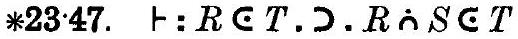
\includegraphics[max width=\textwidth, alt={}, center]{bc1848bf-39e8-4760-b069-9936044df683-088_39_518_300_209}\\
＊23．48． ト：$R$ C $S$ ． J．$R$ i $T$ C $S$ i $T$\\
＊23．481． ト：$R=S$ ．$\frac{\text { J．} R \text { ก } T=S \text { 五 } T}{}$\\
＊23．49．$\quad$ s：$P \in Q . R \in S$. J．$P \dot{\cap} R \in Q \dot{n} S$\\
＊2355．$\quad$ ．$R \dot{\circ} R=R$\\
＊2351． ト $R \dot{n} S=S \dot{n} R$\\
＊23．52．$\quad$ ．$(R \dot{n} S) \dot{n} T=R \dot{n}(S \dot{n} T)$\\
＊23．53．$R \dot{\cap} S \dot{\cap} T=(R \dot{\cap} S) \dot{n} T$ Df\\
＊23：54． 卜：$R=S$. J：$R$ C $T$ ．三．$S \subset T$\\
＊23：55．F：$R=S$. J：$T \in R . \equiv T \in S$\\
＊23．551． F $: R=S . \supset . R \mho T=S \cup T$\\
＊2356． ト．$R$ υ $R=R$\\
＊2357． ト．$R \mho S=S \cup R$\\
＊23：58．ト．$R$ C $R$ c $S$ ．$S \in R$ ʊ $S$\\
＊23．59． ト：$R$ C $T . S$ C $T . \equiv R$ © $S$ C $T$\\
＊23．6． ト：$x(R \cup S) y . \equiv: R \subset T . S \subset T . J_{T} . x T y$\\
＊23．61． । ：$R$ C $S$ ． J．$R$ C $S$ cT\\
＊23．62． $\mathrm{F}: R \in S . \equiv R \cup S=S$\\
＊23．621．$+: R \in S . \equiv . R \dot{n} S=R$\\
＊23．63．$\quad$ ．$R \mho(R \dot{\cap} S)=R$\\
＊23．631． ト．$R$ ก $(R \cup S)=R$\\
＊23．632．$+: R=S$. ɔ．$R=R$ í $S$\\
＊23．633．$\vdash: R$ ¢ $S$ ．J．$R$ υ $T=(R$ ก $S)$ 乞 $T$\\
＊23．64． ト：．$R$ C $T$ ．v．$S \subset T: \supset . R$ ก $S \subset T$\\
＊23．65． । ：$R$ C $S$ ．v．$R$ C $T$ ：J．$R$ C $S$ ण $T$\\
＊23．66． ト：$R$ C $S$ ． J．$R$ υ $T$ C $S$ υ $T$\\
＊23．68．$\quad$ ．$(R \dot{\hat{n}} S) \cup(R \dot{n} T)=R \dot{n}(S \cup T)$\\
＊23．69．$\quad \vdash .(R \mho S) \dot{\wedge}(R \mho T)=R \mho(S \dot{n} T)$\\
＊237．$\quad \vdash .(R \mho S) \mho T=R \mho(S \mho T)$\\
＊23．71．$R \mho S \mho T=(R \mho S) \mho T$ Df\\
＊2372． F ：$P \in R . Q \subset S . \supset . P \cup Q \subset R \cup S$\\
＊23．73．$F: P=R . Q=S . \supset . P \cup Q=R \mho S$\\
＊23．74．$\quad \mathrm{F}: P \dot{\cap} Q \subset R . P \dot{\cap} R \in Q . \equiv . P \dot{\cap} Q=P \dot{\cap} R$\\
＊238．$\quad$ ト．$-(-R)=R$\\
＊2381．F：$R$ CS．$\equiv$ ．$-S \subset-R$\\
＊23811．F：$R$ C－$S . \equiv . S \subset \doteq R$\\
＊2382． －$R$ i $S \subset T . \equiv R \cong T \mathbf{C} \in S$\\
＊2383． F $: R=S . \equiv .-R=-S$\\
＊23．831． t：$R=\dot{-} S . \equiv . S=\dot{-} R$\\
＊23．84． F．$\cdot(R \dot{\cap} S)=\dot{-} R \mho \dot{-} S$\\
＊2385．$\quad$ ．$R$ $\dot{\circ} S=\dot{-}(\dot{-} R \cup \dot{-} S)$\\
＊23．86． F．$-(\dot{-} R \dot{n}-S)=R \mho S$\\
＊2387．$\vdash .-R \dot{\circ}-S=-(R \mho S)$\\
＊23．88．ト．$(x, y) . x(R \cup \perp R) y$\\
＊23．89．ㅏ．$(x, y) . \sim\{x(R \doteq R) y\}$\\
＊23．9．$\quad$ ．$(R \cup S)-S=R-S$\\
＊23．91．ト．$R \mho S=R \mho(S \doteq R)$\\
＊23．92． F ：$R$ C $S$ ．ɔ ．$S=R$ υ $(S \doteq R)$\\
＊23．93．$+. R-S=R-(R \cap S)$\\
＊2394．$\vdash:(R) \cdot f R \cdot \equiv \cdot(R) \cdot f(-R)$\\
＊2395．$\vdash:(\mathrm{H} R) \cdot f R$ ．三．$(\mathrm{G} R) \cdot f(-R)$

\section*{*24. THE UNIVERSAL CLASS, THE NULL-CLASS, AND THE EXISTENCE OF CLASSES}
\section*{Summary of *24.}
The universal class, denoted by $V$, is the class of all objects of the type which, in the given context, is being denoted by small Latin letters, i.e. of the lowest type concerned. Thus V, like "Cls," is ambiguous as to type. Its definition is as follows:

\section*{*24:01. $\mathrm{V}=\hat{x}(x=x) \mathrm{Df}$}
Any other property possessed by everything would do as well as " $x=x$," but this is the only such property which we have hitherto studied.

The null-class, denoted by $\Lambda$, is the class which has no members. Like V , it is ambiguous as to type. We use the same symbol, $\Lambda$, for null-classes of various types; but these null-classes differ. The type of $\Lambda$ is determined by that of the terms $x$ concerning which " $x \in \Lambda$ " is false: whatever $x$ may be, " $x \in \Lambda$ " will not represent a true proposition, but unless $x$ is of the appropriate type, " $x \in \Lambda$ " will be meaningless, not false. Thus $\Lambda$ is of the type next above that of an $x$ concerning which " $x \in \Lambda$ " is significant and false. The definition of $\Lambda$ is

$$
\text { *24.02. } \quad \Lambda=-\mathrm{V} \text { Df }
$$

When a class $\alpha$ is not null, so that it has one or more members, it is said to exist. (This sense of " existence" must not be confused with that defined in *14.02.) We write " $4!\alpha$ " for " $\alpha$ exists." The definition is

\section*{*24.03. $A!\alpha .=.(H x) . x \in \alpha$ Df}
In the present number, we shall deal first with the properties of $\Lambda$ and $V$, then with those of existence. In comparing the algebra of symbolic logic with ordinary algebra, $\Lambda$ takes the place of 0 , while V combines the properties of 1 and of $\infty$.

Among the more important properties of $\Lambda$ and V which are proved in this number are the following:

\section*{*24-1. $\quad$. $\Lambda \neq \mathrm{V}$}
I.e. "nothing is not everything." This is useful as giving us the existence of at least two classes. If the monistic philosophers were right in maintaining that only one individual exists, there would be only two classes, $\Lambda$ and V , V being (in that case) the class whose only member is the one individual. Our primitive propositions do not require the existence of more than one individual.\\
＊24．102．103 show that any function which is always true determines the universal class，and any function which is always false determines the null－ class．\\
＊24．21．22 give forms of the laws of contradiction and excluded middle，namely ＂nothing is both $\alpha$ and not－$\alpha$＂（ $\alpha \cap-\alpha=\Lambda$ ）and＂everything is either $\alpha$ or not－$\alpha$＂（ $\alpha \cup-\alpha=\mathrm{V}$ ）．\\
＊24．23．24．26．27 give the properties of $\Lambda$ and V with respect to addition and multiplication，namely ：multiplication by V and addition of $\Lambda$ make no change in a class（ $* 24 \cdot 26 \cdot 24$ ）；addition of $V$ gives $V$ ，and multiplication by $\Lambda$ gives $\Lambda (* 24 \cdot 27 \cdot 23)$ ．It will be observed that the properties of $\Lambda$ and V result from each other by interchanging addition and multiplication．\\
＊243．$\quad \vdash: \alpha \subset \beta . \equiv \alpha-\beta=\Lambda$\\
I．e．＂$\alpha$ is contained in $\beta$＂is equivalent to＂nothing is $\alpha$ but not $\beta$ ．＂\\
＊24311．F：$\alpha \mathrm{C}-\beta . \equiv \alpha \cap \beta=\Lambda$\\
I．e．＂no $\alpha$ is a $\beta$＂is equivalent to＂nothing is both $\alpha$ and $\beta$ ．＂\\
＊24411．$+\beta$ ：$\beta$ C ． ɔ ．$\alpha=\beta \cup(\alpha-\beta)$\\
＊2443． ト ：$\alpha-\beta \cup_{\gamma . \equiv} \alpha \subset \beta \cup \gamma$\\
As a rule，propositions concerning $V$ are much less used than the corre－ lative propositions concerning $\Lambda$ ．

The properties of the existence of classes result from those of $\Lambda$ ，owing to the fact that $G!\alpha$ is the contradictory of $\alpha=\Lambda$ ，as is proved in $* 24.54$ ．Thus we have，in virtue of＊243，\\
＊24．55． $\mathrm{F}: \sim(\alpha \subset \beta) . \equiv$ ，子！$\alpha-\beta$\\
I．e．＂not all $\alpha$＇s are $\beta$＇s＂is equivalent to＂there are $\alpha$＇s which are not $\beta$＇s．＂ This is the familiar proposition of formal logic，that the contradictory of the universal affirmative is the particular negative．

We have\\
＊2456． F： 月！$(\alpha \cup \beta)$ ．$\equiv:$ 月！$\alpha$ ．v． 月！$\beta$\\
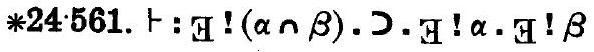
\includegraphics[max width=\textwidth, alt={}, center]{bc1848bf-39e8-4760-b069-9936044df683-091_52_594_1545_119}\\
I．e．if a sum exists，then one of the summands exists，and vice versa ；and if a product exists，both the factors exist（but not vice versa）．

The proofs of propositions in the present number offer no difficulty．

\begin{center}
\begin{tabular}{lll}
＊24．01． & $\mathrm{V}=\hat{x}(x=x)$ & Df \\
＊24．02． & $\Lambda=-\mathrm{V}$ & Df \\
＊24．03． & $\mathrm{H}!\alpha=-(\mathrm{H} x) . x \in \alpha$ & Df \\
＊24．1． & $\vdash . \Lambda \neq \mathrm{V}$ & $[* 22 \cdot 351 .(* 24 \cdot 02)]$ \\
＊24．101． $\mathrm{F} . \mathrm{V}=-\Lambda$ & $[* 22 \cdot 831 .(* 24 \cdot 02)]$ &  \\
\end{tabular}
\end{center}

＊24－102．$\vdash:(x) \cdot \phi x . \equiv . \hat{z}(\phi z)=\mathrm{V}$\\
Dem．

$$
\begin{array}{lrl}
\vdash \cdot * 13 \cdot 15 \cdot * 5 \cdot 501 . & \supset \vdash: \phi x \cdot \equiv: \phi x \cdot \equiv \cdot x=x: . \\
{[* 10 \cdot 11 \cdot 271]} & \supset \vdash: .(x) \cdot \phi x . & \equiv:(x): \phi x . \equiv . x=x: \\
& & \equiv: \hat{z}(\phi z)=\hat{z}(x=x): \\
{[* 20 \cdot 15]} & & \equiv: \hat{z}(\phi z)=\mathrm{V}: . \text { つf.Prop }
\end{array}
$$

Thus any function which is always true determines the universal class， and vice versa．\\
＊24＇103．$\vdash:(x) . \sim \phi x . \equiv . \hat{z}(\phi z)=\Lambda$\\
Dem．

$$
\begin{array}{ll}
\vdash \cdot * 24 \cdot 102 \cdot \supset \vdash:(x) \cdot \sim \phi x \cdot & \equiv: \hat{z}(\sim \phi z)=\mathrm{V}: \\
{[* 22 \cdot 392]} & \equiv:-\hat{z}(\phi z)=\mathrm{V}: \\
{[* 22 \cdot 831]} & \equiv: \hat{z}(\phi z)=-\mathrm{V}: \\
{[(* 24 \cdot 02)]} & \equiv: \hat{z}(\phi z)=\Lambda: . \supset \vdash . \text { Prop }
\end{array}
$$

＊24－104．$\vdash .(x) . x \in \mathrm{~V}$\\
Dem．


\begin{align*}
& \vdash \cdot * 20 \cdot 3 . \supset \vdash: x \in \mathrm{~V} . \equiv x=x  \tag{1}\\
& \vdash .(1) \cdot * 13 \cdot 15 . * 10 \cdot 11 \cdot 271 . \supset \vdash . \text { Prop }
\end{align*}


＊24－105．＋．$(x) . x \sim \epsilon$ Λ\\
Dem．


\begin{align*}
& \vdash \cdot * 22 \cdot 35 . \text { つ } \vdash: x \in \Lambda . \equiv . x \sim \epsilon \mathrm{~V}: \\
& {[* 4 \cdot 12] \quad \text { J }: x \sim \epsilon \Lambda . \equiv x \epsilon \mathrm{~V}}  \tag{1}\\
& \vdash .(1) \cdot * 10 \cdot 11 \cdot 271 . * 24 \cdot 104 . \text { つ } \text {. Prop }
\end{align*}


＊24－11．$\vdash .(\alpha) . \alpha \subset \mathrm{V}$\\
Dem．\\
ト．$* 24 \cdot 104 . * 10 \cdot 1$. つト．$x \in \mathrm{~V}$ ．

$$
\begin{array}{ll}
{[\operatorname{Simp}]} & \supset \vdash: x \in \alpha . \supset . x \in V: \\
{[* 10 \cdot 11 . * 22 \cdot 1]} & \supset \vdash: \alpha \subset V: \\
{[* 10 \cdot 11]} & \supset \vdash:(\alpha) \cdot \alpha \subset V: \supset \vdash . \text { Prop }
\end{array}
$$

＊24－12． ‥ $(\alpha) . \Lambda \subset \alpha$\\
Dem．

\[
\begin{array}{ll}
\vdash \cdot * 24 \cdot 105 \cdot * 10 \cdot 1 . & \supset \vdash \cdot x \sim \epsilon \Lambda . \\
{[* 2 \cdot 21]} & \supset \vdash: x \in \Lambda . \supset \cdot x \epsilon \alpha  \tag{1}\\
\vdash .(1) \cdot * 10 \cdot 11, * 22 \cdot 1 . \supset \vdash . \text { Prop }
\end{array}
\]

＊24．13．$\vdash: \alpha=\Lambda . \equiv \alpha \subset \Lambda$\\
Dem．

$$
\begin{aligned}
\vdash . * 24 \cdot 12 . * 4 \cdot 73 . \supset \vdash: \alpha \subset \Lambda . & \equiv . \alpha \subset \Lambda . \Lambda \subset \alpha . \\
& \equiv . \alpha=\Lambda: \supset \vdash . \text { Prop } \\
{[* 22 \cdot 41] } & =.
\end{aligned}
$$

＊24＇14．$\vdash:(x) . x \in \alpha . \equiv . \alpha=\mathrm{V}$\\
Dem．

$$
\begin{aligned}
\vdash \cdot * 24 \cdot 102 \cdot \supset \vdash:(x) \cdot x \in \alpha \cdot & \equiv \hat{x}(x \in \alpha)=\mathrm{V} . \\
& \equiv \cdot \alpha=\mathrm{V}: \supset \vdash . \text { Prop } \\
{[* 20 \cdot 32] } &
\end{aligned}
$$

＊24－141．＋： $\mathrm{VC} \alpha . \equiv . \mathrm{V}=\alpha$\\
Dem．

$$
\begin{aligned}
\vdash . * 24 \cdot 11 . * 4 \cdot 73 . \supset \vdash: \mathrm{VC} \alpha . & \equiv \alpha \subset \mathrm{V} . \mathrm{VC} \alpha . \\
{[* 22 \cdot 41] } & \equiv . \alpha=\mathrm{V}: \supset \vdash . \text { Prop }
\end{aligned}
$$

＊2415．$\vdash:(x) . x \sim \epsilon \alpha . \equiv . \alpha=\Lambda$\\
Dem．

$$
\begin{aligned}
\vdash \cdot * 24 \cdot 103 . \supset \vdash:(x) \cdot x \sim \epsilon \alpha . & \equiv . \hat{x}(x \in \alpha)=\Lambda . \\
{[* 20 \cdot 32] } & \equiv . \alpha=\Lambda: \supset \vdash . \text { Prop }
\end{aligned}
$$

＊24．17． $\mathrm{F}: \alpha=\mathrm{V} . \equiv .-\alpha=\Lambda[* 22.83 .(* 24.02)]$\\
＊24：21． ト．$\alpha \cap-\alpha=\Lambda \quad[* 24 \cdot 103 \cdot * 22 \cdot 89]$\\
＊24：22．ㅏ．$\alpha \cup-\alpha=\mathrm{V} \quad[* 22: 88 . * 24 \cdot 102]$\\
＊24：23． F．$\alpha \cap \mathrm{A}=\Lambda \quad$［＊24＇12．＊22．621］\\
＊24．24． ト．$\alpha \cup \Lambda=\alpha$［＊24．12．＊22．62］\\
The above two propositions（＊24－23－24）exhibit the algebraical analogy of $\Lambda$ to zero．\\
＊24：26．F．$\alpha \cap \mathrm{V}=\alpha \quad$［＊22．621．＊24．11］\\
This exhibits the analogy of V to 1 ．

\section*{＊24：27． ト．$\alpha \cup \mathrm{V}=\mathrm{V} \quad[* 22.62 . * 24.11]$}
This exhibits the analogy of V to $\infty$ ．\\
＊243．$\quad \vdash: \alpha \subset \beta . \equiv \alpha-\beta=\Lambda$\\
Dem．


\begin{align*}
& \text { F. } * 4 \cdot 53 \cdot 6 \cdot \nu \\
& \text { F: } x \in \alpha \cdot \nu \cdot x \in \beta: \equiv: \sim(x \in \alpha \cdot x \sim \epsilon \beta): \\
& {[* 22 \cdot 35] \quad \equiv: \sim(x \in \alpha \cdot x \epsilon-\beta):} \\
& {[* 22 \cdot 33] \quad \equiv: \sim(x \in \alpha-\beta)}  \tag{1}\\
& \text { F. }(1) \cdot * 10 \cdot 11 \cdot 271 . \nu \\
& \text { F: } \alpha \subset \beta \cdot \equiv .(x) \cdot \sim(x \in \alpha-\beta) . \\
& {[* 24 \cdot 15] \equiv \cdot \alpha-\beta=\Lambda: \nu \text {. Prop }}
\end{align*}


The above proposition is very frequently used．

\section*{＊2431． F ：$\alpha \subset \beta$ ．$\equiv$ ．$-\alpha \cup \beta=\mathrm{V}$}
Dem．

$$
\begin{array}{ll}
\vdash \cdot * 4 \cdot 6 . & \supset \vdash: x \in \alpha \cdot \supset \cdot x \in \beta: \equiv: x \sim \epsilon \alpha \cdot v \cdot x \in \beta: . \\
{[* 10 \cdot 11 \cdot 271] \supset \vdash:, \alpha \subset \beta .} & \equiv:(x): x \sim \epsilon \alpha \cdot v \cdot x \in \beta: \\
{[* 22 \cdot 35]} & \equiv:(x): x \epsilon-\alpha \cdot v \cdot x \in \beta: \\
{[* 22 \cdot 34]} & \equiv:(x) \cdot x \epsilon(-\alpha \cup \beta): \\
{[* 24 \cdot 14]} & \equiv:-\alpha \cup \beta=\mathrm{V}: . \supset \text {. Prop }
\end{array}
$$

This proposition is the correlative of $* 24 \cdot 3$ ，but，unlike that proposition， it is not useful in the sequel．Every proposition concerning $\Lambda$ has a corre－ lative concerning V，but we shall often not give these correlatives，since they are seldom required for subsequent proofs．\\
＊24：311． $\mathrm{F}: \alpha \mathrm{C}-\beta . \equiv \alpha \cap \beta=\Lambda$\\
Dem．


\begin{align*}
& \text { ト. *2235. } \text { つ } \text { : } x \in \alpha \text {. } \text { J. } x \epsilon-\beta: \equiv: x \epsilon \alpha \text {. } \text { J. } x \sim \epsilon \beta \text { : } \\
& \text { [*4:51.62] } \equiv: \sim(x \in \alpha . x \in \beta) \text { : } \\
& \text { [*22:33] } \quad \equiv: \sim(x \in \alpha \cap \beta)  \tag{1}\\
& \text { ㅏ.(1). } * 10 \cdot 11 \cdot 271 . \text { つ }: \alpha C-\beta . \equiv(x) \cdot x \sim \epsilon \alpha \sim \beta \text {. } \\
& \text { [*24•15] } \quad \equiv \text {. } \alpha \cap \beta=\Lambda: \supset \vdash \text {. Prop }
\end{align*}


＊24312． $\mathrm{F}:-\alpha \mathrm{C} \beta . \equiv . \alpha \cup \beta=\mathrm{V}$\\
Dem．

$$
\begin{array}{lrl}
\vdash . * 2235 . \supset \vdash: .-\alpha \subset \beta . & \equiv: x \sim \epsilon \alpha . \partial_{x} . x \in \beta: \\
{[* 4: 64]} & \equiv:(x): x \in \alpha . \vee . x \in \beta: \\
{[* 22: 34]} & \equiv:(x) . x \in \alpha \cup \beta: \\
{[* 24 \cdot 14]} & \equiv: \alpha \cup \beta=\mathrm{V}: . \supset F . \text { Prop }
\end{array}
$$

＊24：313． $\mathrm{F}: \alpha \cap \beta=\Lambda . \equiv \alpha=\alpha-\beta$［＊24：311．＊22．621］\\
＊2432．F：$\alpha \cup \beta=\Lambda . \equiv \alpha=\Lambda . \beta=\Lambda$\\
Dem．

$$
\begin{aligned}
\vdash \cdot * 24 \cdot 13 . \text { つf: } \alpha \cup \beta=\Lambda . & \equiv: \alpha \cup \beta \subset \Lambda: \\
{[* 22 \cdot 59] } & \equiv: \alpha \subset \Lambda . \beta \subset \Lambda: \\
{[* 24 \cdot 13] } & \equiv: \alpha=\Lambda . \beta=\Lambda: . \supset \vdash . \text { Prop }
\end{aligned}
$$

＊2433．$\vdash: \alpha=V . \supset . \alpha \cup \beta=V$\\
Dem．

$$
\begin{aligned}
\vdash \cdot * 22 \cdot 551 . \supset \vdash: \mathrm{Hp} . \supset . \alpha \cup \beta & =\mathrm{V} \cup \beta \\
{[* 24 \cdot 27 \cdot * 22 \cdot 57] } & =\mathrm{V}: \supset \vdash . \text { Prop }
\end{aligned}
$$

＊24．34． F：$\alpha=\Lambda$. J．$\alpha \cap \beta=\Lambda$［ $* 22.481 . * 24.23$ ］\\
＊2435． $\mathrm{F}: \alpha=\mathrm{V}$. つ．$\alpha \cap \beta=\beta \quad[* 22.481 . * 24.26]$\\
＊24：36． $\mathrm{F}: \alpha=\Lambda$. つ．$\alpha \cup \beta=\beta$［＊22：551．＊24＊24］\\
＊24：37． F：$\alpha \cap \beta=\Lambda . \equiv: x \in \alpha . y \in \beta . \supset_{x, y} . x \neq y$\\
Dem．

$$
\begin{array}{lrl}
\vdash . * 24 \cdot 15 . & \text { JF: } \alpha \cap \beta=\Lambda . & \equiv:(x) . x \sim \epsilon(\alpha \cap \beta): \\
& \equiv:(x) . \sim(x \in \alpha . x \in \beta): \\
{[* 22 \cdot 33]} & \equiv:(x, y): x=y . \supset . \sim(x \in \alpha . y \epsilon \beta): \\
{[* 13 \cdot 191]} & \equiv:(x, y): x \in \alpha . y \in \beta . \supset . x \neq y: . \supset F . \text { Prop } \\
\text { [Transp] } &
\end{array}
$$

＊24：38． $\mathrm{F}: \alpha \sim \beta=\Lambda . \mathrm{D}: \alpha \neq \beta . \mathrm{v} . \alpha=\Lambda . \beta=\Lambda$\\
Dem．\\
ト．$* 22 \cdot 481$. つト：$\alpha \cap \beta=\Lambda . \alpha=\beta$ ．J．$\alpha \cap \alpha=\Lambda$ ．

\[
\begin{array}{ll}
{[* 22 \cdot 5]} & \supset \cdot \alpha=\Lambda \cdot \\
{[* 20 \cdot 23]} & \supset \cdot \alpha=\Lambda \cdot \beta=\Lambda \\
\vdash \cdot(1) \cdot \operatorname{Exp} \cdot \supset \vdash: \cdot \alpha \cap \beta=\Lambda \cdot \supset: & \alpha=\beta \cdot \supset \cdot \alpha=\Lambda \cdot \beta=\Lambda:  \tag{1}\\
{[* 4 \cdot 6]} & \supset: \alpha \neq \beta \cdot v \cdot \alpha=\Lambda \cdot \beta=\Lambda: \supset F . \text { Prop }
\end{array}
\]

＊2439． F：$\alpha \cap \beta=\Lambda . \equiv: x \in \alpha . \partial_{x} . x \sim \epsilon \beta$［＊24311．＊2235］\\
＊244．$\quad \vdash: \alpha \cap \beta=\Lambda . \equiv .(\alpha \cup \beta)-\alpha=\beta . \equiv .(\alpha \cup \beta)-\beta=\alpha$\\
Dem．


\begin{align*}
& \text { ト. } * 24311 . \text { つト }: \alpha \cap \beta=\Lambda . \equiv \beta \mathrm{C}-\alpha . \\
& \text { [*22.621] } \quad \equiv . \beta-\alpha=\beta \text {. } \\
& {[* 22.9] \quad \equiv .(\alpha \cup \beta)-\alpha=\beta}  \tag{1}\\
& \text { f. (1) } \frac{\beta, \alpha}{\alpha, \beta} \text {. } \supset \vdash: \beta \cap \alpha=\Lambda . \equiv:(\beta \cup \alpha)-\beta=\alpha \text { : } \\
& {[* 22 \cdot 51 \cdot 57] \text { ว! } \alpha \cap \beta=\Lambda . \equiv(\alpha \cup \beta)-\beta=\alpha}  \tag{2}\\
& \text { ト.(1).(2). ɔㄴ. Prop }
\end{align*}


＊24401．$\vdash: \beta \subset \alpha$. ɔ $.(\beta \cup \gamma)-\alpha=\gamma-\alpha$\\
Dem．


\begin{align*}
& \vdash \cdot * 22 \cdot 68 . \supset \vdash \cdot(\beta \cup \gamma)-\alpha=(\beta-\alpha) \cup(\gamma-\alpha)  \tag{1}\\
& \vdash \cdot * 24 \cdot 3 . \supset \vdash: \mathrm{Hp} . \supset \cdot \beta-\alpha=\Lambda  \tag{2}\\
& \vdash .(1) \cdot(2) . \supset \vdash: \mathrm{Hp} . \supset .(\beta \cup \gamma)-\alpha=\Lambda \cup(\gamma-\alpha) \\
& {[* 24 \cdot 24]} \\
& =\gamma-\alpha: \supset \text {. Prop }
\end{align*}


＊24：402． $\mathrm{F}: \alpha \cap \beta=\Lambda . \xi \mathrm{C} \alpha . \eta \mathrm{C} \beta$. J．$\xi \cap \eta=\Lambda$\\
Dem．

$$
\begin{array}{ll}
\text { ト. } * 22 \cdot 49 . \text { つl: Hp. } & \text { J. } \xi \cap \eta \text { Can } \beta . \\
{[* 22 \cdot 55]} & \text { J. } \xi \cap \eta \subset \Lambda . \\
{[* 24 \cdot 13]} & \text { J. } \xi \cap \eta=\Lambda: \supset \vdash . \text { Prop }
\end{array}
$$

＊2441．F．$\alpha=(\alpha \cap \beta) \cup(\alpha-\beta)$\\
Dem．

$$
\begin{aligned}
\vdash . * 22.68 . \supset \vdash .(\alpha \cap \beta) \cup(\alpha-\beta) & =\alpha \cap(\beta \cup-\beta) \\
& =\alpha \cap \mathrm{V} \\
{[* 24 \cdot 22] } & =\alpha . \supset \vdash . \text { Prop } \\
{[* 24 \cdot 26] } & =
\end{aligned}
$$

＊24411． $\mathrm{F}: \beta$ C $\alpha$. J．$\alpha=\beta \cup(\alpha-\beta)$\\
Dem．

$$
\begin{aligned}
\vdash \cdot * 22 \cdot 633 \frac{\beta, \alpha, \alpha-\beta}{\alpha, \beta, \gamma} \cdot \supset \vdash: \beta \subset \alpha \cdot \supset \cdot \beta \cup(\alpha-\beta) & =(\alpha \cap \beta) \cup(\alpha-\beta) \\
& =\alpha: \supset F . \text { Prop }
\end{aligned}
$$

＊24：412． t $: \beta$ C $\alpha . \gamma$ C $\beta$. ɔ $.(\alpha-\beta) \cup(\beta-\gamma)=\alpha-\gamma$\\
Dem．

$$
\begin{aligned}
& \vdash \cdot * 24 \cdot 41 . \supset \vdash: \mathrm{Hp} . \supset .(\alpha-\beta) \cup(\beta-\gamma)=(\alpha-\beta \cap \gamma) \cup(\alpha-\beta-\gamma) \cup(\beta-\gamma) \\
& {[* 24 \cdot 3 \cdot 23]} \\
& {[* 22 \cdot 68]} \\
& {[* 24 \cdot 411]} \\
& =\{(\alpha-\beta) \cup \beta\}-\gamma \\
& =\{(\alpha-\gamma) \cup(\beta-\gamma) \\
& =\alpha-\gamma: \supset \vdash . \text { Prop }
\end{aligned}
$$

This proposition is used in $* 234 \cdot 181$ ，in the theory of continuous functions．\\
＊2442． $\mathrm{F}: \alpha \cap_{\beta} \mathrm{C}_{\gamma . \alpha}-\beta \mathrm{C}_{\gamma .} \equiv \alpha \mathrm{C}_{\gamma}$\\
Dem．

$$
\begin{aligned}
\vdash . * 22 \cdot 59 . \supset \vdash: \alpha \cap \beta \cup_{\gamma . \alpha-\beta} C_{\gamma} & \equiv(\alpha \cap \beta) \cup(\alpha-\beta) C_{\gamma .} \\
& \equiv . \alpha C_{\gamma}: \supset \vdash . \text { Prop } \\
{[* 24 \cdot 41] } &
\end{aligned}
$$

＊2443．$\vdash: \alpha-\beta C_{\gamma . \equiv . \alpha} \subset \beta \cup \gamma$\\
Dem．


\begin{align*}
& \text { ト. } * 56 \text {. } \supset+:: x \in \alpha . x \sim \epsilon \beta . \supset . x \in \gamma: \equiv: x \in \alpha . \supset: x \in \beta . \text { v. } x \in \gamma: . \\
& {[* 223533] \supset \vdash:: x \in \alpha-\beta . \supset . x \in \gamma: \equiv: x \in \alpha . \supset: x \in \beta . \mathbf{v} . x \in \gamma: .} \\
& {[* 2234] \quad \equiv: x \in \alpha . \supset . x \in(\beta \cup \gamma)}  \tag{1}\\
& \text { ト.(1). } * 10 \cdot 11 \cdot 271 . \text { つト. Prop }
\end{align*}


＊24431．$+.(\alpha \cup \gamma) \cap(\beta \cup-\gamma)=(\alpha \cap \beta) \cup(\alpha-\gamma) \cup(\beta \cap \gamma)$\\
This and the following proposition are lemmas for $* 24 \cdot 44$ ．\\
Dem．

$$
\begin{array}{ll}
\vdash . * 22.68 . \supset \vdash .(\alpha \cup \gamma) \cap(\beta \cup-\gamma) & =\{(\alpha \cup \gamma) \cap \beta\} \cup\{(\alpha \cup \gamma) \cap-\gamma\} \\
{[* 22.68]} & =(\alpha \cap \beta) \cup(\gamma \cap \beta) \cup(\alpha-\gamma) \cup(\gamma-\gamma) \\
{[* 24.21]} & =(\alpha \cap \beta) \cup(\gamma \cap \beta) \cup(\alpha-\gamma) \cup \Lambda \\
{[* 24 \cdot 24]} & =(\alpha \cap \beta) \cup(\gamma \cap \beta) \cup(\alpha-\gamma) \\
{[* 22.51 \cdot 57]} & =(\alpha \cap \beta) \cup(\alpha-\gamma) \cup(\beta \cap \gamma) . \supset \vdash . \text { Prop }
\end{array}
$$

＊24．432．$.(\alpha-\gamma) \cup(\beta \cap \gamma)=(\alpha \cap \beta) \cup(\alpha-\gamma) \cup(\beta \cap \gamma)$

\section*{Dem．}
$$
\begin{aligned}
& \text { ト. } * 24 \cdot 22 \cdot 35 \text {. } \text { ɔ } . \alpha \cap \beta=(\alpha \cap \beta) \cap(\gamma \cup-\gamma) \\
& \text { [*22.68] } \quad=(\alpha \cap \beta \cap \gamma) \cup(\alpha \cap \beta-\gamma) \\
& {[* 22 \cdot 51] \quad=(\alpha \cap \beta \cap \gamma) \cup(\alpha \cap-\gamma \cap \beta) .} \\
& {[* 22.551] \quad \supset \vdash .(\alpha \cap \beta) \cup(\alpha-\gamma)=(\alpha \cap \beta \cap \gamma) \cup(\alpha \cap-\gamma \cap \beta) \cup(\alpha-\gamma)} \\
& \text { [*22.63] }=(\alpha \cap \beta \cap \gamma) \cup(\alpha-\gamma) \\
& {[* 22.57] \quad=(\alpha-\gamma) \cup(\alpha \cap \beta \cap \gamma) .} \\
& {[* 22.551] \quad \supset \vdash .(\alpha \cap \beta) \cup(\alpha-\gamma) \cup(\beta \cap \gamma)=(\alpha-\gamma) \cup(\alpha \cap \beta \cap \gamma) \cup(\beta \cap \gamma)} \\
& \text { [*22.63] = }(\alpha-\gamma) \cup(\beta \cap \gamma) \text {. } \text { ɔ } \text {. Prop }
\end{aligned}
$$

＊2444．$\quad$ ．$(\alpha \cup \gamma) \cap(\beta \cup-\gamma)=(\alpha \cap-\gamma) \cup(\beta \cap \gamma) \quad$［＊24．431．432］\\
＊2445．$\vdash:(\alpha \cap \gamma) \cup(\beta-\gamma)=\Lambda . \equiv \beta \subset \gamma . \gamma \subset-\alpha$\\
Dem．

$$
\begin{aligned}
\vdash \cdot * 24 \cdot 32 \cdot \supset \vdash:(\alpha \cap \gamma) \cup(\beta-\gamma)=\Lambda & \equiv \cdot \alpha \cap \gamma=\Lambda \cdot \beta-\gamma=\Lambda . \\
& \equiv \cdot \gamma \subset-\alpha \cdot \beta \subset \gamma: \supset \vdash . \text { Prop } \\
{[* 24 \cdot 3 \cdot 311] } & =.
\end{aligned}
$$

＊2446．$\vdash:(\alpha \cap \gamma) \cup(\beta-\gamma)=\Lambda$. J．$\alpha \cap \beta=\Lambda$\\
Dem．

$$
\begin{array}{ll}
\vdash \cdot * 24 \cdot 45 \cdot * 22 \cdot 44 \cdot \supset \vdash: \mathrm{Hp} \cdot & \supset \cdot \beta \subset-\alpha \cdot \\
{[* 22 \cdot 811]} & \supset \cdot \alpha C-\beta \\
{[* 24 \cdot 311]} & \supset \cdot \alpha \cap \beta=\Lambda: \supset \vdash . \text { Prop }
\end{array}
$$

The following propositions，down to $* 24 \cdot 495$ inclusive，are lemmas inserted for use in much later propositions，most of them being only used a few times．\\
＊2447．$\vdash: \alpha \cap \beta=\Lambda . \alpha \cup \beta=\gamma . \equiv . \alpha C_{\gamma . \beta}=\gamma-\alpha$\\
Dem．\\
ト．$* 24311$. つト $: \alpha \cap \beta=A . \equiv \beta \subset-\alpha$

ト．＊2241． J ：$\alpha \cup \beta=\gamma . \equiv \alpha \cup \beta \subset \gamma . \gamma \subset \alpha \cup \beta$ ．\\
［ $* 22.59 . * 24.43$ ］

$$
\equiv . \alpha \mathbf{C}_{\gamma \cdot \beta} \mathbf{C}_{\gamma \cdot \gamma-\alpha} \mathbf{C} \beta
$$

$\vdash \cdot(1) \cdot(2) \cdot \supset \vdash: \alpha \cap \beta=\Lambda \cdot \alpha \cup \beta=\gamma \cdot \equiv \cdot \beta \subset-\alpha \cdot \alpha C_{\gamma \cdot \beta} C_{\gamma \cdot \gamma-\alpha} \subset \beta$ ．\\
［＊4：3］\\
$\equiv . \alpha \mathrm{C}_{\gamma \cdot \beta} \mathrm{C}_{\gamma \cdot \beta} \mathrm{C}-\alpha \cdot \gamma-\alpha \mathrm{C} \beta$.\\
［＊22•45］\\
$\equiv . \alpha \mathrm{C}_{\gamma \cdot \beta} \mathrm{C}_{\gamma-\alpha \cdot \gamma-\alpha} \mathrm{C} \beta$.\\
［＊22•41］\\
$\equiv . \alpha \mathrm{C}_{\gamma} . \beta=\gamma-\alpha:$ つ ㄱ．Prop\\
＊24．48．$\vdash: . \xi \subset \alpha . \xi^{\prime} \subset \alpha . \eta \subset \beta . \eta^{\prime} \subset \beta . \alpha \cap \beta=\Lambda . \supset$ ：


\begin{equation*}
\xi \cup \eta=\xi^{\prime} \cup \eta^{\prime} \cdot \equiv \cdot \xi=\xi^{\prime} \cdot \eta=\eta^{\prime} \tag{1}
\end{equation*}


Dem．\\
ト．$* 22 \cdot 73$ ．$\quad \supset \vdash: \xi=\xi^{\prime} \cdot \eta=\eta^{\prime} \cdot \supset \cdot \xi \cup \eta=\xi^{\prime} \cup \eta^{\prime}$

ト ．＊22．481．$\supset \vdash: . \xi \cup \eta=\xi^{\prime} \cup \eta^{\prime} . \supset:(\xi \cup \eta) \cap \alpha=\left(\xi^{\prime} \cup \eta^{\prime}\right) \cap \alpha:$\\
［＊22．68］ כ：$(\xi \cap \alpha) \cup(\eta \cap \alpha)=\left(\xi^{\prime} \cap \alpha\right) \cup\left(\eta^{\prime} \cap \alpha\right)$

ト．＊22．621．$\quad$ J ：$\xi \subset \alpha$. J．$\xi \cap \alpha=\xi: \xi^{\prime} \subset \alpha$. つ．$\xi^{\prime} \cap \alpha=\xi^{\prime}$ ：\\
［＊3＊47］$\supset \vdash: \xi \subset \alpha . \xi^{\prime} \subset \alpha . \supset . \xi \cap \alpha=\xi . \xi^{\prime} \cap \alpha=\xi^{\prime}$

ト．＊22．48．ɔト：$\eta \subset \beta . \supset . \eta \cap \alpha \subset \alpha \cap \beta$ ：\\
［＊22：55］\\
$\supset \vdash: \eta \subset \beta . \alpha \cap \beta=\Lambda . \supset . \eta \cap \alpha \subset \Lambda$.\\
［ $* 24 \cdot 13$ ］


\begin{equation*}
\text { כ. } \eta \cap \alpha=\Lambda \tag{4}
\end{equation*}


Similarly $\quad \vdash: \eta^{\prime} \subset \beta . \alpha \cap \beta=\Lambda . \supset . \eta^{\prime} \cap \alpha=\Lambda$

ㅏ．（3）．（4）．ɔํ：．Hp．$\supset:(\xi \cap \alpha) \cup(\eta \cap \alpha)=\xi \cup \Lambda$\\
［＊24＇24］

$$
=\xi
$$

ㅏ．（3）．（5）．ɔㅡ：．Hp．ɔ：$\left(\xi^{\prime} \cap \alpha\right) \cup\left(\eta^{\prime} \cap \alpha\right)=\xi^{\prime} \cup \Lambda$\\
［＊24：24］

ト．（2）．（6）．（7）．$\supset \vdash: \mathrm{Hp} \cdot \supset: \xi \cup \eta=\xi^{\prime} \cup \eta^{\prime} \cdot \supset \cdot \xi=\xi^{\prime}$

Similarly

$$
\vdash: \text { : Нр } . \supset: \xi \cup \eta=\xi^{\prime} \cup \eta^{\prime} . \supset . \eta=\eta^{\prime}
$$

ト．（1）．（8）．（9）．ɔ ⊢ ．Prop\\
The above proposition，besides being used in the next two，is used in the theory of couples（＊54．6），in the theory of greater and less（＊117．632），and in the chapter on the ordering of classes by the principle of first differences （ $* 170.68$ ）．\\
＊24：481．$\vdash: \alpha \cap \beta=\Lambda . \alpha \cap \gamma=\Lambda . \supset: \alpha \cup \beta=\alpha \cup \gamma . \equiv . \beta=\gamma$\\
Dem．\\
$\vdash \cdot * 24 \cdot 48 \frac{\alpha,-\alpha, \alpha \cdot \alpha, \beta, \gamma}{\alpha, \beta, \xi, \xi^{\prime}, \eta, \eta^{\prime}} \cdot \supset$\\
t：$\alpha$ C $\alpha \cdot \alpha$ C $\alpha \cdot \beta$ C $-\alpha \cdot \gamma$ C $-\alpha \cdot \alpha-\alpha=$ A． J：


\begin{equation*}
\alpha \cup \beta=\alpha \cup \gamma \cdot \equiv \cdot \alpha=\alpha \cdot \beta=\gamma \tag{1}
\end{equation*}


ト．$* 2242 . * 2421.3$

F ：$\alpha$ C $\alpha \cdot \alpha$ C $\alpha \cdot \beta$ C $-\alpha \cdot \gamma$ C $-\alpha \cdot \alpha-\alpha=\Lambda . \equiv, \beta$ C $-\alpha \cdot \gamma$ C $-\alpha$ ．


\begin{equation*}
[* 24311] \quad \equiv . \alpha \cap \beta=\Lambda . \alpha \cap \gamma=\Lambda \tag{2}
\end{equation*}


ト．$* 20 \cdot 2 \cdot * 4 \cdot 73$. J $: \alpha=\alpha \cdot \beta=\gamma \cdot \equiv \cdot \beta=\gamma$

ト．（1）．（2）．（3）．ɔㄴ．Prop\\
The above proposition is used in the theory of selections（＊83．74），in the theory of greater and less（＊117582），and in the theory of transfinite induction （＊257）．\\
＊24：482． $\mathrm{F}: . \xi \mathrm{C} \alpha . \eta \mathrm{C} \beta . \alpha \cap \beta=\mathrm{A} . \supset: \xi \cup \eta=\alpha \cup \beta . \equiv . \xi=\alpha . \eta=\beta$

$$
\left[* 24 \cdot 48 \frac{\alpha, \beta}{\xi^{\prime}, \eta^{\prime}} * 22 \cdot 42\right]
$$

The above proposition is used in the theory of convergence（＊23234）．\\
＊24．49． F：$\alpha \cap \beta=\Lambda . \supset: \alpha \subset \beta \cup_{\gamma .} \equiv \alpha \subset_{\gamma}$\\
Dem．


\begin{align*}
& \text { ト. } * 22621 . \supset \vdash: \alpha \subset \beta \cup \gamma . \equiv \alpha=\alpha \cap(\beta \cup \gamma) \\
& {[* 22.68] \quad=(\alpha \cap \beta) \cup(\alpha \cap \gamma)}  \tag{1}\\
& \text { ト. *24.24. ɔト: } \alpha \cap \beta=\Lambda . \supset .(\alpha \cap \beta) \cup(\alpha \cap \gamma)=\alpha \cap \gamma  \tag{2}\\
& \text { ト.(1).(2). ɔ :. Hp. ɔ: } \alpha \subset \beta \cup \gamma . \equiv \alpha=\alpha \cap \gamma \text {. } \\
& \text { [*22.621] } \\
& \equiv . \alpha \text { C }_{\gamma} \text { : ɔ . Prop }
\end{align*}


＊24491．$f: \beta \cap \gamma=\Lambda . \alpha \subset \beta \cup \gamma$.

$$
\nu \cdot \alpha-\beta=\alpha \cap \gamma \cdot \alpha-\gamma=\alpha \cap \beta \cdot \alpha=(\alpha-\beta) \cup(\alpha-\gamma)
$$

Dem．

\[
\begin{array}{lc}
\vdash \cdot * 22 \cdot 621 . & \supset \vdash: \mathrm{Hp} . \supset . \alpha=\alpha \cap(\beta \cup \gamma) . \\
{[* 22 \cdot 481]} & \supset . \alpha-\gamma=\alpha \cap(\beta \cup \gamma)-\gamma \\
{[* 24 \cdot 4]} & =\alpha \cap \beta \\
\text { Similarly } & \vdash: \mathrm{Hp} . \supset . \alpha-\beta=\alpha \cap \gamma  \tag{2}\\
\begin{array}{l}
\vdash .(1) .(2) . \\
{[* 22.68]}
\end{array} & \supset \vdash: \mathrm{Hp} . \supset .(\alpha-\beta) \cup(\alpha-\gamma) \\
{[* 22.621]} & \\
& =\alpha \cap \gamma) \cup(\alpha \cap \beta) \\
& =\alpha \cap(\gamma \cup \beta) \\
& =\alpha
\end{array}
\]

ト．（1）．（2）．（3）．ɔ ⊢ ．Prop\\
The above proposition is used in the theory of selections（＊83．63．65）and in the theory of segments of a series（ $* 211 \cdot 84$ ）．\\
＊24．492． ㅏ：$\beta$ C $\alpha \cdot \alpha-\beta=\gamma \cdot$ ɔ $\alpha-\gamma=\beta$\\
Dem．

$$
\begin{array}{ll}
\vdash \cdot * 22 \cdot 481 . \supset \vdash: \mathrm{Hp} . \supset . \alpha-\gamma & =\alpha-(\alpha-\beta) \\
{[* 22 \cdot 8 \cdot 86]} & =\alpha \cap(-\alpha \cup \beta) \\
{[* 22 \cdot 8 \cdot 9]} & =\alpha \cap \beta \\
{[* 22 \cdot 621]} & =\beta: \supset \vdash . \text { Prop }
\end{array}
$$

The above proposition is used fairly frequently，especially in the theory of series．It is first used in $* 93 \cdot 273$ ，in the theory of＂generations．＂\\
＊24．493．$+: \beta \cap \gamma=\Lambda$. つ $. \alpha=(\alpha-\beta) \cup(\alpha-\gamma)$\\
Dem．

$$
\begin{aligned}
& \vdash \cdot * 22 \cdot 84 \cdot * 24 \cdot 17 \cdot \supset \vdash: \mathrm{Hp} \cdot \supset \cdot-\beta \cup-\gamma=\mathrm{V} \\
& \begin{array}{lr}
{[* 24 \cdot 26]} & \supset \cdot \alpha=\alpha \cap(-\beta \cup-\gamma) \\
{[* 22 \cdot 68]} & =(\alpha-\beta) \cup(\alpha-\gamma): \supset \vdash . \text { Prop }
\end{array}
\end{aligned}
$$

＊24．494． F：$\xi$ C $\alpha . \eta$ C $\beta . \alpha \cap \beta=\Lambda$. つ．$(\xi \cup \eta)-\alpha=\eta .(\xi \cup \eta)-\beta=\xi$\\
Dem．

\[
\begin{array}{lc}
\vdash \cdot * 24 \cdot 3 . & \supset \vdash: \mathrm{Hp} \cdot \supset \cdot \xi-\alpha=\Lambda \\
\vdash \cdot * 24 \cdot 311 . & \supset \vdash: \mathrm{Hp} \cdot \supset \cdot \beta \subset-\alpha . \\
{[* 22 \cdot 44]} & \supset \cdot \eta \subset-\alpha . \\
{[* 22 \cdot 621]} & \supset \cdot \eta-\alpha=\eta \\
\vdash \cdot * 22 \cdot 68 . & \supset \vdash \cdot(\xi \cup \eta)-\alpha=(\xi-\alpha) \cup(\eta-\alpha) \\
\vdash \cdot(1) \cdot(2) \cdot(3) \cdot * 24 \cdot 24 . \supset \vdash: \mathrm{Hp} \cdot \supset \cdot(\xi \cup \eta)-\alpha=\eta \\
\text { Similarly } & \vdash: \mathrm{Hp} \cdot \supset \cdot(\xi \cup \eta)-\beta=\xi  \tag{5}\\
\vdash \cdot(4) \cdot(5) . & \supset \vdash . \text { Prop }
\end{array}
\]

This proposition is used in the theory of selections（ $* 83.63$ and $* 88.45$ ）．\\
＊24．495． $\mathrm{F}: \alpha \cap \gamma=\Lambda$. J．$(\alpha \cup \gamma)-(\beta \cup \gamma)=\alpha-\beta$\\
Dem．


\begin{align*}
& \vdash \cdot * 22 \cdot 87 \cdot 68 \cdot \supset \\
& \vdash \cdot(\alpha \cup \gamma)-(\beta \cup \gamma)=(\alpha-\beta-\gamma) \cup(\gamma-\beta-\gamma) \\
& {[* 24 \cdot 21] \quad=\alpha-\beta-\gamma}  \tag{1}\\
& \vdash \cdot * 24 \cdot 311 \cdot * 22 \cdot 621 \cdot \supset \vdash: \mathrm{Hp} \cdot \supset \cdot \alpha-\gamma=\alpha  \tag{2}\\
& \vdash \cdot(1) \cdot(2) \cdot \quad \supset \vdash \cdot \text { Prop }
\end{align*}


The above proposition is used in the theory of minimum points （ $* 205 \cdot 83 \cdot 832 \cdot 84$ ）．

In the remainder of this number we shall be concerned with the existence of classes．Many of the properties of the existence of classes follow from the fact that to say a class exists is equivalent to saying that the class is not equal to the null－class．This is proved in $* 2454$ ．\\
＊245．$\vdash: \mathcal{H}!\alpha . \equiv .\left(H^{x}\right) . x \in \alpha \quad[* 4 \cdot 2 .(* 2403)]$\\
＊2451．$\vdash: \sim A!\alpha . \equiv . \alpha=\Lambda$\\
Dem．

$$
\begin{aligned}
\vdash . * 245 . \supset \vdash: \sim G!\alpha . & \equiv \sim \sim(\mathrm{H} x) . x \in \alpha\} . \\
{[* 10.252] } & \equiv .(x) . x \sim \epsilon \alpha . \\
{[* 24 \cdot 15] } & \equiv . \alpha=\Lambda: \supset \vdash . \text { Prop }
\end{aligned}
$$

＊24：52． ト．A！V［＊24：51•1．Transp］\\
This proposition states that the class of all objects of the type in question is not null，but has at least one member．The assumption that there is some－\\
thing，which is equivalent to this proposition，is implicit in the proposition ＊10．1，that what is true always is true in any instance．This would not hold if there were no instances of anything；hence it implies the existence of something．It will be observed that the above proposition（＊24．52）depends on $* 24 \cdot 1$ ，which depends on $* 22 \cdot 351$ ，which depends on $* 10 \cdot 251$ ，which depends on $* 10 \cdot 24$ ，which depends on $* 10 \cdot 1$ or on $* 9 \cdot 1$ ．The assumption that there is something is involved in the use of the real variable，which would otherwise be meaningless．This is made explicit in $* 9 \cdot 1$ ，and in the proof of $* 9 \cdot 2$ ，which is the same proposition as $* 10 \cdot 1$ ．\\
＊24：53．ト．～马！$\Lambda$\\
＊24．54． ト： $\mathbb{G}$ ！$\alpha . \equiv \alpha \neq \Lambda$\\
＊24：55． F：$\sim(\alpha \subset \beta) . \equiv . H!\alpha-\beta$\\
＊24：56． ト：$H$ ！$(\alpha \cup \beta)$ ．$\equiv: \mathcal{H}!\alpha$ ．v．$H!\beta$\\
＊24：561． ト： 月！$(\alpha \cap \beta)$ ． J． 月！$\alpha$ ． T！$\beta$\\
$[* 24 \cdot 51 \cdot * 20 \cdot 2]$\\
［＊24：51．Transp］\\
［＊24：3．Transp．＊24：54］\\
［＊10．42．＊22：34］\\
［＊10．5．＊22．33］\\
＊24：57， 卜：$\alpha \cap \beta=\Lambda . \supset: \mathcal{H}$ ！$\alpha . \supset . \alpha \neq \beta$\\
Dem．

$$
\begin{array}{ll}
\vdash \cdot * 22 \cdot 481 . \supset \vdash: \alpha \cap \beta=\Lambda . \alpha=\beta . & \text { J. } \alpha \cap \alpha=\Lambda . \\
{[* 22 \cdot 5]} & \text { J. } \alpha=\Lambda . \\
{[* 24 \cdot 51]} & \text { J. } \sim H!\alpha \\
\vdash .(1) \cdot \text { Exp. Transp. } \supset \vdash . \text { Prop } &
\end{array}
$$

＊24：571． ト： Д ！$\alpha$ ．$\alpha=\beta$ ．Э． Д！$(\alpha \cap \beta)$\\
Dem．\\
ト．$* 24 * 57 . \mathrm{Comm} . \supset \vdash:$ ： $\mathrm{H}!\alpha . \supset: \alpha \cap \beta=\Lambda . \supset . \alpha \neq \beta:$\\
［Transp］$\supset: \alpha=\beta . \supset . \alpha \cap \beta \neq \Lambda$ ．\\
［＊24：54］


\begin{equation*}
\partial \cdot A!(\alpha \cap \beta) \tag{1}
\end{equation*}


ト．（1）．Imp．ɔト．Prop\\
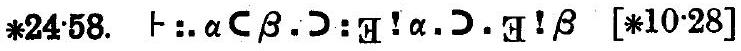
\includegraphics[max width=\textwidth, alt={}, center]{bc1848bf-39e8-4760-b069-9936044df683-100_51_741_1509_224}\\
＊246． F：$\alpha \subset \beta$ つ：$\alpha \neq \beta . \equiv$ ．$H!\beta-\alpha$\\
Dem．

\[
\begin{array}{ll}
\vdash \cdot * 22 \cdot 41 . \text { Transp. } & \supset \vdash: \mathrm{Hp} \cdot \supset: \alpha \neq \beta \cdot \supset \cdot \sim(\beta \subset \alpha) . \\
{[* 24 \cdot 55]} & \supset \cdot \text { H! } \beta-\alpha \\
\vdash . * 24 \cdot 21 . & \supset \vdash: \alpha=\beta \cdot \supset \cdot \beta-\alpha=\Lambda \\
\vdash .(2) \cdot \text { Transp } \cdot * 24 \cdot 54 \cdot \supset \vdash: \text { H! } \beta-\alpha \cdot \supset \cdot \alpha \neq \beta \\
\vdash .(1) \cdot(3) . & \supset \vdash \cdot \text { Prop } \tag{3}
\end{array}
\]

＊24．61． ト：$\sim$ H！$\beta$ ． ɔ ．$\alpha \cup \beta=\alpha$［ $* 24.51 \cdot 24$ ］\\
＊24．62．ト：$\sim$ Д！$\beta$. ɔ．$\alpha \cap \beta=\Lambda$［ $* 24.51$ ． 23 ］\\
*24.63. $\vdash: . \Lambda \sim \epsilon \kappa . \equiv: \alpha \in \kappa . \partial_{a}$. H! $\alpha$\\
In this proposition, the conditions of significance require that $\kappa$ should be a class of classes. The condition " $\alpha \in \kappa . \nu_{a} . \mathbb{H}!\alpha$ " is one required as hypothesis in many propositions. In virtue of the above proposition, this hypothesis may be replaced by " $\Lambda \sim \epsilon \kappa$."

Dem.

$$
\begin{array}{ll}
\vdash \cdot * 13 \cdot 191 \cdot \supset \vdash: . \Lambda \sim \epsilon \kappa & \equiv: \alpha=\Lambda \cdot \partial_{a} \cdot \alpha \sim \epsilon \kappa: \\
{[\text { Transp }]} & \equiv: \alpha \in \kappa \cdot \partial_{a} \cdot \alpha \neq \Lambda: \\
{[* 24 \cdot 54]} & \equiv: \alpha \in \kappa \cdot \partial_{a} \cdot \text { H }!\alpha: . \supset \vdash . \text { Prop }
\end{array}
$$

This proposition is frequently used in later parts of the work. We often have to deal with classes of existent classes, and the most convenient form in which to state that all the members of a class of classes exist is " $\Lambda \sim \in \boldsymbol{\epsilon}$."

\section*{＊25．THE UNIVERSAL RELATION，THE NULL RELATION，AND THE EXISTENCE OF RELATIONS}
Summary of＊25．\\
This number contains the analogues，for relations，of the definitions and propositions of $* 24$ ．Proofs will not be given，as they proceed precisely as in $* 24$ ．

The universal relation，denoted by $\dot{V}$ ，is the relation which holds between any two terms whatever of the appropriate types，whatever these may be in the given context．The null relation，$\dot{\Lambda}$ ，is the relation which does not hold between any pair of terms whatever，its type being fixed by the types of the terms concerning which the denial that it holds is significant．A relation $R$ is said to exist when there is at least one pair of terms between which it holds； ＂$R$ exists＂is written＂ $\mathbf{I}$ ！$R$ ．＂

The propositions of this number are much less often referred to than those of $* 24$ ，but for the sake of uniformity we have given the analogues of all propositions in $* 24$ ，with the same numeration（except for the integral part）．

All the remarks made in $* 24$ apply，mutatis mutandis，in the present number．\\
＊25．01．$\dot{\mathrm{V}}=\hat{x} \hat{y}(x=x . y=y) \quad$ Df\\
＊25．02．$\dot{\Lambda}=\dot{\mathrm{V}} \quad$ Df\\
＊25．03．安！$R .=.(\mathrm{H} x, y) . x R y$ Df\\
＊251．$\quad$ ．$\dot{\Lambda} \neq \dot{V}$\\
＊25－101． ㅅ．$\dot{V}=\dot{-} \dot{\Lambda}$\\
＊25•102． ！$:(x, y) \cdot \phi(x, y) \cdot \equiv . \hat{x} \hat{y} \phi(x, y)=\dot{\mathrm{V}}$\\
＊25•103． $\mathrm{F}:(x, y) \sim \phi(x, y) . \equiv . \hat{x} \hat{y} \phi(x, y)=\dot{\Lambda}$\\
＊25104．ト．$(x, y) . x \dot{V} y$\\
＊25－105．ㅏ．$(x, y) . \sim(x \dot{\Lambda} y)$\\
＊2511． ト．$(R) . R \in \mathrm{~V}$\\
＊2512． F．$(R) . \dot{\Lambda} \in R$\\
＊25－13． $\mathrm{F}: R=\dot{\Lambda} . \equiv R \subset \dot{\Lambda}$\\
＊2514． $\mathrm{F}:(x, y) . x R y . \equiv . R=\mathrm{V}$\\
＊25－141． F： V C $R . \equiv \mathrm{V}=R$\\
＊2515． ト $:(x, y) . \sim(x R y) . \equiv . R=\dot{\Lambda}$\\
＊2517． $\mathrm{F}: R=\dot{\mathrm{V}} . \equiv . \dot{-} R=\dot{\mathrm{\Lambda}}$\\
＊2521． ト $. R \dot{\circ}-R=\dot{\Lambda}$\\
＊25．22． F．$R \mho=R=\dot{\mathrm{V}}$\\
＊2523．ㄱ．$R \dot{\Lambda} \dot{\Lambda}=\dot{\Lambda}$\\
＊25．24． ＋．$R \cup \dot{\Lambda}=R$\\
＊2526． ト．$R \dot{\mathrm{~V}}=R$\\
＊2527． F．$R \mho \dot{\mathrm{~V}}=\dot{\mathrm{V}}$\\
＊25－3． $\mathrm{F}: R \in S . \equiv R \doteq S=\dot{\Lambda}$\\
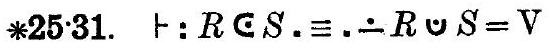
\includegraphics[max width=\textwidth, alt={}, center]{bc1848bf-39e8-4760-b069-9936044df683-103_49_551_510_125}\\
＊25311．$\vdash: R$ C－$S . \equiv R \dot{n} S=\dot{\Lambda}$\\
＊25312． $\mathrm{F}:-R \in S . \equiv R \cup S=\dot{\mathrm{V}}$\\
＊25313． $\mathrm{F}: R \dot{\circ} S=\dot{\Lambda} . \equiv R \cdots S=R$\\
＊2532． $\mathrm{F}: R \cup S=\dot{\Lambda} . \equiv . R=\dot{\Lambda} . S=\dot{\Lambda}$\\
＊25．33． $\mathrm{F}: R=\dot{\mathrm{V}} . \supset . R \circlearrowleft S=\dot{\mathrm{V}}$\\
＊2534．$f: R=\dot{\Lambda}$. ɔ.$R$ ก $S=\dot{\Lambda}$\\
＊2535． $\mathrm{F}: R=\dot{\mathrm{V}}$. ɔ $. R \dot{\cap} S=S$\\
＊2536． $\mathrm{F}: R=\dot{\Lambda}$. ɔ $. R \mho S=S$\\
＊2537． F $:: R \dot{\cap} S=\dot{\Lambda} . \equiv: . x R y . z S w . J_{x, y, z, w}: x \neq z . \vee . y \neq w$\\
＊25．38． $\mathrm{F}: . R \dot{n} S=\dot{\Lambda} . \supset: R \neq S$. v．$R=\dot{\Lambda} . S=\dot{\Lambda}$\\
＊25．39． $\mathrm{F}: R \dot{\circ} S=\dot{\Lambda} . \equiv: x R y . \nu_{x, y} \sim(x S y)$\\
＊254． F：$P \dot{\cap} Q=\dot{\Lambda} . \equiv(P \cup Q) \doteq P=Q . \equiv .(P \cup Q) \doteq Q=P$\\
＊25401． ᄀ ：$Q \subset P$ ．ɔ ．$(Q \cup R) \doteq P=R \doteq P$\\
＊25．402． । $: P \dot{\cap} Q=\dot{\Lambda} . R$ C $P . S \in Q$. ɔ $R \dot{n} S=\dot{\Lambda}$\\
＊2541． ト．$R=(R \dot{\circ} S) \cup(R-S)$\\
＊25411．$+: S \subset R$. ɔ $. R=S \cup(R-S)$\\
＊25．412． F ：$Q$ CP．SCQ．J．$(P \perp Q) \cup(Q-S)=P-S$\\
＊25．42． ㅣ：$P \dot{\circ} Q \subset R . P \ominus Q \subset R . \equiv P \subset R$\\
＊2543． ＊$: P \perp Q \subset R . \equiv P \in Q \cup R$\\
＊25－431．$F .(P \cup R) \dot{\wedge}(Q \cup \dot{-} R)=(P \dot{\cap} Q) \cup(P \doteq R) \cup(Q \dot{\wedge} R)$\\
＊25．432．$+(P \doteq R) \circlearrowleft(Q \dot{\cap} R)=(P \dot{\cap} Q) \mho(P \doteq R) \mho(Q \dot{\cap} R)$\\
＊25．44．$\quad$ … $(P \cup R) \dot{\cap}(Q \cup \dot{-} R)=(P \dot{\cap} \dot{-} R) \cup(Q \dot{\cap} R)$\\
＊25．45．$\quad \vdash:(P \dot{\cap} R) \circlearrowleft(Q-R)=\dot{\Lambda} . \equiv Q \in R . R \in-P$\\
＊25．46．$\vdash:(P \dot{\cap} R) \cup(Q \dot{-} R)=\dot{\Lambda} . \supset . P \dot{\cap} Q=\dot{\Lambda}$\\
＊25．47． F $: P \dot{\cap} Q=\dot{\Lambda} . P \cup Q=R . \equiv P \in R . Q=R \doteq P$\\
＊25．48．$\leqslant \therefore R \subset P . R^{\prime} \subset P . S \subset Q . S^{\prime} \subset Q . P \dot{\cap} Q=\dot{\Lambda} . \supset$ ：

$$
R \mho S=R^{\prime} \cup S^{\prime} . \equiv . R=R^{\prime} . S=S^{\prime}
$$

＊25．481．$+: . P \dot{\cap} Q=\dot{\Lambda} . P \dot{\cap} R=\dot{\Lambda} . \supset: P \circlearrowleft Q=P \circlearrowleft R . \equiv . Q=R$\\
＊25．482． ． ：$R$ C $P$ ．$S \subset Q . P \dot{\cap} Q=\dot{\Lambda} . \supset: R \circlearrowleft S=P \cup Q . \equiv R=P . S=Q$\\
＊25．49．ト：．$P \dot{\circ} Q=\dot{\Lambda} . \supset: P \in Q \cup R . \equiv . P \subset R$\\
＊25－491． $\mathrm{F}: Q \dot{\cap} R=\dot{\Lambda} . P \in Q \circlearrowleft R . \supset$ ．

$$
P \ominus Q=P \dot{\cap} R . P \ominus R=P \dot{\cap} Q . P=(P \doteq Q) \circlearrowleft(P \doteq R)
$$

＊25．492． न ：$Q \subset P . P \doteq Q=R . \supset . P \doteq R=Q$\\
＊25493． $\mathrm{F}: Q \dot{\circ} R=\dot{\Lambda}$ ．J．$P=(P \doteq Q) \cup(P \doteq R)$\\
＊25494．$F: R \in P . S \subset Q . P \dot{\cap} Q=\dot{\Lambda} . \supseteq .(R \cup S) \doteq P=S .(R \cup S) \doteq Q=R$\\
＊25495． $\mathrm{F}: P \dot{\cap} R=\dot{\Lambda}$. J．$(P \cup R) \dot{-}(Q \cup R)=P \dot{Q}$\\
＊255． $\mathrm{F}:$ 金！$R . \equiv .($ H $x, y) . x R y$\\
＊25．51．ト：～ที่！$R . \equiv . R=\dot{\Lambda}$\\
＊2552．ト．Hi！V்\\
＊2553．ト．～Η்！\\
＊25．54． ト：$\dot{\text { 且 }}$ ！$R \equiv$ ．$R \neq \dot{\Lambda}$\\
＊2555． ト：$\sim(R$ C $S)$ ．三丨由！$R$ ± $S$\\
＊2556． ト：．ぬ்！$(R$ c $S)$ ．三 ：पु ！R．v．千்！$S$\\

\includegraphics[max width=\textwidth, alt={}, center]{bc1848bf-39e8-4760-b069-9936044df683-104_46_611_854_202}\\
＊25．57． ト：$R$ ก $S=\Lambda$. つ：भु！$R$. J．$R$ \textbackslash ＃$S$\\
＊25．571．．ト：守！$R . R=S$. つ．守！$(R$ ก $S)$\\
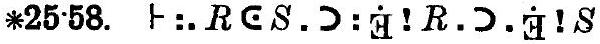
\includegraphics[max width=\textwidth, alt={}, center]{bc1848bf-39e8-4760-b069-9936044df683-104_44_600_1001_199}\\
＊256． ト：$R$ C $S$ ． J：$R$ 乘 $\equiv$ ．पु $!S \in R$\\
＊25．61． ト：～守！$S . \supset . R \cup S=R$\\
＊25．62． ト：～ทุ่！$S$. J．$R$ ก $S=\dot{\Lambda}$\\
＊25．63． ト $: . \dot{\Lambda} \sim \epsilon \kappa . \equiv: R \in \kappa . \partial_{R}$ ．守 $!R$

\section*{SECTION D}
\section*{LOGIC OF RELATIONS}
In the present section we shall be concerned with such of the general properties of relations as have no analogues in the theory of classes. The notations introduced in this section will be used constantly throughout the rest of the work, and the ideas expressed in the definitions will be found to be of fundamental importance.

\section*{*30. DESCRIPTIVE FUNCTIONS}
\section*{Summary of *30.}
The functions hitherto considered, with the exception of a few particular functions such as $\alpha \cap \beta$, have been propositional, i.e. have had propositions for their values. But the ordinary functions of mathematics, such as $x^{2}, \sin x$, $\log x$, are not propositional. Functions of this kind always mean "the term having such and such a relation to $x$." For this reason they may be called descriptive functions, because they describe a certain term by means of its relation to their argument. Thus " $\sin \pi / 2$ " describes the number 1; yet propositions in which $\sin \pi / 2$ occurs are not the same as they would be if 1 were substituted for $\sin \pi / 2$. This appears $e . g$. from the proposition " $\sin \pi / 2=1$," which conveys valuable information, whereas " $1=1$ " is trivial. Descriptive functions, like descriptions in general, have no meaning by themselves, but only as constituents of propositions*.

The general definition of a descriptive function is:

\section*{*30.01. $R^{6} y=(1 x)(x R y)$ Df}
That is, " $R^{\prime} y$ " is to mean "the term $x$ which has the relation $R$ to $y$." If there are several terms or none having the relation $R$ to $y$, all propositions about $R^{6} y$, i.e. all propositions of the form " $\phi\left(R^{6} y\right)$," will be false. The apostrophe in " $R^{6} y$ " may be read " of." Thus if $R$ is the relation of father to son, " $R^{\prime} y$ " means " the father of $y$." If $R$ is the relation of son to father, " $R^{6} y$ " means "the son of $y$ "; in this case, all propositions of the form " $\phi\left(R^{\prime} y\right)$ " will be false unless $y$ has one son and no more.

All the functions that occur in ordinary mathematics are instances of the above definition; all are obtained in the above manner from some relation. Thus in our notation " $R^{\prime} y$ " takes the place of what would commonly be "fy," this latter notation being reserved for propositional functions. We should write " $\sin$ ' $y$ " in place of " $\sin y$," using " $\sin$ " to express the relation of $x$ to $y$ when $x=\sin y$.

A definition such as $R^{\prime} y=(x)(x R y)$, where the meaning given to the term defined is a description, must be understood to mean that the term defined (in this case $R^{6} y$ ) and the description assigned as its meaning (in this case $(1 x)(x R y))$ are to be interchangeable in use: the definition is, in a sense, more purely symbolic than other definitions, since the description assigned as the meaning has itself no meaning except in use. It would perhaps be more formally correct to write

$$
\begin{gathered}
f\left(R^{6} y\right) .=. f\{(l x)(x R y)\} \text { Df. } \\
* \text { Cf. } * 14, \text { above. }
\end{gathered}
$$

But even this definition would not be quite complete, because it omits mention of the scope of the two descriptions. $R^{6} y$ and $(x)(x R y)$. Thus the complete form would be

$$
\left[R^{\prime} y\right] \cdot f\left(R^{\prime} y\right) \cdot=\cdot[(x)(x R y)] \cdot f\{(x x)(x R y)\} \text { Df. }
$$

But it is unnecessary to adopt this form of definition, provided it is understood that the definition $* 30 \cdot 01$ means that " $R^{6} y$ " may be written for " ( $\boldsymbol{a} \boldsymbol{x}$ ) ( $x R y$ )" everywhere, i.e. in indications of scope as well as elsewhere. The use of the definition occurs always in accordance with the proposition:

$$
\vdash:\left[R^{\prime} y\right] \cdot f\left(R^{\prime} y\right) \cdot \equiv \cdot[(\imath x)(x R y)] \cdot f(\imath x)(x R y),
$$

which is $* 30 \cdot 1$, below.\\
It is to be observed that $* 30.01$ does not necessarily involve

$$
R^{\prime} y=(x x)(x R y) .
$$

For this, by the definition, is equivalent to

$$
(x x)(x R y)=(x)(x R y),
$$

which, by $* 14 \cdot 28$, only holds when $\mathrm{E}!(x)(x R y)$, i.e. when there is one term, and no more, which has the relation $R$ to $y$.

All the conventions as to scope explained in $\boldsymbol{*} \mathbf{1 4}$ are to be transferred to $R^{\prime} x$, i.e., in the absence of any contrary indication, the scope of $R^{\prime} x$ is to be the smallest proposition, enclosed in dots or other brackets, in which the $R^{6} x$ in question occurs.

We put\\
*30.02. $R^{6} S^{6} y=R^{6}\left(S^{6} y\right)$ Df\\
This definition serves merely for the avoidance of brackets. It is to be interpreted as meaning

$$
\left[R^{6} S^{6} y\right] \cdot f\left(R^{6} S^{6} y\right) \cdot=\cdot\left[R^{6}\left(S^{6} y\right)\right] \cdot f\left\{R^{6}\left(S^{6} y\right)\right\} \quad \text { Df. }
$$

In future, we shall often define a new expression as having a descriptive phrase for its meaning; in such a case, the definition is always to be interpreted as above. That is, any proposition in which the new expression occurs is to be the proposition which is obtained by substituting the old expression for the new one wherever the latter occurs.\\
$R^{\prime}\left(S^{\prime} y\right)$, in the above, is to be interpreted by first treating $S^{6} y$ as if it were not a descriptive symbol, and applying $* 30.01$ and $* 14.01$ or $* 14.02$ to $R^{6}\left(S^{6} y\right)$, and by then applying $* 30.01$ and $* 14.01$ or $* 1402$ to $S^{6} y$.

The majority of the propositions of the present number are immediate consequences of the corresponding propositions in *14. Thus *14:31-34 and $* 14 \cdot 113$ lead immediately to $* 30 \cdot 12-16$, which show that, either always or when $R^{\prime} y$ exists, the "scope" of $R^{\prime} y$ or of $R^{\prime} y$ and $S^{\prime} y$ makes no difference to the truth-values of such propositions as we are concerned with. We have *30-18. $\vdash: . \mathrm{E}!R^{6} y:(z) . \phi z:$ ɔ.$\phi\left(R^{6} y\right)$\\
so that what holds of everything holds of $R^{6} y$ ，provided $R^{6} y$ exists．This results immediately from $* 1418$ ，and shows that，provided $R^{6} y$ exists，the fact that＂$R^{6} y$＂is an incomplete symbol does not prevent its being substituted as a value of $z$ whenever we have $(z) \cdot \phi z$ ，or an assertion of the propositional function $\phi z$ ．

One of the most used propositions of this number is：\\
＊303． $\mathrm{F}: . x=R^{6} y . \equiv: z R y . \equiv_{z} . z=x$\\
which results immediately from $* 14202$ ．The following analogous proposition results from the above by means of $* 14 \cdot 122$ ：\\
＊3031．$\vdash: . x=R^{\prime} y . \equiv: x R y: z R y . \partial_{z} . z=x$\\
I．e．＂$x=R^{6} y$＂involves，in addition to＂$x R y$ ，＂the statement that what－ ever has the relation $R$ to $y$ is identical with $x$ ．

A proposition constantly referred to is：\\
＊3037．$\leqslant \mathrm{E}!R^{6} y \cdot y=z \cdot$ ɔ $\cdot R^{6} y=R^{6} z$\\
In the hypothesis， $\mathrm{E}!R^{6} y$ might be replaced by $\mathrm{E}!R^{6} z$ ，but one or other of them is essential．For，by $* 1421$ ，＂$R^{6} y=R^{6} z$＂implies $\mathrm{E}!R^{6} y$ and $\mathrm{E}!R^{6} z$ （these are equivalent when $y=z$ ），and therefore cannot be true when $R^{6} y$ and $R^{6} z$ do not exist．

The use of＊30．37 is chiefly in cases where $y$ or $z$ or both are replaced by descriptive functions．Suppose，for example，that $z$ is replaced by $S^{6} w$ ．By $* 30 \cdot 18$ ，we may substitute $S^{6} w$ for $z$ if $S^{6} w$ exists．By $* 14 \cdot 21$ ，both sides of the implication in $* 30.37$ will become false if $S^{6} w$ does not exist，and there－ fore the implication will still hold．Hence whether $S^{6} w$ exists or not，we may substitute it for $z$ and obtain

$$
\text { ト: E }!R^{6} y \cdot y=S^{6} w \cdot \supset \cdot R^{6} y=R^{6} S^{6} w
$$

In like manner，if we replace $y$ by $T^{c} v$ ，we obtain

$$
\text { 卜:E! } R^{6} T^{6} v \cdot T^{6} v=S^{6} w \cdot \supset \cdot R^{6} T^{6} v=R^{6} S^{6} w
$$

A very important proposition is ：\\
＊304． ト： $\mathrm{E}!R^{6} y$ ．$\supset: a=R^{6} y$ ．$\equiv a R y$\\
This proposition states that，provided $R^{6} y$ exists，to say that $a$ is the term which has the relation $R$ to $y$ is equivalent to saying that $a$ has the relation $R$ to $y$ ．Thus for example＂$a$ is the occupier of the house $y$＂is equivalent to＂$a$ occupies the house $y$ ，＂＂$a$ is the writer of Waverley＂is equivalent to ＂$a$ wrote Waverley，＂＂$a$ is the father of $y$＂is equivalent to＂$a$ begot $y$ ．＂But we cannot argue from＂John Smith inhabits London＂to＂John Smith is the inhabitant of London．＂

We shall introduce in this and subsequent sections many constant relations for which $\mathrm{E}!R^{6} y$ is always true．When $R$ is such that $\mathrm{E}!R^{6} y$ is always true， we have，in virtue of $* 30 \cdot 4$ ，

$$
a=R^{\prime} y \cdot \equiv \cdot a R y
$$

for every possible value of $y$. The following proposition is useful in cases where both $R$ and $S$ are such that $R^{6} y$ and $S^{6} y$ always exist:\\
*3041. F: $(y) \cdot R^{6} y=S^{6} y \cdot \equiv:(y) \cdot \mathrm{E}!R^{6} y: R=S$\\
Thus if we know that $R^{c} y$ and $S^{c} y$ are always identical, we know not only that $R$ and $S$ are identical, but also that $R^{c} y$ (and therefore $S^{c} y$ ) always exists.\\
*30.01. $R^{\prime} y=(x x)(x R y)$ Df\\
*30.02. $R^{6} S^{6} y=R^{6}\left(S^{6} y\right)$ Df\\
In interpreting $R^{c}\left(S^{c} y\right), S^{c} y$ is to be treated as an ordinary symbol until $R^{6}\left(S^{6} y\right)$ has been eliminated by $* 30.01$ and $* 14.01$ or $* 14.02$, and then the above definitions are to be applied to $S^{6} y$.\\
*30.1. $\quad \vdash:\left[R^{\prime} y\right] \cdot f\left(R^{\prime} y\right) \cdot \equiv \cdot[(x x)(x R y)] \cdot f(x x)(x R y) \quad[* 4 \cdot 2 \cdot(* 30 \cdot 01)]$\\
*30•11. $\vdash:\left[R^{\prime} y\right] \cdot f\left(R^{\prime} y\right) \cdot \equiv:\left(\mathrm{H}^{b}\right): x R y \cdot \equiv_{x} \cdot x=b: f b[* 30 \cdot 1 \cdot * 14 \cdot 1]$\\
The following propositions are immediate applications of *14.31 ff., made in accordance with $* 30 \cdot 1$.\\
*30-12. $+:: \mathrm{E}!R^{6} y, \partial:\left[R^{6} y\right], p \vee \chi\left(R^{6} y\right) . \equiv: p . \vee .\left[R^{6} y\right] . \chi\left(R^{6} y\right)$\\[0pt]
[*14:31]\\
*30-13. $\vdash:: \mathrm{E}!R^{\prime} y$. J: $\left[R^{\prime} y\right] . \sim \chi\left(R^{\prime} y\right) . \equiv \sim\left\{\left[R^{\prime} y\right] \cdot \chi\left(R^{\prime} y\right)\right\} \quad[* 14: 32]$\\
*30-14. $+:: \mathrm{E}!R^{6} y . \supset:\left[R^{6} y\right] \cdot p \supset \chi\left(R^{6} y\right) \cdot \equiv: p \cdot \supset \cdot\left[R^{6} y\right] \cdot \chi\left(R^{6} y\right)$ [*14:33]\\
*30-141. $+:: \mathrm{E}!R^{6} y \cdot \supset: \cdot\left[R^{6} y\right] \cdot \chi\left(R^{6} y\right) \supset p \cdot \equiv:\left[R^{6} y\right] \cdot \chi\left(R^{6} y\right) \cdot \supset \cdot p$ [*14:331]\\
*30-142. +:: $\mathrm{E}!R^{6} y$. J:. $\left[R^{6} y\right] . p \equiv \chi\left(R^{6} y\right) . \equiv: p . \equiv .\left[R^{6} y\right] \cdot \chi\left(R^{6} y\right)$\\[0pt]
[*14:332]\\
*30-15. F $:, p:\left[R^{\prime} y\right] \cdot \chi\left(R^{\prime} y\right): \equiv:\left[R^{\prime} y\right] \cdot p \cdot \chi\left(R^{\prime} y\right)[* 1434]$\\
The following two propositions are immediate consequences of $* 14 \cdot 113 \cdot 112$.\\
*30.16. ! : $\left[R^{6} y\right] \cdot f\left(R^{6} y, S^{6} z\right) \cdot \equiv \cdot\left[S^{6} z\right] \cdot f\left(R^{6} y, S^{6} z\right)[* 14 \cdot 113]$\\
*30-17. $\vdash: .\left[R^{6} y\right] . f\left(R^{6} y, S^{6} z\right) . \equiv:$\\
( $\mathrm{H}^{b, c}$ ) $: x R y . \equiv_{x} . x=b: x S z . \equiv_{x} . x=c: f(b, c)[$ *14:112]\\
*30-18. $\vdash: \mathrm{E}!R^{6} y:(z) \cdot \phi z:$ ɔ $\cdot \phi\left(R^{6} y\right)$ [*14•18]\\
*3019. $\left.\vdash: R^{6} y=b.\right): \psi\left(R^{6} y\right) . \equiv . \psi b$ [*14.15]\\
*302. F:. E! $R^{6} y . \equiv:\left(\mathrm{H}^{b}\right): x R y . \equiv_{x} . x=b[* 4 \cdot 2 . * 14 \cdot 11 .(* 30.01)]$\\
In proving $* 30 \cdot 2$, we have to use the definition $* 30 \cdot 01$, not $* 30 \cdot 1$, because $\mathrm{E}!(x)(\phi x)$ is not of the form $f(x)(\phi x)$. This appears if we attempt to apply the definition $* 1401$ to $\mathbf{E}!(x)(\phi x)$, which leads to an expression containing the meaningless constituent $\mathrm{E}!b$. But by the definition $* 30 \cdot 01$, every typographical occurrence of the symbol " $R^{6} y$ " means what results when this symbol is replaced by " $(x)(x R y)$," hence " $\mathrm{E}!R^{\prime} y$ " means " $\mathrm{E}!(x x)(x R y)$."\\
$* 3021 . \vdash:: \mathrm{E}!R^{6} y . \equiv:(\mathrm{H} x) . x R y: x R y . z R y . \partial_{x, z} . x=z$ ［＊14•203．（＊30．01）］\\
＊3022． $\mathrm{F}: \mathrm{E}!R^{\prime} y . \equiv R^{\prime} y=(1 x)(x R y)[* 14 \cdot 28 .(* 30 \cdot 01)]$\\
Note that we do not necessarily have

$$
R^{\prime} y=(\imath x)(x R y),
$$

which is only true when $\mathrm{E}!R^{6} y$ ．\\
＊303． $\mathrm{F}: . x=R^{6} y . \equiv: z R y . \equiv_{z} . z=x \quad$［＊14202］\\
＊3031．$\vdash: . x=R^{6} y . \equiv: x R y: z R y . D_{z} . z=x$［＊14．122．＊30．3］\\
＊3032． $\mathrm{F}: \mathrm{E}!R^{6} y . \equiv\left(R^{6} y\right) R y$［＊14：22］\\
＊3033．$\vdash:: \mathrm{E}!R^{6} y \cdot \supset:, \psi\left(R^{6} y\right): \equiv:(\mathbb{H} x) \cdot x R y \cdot \psi x: \equiv: x R y \cdot \nu_{x} \cdot \psi x$\\
［＊14：26］\\
＊3034．$\vdash: x R y . \equiv_{x} . x S y:$ J：E：$R^{6} y . \equiv . \mathrm{E}!S^{6} y$［＊14＇271］\\
＊30341． r：$x R y$ ．$\equiv_{x} . x S y:$ J：E $!R^{6} y . \equiv R^{6} y=S^{6} y$\\
Dem．


\begin{align*}
& \text { ト. } * 1421 . \quad \supset \vdash: R^{6} y=S^{6} y . \text { ɔ.E! } R^{6} y  \tag{1}\\
& \text { ト. *14:27. Comm . ɔ : . Hp. ɔ : E ! } R^{c} y . \supset . R^{c} y=S^{c} y  \tag{2}\\
& \text { ト.(1).(2). ɔㄴ.Prop }
\end{align*}


＊3035． $\mathrm{F}: . R=S . \mathrm{J}: \mathrm{E}!R^{6} y . \equiv . \mathrm{E}!S^{6} y[* 3034 . * 21 \cdot 43]$\\
＊3036．$\vdash: \mathrm{E}!R^{6} y . R=S . \supset . R^{6} y=S^{6} y \quad$［＊14－27．Imp．＊2143］\\
＊30．37．$\vdash: \mathrm{E}!R^{6} y \cdot y=z \cdot$ J．$R^{6} y=R^{6} z$\\
Dem．

\[
\begin{array}{ll}
\vdash \cdot * 14 \cdot 28 . & \supset \vdash: \mathrm{E}: R^{6} y \cdot \supset \cdot R^{6} y=R^{6} y \\
\vdash \cdot * 13 \cdot 12 . & \supset \vdash: y=z \cdot \supset: R^{6} y=R^{6} y \cdot \equiv R^{6} y=R^{6} z  \tag{2}\\
\vdash \cdot(1) \cdot(2) \cdot \text { Ass } . \text { つ } \cdot \text { Prop }
\end{array}
\]

This proposition is very frequently used．\\
＊304．$\quad \vdash: \mathrm{E}!R^{\prime} y$. J $: a=R^{\prime} y . \equiv$ aRy［＊14：241］\\
This is a very important proposition，of which the use is constant．\\
＊3041．F：．$(y) \cdot R^{6} y=S^{6} y \cdot \equiv:(y) \cdot \mathrm{E}!R^{6} y: R=S$\\
Dem．\\
ト．$* 1421 . * 10 \cdot 11 \cdot 27$. つト：$(y) . R^{6} y=S^{6} y$. ɔ．$(y) . E!R^{6} y$

ト．＊14•13•142．$\quad \supset+:(y) \cdot R^{\prime} y=S^{\prime} y \cdot \supset:(x, y): x=R^{\prime} y \cdot \equiv \cdot x=S^{\prime} y$ ：\\
［（1）＊304］$\supset:(x, y): x R y . \equiv . x S y:$\\
［＊21•43］$\supset: R=S$

ト．＊3036．$\quad \supset \vdash: \mathrm{E} u R^{\prime} y, R=S . \supset . R^{\prime} y=S^{\prime} y$ ：\\
［＊10．11．27．35］ɔト：．$(y) . \mathrm{E}!R^{6} y: R=S: \supset .(y) . R^{6} y=S^{6} y$

ト．（1）．（2）．（3）．ɔ…Prop\\
＊3042．$+:(y) . \mathrm{E}!R^{c} y . \supset:(y) . R^{c} y=S^{c} y . \equiv . R=S$［＊30：41］\\
The hypothesis $(y) \cdot \mathrm{E}!R^{\prime} y$ is fulfilled by a number of important special relations，of which examples will occur in the subsequent numbers of the present section．\\
＊305．ト：E！PrQcz．J．E！Q6z\\
Dem．

$$
\begin{array}{ll}
\vdash \cdot * 30 \cdot 2 . \text { つ! }: \mathrm{E}: P^{6} Q^{6} z . \equiv:\left(\mathrm{H}^{b}\right): x P\left(Q^{6} z\right) \cdot \equiv_{x} \cdot x=b: \\
{[* 10 \cdot 1]} & \supset:\left(\mathrm{H}^{b}\right): b P\left(Q^{6} z\right) \cdot \equiv b=b: \\
{[* 13 \cdot 15]} & \supset:\left(\mathrm{H}^{b}\right) \cdot b P\left(Q^{6} z\right): \\
{[* 14 \cdot 21]} & \supset: \mathrm{E}!Q^{6} z: \text { J } . \text { Prop }
\end{array}
$$

＊30501．$+: \phi\left(P^{6} Q^{6} z\right)$ ．こ．（马 $\left.b, c\right) \cdot c=Q^{6} z \cdot b=P^{6} c \cdot \phi b$\\
On the meaning of＂$\phi\left(P^{\prime} Q^{\prime} z\right)$ ，＂see note to the definition $* 3002$ ．\\
Dem．\\
$\vdash . * 14 \cdot 1 \cdot 122$. つ $:: \phi\left(P^{6} Q^{6} z\right) . \equiv:\left(g^{b}\right): b P\left(Q^{6} z\right): x P\left(Q^{6} z\right) . \partial_{x} . x=b: \phi b:$.\\
［＊14：205］． $\equiv:\left(H^{b}\right):\left(H^{c}\right): c=Q^{6} z: b P c: x P c . \partial_{x} . x=b: \phi b:$.\\
［＊14•122•202］ $\equiv:\left(\mathrm{H}^{b}, c\right) . c=Q^{c} z . b=P^{c} c . \phi b:: \supset F$ ．Prop\\
＊30．51．$f: b=P^{6} Q^{6} z . \equiv .\left(\mathrm{G}^{c}\right) . b=P^{6} c . c=Q^{6} z \quad[* 30.501 . * 13.195]$\\
＊3052． $\mathrm{F}: \mathrm{E}!P^{6} Q^{6} z . \equiv .\left(\mathrm{g}^{b}, c\right) . b=P^{6} c . c=Q^{6} z[* 30.51 . * 14 \cdot 204]$

\section*{*31. CONVERSES OF RELATIONS}
\section*{Summary of *31.}
If $R$ is a relation, the relation which $y$ has to $x$ when $x R y$ is called the converse of $R$. Thus greater is the converse of less, before of after, husband of wife. The converse of identity is identity, and the converse of diversity is diversity. The converse of $R$ is written $\breve{R}$ (read " $R$-converse"). When $R=\breve{R}, R$ is called a symmetrical relation, otherwise it is called not-symmetrical. When $R$ is incompatible with $\breve{R}, R$ is called asymmetrical. Thus "cousin" is symmetrical, "brother" is not-symmetrical (because when $x$ is the brother of $y, y$ may be either the brother or the sister of $x$ ), and "husband" is asymmetrical.

The relation of $\breve{R}$ to $R$ is called "Cnv." It will be shown that every relation has one, and only one, converse; hence, applying the notation of $* 30$, that one is $\operatorname{Cnv}^{\prime} R$. Thus $\breve{R}=\operatorname{Cnv}^{\prime} R$. We have thus two notations for the converse of $R$; the second is more convenient for the converse of a relation not denoted by a single letter.

The more important propositions of the present number are the following:

\section*{*31-13. +. E!Cnv' $P$}
I.e. any relation $P$ has a converse. Hence the relation "Cnv" verifies the hypothesis $(y) . \mathrm{E}!R^{6} y$, i.e. we have $(P) . \mathrm{E}!\mathrm{Cnv}^{6} P$.\\
*3132. $F: P=Q . \equiv . \breve{P}=\breve{Q}$\\
I.e. two relations are identical when, and only when, their converses are identical.\\
*3133. $\quad$. $\mathrm{Cnv}^{\prime} \mathrm{Cnv}^{\prime} P=P$\\
I.e. any relation is the converse of its converse.

Very many of the subsequent uses of the notion of the converse of a relation require only the propositions which embody the definitions of $\breve{P}$ and Cnv, namely\\
\textit{31}11. * : $x \breve{P} y$. $\equiv . y P x$\\
and\\
*31-131. $\cdot: x\left(\mathrm{Cnv}^{\prime} P\right) y . \equiv . y P x$\\
*31.01. $\mathrm{Cnv}=\hat{Q} \hat{P}\left\{x Q y . \equiv_{x, y \cdot y} P x\right\}$. Df\\
*31.02. $\breve{P}=\hat{x} \hat{y}(y P x) \quad$ Df\\
*31•1. F:. $Q \operatorname{Cnv} P . \equiv: x Q y . \equiv_{x, y \cdot y P x} \quad[* 21 \cdot 3 .(* 31 \cdot 01)]$\\
*31.101. F: $Q \operatorname{Cnv} P . R \operatorname{Cnv} P . \supset . Q=R$\\
Dem.

$$
\begin{array}{ll}
\vdash \cdot * 31 \cdot 1 . \supset \vdash: . \mathrm{Hp} . & \supset: x Q y . \equiv_{x, y} \cdot y P x: x R y . \equiv_{x, y} \cdot y P x: \\
{[* 11 \cdot 371]} & \supset: x Q y . \equiv_{x, y} \cdot x R y: \\
{[* 21 \cdot 43]} & \supset: Q=R:, \supset \vdash . \text { Prop }
\end{array}
$$

*31.11. $F: x \breve{P} y . \equiv . y P x$ [*21.3.(*31.02)]\\
*31.111. ト. $\breve{P} \operatorname{Cnv} P$ [*31.111]\\
*3112. ト $. \breve{P}=\mathrm{Cnv}^{\prime} P$\\
Dem.


\begin{align*}
& \vdash \cdot * 31 \cdot 101 \cdot \supset \vdash: Q \operatorname{Cnv} P \cdot \breve{P} \operatorname{Cnv} P \cdot \supset \cdot Q=\breve{P}: \\
& {[* 31 \cdot 111] \quad \supset \vdash: Q \operatorname{Cnv} P \cdot \supset \cdot Q=\breve{P}}  \tag{1}\\
& \text { F.(1).*10.11.*31.111.} \supset \\
& \quad \vdash: \breve{P} \operatorname{Cnv} P: Q \operatorname{Cnv} P \cdot \partial_{Q} \cdot Q=\breve{P}: \\
& {[* 30 \cdot 31] \quad \supset \vdash \cdot \breve{P}=\operatorname{Cnv}^{\prime} P}
\end{align*}


*31.13. F. E! Cnv' $P$ [*14.21.*31.12]\\
*31•131. $\vdash: x\left(\mathrm{Cnv}^{\prime} P\right) y . \equiv . y P x \quad$ [*31•11•12•*21•43]\\
*31•132. $F: Q \operatorname{Cnv} P . \equiv Q=\operatorname{Cnv}^{\mathrm{c}} P . \equiv . Q=\breve{P} \quad[* 30 \cdot 4 . * 31 \cdot 13 \cdot 12]$\\
*3114. $\quad \vdash . \mathrm{Cnv}^{\mathrm{c}}(P \dot{\cap} Q)=\mathrm{Cnv}^{\mathrm{c}} P \dot{\cap} \mathrm{Cnv}^{\mathrm{c}} Q$\\
Dem.

\[
\begin{array}{ll}
\vdash . * 31 \cdot 131 . \supset \vdash: x\left\{\mathrm{Cnv}^{6}(P \dot{\circ} Q)\right\} y & \equiv . y(P \dot{\circ} Q) x . \\
{[* 21 \cdot 33]} & \equiv . y P x . y Q x . \\
{[* 31 \cdot 131]} & \equiv . x\left(\mathrm{Cnv}^{6} P\right) y . x\left(\mathrm{Cnv}^{6} Q\right) y . \\
{[* 21 \cdot 33]} & \equiv . x\left\{\mathrm{Cnv}^{6} P \dot{\circ} \mathrm{Cnv}^{6} Q\right\} y  \tag{1}\\
\vdash .(1) . * 11 \cdot 11 . * 21 \cdot 43 . \supset \vdash . \text { Prop } &
\end{array}
\]

*3115. F. $\mathrm{Cnv}^{\prime}(P \cup Q)=\mathrm{Cnv}^{\prime} P \cup \mathrm{Cnv}^{\prime} Q$ [Similar proof]\\
*3116. $\vdash . \mathrm{Cnv}^{\prime} \doteq P=\dot{-}\left(\mathrm{Cnv}^{\prime} P\right)$\\
Dem.

\[
\begin{array}{ll}
\vdash \cdot * 31 \cdot 131 \cdot \supset \vdash: x\left(\mathrm{Cnv}^{6}+P\right) y & \equiv \cdot y \doteq P x \\
{[* 23 \cdot 35]} & \equiv \sim \sim(y P x) \\
{[* 31 \cdot 131]} & \equiv \sim \sim\left\{x\left(\mathrm{Cnv}^{4} P\right) y\right\} \\
{[* 23 \cdot 35]} & \equiv . x\left\{-\left(\mathrm{Cnv}^{4} P\right)\right\} y  \tag{1}\\
\vdash \cdot(1) \cdot * 11 \cdot 11 \cdot * 21 \cdot 43 . \supset \vdash . \text { Prop }
\end{array}
\]

＊31．17．$+: . y=\breve{P}^{\prime} x . \equiv: x P z . \equiv_{z} . z=y \quad[* 30 \cdot 3 . * 31 \cdot 11]$\\
＊31．18．$+: . \mathrm{E}!\breve{P}^{6} x . \equiv:(\mathrm{H} y): x P z . \equiv_{z} . z=y$［＊30．2．＊31．11］\\
＊3121．ㄱ． $\mathrm{Cnv}^{\prime} \dot{\Lambda}=\dot{\Lambda}$\\
Dem．


\begin{align*}
& \vdash \cdot * 31 \cdot 131 . \supset f: x\left(\mathrm{Cnv}^{\top} \dot{\Lambda}\right) y . \equiv . y \dot{\Lambda} x: \\
& {[* 25 \cdot 105] \quad \supset \vdash . \sim x\left(\mathrm{Cnv}^{\top} \dot{\Lambda}\right) y}  \tag{1}\\
& \vdash .(1) \cdot * 11 \cdot 11 \cdot * 25 \cdot 15 . \supset \vdash . \text { Prop }
\end{align*}


＊31．22．$\quad$ ‥ $\mathrm{Cnv} \vee \dot{\mathrm{V}}=\dot{\mathrm{V}} \quad$［Similar proof］\\
＊3123． $\mathrm{F}: \breve{P}=\dot{\mathrm{V}} . \equiv P=\dot{\mathrm{V}}$\\
Dem．

$$
\begin{array}{ll}
\vdash \cdot * 25 \cdot 14 \cdot \supset \vdash: \breve{P}=\dot{\mathrm{V}} . & \equiv(x, y) \cdot x \breve{P} y \\
{[* 31 \cdot 11 \cdot * 11 \cdot 33]} & \equiv \cdot(x, y) \cdot y P x \\
{[* 11 \cdot 2]} & \equiv \cdot(y, x) \cdot y P x \\
{[* 25 \cdot 14]} & \equiv \cdot P=\dot{\mathrm{V}}: \supset \vdash . \text { Prop }
\end{array}
$$

＊31．24 $f: \breve{P}=\dot{\Lambda} . \equiv . P=\dot{\Lambda} \quad$［Similar proof］\\
＊31．32． F：$P=Q . \equiv . \breve{P}=\breve{Q}$\\
Dem．

$$
\begin{array}{ll}
\vdash \cdot * 21 \cdot 43 \cdot \supset \vdash: . P=Q \cdot & \equiv: x P y \cdot \equiv_{x, y} \cdot x Q y: \\
{[* 4 \cdot 86 \cdot 21 \cdot * 31 \cdot 11]} & \equiv: y \breve{P}_{x} \cdot \Xi_{x, y} \cdot y \stackrel{\breve{Q}}{x}: \\
{[* 11 \cdot 2]} & \stackrel{\equiv}{y \breve{P} x} \cdot \equiv_{y, x} \cdot y \breve{Q} x: \\
{[* 21 \cdot 43]} & \equiv: \breve{P}=\breve{Q}: . \supset \vdash . \text { Prop }
\end{array}
$$

＊3133． $\mathrm{F} . \mathrm{Cnv}^{\prime} \mathrm{Cnv}^{\prime} P=P$\\
Dem．


\begin{align*}
& \vdash \cdot * 31 \cdot 131 \cdot \text { つト: } x\left(\mathrm{Cnv}^{4} \mathrm{Cnv}^{4} P\right) y \equiv . y\left(\mathrm{Cnv}^{6} P\right) x . \\
& \equiv x P y  \tag{1}\\
& {[* 31 \cdot 131] }=x . \\
& \vdash \cdot(1) \cdot * 11 \cdot 11 \cdot * 21 \cdot 43 . \text { ɔ } . \text { Prop }
\end{align*}


＊3134． $\mathrm{F}: P=\breve{Q} \cdot \equiv \cdot Q=\breve{P}$\\
Dem．

$$
\begin{array}{ll}
\vdash \cdot * 31 \cdot 32 . \supset \vdash: P=\breve{Q} . \equiv . \breve{P} & =\mathrm{Cnv}^{v} \breve{Q} \\
{[* 31 \cdot 12 \cdot 32]} & =\mathrm{Cnv}^{v} \mathrm{Cnv}^{v} Q \\
{[* 31 \cdot 33]} & =Q: \supset \vdash . \text { Prop }
\end{array}
$$

＊314．$\quad \vdash: P \in Q . \equiv . \breve{P} \in \breve{Q} \quad[* 31 \cdot 11 . * 11 \cdot 33]$\\
＊3141．$\quad \vdash: P \in \breve{Q} . \equiv \breve{P} \in Q \quad$［＊31•433•12］\\
＊315． ト：守！$P$ ．$\equiv$ 守！$\breve{P}$［＊31•24．Transp．＊25•54］\\
*31.51. $\vdash:(P) \cdot \overrightarrow{f P} \cdot \equiv \cdot(P) \cdot f P$\\
Dem.


\begin{align*}
& \forall \cdot * 10 \cdot 1 . \supset \vdash:(P) \cdot f P \cdot \supset \cdot f \breve{P}: \\
& {[* 10 \cdot 11 \cdot 21] } \supset \vdash:(P) \cdot f P \cdot \supset \cdot(P) \cdot f \breve{P}  \tag{1}\\
&+\cdot * 10 \cdot 1 \cdot * 31 \cdot 12 \cdot \supset \\
&+:(P) \cdot f \breve{P} \cdot \supset \cdot f\left(\mathrm{Cnv}^{6} \breve{P}\right) . \\
& {[* 31 \cdot 33 \cdot 12] \quad } \supset \cdot f P: \\
& {[* 10 \cdot 11 \cdot 21] \supset+:(P) \cdot f \breve{P} \cdot \supset \cdot(P) \cdot f P }  \tag{2}\\
&+\cdot(1) \cdot(2) \cdot \supset+\cdot \operatorname{Prop}
\end{align*}


*31.52. $\vdash:\left(\frac{H}{P}\right) \cdot f \breve{P} \cdot \equiv \cdot(H P) \cdot f P$ [*31.51.Transp]

\section*{*32. REFERENTS AND RELATA OF A GIVEN TERM WITH RESPECT TO A GIVEN RELATION}
\section*{Summary of *32.}
Given any relation $R$, the class of terms which have the relation $R$ to a given term $y$ are called the referents of $y$, and the class of terms to which a given term $x$ has the relation $R$ are called the relata of $x$. We shall denote by $\vec{R}$ the relation of the class of referents of $y$ to $y$, and by $\overleftarrow{R}$ the relation of the class of relata of $x$ to $x$. It is convenient also to have a notation for the relations of $\vec{R}$ and $\overleftarrow{R}$ to $R$. We shall denote the relation of $\vec{R}$ to $R$ by "sg," where "sg" stands for "sagitta." Similarly we shall denote by "gs" the relation of $\overleftarrow{R}$ to $R$, to suggest an arrow running from right to left instead of from left to right. $\vec{R}$ and $\overleftarrow{R}$ are chiefly useful for the sake of the descriptive functions to which they give rise; thus $\vec{R}^{\prime} y=\hat{x}(x R y)$ and $\overleftarrow{R}^{\prime} x=\hat{y}(x R y)$. Thus e.g. if $R$ is the relation of parent to son, $\vec{R}^{\prime} y=$ the parents of $y, \overleftarrow{R}^{\prime} x=$ the sons of $x$. If $R$ is the relation of less to greater among numbers of any kind, $\vec{R}^{\prime} y=$ numbers less than $y$, and $\overleftarrow{R}^{\prime} x=$ numbers greater than $x$. When $R^{\prime} y$ exists, $\vec{R}^{\prime} y$ is the class whose only member is $R^{6} y$. But when there are many terms having the relation $R$ to $y, \vec{R}^{\prime} y$, which is the class of those terms, supplies a notation which cannot be supplied by $R^{\prime} y$. And similarly if there are many terms to which $x$ has the relation $R, \overleftarrow{R}^{\prime} x$ supplies the notation for these terms. Thus for example let $R$ be the relation "sin," i.e. the relation which $x$ has to $y$ when $x=\sin y$. Then " $\sin ^{6} x$ " represents all values of $y$ such that $x=\sin y$, i.e. all values of $\sin ^{-1} x$ or $\arcsin x$. Unlike the usual symbol, it is not ambiguous, since instead of representing some one of these values, it represents the class of them.

The definitions of $\vec{R}, \overleftarrow{R}$, sg, gs are as follows:\\
*32.01. $\vec{R}=\hat{a} \hat{y}\{\alpha=\hat{x}(x R y)\} \quad$ Df\\
*32.02. $\overleftarrow{R}=\hat{\beta} \hat{x}\{\beta=\hat{y}(x R y)\} \quad$ Df\\
*32.03. $\mathrm{sg}=\hat{A} \hat{R}(A=\vec{R}) \quad$ Df\\
*32.04. $\mathrm{gs}=\hat{A} \hat{R}(A=\overleftarrow{R}) \quad$ Df\\
In virtue of the above definitions, we shall have $\operatorname{sg}^{6} R=\vec{R}, \operatorname{gs}^{6} R=\overleftarrow{R}$. This gives an alternative notation which is convenient in dealing with a relation not represented by a single letter.

It should be observed that if $R$ is a homogeneous relation (i.e. one in which referents and relata are of the same type), then $\vec{R}$ and $\overleftarrow{R}$ are not homogeneous, but relate a class to objects of the type of its members.

In virtue of the definitions of $\vec{R}$ and $\overleftarrow{R}$, we shall have


\begin{equation*}
\vdash \cdot \vec{R}^{6} y=\hat{x}(x R y) \tag{*32-13.}
\end{equation*}


*32:131. $+. \overleftarrow{R}^{\prime} x=\hat{y}(x R y)$\\
Thus by $* 14 \cdot 21$, we always have $\mathrm{E}!\vec{R}^{c} y$ and $\mathrm{E}!\overleftarrow{R}^{c} x$. Thus whatever relation $R$ may be, we have ( $y$ ) $\mathrm{E}!\vec{R}^{c} y$ and ( $x$ ) $\mathrm{E}!\overleftarrow{R}^{c} x$. We do not in\\
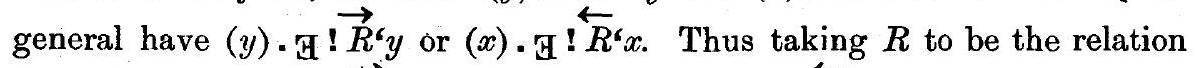
\includegraphics[max width=\textwidth, alt={}]{bc1848bf-39e8-4760-b069-9936044df683-117_68_1197_647_126} of parent and child, $\vec{R}^{c} y=$ the parents of $y$ and $\overleftarrow{R}^{c} x=$ the children of $x$. Thus $\overleftarrow{R}^{\prime} x=\Lambda$, i.e $\sim \nexists!\overleftarrow{R}^{\prime} x$, when $x$ is childless, and $\vec{R}^{\prime} y=\Lambda$, i.e. $\sim H^{\prime}!\vec{R}^{\prime} y$, when $y$ is Adam or Eve. The two sorts of existence, $\mathrm{E}!\vec{R}^{\prime} y$ and $y!\vec{R}^{\prime} y$, can both be significantly predicated of $\vec{R}^{\prime} y$, because " $\overrightarrow{R^{\prime}} y$ " is a descriptive function whose value is a class; and the same applies to $\overleftarrow{R^{\prime}} x$. It will be seen that (by $* 14 \cdot 21$ ) $\mathcal{H}!\vec{R}^{\prime} y .2 . \mathrm{E}!\vec{R}^{\prime} y$, but the converse implication does not hold in general.

We have\\
*32:16. $\vdash: \vec{R}=\vec{S} \cdot \equiv \cdot \overleftarrow{R}=\overleftarrow{S} \cdot \equiv \cdot R=S$\\
Aso by $* 32 \cdot 18 \cdot 181$,

$$
\vdash: x \in \vec{R}^{\prime} y . \equiv . x R y . \equiv . y \in \overleftarrow{R^{\prime}} x
$$

Thus by the use of $\vec{R}^{\prime} y$ or $\overleftarrow{R}^{\prime} x$, every statement of the form " $x R y$ " can be reduced to a statement asserting membership of a class. Since, however, the class in question is given by a descriptive function, and descriptive functions are defined by means of relations, we do not thus obtain a method of reducing the theory of relations to the theory of classes.\\
*32.01. $\vec{R}=\hat{a} \hat{y}\{\alpha=\hat{x}(x R y)\} \quad$ Df\\
*32.02. $\overleftarrow{R}=\hat{\beta} \hat{x}\{\beta=\hat{y}(x R y)\} \quad$ Df\\
*32.03. $\mathrm{sg}=\hat{A} \hat{R}(A=\vec{R}) \mathrm{Df}$\\
*3204. $\mathrm{gs}=\hat{A} \hat{R}(A=\overleftarrow{R}) \mathrm{Df}$\\
*32.1. $\mathrm{F}: \alpha \vec{R} y . \equiv \alpha=\hat{x}(x R y)[* 21 \cdot 3 .(* 32 \cdot 01)]$\\
*32:101. $\mathrm{F}: \beta \overleftarrow{R} x . \equiv . \beta=\hat{y}(x R y) \quad[* 21 \cdot 3 .(* 32 \cdot 02)]$\\
*32:11. ト. $\hat{x}(x R y)=\vec{R}^{\prime} y$ [*32•1.*30:3]\\
$* 32 \cdot 111 .+. \hat{y}(x R y)=\overleftarrow{R^{\prime}} x \quad[* 32 \cdot 101 \cdot * 30 \cdot 3]$\\
*32.12. F. E! $\vec{R}^{\prime} y$ [*32.11.*14.21]\\
*32:121. V. $\mathrm{E}!\stackrel{\leftarrow}{R}^{\prime} x \quad$ [*32.111.*14:21]\\
" $\mathrm{E}!\vec{R}^{\prime} y$ " must not be confounded with " $\vec{H}!\vec{R}^{\prime} y$." The former means that there is such a class as $\vec{R}^{c} y$, which, as we have just seen, is always true; the latter means that $\vec{R}^{\prime} y$ is not null, which is only true if $y$ is a term to which some other term has the relation $R$. Note that, by $* 14 \cdot 21$, both $\mathrm{G}^{\prime}!\vec{R}^{\prime} y$ and $\sim$ H! $\overrightarrow{R^{c}} y$ imply $\mathrm{E}!\vec{R}^{c} y$. The contradictory of $\operatorname{H}^{\prime} \vec{R}^{c} y$ is not $\sim$ H! $\vec{R}^{c} y$, but $\sim\left\{\left[\vec{R}^{c} y\right] \cdot\left\{\vec{R}^{c} y\right\}\right.$. This last would not imply $\mathrm{E}!\vec{R}^{c} y$, but for the fact that $\mathrm{E}!\vec{R}^{\prime} y$ is always true.\\
*32.13. $\mathrm{F} . \vec{R}^{c} y=\widehat{x}(x R y)$ [*32.11.*20.59]\\
*32.131. $+. \overleftarrow{R^{\prime}} x=\hat{y}(x R y)$ [*32.111.*20.59]\\
*32:132. $\vdash: \alpha \vec{R} y . \equiv \alpha=\overrightarrow{R^{\prime}} y . \equiv \alpha=\hat{x}(x R y)[* 32 \cdot 1 \cdot 13 . * 20 \cdot 57]$\\
*32.133. $\mathrm{F}: ~ \stackrel{\leftarrow}{\beta} x . \equiv \beta=\overleftarrow{R}^{\prime} x . \equiv \beta=\hat{y}(x R y)$ [*32.101•131.*20.57]\\
The use of *20.57 will in general be tacit. It happens constantly that we have propositions such as $* 32 \cdot 13$, in which a descriptive expression is shown to be identical with a class. In such cases, whenever the properties of the class are asserted of the descriptive expression, $* 20.57$ is relevant.\\
*32.14. $\mathrm{F}: \vec{R}=\vec{S} . \equiv . R=S$\\
Dem.

$$
\begin{aligned}
& \text { + . *21.43. ว! : } \vec{R}=\vec{S} . \equiv: \alpha \vec{R} y . \equiv_{a, y} . \overrightarrow{\alpha S} y \text { :. } \\
& {[* 32 \cdot 1] \quad \equiv: \alpha=\hat{x}(x R y) \cdot \equiv_{\alpha, y} \cdot \alpha=\hat{x}(x S y): .} \\
& \text { [*11•2] } \quad \equiv: .(y): . \alpha=\widehat{x}(x R y) . \equiv_{\alpha} . \alpha=\widehat{x}(x S y): . \\
& \text { [*2025] } \equiv: .(y): \hat{x}(x R y)=\hat{x}(x S y): \text {. } \\
& \text { [*20-15] } \quad \equiv: .(y): .(x): x R y . \equiv . x S y: . \\
& \text { [*11•2] } \quad \equiv: .(x, y): x R y . \equiv . x S y: . \\
& \text { [*21•43] } \equiv: . R=S:: \text { つ } \text { ᄀ . Prop }
\end{aligned}
$$

*32.15. $\vdash: \overleftarrow{R}=\overleftarrow{S} . \equiv R=S$ [Similar proof]\\
*32.16. $\vdash: \vec{R}=\vec{S} . \equiv \overleftarrow{R}=\overleftarrow{S} . \equiv R=S \quad[* 32 \cdot 14 \cdot 15]$\\
*32.18. $+: x \in \overrightarrow{R^{\prime}} y . \equiv . x R y$ [*32.13.*20.33]\\
*32:181. $\vdash: y \in \overleftarrow{R^{\prime}} x . \equiv x R y$ [*32131.*20.33]\\
*32.182. $\mathrm{F}: x \in \vec{R}^{\prime} y . \equiv . y \in \overleftarrow{R^{\prime}} x \quad$ [*32.18.181]

The transformation from＂$x R y$＂to＂$x \in \overrightarrow{R^{\prime}} y$＂is one commonly effected in language．E．g．suppose＂$x R y$＂is＂$x$ loves $y$ ，＂then＂$x \in \overrightarrow{R^{\prime}} y$＂is＂$x$ is a lover of $y$ ．＂\\
＊3219．$+: R \in S$. J．$\vec{R}^{c} y \subset \vec{S}^{c} y, \overleftarrow{R}^{c} x \subset \overleftarrow{S}^{c} x$\\
Dem．


\begin{align*}
& \text { ト.*32.18. ɔ : . Hp. ɔ : } x \in \vec{R}^{\prime} y . \partial_{x}, x \in \vec{S}^{\prime} y \text { : } \\
& \text { [*22-1] } \quad \supset: \vec{R}^{\prime} y \subset \vec{S}^{\prime} y  \tag{1}\\
& \text { ト. *32-181. ɔト:. Hp. ɔ: } y \in \overleftarrow{R^{6}} x . \supset_{y} . y \in \overleftarrow{S^{6}} x \text { : } \\
& \text { [*22-1] つ: } \overleftarrow{R^{\prime}} x \subset \overleftarrow{S^{\prime}} x  \tag{2}\\
& \text { ト.(1).(2). ɔ } . \text { Prop }
\end{align*}


＊32．2．$\vdash: A$ sg $R . \equiv . A=\vec{R}[* 21.3 .(* 32.03)]$\\
＊32＊201．$\vdash: A \mathrm{gs} R . \equiv A=\overleftarrow{R}$［＊213．（＊32．04）］\\
＊32．21．$+. \vec{R}=\operatorname{sg}^{6} R$［＊32．2．＊30．3］\\
＊32＊211． $\mathrm{F} . \overleftarrow{R}=\mathrm{gs}^{6} R \quad[* 32 \cdot 201 . * 30 \cdot 3]$\\
＊32＊22． $\mathrm{F} . \mathrm{E}!\mathrm{sg}^{6} R$［＊32．21．＊14．21］\\
＊32＊221． $\mathrm{F} . \mathrm{E}!\mathrm{gs}^{\prime} R$［＊32211．＊14．21］\\
＊32＊23．$+. \operatorname{sg}^{\prime} R=\vec{R} \quad[* 32 \cdot 21 . * 21 \cdot 2 \cdot 57]$\\
＊32＊231． t．$^{\text {gs }}{ }^{\prime} R=\overleftarrow{R} \quad[* 32 \cdot 211 \cdot * 21 \cdot 2 \cdot 57]$\\
＊32＊24． ト $. \operatorname{sg}^{c} \breve{R}=\operatorname{gs}^{c} R$\\
Dem．

$$
\begin{array}{lll}
\vdash \cdot * 32 \cdot 23 \cdot(* 32 \cdot 01) \cdot & \supset \vdash \cdot \operatorname{sg}^{\prime} \breve{R}=\hat{a} \hat{y}\{\alpha & =\hat{x}(x \breve{R} y)\} \\
{[* 21 \cdot 33]} & \supset \vdash: \alpha\left(\operatorname{sg}^{\prime} \breve{R}\right) y & \equiv \alpha=\hat{x}(x \breve{R} y) \\
{[* 31 \cdot 11 \cdot * 20 \cdot 15]} & & \equiv \alpha=\hat{x}(y R x) \\
{[* 32 \cdot 101]} & & \equiv \alpha \overleftarrow{R} x \\
{[* 32 \cdot 211]} & & \equiv \alpha\left(\operatorname{gs}^{\prime} R\right) x \\
\vdash \cdot(1) \cdot * 11 \cdot 11 \cdot * 21 \cdot 43 . \supset \vdash . \text { Prop } &
\end{array}
$$

＊32＊241． l $_{\text {⋅ }}$ gs $^{6} \breve{R}=\operatorname{sg}^{6} R \quad$［Similar proof］\\
＊32＊25． $\mathrm{F}: A \operatorname{sg} R . \equiv A=\operatorname{sg}^{\prime} R \quad$［＊30．4．＊3222］\\
＊32．251． $\mathrm{t}: A \mathrm{gs} R . \equiv . A=\mathrm{gs}^{\prime} R$［＊30．4．＊32．221］\\
＊323．$\quad$＋$\left\{\operatorname{sg}^{6}(R \cap S)\right\}^{6} y=\vec{R}^{6} y \cap \vec{S}^{6} y$\\
Note that we do not have

$$
\operatorname{sg}^{\prime}(R \dot{\cap} S)=\operatorname{sg}^{\prime} R \dot{\cap} \operatorname{sg}^{\prime} S
$$

Dem．

$$
\begin{aligned}
\vdash \cdot * 32 \cdot 23 \cdot 13 . \supset+.\left\{\operatorname{sg}^{6}(R \dot{n} S)\right\}^{6} y & =\widehat{x}\{x(R \dot{\cap} S) y\} \\
& =\widehat{x}(x R y \cdot x S y) \\
{[* 23 \cdot 33] } & =\widehat{x}(x R y) \cap \widehat{x}(x S y) \\
{[* 22 \cdot 39] } & =\overrightarrow{R^{\prime}} y \cap \vec{S}^{6} y . \supset \vdash . \text { Prop } \\
{[* 32 \cdot 13] } & \leftarrow \quad \leftarrow \quad \leftarrow \quad
\end{aligned}
$$

＊32：31．$\quad$ ㅏ $\cdot\left\{\text { gs }^{6}(R \dot{\cap} S)\right\}^{6} x=\overleftarrow{R}^{6} x \cap \overleftarrow{S^{6}} x$\\
＊3232．$\quad$ ㅏ．$\left\{\operatorname{sg}^{6}(R \cup S)\right\}^{6} y=\vec{R}^{6} y \cup \overrightarrow{S \prime}^{6} y$\\
＊32＊33．$\quad$ ㅏ．$\left\{\mathrm{gs}^{6}(R \cup S)\right\}^{6} x=\overleftarrow{R^{6}} x \cup \overleftarrow{S^{6}} x$\\
＊3234．$+\cdot\left\{\operatorname{sg}^{\prime}(\dot{-} R)\right\}^{\prime} y=-\vec{R}^{\prime} y$\\
＊3235． ᄀ ⋅ $\left\{\mathrm{gs}^{\mathrm{c}}(-R)\right\}^{6} x=-\overleftarrow{R}^{6} x$\\
The proofs of the above propositions are similar to that of $* 32 \cdot 3$ ．\\
＊324．$+:$ E！$R^{\prime} z_{. \equiv}:$ H！$\vec{R}^{\prime} z: x, y \in \vec{R}^{\prime} z . \partial_{x, y} . x=y$［＊30．21．＊32．18］\\
＊3241．F：．E！$S^{c} y . \supset: \vec{R}^{c} y=\vec{S}^{c} y . \equiv R^{c} y=S^{c} y$\\
Dem．\\
ト．＊4：86．$\supset \vdash:: x S y . \equiv_{x} . x=b: \supset:$.


\begin{equation*}
x R y . \equiv_{x} . x S y: \equiv: x R y . \equiv_{x} . x=b \tag{1}
\end{equation*}


$\vdash .(1) . * 532$. つ $: . x S y . \equiv_{x} . x=b: x R y . \equiv_{x} . x S y: \equiv:$


\begin{equation*}
x S y \cdot \equiv_{x} \cdot x=b: x R y \cdot \equiv_{x}, x=b \tag{2}
\end{equation*}


ト．（2）．＊10•11•281．＊32•18•181．J\\
F：．（马b）$: x S y . \equiv_{x} . x=b: \vec{R}^{\prime} y=\vec{S}^{\prime} y: \equiv:($ I $b): x S y . \equiv_{x} . x=b: x R y . \equiv_{x} . x=b:$\\
［＊30：3．＊14•13］\\
$\equiv:\left(\mathcal{H}^{b}\right): x S y . \equiv_{x} . x=b: R^{6} y=b:$\\
［＊14＊101］


\begin{equation*}
\equiv: R^{6} y=S^{6} y \tag{3}
\end{equation*}


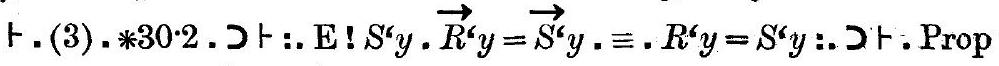
\includegraphics[max width=\textwidth, alt={}, center]{bc1848bf-39e8-4760-b069-9936044df683-120_66_999_1339_213}\\
＊32＊42．＋：$\vec{R}^{\prime} y=\vec{S}^{\prime} y . \supset: \mathrm{E}!R^{\prime} y . \equiv \mathrm{E}!S^{\prime} y \quad[* 30 \cdot 34 \cdot * 32 \cdot 18]$

\section*{*33. DOMAINS, CONVERSE DOMAINS, AND FIELDS OF RELATIONS}
\section*{Summary of *33.}
If $R$ is any relation, the domain of $R$, which we denote by $D^{\prime} R$, is the class of terms which have the relation $R$ to something or other; the converse domain, $\mathbb{I}^{\prime} R$, is the class of terms to which something or other has the relation $R$; and the field, $C^{6} R$, is the sum of the domain and the converse domain. (Note that the field is only significant when $R$ is a homogeneous relation.)

The above notations $\mathrm{D}^{c} R, \mathbb{C}^{c} R, C^{c} R$ are derivative from the notations $\mathrm{D}, \mathrm{G}, C$ for the relations, to a relation, of its domain, converse domain, and field respectively. We are to have

$$
\begin{aligned}
\mathrm{D}^{\prime} R & =\hat{x}\{(\mathrm{H} y) \cdot x R y\} \\
\mathrm{G}^{\prime} R & =\hat{y}\{(\mathrm{H} x) \cdot x R y\} \\
C^{\prime} R & =\hat{x}\{(\mathrm{H} y): x R y \cdot \mathrm{v} \cdot y R x\} ;
\end{aligned}
$$

hence we define $\mathrm{D}, \mathrm{G}, C$ as follows:\\
*33.01. $\mathrm{D}=\hat{a} \hat{R}[\alpha=\hat{x}\{($ H $y) . x R y\}] \quad$ Df\\
*33.02. $\mathrm{I}=\hat{\beta} \hat{R}[\beta=\hat{y}\{(\mathrm{G} x) . x R y\}] \quad$ Df\\
*33.03. $C=\hat{\gamma} \hat{R}[\gamma=\hat{x}\{($ H $y): x R y . \mathrm{v} . y R x\}] \quad$ Df\\
The letter $C$ is chosen as the initial of the word "campus." We require one other definition, namely of the relation of $x$ to $R$ when $x$ is a member of the field of $R$. This relation, which we will call $F$, is defined as follows:\\
*33.04.

$$
F=\hat{x} \hat{R}\{(\forall y): x R y . \mathrm{v} . y R x\} . \mathrm{Df}
$$

We shall find that $C=\vec{F} . \breve{\mathrm{D}}$ will be the relation of a relation to its domain, $\overleftarrow{D^{\prime}} \alpha$ will be the class of relations having $\alpha$ for their domain. Simitar remarks apply to $\mathbb{I}$ and $C$. The field of a relation is specially important in connection with series.

The propositions of this number are constantly used throughout the remainder of the work. The ideas of the domain, converse domain, and field are very general, and have somewhat different uses for relations of different kinds. Consider first the sort of relation that gives rise to a descriptive function $R^{6} y$. For this we require that $R^{6} y$ should exist whenever there is anything having the relation $R$ to $y$, i.e. that there should never be more than one term having the relation $R$ to a given term $y$. In this case, the values of $y$ for which $R^{\prime} y$ exists will constitute the "converse domain" of $R$, i.e. $I^{\prime} R$, and the values which $R^{\prime} y$ assumes for various values of $y$ will\\
constitute the "domain" of $R$, i.e. $\mathrm{D}^{\prime} R$. Thus the converse domain is the class of possible arguments for the descriptive function $R^{\prime} y$, and the domain is the class of all values of the function. Thus, for example, if $R$ is the relation of the square of an integer $y$ to $y$, then $R^{6} y=$ the square of $y$, provided $y$ is an integer. In this case, $\mathbb{C}^{\prime} R$ is the class of integers, and $D^{\prime} R$ is the class of perfect squares. Or again, suppose $R$ is the relation of wife to husband; then $R^{\prime} y=$ the wife of $y, \mathbb{C}^{\prime} R=$ married men, $\mathrm{D}^{\prime} R=$ married women. In such cases, the field usually has little importance; and if the values of the function $R^{6} y$ are not of the same type as its arguments, i.e. if the relation $R$ is not komogeneous, the field is meaningless. Thus, for example, if ⋅ $R$ is a homogeneous relation, $\vec{R}$ and $\overleftarrow{R}$ are not homogeneous, and therefore " $C \quad \vec{R}$ " and " $C \quad \overleftarrow{R}$ " are meaningless.

Let us next suppose that $R$ is the sort of relation that generates a series, say the relation of less to greater among integers. Then $\mathrm{D}^{\prime} R=$ all integers that are less than some other integer $=$ all integers, $\mathbb{I}^{\prime} R=$ all integers that are greater than some other integer $=$ all integers except 0 . In this case, $C^{6} R=$ all integers that are either greater or less than some other integer = all integers. Generally, if $R$ generates a series, $\mathrm{D}^{\wedge} R=$ all members of the series except the last (if any), $\mathbb{G}^{\prime} R=$ all members of the series except the first (if any), and $C^{6} R=$ all members of the series. In this case, " $x F R$ " expresses the fact that $x$ is a member of the series. Thus when $R$ generates a series, $C^{\prime} R$ becomes important, and the relation $F$ is likely to be useful.

We shall have occasion to deal with many relations having some of the properties of series, and with many propositions which, though only important in connection with serial relations, hold much more generally. In such cases, the field of a relation is likely to be important. Thus in the section on Induction (Part II, Section E), where we are preparing the way for the construction of serial relations by means of a certain kind of non-serial relation, and throughout relation-arithmetic (Part IV), the fields of relations will occur constantly. But in the earlier parts of the work, it is chiefly domains and converse domains that occur.

Among the more important properties of domains, converse domains and fields, which are proved in the present number, are the following.

We have always $\mathrm{E}!\mathrm{D}^{6} R, \mathrm{E}!\Phi^{6} R, \mathrm{E}!C^{6} R(* 33 \cdot 12 \cdot 121 \cdot 122)$. (The last of these, however, is only significant when $R$ is homogeneous.)\\
*33.13. $\vdash: x \in \mathrm{D}^{\prime} R . \equiv$. ( $\mathrm{H} y$ ). $x R y$\\
*33.131. $\vdash: y \in \mathbb{C}^{\prime} R . \equiv .\left(\mathbb{H}^{x}\right) . x R y$\\
*33132. $\vdash: . x \epsilon C^{6} R . \equiv:($ H $y): x R y$. v . $y R x$\\
*33.14. $\quad \vdash: x R y$. J $. x \in \mathrm{D}^{6} R . y \in \mathrm{~T}^{6} R$\\
*33:16. ㅏ. $C^{6} R=\mathrm{D}^{6} R \cup \mathbb{G}^{6} R$\\
＊33．2．21．22．The converse domain of a relation is the domain of its converse， the domain of a relation is the converse domain of its converse，and the field of a relation is the field of its converse．\\
＊3324． $\mathrm{F}: \mathrm{H}!\mathrm{D}^{\wedge} R . \equiv$ ．H！C‘ $R . \equiv$ ．H！$C^{\wedge} R . \equiv$ ．H！$R$\\
＊33．4．＋．D＇R＝$\hat{x}\left\{\right.$ H！$\left.\overleftarrow{R}^{\prime} x\right\}$\\
with corresponding propositions（ $\boldsymbol{*} \mathbf{3 3} \cdot \mathbf{4 1} \cdot \mathbf{4 2}$ ）for $\mathbb{C}^{\prime} R$ and $C^{\prime} R$ ．\\
＊33＊43．F ：E ！R ${ }^{6} y$. J $. y \in \mathbb{G}^{6} R . R^{6} y \in \mathrm{D}^{6} R$\\
＊33＊431． $\mathrm{F}:(y) . \mathrm{E}!R^{6} y . \supset .(\beta) . \beta \subset \mathrm{C}^{6} R$\\
＊33．5．＋．$C=\vec{F}$\\
＊33 51 ．F：$x \in C^{6} R . \equiv . x F R$\\
The proofs of propositions concerning $G$ and $C$ are usually similar to those for D，and are therefore often omitted．\\
＊33．01． $\mathrm{D}=\hat{a} \hat{R}[\alpha=\hat{x}\{($ H $y) \cdot x R y\}] \quad \mathrm{Df}$\\
＊33．02． $\mathrm{I}=\hat{\beta} \hat{R}[\beta=\hat{y}\{(, H x) . x R y\}] \quad$ Df\\
＊33．03．$C=\hat{\gamma} \hat{R}[\gamma=\hat{x}\{($ H $y): x R y \cdot \mathrm{v} \cdot y R x\}] \quad$ Df\\
＊33．04．$F=\hat{x} \hat{R}\{($ H $y): x R y . \mathrm{v} . y R x\} \quad$ Df\\
＊331． $\mathrm{F}: \alpha \mathrm{DR} . \equiv \alpha=\widehat{x}\{(\mathrm{y} y) . x R y\} \quad$［＊213．（＊33．01）］\\
＊33：101． $\mathrm{F}: \beta \mathrm{G} R . \equiv \beta=\widehat{y}\left\{\left(\mathrm{H}^{x}\right) . x R y\right\}$\\
＊33•102． $\mathrm{F}: \gamma C R . \equiv . \gamma=\widehat{x}\{($ H $y): x R y . \mathrm{v} . y R x\}$\\
＊33．103． $\mathrm{F}:, x F R . \equiv:(\mathrm{H} y): x R y . \mathrm{v} . y R x$\\
＊33．11．F． $\mathrm{D}^{6} R=\widehat{x}\{(\mathrm{H} y) . x R y\} \quad[* 33.1 . * 30.3 . * 20.59]$\\
＊33＇111．ト． $\mathrm{I}^{\top} R=\hat{y}\left\{\left(\mathrm{H}^{x}\right) \cdot x R y\right\}$\\
＊33•112．＋．$C^{\prime} R=\widehat{x}\{($ H $y): x R y$ ．v ．$y R x\}$\\
＊33：12．ト．E！D＇$R$［＊33．11．＊14•21］\\
＊33＇121． ト E ！ $\mathrm{G}^{\prime} R$\\
＊33 122．＋．E！$C^{6} R$\\
＊33．123． $\mathrm{F}: \alpha \mathrm{D} R . \equiv \alpha=\mathrm{D}^{\prime} R \quad[* 30.4 . * 33.12]$\\
＊33．124． $\mathrm{F}: \beta \mathrm{G} R . \equiv \beta=\mathrm{G}^{\prime} R$［＊30．4．＊33．121］\\
＊33．125． $\mathrm{F}: \gamma C R . \equiv \gamma=C^{6} R \quad$［＊30．4．＊32．123］\\
＊33．13．$F: x \in \mathrm{D}^{6} R . \equiv$ ．（마 $y$ ）．$x R y$［＊33．11．＊20．357］\\
＊33•131．$\vdash: y \in \mathbb{C}$ ⋅ $R$ ．三 ．$(\mathbb{H} x)$ ．$x R y$\\
＊33 132．F：$x \in C^{6} R . \equiv:($ H $y): x R y . \mathrm{v}, y R x$\\
＊33•14．$\vdash: x R y$ ．$\supset . x \in \mathrm{D}^{\circ} R . y \in \mathbb{G}^{\circ} R$\\
Dem．

$$
\begin{aligned}
& \vdash \cdot * 10 \cdot 24 . \text { つト: Hp. } \text { ɔ }:(\text { H } y) \cdot x R y:\left(\mathrm{H}^{x}\right) \cdot x R y: \\
& {[* 33 \cdot 13 \cdot 131] \quad \text { J }: x \in \mathrm{D}^{\prime} R \cdot y \in \mathbb{Q}^{\prime} R: \text { J } \text {. Prop }}
\end{aligned}
$$

＊33．15．$\quad$ ト.$\vec{R}^{\prime} y \in D^{\prime} R$\\
Dem．

$$
\begin{array}{ll}
\vdash \cdot * 32 \cdot 18 \cdot \supset \vdash: x \in \vec{R}^{6} y \cdot \partial_{x} \cdot x R y . \\
{[* 10 \cdot 24]} & \partial_{x} \cdot(\text { H } y) \cdot x R y . \\
{[* 33 \cdot 13]} & \partial_{x} \cdot x \in \mathrm{D}^{6} R: \supset \vdash . \text { Prop }
\end{array}
$$

＊33 151．ト．$\overleftarrow{R}^{\prime} x \subset G^{\prime} R$\\
＊33－152． ト $\cdot \vec{R}^{c} x \cup \overleftarrow{R}^{c} x \subset C^{c} R$\\
＊33•16． F．$C^{6} R=\mathrm{D}^{6} R \cup \mathbb{G}^{6} R$\\
Dem．


\begin{align*}
& \text { ト.*33.132.*1042.つ } \\
& \text { । : } x \in C^{6} R . \equiv:(\text { gy }) . x R y . \mathrm{v} .(\text { H } y) . y R x: \\
& {[* 33 \cdot 13 \cdot 131] \equiv: x \in \mathrm{D}^{\prime} R . \vee \wedge x \in \mathbb{C}^{\prime} R:} \\
& {[* 22 \cdot 34] \quad \equiv: x \in \mathrm{D}^{\prime} R \cup \mathbb{C}^{\prime} R}  \tag{1}\\
& \text { ト.(1).*10.11.*20.43. } . \text { つ } \text {. Prop }
\end{align*}


＊33．161．＋． $\mathrm{D}^{4} R \subset C^{6} R . \mathrm{G}^{4} R \subset C^{6} R \quad[* 33 \cdot 16 . * 22 \cdot 58]$\\
＊3317．$F: x R y$. J $. x, y \in C^{6} R$［＊3314－161］\\
＊3318．$\leqslant: \mathrm{D}^{c} R=\mathrm{G}^{c} R$ ．$\supset . \mathrm{D}^{c} R=C^{c} R$\\
Dem．

$$
\begin{array}{rlrl}
\vdash \cdot * 22 \cdot 56 . & \supset \vdash: \mathrm{D}^{\wedge} R=\mathbb{C}^{\wedge} R . & \supset . \mathrm{D}^{\wedge} R & =\mathrm{D}^{\wedge} R \cup \mathbb{G}^{\wedge} R \\
& =C^{\wedge} R: \supset \vdash . \text { Prop } \\
{[* 33 \cdot 16]} &
\end{array}
$$

＊33－181．$+: \mathbb{C}^{6} R \subset \mathrm{D}^{6} R . \equiv \mathrm{D}^{6} R=C^{6} R$\\
Dem．

$$
\begin{aligned}
& \vdash \cdot * 22 \cdot 62 . \supset \vdash: \mathbb{C}^{\prime} R \subset \mathbb{D}^{\prime} R . \equiv \mathrm{D}^{\prime} R=\mathrm{D}^{\prime} R \cup \mathbb{C}^{\prime} R \\
& =C^{\kappa} R: \supset \vdash . \text { Prop } \\
& \begin{array}{ll}
{[* 33 \cdot 16]} & \\
\vdash: \mathrm{D}^{\prime} R \subset \mathbb{C}^{\prime} R . \equiv . \mathbb{C}^{\prime} R=C^{\prime} R \quad[\text { imilar proof }]
\end{array}
\end{aligned}
$$

If $R$ is the sort of relation which generates a series，so that＂$x R y$＂may be read＂$x$ precedes $y$ ，＂then $\mathcal{G}^{\prime} R \subset D^{\prime} R$ is the condition that the series may have no last term，since it states that every term which follows some term precedes some other term，and is therefore not the last of the series．\\
＊33．2．

$$
\vdash . G^{\prime} R=D^{s} \breve{R}
$$

Dem．


\begin{align*}
& \vdash . * 31 \cdot 11 . * 10 \cdot 11 . \supset \vdash: x R y . \equiv_{x} . y \breve{R} x: \\
& {[* 10 \cdot 281] \quad \supset \vdash:(\mathbb{H} x) . x R y . \equiv .(\mathrm{H} x) . y \breve{R} x:} \\
& {[* 33 \cdot 13 \cdot 131] \quad \supset \vdash: y \in \mathbb{G}^{\prime} R . \equiv y \in \mathrm{D}^{\prime} R}  \tag{1}\\
& \vdash .(1) . * 10 \cdot 11 \cdot * 20 \cdot 43 . \text { J } . \text { Prop }
\end{align*}


＊3321．F． $\mathrm{D}{ }^{\prime} \boldsymbol{R}=\mathrm{G} \bullet \breve{R} \quad$［Similar proof］\\
＊33．22．$\quad$ ト．$C^{6} R=C^{6} \breve{R}$\\
Dem．

$$
\begin{aligned}
\vdash \cdot * 33 \cdot 16 \cdot 2 \cdot 21 . \supset \vdash . C^{6} R & =G^{6} \breve{R} \cup D^{6} \breve{R} \\
{[* 33 \cdot 16] } & =C^{6} \breve{R} . \supset \vdash . \text { Prop }
\end{aligned}
$$

＊33．24．$F: G!D^{c} R . \equiv$ H！ $\mathbb{C}^{c} R . \equiv$ H！$C^{c} R . \equiv$ H！$R$\\
Dem．


\begin{align*}
& \text { [*25.5.(*11.03)] } \quad \equiv: \text { 守! } R  \tag{1}\\
& \text { ト.*33131. ɔ }=\mathcal{H}^{\prime} \mathcal{U}^{\prime} R \equiv:(H y):(H x) . x R y: \\
& \text { [*11:2] } \equiv:(\mathrm{H} x, y) . x R y \text { : } \\
& \text { [*25:5] } \equiv \div \mathbf{I}!R  \tag{2}\\
& \text { ト.*33-132. ว!: } A!C^{6} R \equiv:\left(H^{x}\right):(H y): x R y . v . y R x: . \\
& \text { [米117] } \quad \equiv \div(\mathrm{G} x, y) . x R y \text { : } \\
& \text { [*25.5] } \equiv \text { ± . I'R }  \tag{3}\\
& \text { ト..(1).(2). (3). } 2+\text {.Prop }
\end{align*}


＊33．241．$\leqslant \mathrm{D}^{\prime} R=\Lambda . \equiv \mathrm{C}^{\prime} R=\Lambda . \equiv C^{\prime} R=\Lambda . \equiv R=\dot{\Lambda}$\\
［＊33．24．Transp．＊24：51．＊25．51］\\
＊33．25．F． $\mathrm{D}^{6}(\boldsymbol{R} \cap S) \in \mathrm{D}^{6} \boldsymbol{R} \cap \mathrm{D}^{6} S$\\
Dem．

\[
\begin{array}{ll}
\vdash \cdot * 33 \cdot 13 . \text { Jr: } x \in \mathrm{D}^{\circ}(R \dot{A} S) \cdot \equiv:(\mathrm{H} y) \cdot x(R \dot{n} S) y: \\
{[* 21 \cdot 33 . * 10 \cdot 281]} & \equiv:(\mathrm{H} y) \cdot x R y \cdot x S y: \\
{[* 10 \cdot 5]} & \partial:(\mathrm{H} y) \cdot x R y:(\mathrm{H} y) \cdot x S y: \\
{[* 33 \cdot 13]} & \partial: x \in \mathrm{D}^{\prime} R \cdot x \in \mathrm{D}^{\prime} S: \\
{[* 21 \cdot 33]} & \partial: x \in \mathrm{D}^{\prime} R \cap \mathrm{D}^{\prime} S  \tag{1}\\
\text { F.(1).*10'11. JF.Prop } &
\end{array}
\]

＊33．251．F．$G^{6}(R \cap S) \subset G^{6} R \cap G^{6} S$［Similar proof］\\
＊33．252．F．$C^{6}(R \cap S) \subset C^{6} R \cap C^{6} S$［Similar proof］\\
＊3326．$\quad$ ㄱ． $\mathrm{D}^{4}(R \cup S)=\mathrm{D}^{6} R \cup \mathrm{D}^{4} S$\\
Dem．


\begin{align*}
& \text { [*23:34.*10:281] } \equiv:(\mathrm{H} y): x R y . v . x S y \text { : } \\
& \text { [*1042] } \equiv:(\text { সy }) . x R y: v:(\text { H } y) . x S y \text { : } \\
& \text { [*33.13]: } \equiv: x \in \mathrm{D}^{4} \text { R.v. } x \in \mathrm{D}^{\prime} S \text { : } \\
& \text { [*22:34] } \equiv: x \in \mathrm{D}^{\circ} R \cup \mathrm{D}^{\prime} S  \tag{1}\\
& \text { ト.(1).*1011.*2043. . } 2 \text {. Prop }
\end{align*}


＊33：261．F． $\mathbb{G}^{4}(R \mho S)=G$ \textbackslash ＆$R$ G $S$［Similar proof］\\
＊33262．F．$C^{6}(R \cup S)=C^{6} R \cup C^{6} S^{5} \quad[* 33 \cdot 26 \cdot 26116]$\\
＊33＊263．$F: R C S . O . D^{\prime} R \subset D^{\prime} S$\\
Dem．

$$
\begin{array}{ll}
\vdash \cdot * 23 \cdot 1 . \supset f: \text { Hp } . & \supset: x R y . \partial_{x, y} * x S y: \\
{[* 10 \cdot 28 \cdot 27]} & \supset:(x):(\text { Hy }) \cdot x R y . \supset .(\text { Hy }) \cdot x S y: \\
{[* 33 \cdot 13]} & \supset:(x): x \in D^{\prime} R . \supset \cdot x \in D^{\prime} S: \\
{[* 23 \cdot 1]} & \supset: D^{\prime} R \subset D^{\prime} S: \supset F . \text { Prop }
\end{array}
$$

＊33264． $\mathrm{F}: R \in S$. J． G $^{\prime} R \subset$ G $^{\prime} S$［Similar proof］\\
＊33．265． $\mathrm{F}: R \in S$. J．$C^{6} R \subset C^{6} S$［＊33．263．264．16．＊22．72］\\
＊33．27．F．$C^{6} R=\mathrm{D}^{6}(R \mho \breve{R})$\\
Dem．

$$
\begin{aligned}
\vdash \cdot * 33 \cdot 16 \cdot 2 \cdot \supset \vdash \cdot C^{6} R & =\mathrm{D}^{\prime} R \cup \mathrm{D}^{\prime} \breve{R} \\
{[* 33 \cdot 26] } & =\mathrm{D}^{\prime}(R \cup \breve{R}) \cdot \supset \vdash . \text { Prop }
\end{aligned}
$$

＊33．271．$+C^{6} R=Q^{\prime}(R \cup \breve{R})$ ［Similar proof］\\
＊33．272．F． $\mathrm{D}^{\prime}(R \circlearrowleft \breve{R})=\mathbb{G}^{\prime}(R \circlearrowleft \breve{R})=C^{\prime}(R \circlearrowleft \breve{R})=C^{\prime} R \quad[* 33 \cdot 27 \cdot 271 \cdot 16]$\\
＊33．28． $\mathrm{F} . \mathrm{D}{ }^{\prime} \mathrm{V}=\mathrm{G}^{\prime} \mathrm{V}=C^{\prime} \mathrm{V}=\mathrm{V}$\\
Dem．

$$
\begin{aligned}
& \text { ト. *1025.*25-104. ɔト:. }(x):(\text { H } y) . x \text { V } y: .(x):(\text { H } y) . y \text { V } x: .
\end{aligned}
$$


\begin{align*}
& \text { [*24-14] } \quad \partial \vdash: \mathrm{D}^{6} \dot{\mathrm{~V}}=\mathrm{V} . \mathrm{G}^{\prime} \dot{\mathrm{V}}=\mathrm{V}  \tag{1}\\
& \text { [*33.16] } \quad \supset \vdash . C^{6} \mathrm{~V}=\mathrm{V} \cup \mathrm{~V} \\
& \text { [*22.56] =V }  \tag{2}\\
& \text { ト.(1).(2).ɔト.Prop }
\end{align*}


＊33．29．F． $\mathrm{D}^{\prime} \dot{\Lambda}=\mathrm{G}^{\prime} \dot{\Lambda}=C^{\prime} \dot{\Lambda}=\Lambda \quad[* 33 \cdot 241 \cdot * 21 \cdot 2]$\\
＊33．3．$\quad$－：$\alpha \subset \mathrm{D}^{\prime} R . \equiv: x \in \alpha . \partial_{x} \cdot$ H！$R^{\prime} x$\\
Dem．

$$
\begin{aligned}
\vdash \cdot * 32 \cdot 181 \cdot \supset \vdash: x \in \alpha \cdot \partial_{x} \cdot \mathrm{H}^{1}!\overleftarrow{R}^{6} x: & \equiv: x \in \alpha \cdot \partial_{x} \cdot(\text { H } y) \cdot x R y: \\
{[* 33 \cdot 13] } & \equiv: x \in \alpha \cdot \partial_{x} \cdot x \in \mathrm{D}^{6} R: \text {. } \supset \vdash . \text { Prop }
\end{aligned}
$$

＊33．31．F：$\beta \subset \mathbb{C}^{\wedge} R . \equiv: y \in \beta . \supset_{y} \cdot \mathbb{H}^{\prime}!\vec{R}^{\prime} y \quad$［Proof as in＊333］\\
The three following propositions are used in the theory of selections（＊80， ＊83 and＊85）．The second of them is also used in the theory of greater and less（＊117）and in the theory of transitive relations（＊201）．\\
＊33．32．

$$
\mathrm{F}: \mathrm{D}^{\prime} R \cap \mathrm{D}^{\prime} S=\Lambda . \supset . R \dot{\circ} S=\dot{\Lambda}
$$

The converse of this proposition is not true．\\
Dem．

$$
\begin{aligned}
\forall \cdot * 23 \cdot 33 . & \supset \vdash: x(R \cap S) y \cdot \\
{[* 33 \cdot 14 \cdot * 22 \cdot 33] } & \\
& \supset \cdot x R y \cdot x S y . \\
& =D^{\top} R \cap D^{\top} S .
\end{aligned}
$$


\begin{align*}
& \text { [*10.24] } \quad J . \text { H }^{\prime} R \cap D^{\prime} S  \tag{1}\\
& \text { F.(1). Transp. ɔ : } \mathrm{D}^{\prime} R \cap \mathrm{D}^{\prime} S=\Lambda . \supset \cdots\{x(R \cap S) y\}  \tag{2}\\
& \text { ト. (2) . *11-113. } 2 \text { : : } \mathrm{D}^{\prime} R \cap \mathrm{D}^{\prime} S=\Lambda . \supset .(x, y) . \sim\{x(R \dot{n} S) y\} . \\
& \text { [*25.15] ɔ. } R \text { ก } S=\Lambda: \supset \vdash \text {. Prop }
\end{align*}


＊33．33．F： $\mathbb{G}^{\prime} R \cap \mathbb{G}^{\prime} S=\Lambda$. J．$R \dot{\circ} S=\dot{\Lambda} \quad$［Proof as in＊33．32］\\
＊33．34．F：$C^{6} R \cap C^{6} S=\Lambda . \supset . R \cap \dot{S}=\dot{\Lambda}$\\
Dem．

$$
\begin{aligned}
& \text { ト. *33•161.*2249. ɔㅇ. } \mathrm{D}^{6} R \cap \mathrm{D}^{6} S \subset C^{6} R \cap C^{6} S \text {. } \\
& \text { [*24-13] ɔ } \quad \text { J : } C^{6} R \cap C^{6} S=\Lambda . \supset . \mathrm{D}^{6} R \cap \mathrm{D}^{6} S=\Lambda \text {. } \\
& \text { [*33.32] ɔ.Ris=A:ว! Prop }
\end{aligned}
$$

＊33．35．$\vdash: . \mathrm{D}^{\wedge} R \mathrm{C} \alpha . \equiv: x R y . \supset_{x, y} . x \in \alpha$\\
Dem．

$$
\begin{aligned}
\vdash . * 33 \cdot 13 . \supset \vdash: \mathrm{D}^{\prime} R \subset \alpha . & \equiv:(\mathrm{H} y) . x R y . \partial_{x} . x \in \alpha: \\
{[* 10 \cdot 23] } & \equiv: x R y . \partial_{x, y} . x \in \alpha: . \supset \text {. Prop }
\end{aligned}
$$

＊33．351．$+: . \mathrm{C}^{6} R \subset \alpha . \equiv: x R y . \partial_{x, y}, y \in \alpha \quad$［Proof as in＊33．35］\\
＊33．352． $\mathrm{F}: . C^{4} R \mathrm{C} \alpha . \equiv: x R y . J_{x, y} . x, y \in \alpha$\\
Dem．

$$
\begin{aligned}
& \text { ト. } * 33 \cdot 16 \cdot * 22 \cdot 59 \cdot \supset \\
& \text { F:. } C^{6} R C \alpha \cdot \equiv: \mathrm{D}^{6} R \subset \alpha \cdot \mathrm{G}^{6} R \subset \alpha: \\
& {[* 33 \cdot 35 \cdot 351] \equiv: x R y \cdot J_{x, y} \cdot x \in \alpha: x R y \cdot J_{x, y} \cdot y \in \alpha:} \\
& {[* 11 \cdot 391] \quad \equiv: x R y \cdot J_{x, y} \cdot x, y \in \alpha: . \text { J F. Prop }}
\end{aligned}
$$

The two following propositions（＊33•441）are very frequently used．\\
＊33．4．$\quad$ ㅏ． $\mathrm{D}^{\prime} R=\widehat{x}\left\{\frac{H}{R^{\prime}} x\right\}$\\
Dem．


\begin{align*}
& \vdash \cdot * 33 \cdot 13 . \supset \vdash: x \in \mathrm{D}^{6} R . \equiv(\text { H } y) \cdot x R y . \\
& \text { [*32.181] } \quad \equiv .(\text { H } y) \cdot y \in \overleftarrow{R^{6}} x . \\
& \begin{aligned}
& {[* 24 \cdot 5] } \equiv \cdot \text { H! } \overleftarrow{R^{6}} x \\
& \vdash .(1) \cdot * 10 \cdot 11 \cdot * 20 \cdot 33 . \supset \vdash . \text { Prop }
\end{aligned} \tag{1}
\end{align*}


＊33－41．F． $\mathrm{G}^{\prime} R=\hat{y}\left\{\mathbb{H}!\vec{R}^{\prime} y\right\} \quad$［Similar proof］\\
＊33．42． ＋．$C^{6} R=\widehat{x}\left\{\right.$ 月！$\left.\left(\vec{R}^{6} x \cup \overleftarrow{R}^{6} x\right)\right\}$\\
Dem．

$$
\begin{aligned}
\vdash \cdot * 33 \cdot 4 \cdot 41 \cdot 16 . \supset+. C^{6} R & =\hat{x}\left\{G!\overrightarrow{R^{6}} x\right\} \cup \hat{x}\left\{G!\overleftarrow{R^{6}} x\right\} \\
{[* 22 \cdot 391] } & =\hat{x}\left\{G!\overrightarrow{R^{6}} x \cdot \mathrm{v} \cdot \mathrm{H}^{\prime}!\overleftarrow{R^{6}} x\right\} \\
{[* 24 \cdot 56 \cdot * 20 \cdot 15] } & =\hat{x}\left\{G!\left(\overrightarrow{R^{6}} x \cup \overleftarrow{R^{6}} x\right)\right\} \cdot \supset+. \text { Prop }
\end{aligned}
$$

＊3343．$+: \mathrm{E}!R^{6} y$. J $. y \in \mathrm{G}^{6} R . R^{6} y \in \mathrm{D}^{6} R$\\
Dem．

$$
\begin{aligned}
& \text { ト.*30.32. ɔ́ : E! Rsy. J. }\left(R^{6} y\right) R y \text {. } \\
& \text { [*33.14] J. } y \in \mathrm{G}^{\prime} R . R^{\prime} y \in \mathrm{D}^{\prime} R: \partial \dagger \text {. Prop }
\end{aligned}
$$

＊33．431． $.1(y) . E!R^{\prime} y$. J．$(\beta) . \beta \subset$ T $^{\prime} R$\\
Dem．\\
ト．＊33．43．$\quad \supset \mathrm{F}: \mathrm{Hp}: \supset: y \in \mathbb{G} \checkmark R$.


\begin{align*}
& {[\operatorname{Simp}] \quad \supset: y \in \beta . \supset . y \in \mathbb{G} R}  \tag{1}\\
& \vdash .(1) \cdot * 10 \cdot 11 \cdot 21 . \supset \vdash: \text { Hp } . \supset . \beta \subset G^{\prime} R  \tag{2}\\
& \vdash .(2) \cdot * 10 \cdot 11 \cdot 21 . \supset \vdash . \text { Prop }
\end{align*}


＊33．432． $\mathrm{F}:(y) . \mathrm{E}!R^{\prime} y .3 . \mathrm{I}^{\prime} R=\mathrm{V}$\\
Dem．

$$
\begin{aligned}
& \vdash \cdot * 33 \cdot 43 \cdot * 10 \cdot 11 \cdot 27 \cdot \supset \vdash: \mathrm{Hp} \cdot \supset \cdot(y) \cdot y \in \mathbb{G}^{6} R \\
& {[* 24 \cdot 14] \quad \text { つ. } \mathbb{G}^{\prime} R=\nabla: \supset \vdash . \text { Prop }}
\end{aligned}
$$

＊33：44．$\leqslant: \mathrm{E}!\breve{R}^{6} x$. J $. x \in \mathrm{D}^{6} R . \breve{R}^{6} x \in \mathbb{G} \boldsymbol{R}$\\
Dem．

$$
\begin{aligned}
& \vdash \cdot * 33 \cdot 43 \frac{\breve{R}}{R} \cdot \supset \vdash: \mathrm{Hp} \cdot \supset \cdot x \in \mathbb{G}^{6} \breve{R} \cdot \breve{R}^{6} x \in \mathrm{D}^{6} \breve{R} . \\
& {[* 33 \cdot 2 \cdot 21] \quad \supset \cdot x \in \mathrm{D}^{6} R \cdot \stackrel{\breve{R}}{R}^{6} x \in \mathbb{G}^{6} R: \supset \vdash . \text { Prop }}
\end{aligned}
$$

＊33．45． 上：$y \in \mathbb{C}^{6} R \cup \mathbb{C}^{6} S . \nu_{y} . R^{6} y=S^{6} y: \supset . R=S$\\
Note that by our conventions as to denoting expressions，the scope of both $R^{6} y$ and $S^{6} y$ in the above is＂$R^{6} y=S^{6} y$ ，＂and $R^{6} y$ is to be first eliminated．

Dem．


\begin{align*}
& \text { ト. } * 30 \text { 11. } \text { つt }:: R^{\prime} y=S^{\prime} y . \equiv:\left(\text { H }^{b}\right): x R y . \equiv_{x} . x=b: b=S^{\prime} \bar{y}: . \\
& \text { [*30-11] } \equiv:(\vec{G} b): x R y . \equiv_{x} . x=b: \text { (Gc) }: x: S y . \equiv_{x} . x=c: b=c: \\
& \text { [*13.195] } \equiv:\left(\text { g }^{b}\right): x R y . \equiv_{x} . x=b: x S y . \equiv_{x} \cdot x=b: . \\
& \text { [*10322] } \quad \text { : } x R y . \equiv_{x} . x S y  \tag{1}\\
& \text { ト.(1). ɔ }:: \mathrm{Hp} \text {. ɔ:. } y \in \mathbb{G}^{\prime} R \cup \mathbb{G}^{\prime} S . \supset: x R y . \equiv . x S y: . \\
& \text { [*532] } \quad \text { : } y \in \mathbb{G} \cdot R \cup \mathbb{G} \cdot S . x R y . \equiv y \in \mathbb{G} \cdot R \cup \mathbb{G} S . x S y: \\
& \text { [*33.14.*4.71] J:.xRy.三.xSy }  \tag{2}\\
& \text { ト.(2).*11113. ɔㄴ:. Hp. } \text { ɔ: }(x, y): x R y . \equiv . x S y \text { : } \\
& \text { [*2143] } \supset: R=S: . \supset f \text {. Prop } \\
& \text { *33.46. F: } x \in \mathrm{D}^{6} R \cup \mathrm{D}^{6} S . \partial_{x} . \breve{R}^{6} x=\breve{S}^{6} x: \supset . R=S \text { [Proof as in *33455] } \\
& \text { *33.47. } F: . y \in \mathbb{G}^{\prime} R \cup \mathbb{G}^{\prime} S . \partial_{y} . \vec{R}^{\prime} y=\vec{S}^{\prime} y: \supset . R=S
\end{align*}


Dem．


\begin{equation*}
\text { ト } \cdot * 33 \cdot 41 \text {. Transp } \cdot \supset \vdash: y \sim \epsilon \mathbb{G}^{\prime} R \cup \mathbb{G}^{\prime} S \cdot \supset \cdot \vec{R}^{\prime} y=\Lambda \cdot{\overrightarrow{S^{\prime}}}_{y}=\Lambda \tag{1}
\end{equation*}


$$
\begin{array}{ll}
\vdash \cdot(1) \cdot * 13 \cdot 172 \cdot * 4 \cdot 83 \cdot \supset \vdash: \mathrm{Hp} \cdot & \text { ɔ } \cdot(y) \cdot \overrightarrow{R^{\prime}} y=\overrightarrow{S^{\prime}} y \\
{[* 30 \cdot 41]} & \supset \cdot \vec{R}=\vec{S} \\
{[* 32 \cdot 14]} & \supset \cdot R=S: \supset \vdash . \text { Prop }
\end{array}
$$

*33.48. $+: . x \in \mathrm{D}^{\prime} R \cup \mathrm{D}^{\prime} S . \partial_{x} \cdot \overleftarrow{R^{\prime}} x=\overleftarrow{S^{\prime}} x: \supset . R=S \quad$ [Proof as in *33.47]\\
*33.5. ト. $C=\vec{F}$\\
Dem.


\begin{align*}
& \begin{aligned}
& \vdash \cdot * 32 \cdot 1.3 \vdash: \alpha \overrightarrow{F R} R . \equiv \alpha=\widehat{x}(x F R) \\
&=\widehat{x}\{(\mathrm{H} y): x R y . \mathrm{v} . y R x\} \\
& {[* 33 \cdot 103] } \equiv . \alpha C R \\
& {[* 33 \cdot 102] } \\
& \vdash .(1) \cdot * 11 \cdot 11 \cdot * 21 \cdot 43 . \supset+. \text { Prop }
\end{aligned}
\end{align*}


*33.51. $\vdash: x \in C C^{\prime} R . \equiv . x F R$ [*33.132•103]\\
$F$ is useful in ordinal arithmetic, where we are concerned with a series generated by a relation $P$, and " $x F P$ " expresses the fact that $x$ is a member of this series. The above two propositions ( $* 33551$ ) will be much used in Part IV, where we deal with the foundations of ordinal arithmetic, but will not often be referred to elsewhere.\\
*33.6. $\quad \vdash: R \in \overleftarrow{\mathrm{D}}^{\zeta} \alpha . \equiv \ldots=\mathrm{D}^{\kappa} R$\\
Dem.

$$
\begin{aligned}
\vdash . * 32 \cdot 181 . \supset \vdash: R \epsilon \overleftarrow{\mathrm{D}}^{\prime} \alpha . & \equiv . \alpha \mathrm{D} R . \\
{[* 33 \cdot 123] } & \equiv . \alpha=\mathrm{D}^{\prime} R: \supset \vdash . \text { Prop }
\end{aligned}
$$

*33.61. $\vdash: R \in \overleftarrow{\mathbb{T}}^{\prime} \alpha . \equiv . \alpha=\mathbb{G}^{\prime} R$\\
*33.62. $+: R \in \overleftarrow{C^{6}} \alpha . \equiv . \alpha=C^{6} R$

\section*{＊34．THE RELATIVE PRODUCT OF TWO RELATIONS}
Summary of＊34．\\
The relative product of two relations $R$ and $S$ is the relation which holds between $x$ and $z$ when there is an intermediate term $y$ such that $x$ has the relation $R$ to $y$ and $y$ has the relation $S$ to $z$ ．Thus e．g．the relative product of brother and father is paternal uncle；the relative product of father and father is paternal grandfather ；and so on．The relative product of $R$ and $S$ is denoted by＂$R \mid S$＂；the definition is ：\\
＊3401．$R \mid S=\hat{x} \hat{z}\{($ H $y) \cdot x R y \cdot y S \dot{z}\}$ Df\\
This definition is only significant when $C^{\prime} R$ and $D^{\prime} S$ belong to the same type．

The relative product of $R$ and $R$ is called the square of $R$ ；we put\\
＊34：02．$R^{2}=R \mid R \quad$ Df\\
＊34．03．$R^{3}=R^{2} \mid R$ Df\\
The most useful propositions in the present number are the following：\\
＊34－2．

$$
\vdash \cdot \operatorname{Cnv}^{\prime}(R \mid S)=\breve{S} \mid \breve{R}
$$

I．e．the converse of a relative product is obtained by turning each factor into its converse and reversing the order of the factors．\\
＊34．21．ト．$(P \mid Q)|R=P|(Q \mid R)$\\
I．e．the relative product obeys the associative law．\\
$* 3425$ ．$\quad$ ．$P \mid(Q \cup R)=(P \mid Q) \cup(P \mid R)$\\
＊34．26． ト．$(P \cup Q) \mid R=(P \mid R) \circlearrowleft(Q \mid R)$\\
I．e．the relative product obeys the distributive law with respect to the logical addition of relations．（For logical multiplication instead of logical addition，we only get inclusion instead of identity；cf． $\boldsymbol{*} \mathbf{3 4} \boldsymbol{2} \mathbf{2 3} \boldsymbol{\cdot} \mathbf{2 4}$ ．）\\
＊34．34．$\leqslant: R \subset P . S \subset Q$. J．$R|S \subset P| Q$\\
＊34：36． ト． $\mathrm{D}^{6}(P \mid Q) \subset \mathrm{D}^{6} P . \mathrm{G}^{6}(P \mid Q) \subset \mathrm{C}^{6} Q$\\
＊34．41． $\mathrm{F}: \mathrm{E}!P^{6} Q^{6} z \cdot$ J $\cdot P^{6} Q^{6} z=(P \mid Q)^{6} z$\\
＊3401．$R \mid S=\widehat{x} \widehat{z}\{($ H $y) . x R y . y S z\}$ Df\\
＊34：02．$R^{2}=R \mid R \quad$ Df\\
＊34．03．$R^{3}=R^{2} \mid R$ Df\\
＊34•1．$\vdash: x(R \mid S) z . \equiv$（Gy）．$x R y . y S z$［＊21•3．（＊34：01）］\\
＊34．11．$\vdash: x(R \mid S) z . \equiv \cdot \mathcal{H}!\left(\overleftarrow{R}^{6} x \cap \vec{S}^{6} z\right)$\\
Dem．

$$
\begin{aligned}
& \vdash \cdot * 34 \cdot 1 \cdot * 32 \cdot 18 \cdot 181 \cdot \supset \\
& \vdash: x(R \mid S) z \cdot \equiv \cdot(\mathrm{H} y) \cdot y \in \overleftarrow{R^{\prime}} x \cdot y \in \overrightarrow{S^{\prime}} z \cdot \\
& {[* 22 \cdot 33] \quad \equiv \cdot(\mathrm{H} y) \cdot y \in \overleftarrow{R^{\prime}} x \cap{\overrightarrow{S^{\prime}}}^{\prime} z .} \\
& {[* 24 \cdot 5] \quad \equiv \cdot \mathrm{H}!\left(\vec{R}^{\prime} x \cap \vec{S}^{\prime} z\right): \supset \text {. Prop }}
\end{aligned}
$$

＊34＇12．F．$R \mid S=\widehat{x} \widehat{z}\left\{\right.$ 固！$\left.\left(\overleftarrow{R^{\prime}} x \cap \vec{S}^{\prime} x\right)\right\} \quad[* 21 \cdot 33 . * 34 \cdot 11]$\\
＊342．$\quad$ ト． $\mathrm{Cnv}^{\prime}(R \mid S)=\breve{S} \mid \breve{R}$\\
Dem．

\[
\begin{array}{ll}
\vdash \cdot * 31 \cdot 131 \cdot \supset \vdash: x\left\{\operatorname{Cnv}^{c}(R \mid S)\right\} z & \equiv z(R \mid S) x . \\
{[* 34 \cdot 1]} & \equiv \cdot(\text { Hy }) \cdot z R y \cdot y S x . \\
{[* 31 \cdot 11]} & \equiv \cdot(\text { Hy }) \cdot y \breve{R} z \cdot x \breve{S} y . \\
{[* 34 \cdot 1]} & \equiv x(\breve{S} \mid \breve{R}) z  \tag{1}\\
\text { F. }(1) \cdot * 11 \cdot 11 \cdot * 21 \cdot 43 . \text { つト. Prop } &
\end{array}
\]

＊34：202． ト.$R\left|S=\left(\mathrm{Cnv}^{\prime} \breve{R}\right)\right| S$\\
Dem．


\begin{align*}
& \vdash \cdot * 31 \cdot 131 \cdot \supset \vdash: x\left(\mathrm{Cnv}^{6} \breve{R}\right) y \cdot y S z \cdot \equiv \cdot y \breve{R} x \cdot y S z \\
& \equiv x R y \cdot y S z  \tag{1}\\
& {[* 31 \cdot 11] }  \tag{2}\\
& \vdash \cdot(1) \cdot * 10 \cdot 11 \cdot 281 \cdot * 34 \cdot 1 \cdot \supset \vdash: x\left\{\left(\mathrm{Cnv}^{6} \breve{R}\right) \mid S\right\} z \cdot \equiv \cdot x(R \mid S) z \\
& \text { ト.(2) } \cdot * 11 \cdot 11 \cdot * 21 \cdot 43 \cdot \supset \vdash \cdot \text { Prop }
\end{align*}


＊34．203．$\vdash . R|S=R|\left(\mathrm{Cnv}^{c} \breve{S}\right) \quad$［Similar proof］\\
＊34：21． ト．$(P \mid Q)|R=P|(Q \mid R)$\\
Dem．

$$
\begin{aligned}
& \text { ト.*34•1.*10•281.つト::(马z).w(P|Q)z.zRw.三:.(斤z):(马y).xPy.yQz: zRw:. } \\
& \text { [*11.6] } \equiv: . \text { (马 } y \text { ):. } x P y: \text { (马 } z \text { ). } y Q z . z R w: \text {. } \\
& {[* 34 \cdot 1 . * 10 \cdot 281] \quad \equiv:(\mathrm{H} y) . x P y . y(Q \mid R) w \text { (1) }} \\
& \text { ト.(1).*11.1.*34.1.*21.43. ɔ…Prop }
\end{aligned}
$$

＊34．22．$P|Q| R=(P \mid Q) \mid R$ Df\\
This definition serves merely for the avoidance of brackets．\\
＊34：23．$\quad$ ㄱ．$P \mid(Q \dot{\cap} R) \in(P \mid Q) \dot{\cap}(P \mid R)$\\
Dem．

$$
\begin{array}{ll}
\begin{array}{l}
\vdash \cdot * 34 \cdot 1 . \\
\vdash: . x\{P \mid(Q \circ R)\}
\end{array} & \\
\begin{array}{ll}
{[* 23 \cdot 33]} & \equiv:(\mathrm{H} z) \cdot x P z \cdot z(Q \circ R) y: \\
{[* 10 \cdot 5]} & \equiv:(\mathrm{H} z) \cdot x P z \cdot z Q y \cdot z R y: \\
& \text { J }:(\mathrm{G} z) \cdot x P z \cdot z Q y:(\mathrm{H} z) \cdot x P z \cdot z R y:
\end{array}
\end{array}
$$

\[
\begin{array}{ll}
{[* 34 \cdot 1]} & \supset: x(P \mid Q) y \cdot x(P \mid R) y: \\
{[* 23 \cdot 33]} & \supset: x\{(P \mid Q) \dot{\wedge}(P \mid R)\} y  \tag{1}\\
\vdash .(1) \cdot * 11 \cdot 11 . \supset \vdash . \text { Prop }
\end{array}
\]

The converse of the above is not true．\\
＊3424．$\quad$ ト．$(P \dot{\cap} Q) \mid R \in(P \mid R) \dot{\cap}(Q \mid R)$［Similar proof］\\
＊3425．$\quad$ r．$P \mid(Q \cup R)=(P \mid Q) \cup(P \mid R)$\\
Dem．

\[
\begin{array}{ll}
\vdash \cdot * 23 \cdot 34 \cdot * 10 \cdot 281 \cdot \nu & \\
\vdash: \cdot(\mathrm{H} z) \cdot x P z \cdot z(Q \cup R) y \cdot \equiv:(\mathrm{H} z): x P z: z Q y \cdot \mathrm{v} \cdot z R y: \\
{[* 4 \cdot 4 \cdot * 10 \cdot 281]} & \equiv:(\mathrm{H} z): x P z \cdot z Q y \cdot \mathrm{v} \cdot x P z \cdot z R y: \\
{[* 10 \cdot 42]} & \equiv:(\mathrm{H} z) \cdot x P z \cdot z Q y: \mathrm{v}:(\mathrm{H} z) \cdot x P z \cdot z R y: \\
{[* 34 \cdot 1]} & \equiv: x(P \mid Q) y \cdot \mathrm{v} \cdot x(P \mid R) y: \\
{[* 23 \cdot 34]} & \equiv: x(P|Q \cup P| R) y \tag{1}
\end{array}
\]

ト．（1）．＊11•11．＊34•1．ɔ…Prop\\
＊3426．$\quad \vdash .(P \cup Q) \mid R=(P \mid R) \cup(Q \mid R) \quad$［Similar proof］\\
The above two forms of the distributive law，and the associative law $(* 34.21)$ ，are the only ones of the usual formal laws that hold for the relative product．The commutative law，in particular，does not hold in general．\\
＊3427． । $: R=R^{\prime}$ ．ɔ．$R\left|P=R^{\prime}\right| P$\\
Dem．\\
ト．＊21．43．ɔ ：：Hp．ɔ ：$(x, y): x R y . \equiv . x R^{\prime} y:$

$$
\begin{array}{ll}
{[* 11 \cdot 401]} & \text { J }:(x, y): x R y \cdot y P z \cdot \equiv_{z} \cdot x R^{\prime} y \cdot y P z: \\
{[* 10 \cdot 281]} & \text { J }:(x):(\text { H } y) \cdot x R y \cdot y P z \cdot \equiv_{z} \cdot(\text { H } y) \cdot x R^{\prime} y \cdot y P z: \\
{[* 21 \cdot 15]} & \text { J }: R\left|P=R^{\prime}\right| P: \text { J } . \text { Prop }
\end{array}
$$

＊34．28．$f: R=R^{\prime}$. ɔ．$P|R=P| R^{\prime}$［Similar proof］\\
＊34．29． ！$: R=R^{\prime}$ ． J．$P|R| Q=P\left|R^{\prime}\right| Q$\\
Dem．

$$
\begin{aligned}
& \text { ト. } * 34 \cdot 27 . \supset \vdash: \text { Hp. } \supset . R\left|Q=R^{\prime}\right| Q . \\
& {[* 34 \cdot 28]} \\
& \quad \text { つ. } P|R| Q=P\left|R^{\prime}\right| Q: \supset \vdash . \text { Prop }
\end{aligned}
$$

In proving the equality of two relations，say $R$ and $S$ ，we usually establish first an asserted proposition of the form\\
or

$$
\begin{aligned}
x R y & \equiv . x S y \\
\text { Нр.ɔ }: x R y & \equiv . x S y .
\end{aligned}
$$

We then proceed by $* 1111$（together with $* 113$ in the second case）to

$$
(x, y): x R y . \equiv \ldots S y \text { or Hp. } \text { ⋅ }:(x, y): x R y . \equiv x S y,
$$

whence the result follows by $* 2143$ ．We shall in future omit these steps， and write＂ɔ 1 ．Prop＂after we have established

$$
x R y . \equiv \ldots S y \text { or Hp.} \supset: x R y . \equiv \ldots S y .
$$

A similar ellipsis will be made in proving the equality of classes．\\
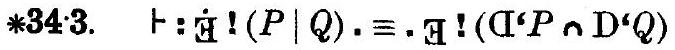
\includegraphics[max width=\textwidth, alt={}, center]{bc1848bf-39e8-4760-b069-9936044df683-133_50_675_213_146}\\
Dem．

$$
\begin{aligned}
& \text { ト.*25.5.つ } \\
& \text { ト:: } \dot{I}!(P \mid Q) . \equiv: .(\mathrm{T} x, y) . x(P \mid Q) y: . \\
& \text { [*34•1] } \quad \equiv: .(\mathbb{H} x, y):(\mathbb{H} z) . x P z . z Q y \text { :. } \\
& \text { [*11'27] } \quad \equiv: .(\text { 月 } x, y, z) . x P z . z Q y: . \\
& \text { [*11•24] } \quad \equiv: .\left(\mathrm{H}^{z, x, y}\right) . x P z . z Q y \text { :. } \\
& \text { [*11•27] } \equiv: .(\mathbb{g} z):(\mathbb{H} x, y) . x P z . z Q y: . \\
& \text { [*11:54] } \equiv: .(\mathrm{Hz}): .\left(\mathrm{H}^{x}\right) . x P z:(\mathrm{H} y) . z Q y: . \\
& {[* 33 \cdot 13 \cdot 131] \equiv: .(\mathbb{H} z): . z \in \mathbb{G} \checkmark P . z \in \mathrm{D}^{6} Q: .} \\
& {[* 2233] \quad \equiv:(\mathrm{H} z): . z \in \mathbb{C}{ }^{\prime} P \cap \mathrm{D}^{\prime} Q: .} \\
& \text { [*24:5] } \quad \equiv: \text { 異! }\left(\mathbb{C}^{\prime} P \cap D^{\prime} Q\right):: \supset \vdash \text {. Prop }
\end{aligned}
$$

＊34：301． $\mathrm{F}: \mathrm{G}^{\prime} P \cap \mathrm{D}^{\prime} Q=\Lambda . \equiv P \mid Q=\dot{\Lambda}$［＊34：3．Transp］\\
＊34：302． $\mathrm{F}: C^{\prime} P \cap C^{\prime} Q=\Lambda$. J．$P|Q=\dot{\Lambda} . Q| P=\dot{\Lambda}$\\
Dem．

$$
\begin{aligned}
& \text { ト. } * 33 \cdot 16 \cdot \supset \vdash: \mathrm{Hp} \cdot \supset \cdot \mathrm{G}^{\top} P \cap \mathrm{D}^{\top} Q=\Lambda \cdot \mathrm{G}^{\top} Q \cap \mathrm{D}^{\top} P=\Lambda . \\
& {[* 34 \cdot 301] \quad \supset \cdot P|Q=\dot{\Lambda} \cdot Q| P=\dot{\Lambda}: \supset \vdash \cdot \text { Prop }} \\
& \text { 卜: 企! }(P \mid Q) \cdot \supset \cdot \text { ர่! } P \cdot \text { 守! } Q
\end{aligned}
$$

Dem．

$$
\begin{aligned}
& \text { [*3324] ɔ.स्⿱冖\zh23⿱⿱一𫝀口廾刂:P. 迁!Q: つト.Prop }
\end{aligned}
$$

＊34．32．$\vdash: P=\dot{\Lambda} . \mathrm{v} . Q=\dot{\Lambda}: \supset . P \mid Q=\dot{\Lambda} \quad$［＊34．31．Transp．＊25．51］\\
＊34．33．$\vdash: x \in \mathrm{D}^{6} R . \equiv x(R \mid \breve{R}) x$\\
Dem．

$$
\begin{aligned}
\vdash \cdot * 33 \cdot 13 . \text { ว। }: x \in \mathrm{D}^{\prime} R & \equiv(\mathrm{H} y) \cdot x R y . \\
{[* 4 \cdot 24] } & \equiv .(\mathrm{H} y) \cdot x R y \cdot x R y . \\
{[* 31 \cdot 11] } & \equiv .(\mathrm{H} y) \cdot x R y \cdot y \breve{R} x . \\
{[* 34 \cdot 1] } & \equiv . x(R \mid \breve{R}) x: \supset \vdash . \text { Prop }
\end{aligned}
$$

＊34．34．$\quad$ ：$R$ CP．SCQ．J．R｜SCP｜Q\\
Dem．


\begin{align*}
& \text { ト.*23.1. ɔ :. Hp. ɔ : } x R y . \supset_{x, y} . x P y: y S z . \supset_{y, z} . y Q z: \\
& \text { [*11•2.*10•141] J: } x R y . \text { J. } x P y: y S z . \text { J. } y Q z \text { : } \\
& \text { [*3.47] J:xRy.ySz.J.xPy.yQz }  \tag{1}\\
& \text { ト.(1).*10.11.21.28. ɔ } \\
& \text { । :. Hp. ɔ : (सy). } x R y . y S z . \text { ɔ . (Hy). } x P y . y Q z \text { : } \\
& {[* 34 \cdot 1] \quad \supset: x(R \mid S) z . \supset . x(P \mid Q) z}  \tag{2}\\
& \text { ト.(2).*11113. ɔ…Prop }
\end{align*}


＊3435．ト：守！R．C‘ RCD＇P．ɔ．宜 $!R \mid P$\\
Dem．


\begin{align*}
& \text { ト. } * 33 \cdot 24 \text {. ɔ }: \mathrm{Hp} \text {. ɔ. } \mathrm{H} \text { ! } \mathrm{U}^{\prime} R  \tag{1}\\
& \text { ト. *22621. ɔ : } \mathrm{Hp} . \text { ɔ. } \mathrm{G}^{\prime} R=\mathrm{G}^{\prime} R \cap \mathrm{D}^{\prime} P  \tag{2}\\
& \text { ト. (1). (2). } \supset \text { : Hp. } \supset \text {. H! } \mathbb{T}^{\prime} R \cap D^{\prime} P \text {. } \\
& \text { [*34:3] ɔ. 写! } R \mid P: \supset \vdash \text {. Prop }
\end{align*}


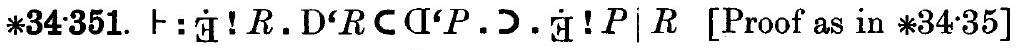
\includegraphics[max width=\textwidth, alt={}, center]{bc1848bf-39e8-4760-b069-9936044df683-134_50_1019_473_224}\\
＊34：36．$\quad$ ㄱ． $\mathrm{D}^{6}(P \mid Q) \subset \mathrm{D}^{6} P . \mathrm{G}^{6}(P \mid Q) \subset \mathrm{G}^{6} Q$\\
Dem．

\[
\begin{array}{ll}
\vdash . * 33 \cdot 13 . \supset \vdash: x \in \mathrm{D}^{6}(P \mid Q) . & \supset:(\mathrm{H} z) . x(P \mid Q) z: \\
{[* 34 \cdot 1]} & \supset:(\mathrm{H} z, y) . x P y . y Q z: \\
{[* 11 \cdot 23]} & \supset:(\mathrm{H} y, z) . x P y . y Q z: \\
{[* 11 \cdot 55 . * 10 \cdot 5]} & \supset:(\mathrm{H} y) . x P y: \\
{[* 33 \cdot 13]} & \supset: x \in \mathrm{D}^{6} P \\
\text { Similarly } \vdash: z \in \mathrm{G}^{6}(P \mid Q) . \supset: z \in \mathrm{G}^{6} P  \tag{2}\\
\text { F.(1).(2).*10.11.J+. Prop }
\end{array}
\]

The following proposition is a lemma for $* 95.31$ ．\\

\includegraphics[max width=\textwidth, alt={}, center]{bc1848bf-39e8-4760-b069-9936044df683-134_54_921_963_233}\\
Dem．


\begin{align*}
& \text { ト. } * 34 \cdot 35 . \supset \vdash: \mathrm{Hp} . \supset . \dot{H}!R \mid Q  \tag{1}\\
& \text { ト. } * 34 \cdot 36 . \supset \vdash: \mathrm{Hp} . \supset . \mathrm{D}^{6}(R \mid Q) \subset \mathrm{C}^{6} P  \tag{2}\\
& \text { ।.(1).(2). } * 34: 351 . \supset \vdash . \text { Prop }
\end{align*}


＊34．37．$\quad$ … $C^{6}(P \mid Q) \subset \mathrm{D}^{6} P^{\prime} \cup \mathrm{U}^{6} Q \quad[* 34 \cdot 36 . * 33 \cdot 161 \cdot * 22 \cdot 72]$\\
＊34：38．$\quad$ ト．$C^{6}(P \mid Q) \subset C^{6} P \cup C^{6} Q \quad[* 3437 . * 33 \cdot 161 . * 22 \cdot 72]$\\
＊344． $\mathrm{F}: b=P^{6} c . c=Q^{6} z$. J．$b=(P \mid Q)^{6} z$\\
Dem．


\begin{align*}
& \text { ト.*30.31. ɔ́:Hp. ɔ.bPc.cQz. } \\
& \text { [*34•1] } \quad \text { J. } b(P \mid Q) z  \tag{1}\\
& \text { ト. } * 3031 . \text { つ } \text { ! }: \text { Hp. } \text { ɔ }: y Q z . \text { J }_{y} . y=c \text { : } \\
& \text { [Fact] } \quad \supset: x P y, y Q z, \mathcal{J}_{x, y}, x P y, y=c \text {. } \\
& \text { [*13.13] } \nu_{x, y \cdot x P c}  \tag{2}\\
& \text { ト. } * 3031 \text {. . } \text { ト }: \text { Hp. } \text { つ }: x P c . \partial_{x} . x=b  \tag{3}\\
& \text { ト.(2).(3). ɔ } \mathrm{F}: \mathrm{Hp} . \supset: x P y . y Q z . \supset_{x, y} . x=b: \\
& \text { [*10.23] } \quad \supset:(\mathrm{H} y) . x P y . y Q z . \supset_{x} . x=b: \\
& \text { [*34•1] } \quad \supset: x(P \mid Q) z . \nu_{x} . x=b  \tag{4}\\
& \text { ト. (1). (4). *30.31. ɔ․ Prop }
\end{align*}


＊34．41．$+: \mathrm{E}!P^{6} Q^{6} z$. J．$P^{6} Q^{6} z=(P \mid Q)^{6} z$\\
Dem．

$$
\begin{array}{ll}
\vdash \cdot * 30 \cdot 52 \cdot \supset \vdash: \mathrm{Hp} \cdot \supset \cdot\left(\mathrm{H}^{b}, c\right) \cdot b=P^{6} c \cdot c=Q^{6} z \cdot \\
{[* 30 \cdot 51 \cdot * 34 \cdot 4]} & \supset \cdot\left(\mathrm{H}^{b}\right) \cdot b=P^{6} Q^{6} z \cdot b=(P \mid Q)^{6} z \cdot \\
{[* 14 \cdot 145]} & \supset \cdot P^{6} Q^{6} z=(P \mid Q)^{6} z: \supset \vdash \cdot \text { Prop }
\end{array}
$$

The above proposition is no longer true if we change the hypothesis into $E!(P \mid Q)^{6} z$ ，since $(P \mid Q)^{6} z$ may exist when $P^{6} Q^{6} z$ does not．Suppose，e．g．， that $Q$ is the relation of child to father，and $P$ the relation of daughter to father．Then $(P \mid Q)^{6} z=$ the granddaughter of $z$ ，but $P^{6} Q^{6} z=$ the daughter of the child of $z$ ．The first exists whenever $z$ has only one granddaughter， while the second requires further that $z$ should have only one child．

For the same reason we do not have

$$
b=(P \mid Q)^{6} z \cdot \supset \cdot\left(\mathrm{G}^{c}\right) \cdot b=P^{6} c \cdot c=Q^{6} z .
$$

This will hold if $P, Q$ are one－many relations（cf．$* 71$ ），but not in general otherwise．\\
＊34．42．$\vdash:(z) \cdot R^{\prime} z=P^{\prime} Q^{\prime} z \cdot$ J $\cdot R=P \mid Q$\\
Dem．


\begin{align*}
& \vdash \cdot * 14 \cdot 21 . \quad \supset \vdash: \text { Hp } . \supset:(z) \cdot \text { E }!R^{6} z:(z) \cdot \text { E }!P^{6} Q^{6} z  \tag{1}\\
& \vdash \cdot(1) \cdot * 34 \cdot 41 \cdot \supset \vdash: \text { Hp } . \supset:(z) \cdot R^{6} z=(P \mid Q)^{6} z: \\
& {[* 30 \cdot 42 .(1)] \quad \supset: R=P \mid Q: \supset \vdash . \text { Prop }}
\end{align*}


＊34：5．$\quad$ ：$x R^{2} y . \equiv .(\mathrm{Hz}) . x R z . z R y \quad$［＊34•1．（＊34：02）］\\
＊34．51． 卜：$x R^{3} y$ ．$\equiv$ ．（ु $z, w$ ）．$x R z . z R w . w R y$\\
Dem．

$$
\begin{aligned}
& \vdash \cdot * 34 \cdot 1 \cdot(* 34 \cdot 03) \cdot \supset \\
& \vdash: \cdot x R^{3} y \cdot \equiv:(\mathrm{H} w) \cdot x R^{2} w \cdot w R y: \\
& {[* 34 \cdot 5] \quad \equiv:(\mathrm{H} w):\left(\mathrm{H}^{z}\right) \cdot x R z \cdot z R w: w R y:} \\
& {[* 11 \cdot 55] \quad \equiv:\left(\mathrm{H}^{w}, z\right) \cdot x R z \cdot z R w \cdot w R y:} \\
& {[* 11 \cdot 2] \quad \equiv:\left(\mathrm{H}^{z}, w\right) \cdot x R z \cdot z R w \cdot w R y: . \supset \text { ।. Prop }}
\end{aligned}
$$

＊34：52． ト $. R^{3}=R \mid R^{2}$［＊34：21］\\
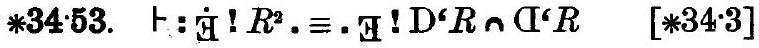
\includegraphics[max width=\textwidth, alt={}, center]{bc1848bf-39e8-4760-b069-9936044df683-135_48_759_1354_155}\\
＊34：531．$+\mathrm{D}^{\wedge} R \cap \mathbb{G}^{\wedge} R=\Lambda . \equiv R^{2}=\dot{\Lambda} \quad$［＊34：53．Transp］\\
＊34：54． －$x R x$ ．ɔ．$x R^{2} x$\\
Dem．

$$
\begin{array}{ll}
\vdash . * 4 \cdot 24 . \text { つ }: x R x . \text { J. } x R x . x R x . \\
{[* 10 \cdot 24]} & \text { J. (H } y) . x R y . y R x . \\
{[* 34 \cdot 5]} & \text { J. } x R^{2} x: \text { ɔ } . \text { Prop }
\end{array}
$$

＊3455．$+: R^{2}$ C $S . \equiv: x R y . y R z . \nu_{x, y, z} . x S z \quad$［＊34．5．＊10．23］\\
＊34：56．ト． $\mathrm{D}^{6} R^{2} \subset \mathrm{D}^{6} R$. I ${ }^{6} R^{2} \subset \mathrm{C}^{6} R . C^{6} R^{2} \subset C^{6} R \quad[* 34.36 .38]$\\
＊346．$\quad$ ㅏ．$(R \dot{n} S)^{2} € R^{2} \dot{n} S^{2}$\\
Dem．

$$
\begin{array}{ll}
\vdash \cdot * 34 \cdot 5 \cdot \supset \vdash: x(R \dot{\Omega})^{2} y \cdot & \equiv:(\mathrm{H} z) \cdot x(R \dot{\text { i } S) z \cdot z(R \dot{\text { i } S)} y:} \\
{[* 23 \cdot 33 \cdot * 10 \cdot 281]} & \equiv:(\mathrm{H} z) \cdot x R z \cdot x S z \cdot z R y \cdot z S y: \\
{[* 4 \cdot 3 \cdot * 10 \cdot 281]} & \equiv:(\mathrm{H} z) \cdot x R z \cdot z R y \cdot x S z \cdot z S y:
\end{array}
$$

\[
\begin{array}{ll}
{[* 10 \cdot 5]} & \supset:\left(\mathrm{H}^{2}\right) \cdot x R z \cdot z R y:(\mathrm{H} z) \cdot x S z \cdot z S y: \\
{[* 34 \cdot 5]} & \supset: x R^{2} y \cdot x S^{2} y: \\
{[* 23 \cdot 33]} & \supset: x\left(R^{2} \dot{\circ} S^{2}\right) y  \tag{1}\\
\text { ト.(1).*11.11.} \supset+. P r o p &
\end{array}
\]

＊34．62．

$$
\text { F } \cdot(R \mho S)^{2}=R^{2} \mho R|S \mho S| R \mho S^{2}
$$

Dem．

$$
\begin{aligned}
\vdash \cdot * 34 \cdot 26 . \text { コト. }(R \cup S)^{2} & =R|(R \cup S) \cup S|(R \cup S) \\
& =R^{2} \cup R|S \cup S| R \cup S^{2} . \text { ɔ } . \text { Prop } \\
{[* 34 \cdot 25] } &
\end{aligned}
$$

The above proposition is a lemma for $* 160 \cdot 51$ ，as is also $* 34 \cdot 73$ ，which employs the above proposition．\\
＊34．63．

$$
\vdash \cdot \operatorname{Cnv}^{6}\left(R^{2}\right)=\left(\operatorname{Cnv} v^{6} R\right)^{2}
$$

Dem．

$$
\begin{aligned}
& \text { ト.*31.131. ɔ } \\
& \text { ト: } . x\left\{\mathrm{Cnv}^{c}\left(R^{2}\right)\right\} y . \equiv: y R^{2} x: \\
& \text { [*34:5] } \equiv:\left(\mathrm{H}^{z}\right) . y R z . z R x: \\
& {[* 31 \cdot 131 \cdot * 10 \cdot 281] \equiv:(\mathrm{H} z) \cdot x R z \cdot z \vec{R} y:} \\
& {[* 31 \cdot 131 . * 34 \cdot 5] \quad \equiv: x\left(\mathrm{Cnv}^{4} R\right)^{2} y: \text { ว!. Prop }}
\end{aligned}
$$

＊347．$\quad$ ト． $\mathrm{Cnv}^{\prime}(S \mid \breve{S})=S \mid \breve{S}$\\
Dem．

$$
\begin{aligned}
\vdash \cdot * 34 \cdot 2 . \supset \vdash . \mathrm{Cnv}^{\prime}(S \mid \breve{S}) & =\left(\mathrm{Cnv}^{\breve{S}} \breve{S}\right) \mid \breve{S} \\
{[* 34 \cdot 202] } & =S \mid \breve{S} . \supset \vdash . \text { Prop }
\end{aligned}
$$

Thus $S \mid \breve{S}$ is always a symmetrical relation，i．e．one which is equal to its converse．\\
＊34•701． ト $^{\prime} \operatorname{Cnv}^{\prime}(\breve{S} \mid S)=\breve{S} \mid S \quad$［＊34•2203］\\
＊34：702． ᄀ $. C^{6}(S \mid \breve{S})=\mathrm{D}^{6} S$\\
Dem．


\begin{align*}
& \text { ト. } * 3437 \text {. } \supset \text { ト } . C^{6}(S \backslash \breve{S}) \subset \mathrm{D}^{6} S \cup \mathrm{G}^{\breve{S}} \\
& \text { [*33*21] CD'S }  \tag{1}\\
& \text { ト.*33-13. ɔ : } x \in \mathrm{D}^{\prime} S . \supset .(\mathrm{H} y) . x S y . \\
& \text { [*31•11] ɔ.(Hy).xSy.yS } x \text {. } \\
& \text { [*34•1] } \quad \supset . x(S \mid \breve{S}) x \text {. } \\
& \text { [*33.17] } \quad \text { ɔ } x \in C^{6}(S \mid \breve{S})  \tag{2}\\
& \text { ト.(1).(2).*10.11.ɔ‥Prop }
\end{align*}


＊34．703． r．$C^{6}(\breve{S} \mid S)=G^{6} S$［Similar proof］\\
＊34．73．$\vdash: C^{6} P \cap C^{6} Q=\Lambda . \supset .(P \circlearrowleft Q)^{2}=P^{2} \circlearrowleft Q^{2}$\\
Dem．

$$
\begin{aligned}
& \vdash \cdot * 34 \cdot 302 \cdot \supset \vdash: \text { Hp } . \supset \cdot P|Q=\dot{\Lambda} \cdot Q| P=\dot{\Lambda} . \\
& {[* 25 \cdot 24]} \\
& {[* 34 \cdot 62]}
\end{aligned} \begin{aligned}
\supset \cdot P^{2} \cup Q^{2} & =P^{2} \cup P|Q \cup Q| P \cup Q^{2} \\
& =(P \cup Q)^{2}: \supset \vdash . \text { Prop }
\end{aligned}
$$

＊34．8．$\quad$ ：$R=\breve{R} . R^{2} \in R$. つ．$R=R^{2}=R \mid \breve{R}$\\
Dem．


\begin{align*}
& \text { ト. } * 34 \text { : 28. } \quad \supset \vdash: R=\breve{R} . \supset . R^{2}=R \mid \breve{R}  \tag{1}\\
& \text { ト. *34:33. *33.14. ɔㅐ: } x R y . \text { ɔ. } x(R \mid \breve{R}) x  \tag{2}\\
& \text { ト.(1).(2). } \quad \supset \vdash: R=\breve{R} . \supset: x R y . \text { ɔ. } x R^{2} x  \tag{3}\\
& \text { ト.(3).*23.1. ɔト:. } R=\breve{R} . R^{2} \boxminus R . \supset: x R y . \supset . x R x \text { : } \\
& \text { [*4•7] ১:xRy.ɔ.xRx.xRy. } \\
& \text { [*10.24.*34.5] } \\
& \text { ɔ. } x R^{2} y  \tag{4}\\
& \text { ト.(4).*11.113. ɔ}=\mathrm{Hp} . \supset . R \in R^{2}  \tag{5}\\
& \text { ト.*3.27. } \quad \supset \vdash: \mathrm{Hp} . \supset . R^{2} \in R  \tag{6}\\
& \text { ト.(5).(6).*23.41. ɔ : Hp. ɔ. } R=R^{2}  \tag{7}\\
& \text { ト.(1).(7). ɔ…Prop }
\end{align*}


The hypothesis of the above proposition is the hypothesis that $R$ is symmetrical（ $R=\breve{R}$ ）and transitive（ $R^{2} \subset R$ ）．These are the formal properties of those relations which can suitably be regarded as expressing equality in some respect．\\
＊34：81．$\vdash: R=\breve{R} \cdot R^{2}$ € $R . \equiv R=\breve{R} \cdot R^{2}=R \quad[* 34 \cdot 8 \cdot * 4 \cdot 71]$\\
The following propositions are lemmas for $* 34 \cdot 85$ ，which is used in $* 72 \cdot 64$ ，\\
＊34．82． $\mathrm{F}: . R=\breve{R} . R^{2} \in R . \supset: x \in \mathrm{D}^{\prime} R . \equiv . x R x$\\
Dem．


\begin{align*}
& \text { ト. } * 34 \cdot 33 . \text { ɔ।: } x \in \mathrm{D}^{6} R . \equiv . x(R \mid \breve{R}) x  \tag{1}\\
& \text { ।. } * 34 \cdot 8 . \text { ɔ }: . \text { Hp. } \text { つ: } x(R \mid \breve{R}) x . \equiv . x R x  \tag{2}\\
& \text { ।. }(1) .(2) . \text { つ } . \text { Prop }
\end{align*}


＊34：83． ト $: R=\breve{R} \cdot R^{2} \subset R \cdot x R y \cdot \supset \cdot \overleftarrow{R}^{6} x=\overleftarrow{R^{6}} y$\\
Dem．


\begin{align*}
& \text { ト.*31-11. ɔㅡ: Hp. ɔ: } y R x: \\
& \text { [*3.2] つ:xRz.ɔ.yRx.xRz. } \\
& \text { [*34.55.Hp] ɔ.yRz }  \tag{1}\\
& \text { ト.*3.2. ɔト:. Hp. ɔ: } y R z . \text { ɔ. } x R y . y R z \text {. } \\
& \text { [*34:55.Hp] ɔ.xRz }  \tag{2}\\
& \text { ト.(1).(2). ɔ : : Hp. ɔ : } x R z . \equiv . y R z \text { : } \\
& {[* 10 \cdot 11 \cdot 21 . * 20 \cdot 15 . * 32 \cdot 111] \supset: \overleftarrow{R}^{6} x=\overleftarrow{R}^{6} y: . \text { ว!. Prop }}
\end{align*}


＊3484．$\leqslant: R=\breve{R} \cdot R^{2} \oplus R \cdot y \in \mathrm{D}^{\prime} R \cdot \overleftarrow{R^{\prime}} x=\overleftarrow{R^{\prime}} y \cdot \supset \cdot x R y$\\
Dem．


\begin{align*}
& \text { ।.*34.82. ɔト:Hp.ɔ.yRy }  \tag{1}\\
& \text { ト . } * 32181 . * 2031 . \text { ɔ }: . \mathrm{Hp} . \text { つ }: x R z . \equiv_{z} . y R z \text { : } \\
& \text { [*10.1] } \quad \text { J: } x R y . \equiv . y R y  \tag{2}\\
& \text { ト. (1). (2). ɔト. Prop }
\end{align*}


＊34841．$\vdash: R=\breve{R} \cdot R^{2} \subset R \cdot x \in \mathrm{D}^{6} R \cdot \overleftarrow{R}^{6} x=\overleftarrow{R}^{6} y \cdot \nu \cdot x R y$\\
Dem．

$$
\begin{array}{ll}
\vdash . * 34 \cdot 84 \frac{y, x}{x, y} . \text { つト: Hp. ɔ. } y R x . & \\
{[* 31 \cdot 11 . \mathrm{Hp}]} & \text { ɔ. } x R y: \text { ɔ } . \text { Prop }
\end{array}
$$

＊3485．$\vdash: R=\breve{R} \cdot R^{2} \subset R \cdot \supset: x R y \cdot \equiv \cdot x \in \mathrm{D}^{\prime} R \cdot \overleftarrow{R}^{\prime} x=\overleftarrow{R}^{\prime} y$ ［＊34．83．841．＊33．14］

\section*{*35. RELATIONS WITH LIMITED DOMAINS AND CONVERSE DOMAINS}
\section*{Summary of *35.}
In this section, we have to consider the relation derived from a given relation $R$ by limiting either its domain or its converse domain to members of some assigned class. A relation $R$ with its domain limited to members of $\alpha$ is written " $\alpha \upharpoonleft R$ "; with its converse domain limited to members of $\beta$, it is written " $R \upharpoonright \beta$ "; with both limitations, it is written " $\alpha \mid R \upharpoonright \beta$." Thus e.g. "brother" and "sister" express the same relation (that of a common parentage), with the domain limited in the first case to males, in the second to females. "The relation of white employers to coloured employees" is a relation limited both as to its domain and as to its converse domain. We put

\section*{*35.01. $\quad \alpha \upharpoonleft R=\hat{x} \hat{y}(x \in \alpha . x R y) \quad$ Df}
with similar definitions for $R \upharpoonright \alpha$ and $\alpha\rceil R \uparrow \beta$.\\
A particularly important case is the case in which the same limitation is imposed on the domain and on the converse domain, i.e. where we have a relation of the form " $\alpha \upharpoonleft R \upharpoonleft \alpha$." In this case, the limitation to members of $\alpha$ may be more briefly stated as being imposed on the field. For this case, it is convenient to adopt " $R$ 个 $\alpha$ " as an alternative notation. This case will be considered in $* 36$.

It is convenient to consider in the present connection the relation between $x$ and $y$ which is constituted by $x$ being a member of $\alpha$ and $y$ being a member of $\beta$. This relation will be denoted by " $\alpha \uparrow \beta$." Thus we put

\section*{*35.04. $\alpha \uparrow \beta=\hat{x} \hat{y}(x \in \alpha \cdot y \in \beta) \quad$ Df}
The chief importance of relations with limited fields arises in the theory of series. Given a series generated by a relation $R$, let $\alpha$ be a class consisting of part of this series. Then $\alpha$ is the field of the relation $\alpha \upharpoonleft R \uparrow \alpha$ or $R[\alpha$, and it is this relation which is the generating relation of the series of members of $\alpha$ in the same order which they have as parts of the original series. Thus parts of a series, considered not merely as classes but as series, are dealt with by means of serial relations with limited fields.

Relations with limited domains are not nearly so much used as relations with limited converse domains. Relations with limited converse domains play a great part in arithmetic, especially in establishing the formal laws. What is wanted in such cases is a one-one relation correlating two classes or two series. That is, we want a relation such that not only does $R^{\prime} y$ exist whenever $y \in G^{\prime} R$, but also $\breve{R}^{\prime} x$ exists whenever $x \in \mathrm{D}^{\prime} R$. The kind of relation which is most frequently found to effect such a correlation is some such relation as D\\
or G or $C$, or some other constant relation for which we always have $\mathrm{E}!R^{6} y$, with its converse domain so limited that, subject to the limitation, only one value of $y$ gives any given value of $R^{\prime} y$. Thus for example let $\lambda$ be a class of relations no two of which have the same domain; then $\mathrm{D} \upharpoonright \lambda$ will give a oneone correlation of these relations with their domains: if $R, S \in \lambda$, we shall have

$$
\mathrm{D}^{\prime} R=\mathrm{D}^{\prime} S . \supset . R=S .
$$

We shall also have $\mathrm{D}^{6} R=(\mathrm{D} \upharpoonright \lambda)^{6} R$ and $\mathrm{D}^{6} S=(\mathrm{D} \upharpoonright \lambda)^{6} S$. Moreover the converse domain of $\mathrm{D} \upharpoonright \lambda$ is $\lambda$, and the domain of $\mathrm{D} \upharpoonright \lambda$ is the class of domains of members of $\lambda$. Thus $\mathrm{D} \upharpoonright \lambda$ gives a one-one correlation of $\lambda$ with the domains of members of $\lambda$. It is chiefly in such ways that relations with limited converse domains are useful.

For purposes of reference, a great many propositions are given in the present number, but the propositions that will be used frequently are comparatively few. Among these are the following:\\
*3521. ト. $\alpha \upharpoonleft R \uparrow \beta=(\alpha \upharpoonleft R) \uparrow \beta=\alpha 1(R \uparrow \beta)$\\
*35.31. F. $(R \upharpoonright \alpha) \upharpoonright \beta=R \upharpoonright(\alpha \cap \beta)$\\
*35.354. $\vdash \cdot(R \upharpoonright \alpha)|S=R| \alpha \mid S$\\
I.e. in a relative product it makes no difference whether we limit.the converse domain of the first factor, or the domain of the second.\\
*35•412. ↓ . $R \upharpoonright\left(\beta \cup \beta^{\prime}\right)=R \upharpoonright \beta v R \upharpoonright \beta^{\prime}$\\
*35452. $\mathrm{F}: \mathbb{G}^{\prime} R \subset \beta . \supset . R \uparrow \beta=R$\\
*35.48. $\quad$ s: $\mathbb{C}(P \subset \alpha$. J. $P|(\alpha \mid R)=P| R$\\
*35.52. $\quad$ … $\operatorname{Cnv}^{\prime}(R \upharpoonright \beta)=\beta \upharpoonleft \breve{R}$\\
*35.61. $\quad$ F. $\mathrm{D}^{\prime}(\alpha \mid R)=\alpha \cap \mathrm{D}^{\prime} R$\\
*35.64. $\quad$ … $\mathrm{G}^{\prime}(R \uparrow \beta)=\beta \cap \mathrm{G}^{\prime} R$\\
*35.65. $\quad$ : $\beta \subset \mathbb{C}^{\prime} R$. ɔ . $\mathbb{G}^{\prime}(R \uparrow \beta)=\beta$\\
The hypothesis $\beta \subset \mathrm{C}^{\prime} R$ is fulfilled in the great majority of cases in which we have occasion to use $R \upharpoonright \beta$.\\
*35.66. ㅏ: $\mathbb{C}{ }^{\top} R \subset \beta . \equiv . R \uparrow \beta=R$\\
*35.7. $\quad \vdash: \phi\left\{(R \uparrow \beta)^{6} y\right\} . \equiv . y \in \beta . \phi\left(R^{6} y\right)$\\
This proposition is used very frequently, owing to the fact that limitation of the converse domain is chiefly applied to such relations as give rise to descriptive functions (e.g. D, $\mathbb{T}, C$ ).\\
*35.71. ト $: . y \in \beta . \partial_{y} . R^{6} y=S^{6} y: \partial . R \uparrow \beta=S \uparrow \beta$\\
This proposition is useful for a reason similar to that which makes *35.7 useful.\\
*35.82. $\quad$ ‥ $\alpha \uparrow \beta=\alpha \uparrow \dot{V} \uparrow \beta$\\
Owing to this proposition, the properties of $\alpha \uparrow \beta$ can be deduced from the already proved properties of $\alpha \upharpoonleft R \upharpoonright \beta$, by putting $R=\dot{\mathrm{V}}$.

The relation＂$\alpha \uparrow \beta$＂is what may be called an＂analysable＂relation，i．e．it holds between $x$ and $y$ when $x \in \alpha$ and $y \in \beta$ ，i．e．when $x$ has a property inde－ pendent of $y$ ，and $y$ has a property independent of $x$ ．\\
＊3585． ト：$A!\beta$ ．$\supset$ ． $\mathrm{D}^{\prime}(\alpha \uparrow \beta)=\alpha$\\
＊3586． F：$H$ ！$\alpha$. つ．$G^{\prime}(\alpha \uparrow \beta)=\beta$\\
If either $\alpha$ or $\beta$ is null，so is $\alpha \uparrow \beta(* 35 \cdot 88)$ ．

\begin{center}
\begin{tabular}{lll}
＊35．01． & $\alpha \uparrow R=\hat{x} \hat{y}(x \in \alpha \cdot x R y)$ & Df \\
＊35．02． & $R \uparrow \beta=\hat{x} \hat{y}(x R y \cdot y \in \beta)$ & Df \\
＊35．03． & $\alpha \uparrow R \uparrow \beta=\hat{x} \hat{y}(x \in \alpha \cdot x R y \cdot y \in \beta)$ & Df \\
＊35．04． & $\alpha \uparrow \beta=\hat{x} \hat{y}(x \in \alpha \cdot y \in \beta)$ & Df \\
＊35．05． & $R^{\prime} x \uparrow \beta=\left(R^{\prime} x\right) \uparrow \beta$ & Df \\
\end{tabular}
\end{center}

The last definition serves merely for the avoidance of brackets．\\
＊35－1．$\quad \vdash: x(\alpha \upharpoonleft R) y . \equiv . x \in \alpha . x R y \quad[* 213 .(* 35.01)]$\\
$* 35 \cdot 101 . \vdash: x(R \uparrow \beta) y . \equiv \ldots R y . y \in \beta$\\
＊35－102． $\mathrm{F}: x(\alpha \upharpoonleft R \uparrow \beta) y . \equiv x \in \alpha . x R y . y \in \beta$\\
＊35•103． $\mathrm{F}: x(\alpha \uparrow \beta) y . \equiv . x \in \alpha . y \in \beta$\\
＊35－11．ト．$\alpha \upharpoonleft R \uparrow \beta=(\alpha \upharpoonleft R) \dot{\wedge}(R \uparrow \beta)$\\
Dem．\\
ト ．$* 35 \cdot 102$. つ $: x(\alpha \uparrow R \uparrow \beta) y . \equiv . x \in \alpha . x R y . y \in \beta$ ．\\
［＊4－24］$\quad \equiv x \in \alpha . x R y . x R y . y \in \beta$ ．\\
［＊35•1•101］\\
$\equiv . x(\alpha \upharpoonleft R) y . x(R \uparrow \beta) y$ ．\\
［＊23．33］\\
$\equiv . x\{(\alpha \upharpoonleft R) \dot{\wedge}(R \uparrow \beta)\} y:$ ɔト．Prop\\
＊35－12．$\quad$ ㄱ．$(\alpha \upharpoonleft R) \dot{n}(S \uparrow \beta)=\alpha 1(R \dot{\cap} S) \uparrow \beta$\\
Dem．\\
ト.$* 2333$. つ $: x\{(\alpha \upharpoonleft \dot{R}) \dot{n}(S\lceil\beta)\} y . \equiv . x(\alpha \upharpoonleft R) y . x(S\lceil\beta) y$.\\
［＊35•1•101］\\
$\equiv . x \in \alpha . x R y . x S y . y \in \beta$.\\
［＊23：33］\\
$\equiv . x \in \alpha . x\left(R \cap \dot{\text { S }}_{\text {® }}\right) y . y \in \beta$ ．\\
［＊35•102］\\
$\equiv . x\{\alpha\}(R \cap S) \uparrow \beta\} y: \supset \vdash$ ．Prop\\
＊35．13．$\quad$ ㅏ．$(\alpha \upharpoonleft R) \dot{\cap}(\beta \upharpoonleft S)=(\alpha \cap \beta) 1(R \dot{\cap} S)$\\
Dem：

$$
\begin{array}{ll}
\vdash \cdot * 23 \cdot 33 . \supset \vdash: x\{(\alpha \upharpoonleft R) \dot{\cap}(\beta \upharpoonleft S)\} y & \equiv \ldots(\alpha \upharpoonleft R) y . x(\beta \upharpoonleft S) y . \\
{[* 35 \cdot 1]} & \equiv x \in \alpha . x R y . x \in \beta . x S y . \\
& \equiv x \epsilon(\alpha \cap \beta) . x(R \dot{n} S) y . \\
{[* 22 \cdot 33 . * 23 \cdot 33]} & \equiv x\{(\alpha \cap \beta) 1(R \dot{n} S)\} y: \supset \vdash . \text { Prop } \\
{[* 35 \cdot 1]} & \equiv . x\{
\end{array}
$$

＊35•14．$\quad \vdash .(R \upharpoonright a) \dot{\cap}(S \upharpoonright \beta)=(R \dot{\cap} S) \upharpoonright(\alpha \cap \beta) \quad$［Similar proof to＊35•13］\\
＊35：15．$\quad$ ‥ $\left.(\alpha \upharpoonleft R \uparrow \beta) \dot{n}\left(\alpha^{\prime} \upharpoonleft S \uparrow \beta^{\prime}\right)=\left(\alpha \cap \alpha^{\prime}\right)\right\}(R \dot{\cap} S) \uparrow\left(\beta \cap \beta^{\prime}\right)$\\
Dem．\\
ト．＊3511．ɔ

$$
\begin{array}{ll}
\text { l. }(\alpha \upharpoonleft R \uparrow \beta) \dot{n}\left(\alpha^{\prime} 1 S \uparrow \beta^{\prime}\right) & =(\alpha \upharpoonleft R) \dot{n}(R \uparrow \beta) \dot{n}\left(\alpha^{\prime} 1 S\right) \dot{n}\left(S \uparrow \beta^{\prime}\right) \\
{[* 35 \cdot 13 \cdot 14]} & =\left\{\left(\alpha \cap \alpha^{\prime}\right) 1(R \dot{n} S)\right\} \dot{n}\left\{(R \dot{n} S) \uparrow\left(\beta \cap \beta^{\prime}\right)\right\} \\
{[* 35 \cdot 11]} & =\left\{\left(\alpha \cap \alpha^{\prime}\right) 1(R \dot{n} S) \uparrow\left(\beta \cap \beta^{\prime}\right)\right\} . \supset \vdash . \text { Prop }
\end{array}
$$

＊3516．… $(\alpha \upharpoonleft R) \dot{\cap} S=\alpha \upharpoonleft(R \dot{\cap} S)=R \dot{\cap} \alpha \upharpoonleft S \quad$［Similar proof to＊35．13］\\
＊35．17．$\quad \vdash .(R \uparrow \beta) \dot{n} S=(R \dot{n} S) \uparrow \beta=R \dot{n} S \uparrow \beta \quad$［Similar proof to＊35．13］\\
＊3518．$\quad$ ㅏ．$(\alpha \upharpoonleft R \uparrow \beta) \dot{n} S=\alpha \upharpoonleft(R \dot{n} S) \uparrow \beta=R \dot{n} \alpha \upharpoonleft S \uparrow \beta$\\
［Similar proof to $* 35 \cdot 15$ ］\\
＊35．21． F $. \alpha \upharpoonleft R \uparrow \beta=(\alpha \upharpoonleft R) \uparrow \beta=\alpha 1(R \uparrow \beta)$\\
Dem．

\[
\begin{array}{ll}
\vdash . * 35 \cdot 102 . \supset \vdash: x(\alpha \uparrow R \uparrow \beta) y & \equiv . x \in \alpha . x R y . y \in \beta . \\
{[* 35 \cdot 1]} & \equiv . x(\alpha \uparrow R) y . y \in \beta . \\
{[* 35 \cdot 101]} & \equiv . x\{(\alpha \uparrow R) \uparrow \beta\} y \\
\vdash . * 35 \cdot 102 . \supset \vdash: x(\alpha \uparrow R \uparrow \beta) y & \equiv . x \in \alpha . x R y . y \in \beta . \\
{[* 35 \cdot 101]} & \equiv . x \in \alpha . x(R \uparrow \beta) y . \\
{[* 35 \cdot 1]} & \equiv . x\{\alpha \uparrow(R \uparrow \beta)\} y \tag{2}
\end{array}
\]

ト.(1).(2).ɔ . Prop\\
＊35．22． ト．$(\alpha \upharpoonleft R) \mid S=\alpha \upharpoonleft(R \mid S)$\\
Dem．

$$
\begin{aligned}
& \text { ト. *34:1. ɔㅐ: } x\{(\alpha \mid R) \mid S\} y . \equiv:(H z) . x(\alpha \upharpoonleft R) z . z S y: \\
& \text { [*35•1] } \equiv:\left(\mathrm{H}^{z}\right) . x \in \alpha . x R z . z S y \text { : } \\
& \text { [*1035] } \equiv: x \in \alpha:(\mathbb{H} z) . x R z . z S y \text {. } \\
& \text { [*34.1] } \equiv: x \in \alpha . x(R \mid S) y \text { : } \\
& \text { [*35.1] } \equiv: \infty\{\alpha \mid(R \mid S)\} y: . \supset \vdash \text {.Prop }
\end{aligned}
$$

＊35．23．$\quad$ F．$S \mid(R \uparrow \beta)=(S \mid R) \uparrow \beta \quad$［Similar proof to $* 3522$ ］\\
＊35．24 $\quad \alpha|R| S=(\alpha \mid R) \mid S$ Df\\
＊35．25．$\quad S \mid R \uparrow \beta=(S \mid R) \uparrow \beta \quad$ Df\\
＊35．26．$f .(\alpha \upharpoonleft R) \mid(S \upharpoonleft \beta)=\alpha 1(R \mid S) \uparrow \beta=\{\alpha 1(R \mid S)\} \uparrow \beta=\alpha 1\{(R \mid S) \uparrow \beta\}$

$$
\begin{aligned}
& =\{(\alpha \uparrow R) \mid S\}\lceil\beta=\alpha \uparrow\{R \mid(S \uparrow \beta)\} \\
& =(\alpha \uparrow R \mid S) \uparrow \beta=\alpha \uparrow(R \mid S \uparrow \beta)
\end{aligned}
$$

Dem．

\[
\begin{array}{ll}
\vdash \cdot * 341.2 \vdash: x\{(\alpha \uparrow R) \mid(S \uparrow \beta)\} y & \equiv:\left(H^{z}\right) \cdot x(\alpha \uparrow R) z \cdot z(S \uparrow \beta) y: \\
{[* 35 \cdot 1 \cdot 101]} & \equiv:\left(H^{z}\right) \cdot x \in \alpha \cdot x R z \cdot z S y \cdot y \in \beta: \\
{[* 10 \cdot 35]} & \equiv: x \in \alpha \cdot y \epsilon \beta:\left(H^{z}\right) \cdot x R z \cdot z S y: \\
{[* 34 \cdot 1]} & \equiv: x \in \alpha \cdot x(R \mid S) y \cdot y \in \beta: \\
{[* 35 \cdot 102]} & \equiv: x\{\alpha \mid(R \mid S) \uparrow \beta\} y  \tag{1}\\
\vdash \cdot(1) \cdot * 35 \cdot 21 \cdot 22 \cdot 23 \cdot(* 35 \cdot 24 \cdot 25) \cdot \text { J } \cdot \text { Prop }
\end{array}
\]

＊35．27．$\quad \alpha \upharpoonleft R \mid S \uparrow \beta=(\alpha \uparrow R \mid S) \uparrow \beta \quad$ Df\\
＊35．31．$\quad \vdash .(R \upharpoonright \alpha) \uparrow \beta=R \upharpoonright(\alpha \cap \beta)$\\
Dem．

$$
\begin{array}{ll}
\vdash . * 35 \cdot 101 . \supset \vdash: x\{(R \upharpoonright \alpha)\lceil\beta\} y & \equiv . x(R \upharpoonright \alpha) y . y \epsilon \beta . \\
{[* 35 \cdot 101]} & \equiv . x R y . y \in \alpha . y \in \beta . \\
{[* 22 \cdot 33]} & \equiv . x R y . y \in \alpha \cap \beta . \\
{[* 35 \cdot 101]} & \equiv . x\{R \upharpoonright(\alpha \cap \beta)\} y: \supset \vdash . \text { Prop }
\end{array}
$$

＊3532．F．$\alpha 1(\beta 1 R)=(\alpha \cap \beta) 1 R$［Proof similar to that of＊35＊31］\\
＊35．33．$\quad \vdash .(\alpha \upharpoonleft R \uparrow \beta) \uparrow y=\{\alpha \uparrow R \uparrow(\beta \cap \gamma)\} \quad$［Proof similar to that of＊35．31］\\
＊35．34．F．$\alpha \upharpoonleft(\beta \upharpoonleft R \upharpoonright \gamma)=\{(\alpha \cap \beta) \upharpoonleft R \upharpoonright \gamma\} \quad$［Proof similar to that of＊35．31］\\
＊3535．$\leqslant \alpha \upharpoonleft R=\left(\alpha \cap D^{\wedge} R\right) \upharpoonleft R$\\
Dem．

$$
\begin{array}{ll}
\vdash \cdot * 35 \cdot 1 . \supset \vdash: x(\alpha \mid R) y & \equiv . x \in \alpha . x R y . \\
{[* 33 \cdot 14]} & \equiv . x \in \alpha . x \in D^{6} R . x R y . \\
{[* 22 \cdot 33 . * 35 \cdot 1]} & \equiv . x\left\{\left(\alpha \cap D^{6} R\right) \upharpoonleft R\right\} y: \supset \vdash . \text { Prop }
\end{array}
$$

＊35351．F．$R \upharpoonright \beta=R \uparrow\left(\beta \cap \mathrm{G}^{4} R\right) \quad$［Proof as in＊35．35］\\
＊35352． 卜．$\alpha \upharpoonleft R \upharpoonright \beta=\left(\alpha \cap \mathrm{D}^{4} R\right) \uparrow R \upharpoonright\left(\beta \cap \mathrm{C}^{4} R\right) \quad$［Proof as in＊3535］\\
＊35354． 卜．$(R \upharpoonright \alpha)|S=R| \alpha \mid S$\\
Dem．

$$
\begin{aligned}
& \text { ト.*34•1.*35:101. } 3 \\
& \vdash: x\{(R \upharpoonright \alpha) \mid S\} z . \equiv .(\mathrm{H} y) . x R y . y \in \alpha . y S z . \\
& \text { [*35.1] } \quad \equiv .(\mathrm{H} y) . x R y . y(\alpha \mid S) z \text {. } \\
& \text { [*34-1] } \equiv x\{R \mid(\alpha \mid S)\} z: \text { ว!. Prop }
\end{aligned}
$$

\$\$

$$
＊3542．$+. \alpha 1(R \mho S)=(\alpha \upharpoonleft R) \cup(\alpha \upharpoonleft S)$[＊351．＊2334]
＊35－421．ト．$(R \cup S) \uparrow \beta=(R \upharpoonright \beta) \cup(S \uparrow \beta)$[＊35－101．＊2334]
＊35－422．F．$\alpha \upharpoonleft(R \mho S) \uparrow \beta=(\alpha \upharpoonleft R \uparrow \beta) \circlearrowleft(\alpha \upharpoonleft S \uparrow \beta)[* 35 \cdot 102 \cdot * 23 \cdot 34]$
＊35．43． ㅏ：$\alpha \subset \beta$ ．ɔ ．$\alpha \upharpoonleft R \in \beta \upharpoonleft R$
Dem．
$$

\[
\begin{aligned}
\vdash \cdot * 35 \cdot 1 . \supset \vdash: \alpha \subset \beta . \supset: x(\alpha \mid R) y, & \equiv . x \in \alpha . x R y . \\
{[* 22 \cdot 1] } & \text { J } . x \in \beta . x R y . \\
& \text { J } . x(\beta \upharpoonleft R) y: . \text { J . Prop }
\end{aligned}
\]

$$
＊35．431．$\leqslant: \beta \subset_{\gamma} . \supset . R \uparrow \beta \subset R \Gamma_{\gamma}$[Proof similar to that of＊35．43]
＊35．432．$+: \alpha C_{\gamma} . \beta \subset \delta$. ɔ.$\alpha \upharpoonleft R \upharpoonright \beta G_{\gamma} \upharpoonleft R \upharpoonright \delta$
[Proof similar to that of＊35＊43]
＊35．44．＋．$\alpha 1 R \in R$
Dem．
$$

\[
\begin{aligned}
\vdash . * 35 \cdot 1 . \text { つ }: x(\alpha \upharpoonleft R) y . & \text { ɔ } . x \in \alpha . x R y . \\
& \text { ɔ } . x R y: \partial \text { ।. Prop }
\end{aligned}
\]

$$
＊35－441． ᄀ.$R \upharpoonright \beta \subset R \quad$[Proof similar to that of＊35－44]
＊35．442． r $. \alpha ~ \mid ~ R \uparrow \beta \subset R$[Proof similar to that of $* 35 \cdot 44$ ]
＊35．451． $\mathrm{F}: \mathrm{D}{ }^{\prime} R$ Ca．ɔ．$\alpha \in R=R$
Dem．
$$

\begin{align*}
& {[* 4 \cdot 36] \quad J: x \in \mathrm{D}^{\prime} R . x R y . \equiv . x \epsilon \mathrm{D}^{\prime} R . x R y . x \epsilon \alpha}  \tag{1}\\
& \text { ト. } * 33 \cdot 14 . * 4 \cdot 71 \text {, } \quad \text { J }: x R y . \equiv \ldots \in \mathrm{D}^{\prime} R . x R y  \tag{2}\\
& \text { ト.(1).(2). ɔ : : Hp. ɔ : } x R y . \equiv . x R y . x \in \alpha \text {. } \\
& \text { [*35.1] } \quad \equiv x(\alpha \mid R) y \text { :. ɔ } \text {. Prop }
\end{align*}

$$
＊35．452． $\mathrm{F}: \mathbb{G}^{\prime} R \subset \beta$. ɔ $R \uparrow \beta=R \quad$[Similar proof]
＊35．453． 1 ： $\mathrm{D}{ }^{\wedge} R \subset \alpha$. J．$\alpha \uparrow R \uparrow \beta=R \uparrow \beta$[Similar proof]
＊35－454． $\mathrm{F}: \mathrm{G}^{\prime} R \subset \beta$. J $. \alpha \dagger R \uparrow \beta=\alpha \uparrow R$[Similar proof]
＊35．46．$\quad$ ：$R$ CS．$D$ ．$\alpha \uparrow R$ C $\alpha \uparrow S$
Dem．
$$

\[
\begin{aligned}
& \vdash . * 23 \cdot 1 . \text { J': Hp. } \text { J: } x R y . \text { J. } x S y: \\
& \text { [Fact] } \quad \text { J: } x \in \alpha . x R y . \supset . x \in \alpha . x S y: \\
& {[* 35 \cdot 1] \quad \supset: x(\alpha \mid R) y . \supset . x(\alpha \mid S) y: . \supset \vdash . \text { Prop }}
\end{aligned}
\]

$$
＊35461． $\mathrm{F}: R \in S$. J．$R \uparrow \beta \subset S \uparrow \beta \quad$[Similar proof]
＊35462．$\vdash: R \subseteq S . \supset . \alpha \uparrow R \uparrow \beta \subset \alpha \uparrow S \uparrow \beta$[Similar proof]
＊35471． $\mathrm{F}: \mathbb{C} ‘ \mathrm{P} \cap \alpha=\Lambda . \supset . P \mid(\alpha \upharpoonleft R)=\dot{\Lambda}$
Dem．
$$

\begin{align*}
& \text { ト.*34•1.つト: } x\{P \mid(\alpha \mid R)\} z . \text { ɔ.(H } y) . x P y . y(\alpha \mid R) z . \\
& \text { [*35.1] ɔ.(Ηy).xPy.yeα.yRz. } \\
& \text { [*33.14.*10.5] ɔ.(Я } y \text { ). } y \in \mathbb{C} P . y \in \alpha \text {. } \\
& \text { [*22:33.*24:5] J. 且! C‘Pnα }  \tag{1}\\
& \text { ト.(1).Transp.*24.51.つ } \\
& \text { k: } \mathbb{C}^{\prime} P \cap \alpha=\Lambda . \supset . \sim x\{P \mid(\alpha \mid R)\} z: \\
& [* 11 \cdot 11 \cdot 3]) \supset f: \mathbb{G}^{\prime} P \cap \alpha=\Lambda . \supset .(x, z) . \sim x\{P \mid(\alpha \upharpoonleft R)\} z \text {. } \\
& \text { [*25.15] } \quad \supset . P \mid(\alpha \mid R)=\dot{\Lambda}: \supset \vdash \text {. Prop }
\end{align*}

$$
＊35．48． $\mathrm{F}: \mathbb{C}<P \subset \alpha$. J．$P|(\alpha \mid R)=P| R$
Dem．
$$

\begin{align*}
& \text { ト. } * 221 \text {. } \supset \vdash: \mathrm{Hp} . \supset: y \in \mathbb{G}^{\wedge} P . \partial_{y} . y \in \alpha: \\
& \text { [*4.71] } \quad J: y \in \mathbb{G}^{c} P . y \in \alpha . \equiv_{y . y \in \mathbb{C}}(P: \\
& \text { [*10311] } \quad \text { : } x P y, y \in \mathbb{G}^{\prime} P, y \in \alpha, \equiv_{y} . x P y, y \in \mathbb{G}^{\prime} P \text { (1) } \tag{2}
\end{align*}

$$
$$

\[
\begin{aligned}
& \text { ト.(1).(2). ɔ :. Hp. ɔ : } x P y . y \in \alpha . \equiv_{y} . x P y \text { : } \\
& \text { [*10.311] } \quad \text { J: } x P y . y \in \alpha . y R z . \equiv_{y} . x P y . y R z \text { : } \\
& \text { [*35.1] J:xPy.y }(\alpha \mid R) z . \equiv_{y} . x P y . y R z \text { : } \\
& \text { [*10.281] } \quad J:(\text { 月 } y) . x P y . y(\alpha \upharpoonleft R) z . \equiv \text { (आ } y \text { ). } x P y . y R z \text { : } \\
& \text { [*34•1] J:x(P|a|R)z. 三. } x(P \mid R) z: . \text { ɔㅏ.Prop }
\end{aligned}
\]

$$
＊35．481． $\mathrm{F}: \mathrm{D}^{\prime} R \subset \beta . \supset .(P \uparrow \beta)|R=P| R$[Similar proof]
＊3551．F． $\mathrm{Cnv}^{6}(\alpha \upharpoonleft R)=\breve{R} \upharpoonright \alpha$
Dem．
$$

\[
\begin{array}{ll}
\vdash . * 31 \cdot 131 . \supset \vdash: x\left\{\text { Cnv }^{6}(\alpha \upharpoonleft R)\right\} y & \equiv . y(\alpha \upharpoonleft R) x . \\
{[* 35 \cdot 1]} & \equiv y \in \alpha \cdot y R x . \\
{[* 31 \cdot 11]} & \equiv . x \breve{R} y . y \in \alpha . \\
{[* 35 \cdot 101]} & \equiv . x(\breve{R} \dagger \alpha) y: \supset \vdash . \text { Prop }
\end{array}
\]

$$
＊35．52．F． $\mathrm{Cnv}^{\prime}(R \uparrow \beta)=\beta 1 \breve{R} \quad$[Proof similar to that of＊35．51]
＊35．53．F． $\mathrm{Cnv}^{\prime}(\alpha \upharpoonleft R \upharpoonright \beta)=\beta \upharpoonleft \breve{R}\lceil\alpha$[Proof similar to that of＊35．51]
＊35．61．$+\mathrm{D}^{4}(\alpha \upharpoonleft R)=\alpha \cap \mathrm{D}^{4} R$
Dem．
$$

\[
\begin{aligned}
\vdash \cdot * 33 \cdot 13 . \supset \vdash: x \in \mathrm{D}^{6}(\alpha \mid R) & \equiv:(\text { H } y) \cdot x(\alpha \mid R) y: \\
{[* 35 \cdot 1] } & \equiv:(\text { H } y) \cdot x \in \alpha \cdot x R y: \\
{[* 10 \cdot 35] } & \equiv: x \in \alpha:(\text { H } y) \cdot x R y: \\
{[* 33 \cdot 13] } & \equiv: x \in \alpha \cdot x \in \mathrm{D}^{6} R: \\
{[* 22 \cdot 33] } & \equiv: x \in\left(\alpha \cap \mathrm{D}^{6} R\right): . \supset \vdash . \text { Prop }
\end{aligned}
\]

$$
＊35．62． $\mathrm{F}: \alpha \mathrm{CD}$ R．J． $\mathrm{D}^{\prime}(\alpha \mid R)=\alpha \quad[* 3561 . * 22.621]$
＊35．63． $\mathrm{F}: \mathrm{D}^{6} R \mathrm{C} \alpha . \equiv \alpha \upharpoonleft R=R$
Dem．
$$

\begin{align*}
& \vdash \cdot * 35 \cdot 61 . \supset \vdash: \alpha \uparrow R=R . \supset . \alpha \cap \mathrm{D}^{\top} R=\mathrm{D}^{\top} R . \\
& {[* 22 \cdot 621] \quad \supset . \mathrm{D}^{\top} R \subset \alpha}  \tag{1}\\
& \vdash .(1) \cdot * 35 \cdot 451 . \supset \vdash . \text { Prop }
\end{align*}

$$
＊35．64．F． $\mathrm{G}^{\prime}(R \uparrow \beta)=\beta \cap \mathrm{G}^{\prime} R$[Proof as in＊35．61]
＊35．641．$\vdash: \alpha \cap \mathrm{D}^{\prime} R=\Lambda . \supset . \alpha \upharpoonleft R=\Lambda \quad[* 3561 . * 33 \cdot 241]$
＊35．642． $\mathrm{F}: \alpha \cap \mathrm{C}^{\prime} R=\Lambda . \supset . R \uparrow \alpha=\Lambda \quad[* 3564 . * 33 \cdot 241]$
＊35．643． $\mathrm{F}: \alpha \cap \mathrm{D}^{\prime} R=\Lambda . \supset . \alpha \dagger(R \cup S)=\alpha \upharpoonleft S[* 35.641 \cdot 42]$
＊35．644． $\mathrm{F}: \alpha \cap \mathbb{C}^{\prime} R=\Lambda . \supset .(R \mho S)\lceil\alpha=S\lceil\alpha \quad[* 35.642 \cdot 421]$
＊35．65． $\mathrm{F}: \beta \subset \mathrm{G}^{\prime} R . \supset . \mathrm{G}^{\prime}(R \uparrow \beta)=\beta \quad[* 3564 . * 22.621]$
＊35．66．$\vdash: \mathbb{C}^{\prime} R \subset \beta . \equiv R \uparrow \beta=R$[Proof as in＊35．63]
＊35．671．$\vdash . \mathrm{D}^{c}(R \mid S)=\mathrm{D}^{c}\left(R \uparrow \mathrm{D}^{c} S\right)$
Dem．
$$

\[
\begin{array}{ll}
\vdash . * 33 \cdot 13 . \supset \vdash: x \in \mathrm{D}^{6}(R \mid S) & \equiv:(\mathrm{H} y) \cdot x(R \mid S) y: \\
\begin{array}{ll}
{[* 34 \cdot 1]} & \equiv:(\mathrm{H} y, z) \cdot x R z \cdot z S y: \\
{[* 11 \cdot 23]} & \equiv:\left(\mathrm{H}^{z}, y\right) \cdot x R z \cdot z S y: \\
{[* 10 \cdot 35]} & \equiv:\left(\mathrm{H}^{z}\right): x R z:(\mathrm{H} y) \cdot z S y: \\
{[* 33 \cdot 13]} & \equiv:\left(\mathrm{H}^{z}\right) \cdot x R z \cdot z \in \mathrm{D}^{6} S: \\
{[* 35 \cdot 101]} & \equiv:\left(\mathrm{H}^{z}\right) \cdot x\left(R \uparrow \mathrm{D}^{6} S\right) z: \\
{[* 33 \cdot 13]} & \equiv: x \in \mathrm{D}^{6}\left(R \uparrow \mathrm{D}^{6} S\right): \text { J F.Prop }
\end{array}
\end{array}
\]

$$
＊35．672． $\mathrm{F} . \mathrm{G}^{\prime}(R \mid S)=\mathrm{G}^{\prime}\left(\mathbb{G}^{\prime} R 1 S\right)$[Similar proof]
＊35．68． $\mathrm{F}: \alpha \cap \beta=\Lambda$. J $.(\alpha 1 R \uparrow \beta)^{2}=\dot{\Lambda}$
Dem．
$$

\[
\begin{aligned}
& \vdash \cdot * 35 \cdot 61 \cdot 64 \cdot 21 . \partial \vdash . \mathrm{D}^{\prime}(\alpha \uparrow R \uparrow \beta) \subset \alpha . \mathrm{G}^{\prime}(\alpha \uparrow R \uparrow \beta) \subset \beta . \\
& {[* 22 \cdot 49 \cdot * 24 \cdot 13] \supset \vdash: \alpha \cap \beta=\Lambda . \supset . \mathrm{D}^{\prime}(\alpha \uparrow R \uparrow \beta) \cap \mathrm{G}^{\prime}(\alpha \uparrow R \uparrow \beta)=\Lambda .} \\
& {[* 34 \cdot 531]} \\
& \supset .(\alpha \uparrow R \uparrow \beta)^{2}=\dot{\Lambda}: \supset \vdash . \text { Prop }
\end{aligned}
\]

$$
＊35．7．$\quad$ ：$\phi\left\{(R \uparrow \beta)^{6} y\right\} . \equiv . y \epsilon \beta . \phi\left(R^{6} y\right)$
This proposition is very often used in the later parts of the work．
Dem．
$$

\begin{align*}
& \text { ト. } * 1421 \text {. } \supset \vdash: \phi\left\{(R \uparrow \beta)^{6} y\right\} \text {. . } \mathrm{E}!(R \uparrow \beta)^{6} y \text {. } \\
& \text { [*33.43] ɔ. } y \in \mathbb{G}^{c}(R \uparrow \beta) \text {. } \\
& \text { [*35.64] ɔ. } y \in \beta  \tag{1}\\
& \text { ト . (1). } * 4 \cdot 71 \text {. } \text { J }: \phi\left\{(R \upharpoonright \beta)^{6} y\right\} \cdot \equiv \cdot y \in \beta \cdot \phi\left\{(R \upharpoonright \beta)^{6} y\right\}  \tag{2}\\
& \text { ト. } * 4 \cdot 73 . * 35 \cdot 101 . \text { つ } \text { ↑ : } y \in \beta \text {. } \text { ɔ }: x(R \uparrow \beta) y . \equiv_{x} . x R y \text { : } \\
& \text { [*14.272] } \quad \supset: \phi\left\{(R \uparrow \beta)^{6} y\right\} . \equiv \phi\left(R^{6} y\right)  \tag{3}\\
& \text { ト.(3). } * 532 . \text { J }: y \in \beta . \phi\left\{(R \uparrow \beta)^{6} y\right\} . \equiv . y \epsilon \beta . \phi\left(R^{6} y\right)  \tag{4}\\
& \text { ト.(2).(4). ɔ́. Prop }
\end{align*}

$$
＊35．71．$+:, y \in \beta . \partial_{y} . R^{6} y=S^{6} y: \partial . R \upharpoonright \beta=S \upharpoonright \beta$
Dem．
$$

\[
\begin{array}{ll}
\vdash . * 4 \cdot 7 . \supset \vdash: . \mathrm{Hp} . & \supset: y \in \beta . \partial_{y} . y \in \beta . R^{6} y=S^{6} y: \\
{[* 35 \cdot 7]} & \supset: y \in \beta . \partial_{y} .(R \uparrow \beta)^{6} y=(S \uparrow \beta)^{6} y: \\
{[* 35 \cdot 64]} & \supset: y \in \mathbb{G}^{6}(R \uparrow \beta) \cup \mathbb{G}^{6}(S \uparrow \beta) . \partial_{y} .(R \uparrow \beta)^{6} y=(S \uparrow \beta)^{6} y: \\
{[* 33 \cdot 45]} & \supset: R \uparrow \beta=S \uparrow \beta: . \supset+. \text { Prop }
\end{array}
\]

$$
＊35．75． F $. \Lambda \upharpoonleft R=R \upharpoonright \Lambda=\Lambda \upharpoonleft R \upharpoonright \beta=\alpha \upharpoonleft R \upharpoonright \Lambda=\dot{\Lambda}$
Dem．
$$

\[
\begin{array}{ll}
\vdash . * 35.61 . & \text { ɔr. } \mathrm{D}^{\prime}(\Lambda \upharpoonleft R)=\Lambda . \\
{[* 33.241]} & \text { ɔr. } \dot{\Lambda}\{R=\dot{\Lambda} \tag{1}
\end{array}
\]

$$
$$

\[
\begin{array}{ll}
\vdash \cdot * 35 \cdot 64 . & \supset \vdash . q^{c}(R \uparrow \Lambda)=\Lambda . \\
{[* 33 \cdot 241]} & \supset \vdash . R \uparrow \Lambda=\dot{\Lambda} \\
\vdash . * 35 \cdot 441 \cdot 21 . & \supset \vdash . \Lambda 1 R \uparrow \beta \subset \Lambda \upharpoonleft R . \\
{[(1) \cdot * 25 \cdot 13]} & \supset \vdash . \Lambda \upharpoonleft R \uparrow \beta=\dot{\Lambda} \\
\vdash . * 35 \cdot 44 \cdot 21 . & \supset \vdash . \alpha \mid R \uparrow \Lambda \in R \uparrow \Lambda . \\
{[(2) \cdot * 25 \cdot 13]} & \supset \vdash . \alpha \mid R \uparrow \Lambda=\dot{\Lambda}  \tag{4}\\
\text { F.(1).(2).(3).(4). } \partial \vdash . \text { Prop }
\end{array}
\]

$$
＊3576．$\vdash . \mathrm{V} 1 R=R \upharpoonright \mathrm{~V}=\mathrm{V} 1 R \upharpoonright \mathrm{~V}=R$
Dem．
$$

\begin{align*}
& \text { ト. } * 35 \text { 1. } \quad \text { J }: x(\mathrm{~V} \upharpoonleft R) y \text {. } \equiv x \in \mathrm{~V} . x R y \text {. } \\
& \text { [*24:104.*4:73] } \equiv x R y  \tag{1}\\
& \text { ! } * 35 \cdot 101 . \text { つ }: x(R \uparrow \mathrm{~V}) y .{ }^{\mathrm{o}} \equiv . x R y . y \in \mathrm{~V} \text {. } \\
& \text { [*24•104.*4.73] } \equiv x R y  \tag{2}\\
& \text { ト. *35*102. } \text { J }: x(\mathrm{~V} 1 R \uparrow \mathrm{~V}) y . \equiv . x \in \mathrm{~V} . x R y . y \in \mathrm{~V} \text {. } \\
& \text { [*24.104.*4.73] } \quad \equiv . x R y  \tag{3}\\
& \text { ト.(1).(2).(3).ɔㄴ. Prop }
\end{align*}

\$\$

The rest of this number，down to $* 35.93$ exclusive，is concerned with $\alpha \uparrow \beta$ ， except $* 35 \cdot 81 \cdot 812$ ．\\
＊35．81． $\mathrm{F}: x(\alpha \mid \dot{\mathrm{V}}) y . \equiv . x \in \alpha \quad[* 35 \cdot 1 . * 25 \cdot 104]$\\
＊35．812． $\mathrm{F}: x(\dot{\mathrm{~V}} \uparrow \beta) y . \equiv . y \in \beta \quad[* 35 \cdot 101 . * 25 \cdot 104]$\\
＊3582． ト．$\alpha \uparrow \beta=\alpha \uparrow \dot{V} \uparrow \beta$\\
Dem．\\
ト．＊35－103．$\supset \vdash: x(\alpha \uparrow \beta) y . \equiv . x \in \alpha . y \in \beta$ ．

$$
\begin{array}{ll}
{[* 25 \cdot 104]} & \equiv x \in \alpha \cdot x \dot{V} y \cdot y \in \beta . \\
{[* 35 \cdot 102]} & \equiv x(\alpha \upharpoonleft \dot{V} \wedge \beta) y: \partial \vdash . \text { Prop }
\end{array}
$$

＊35．822． ㅏ．$\alpha \upharpoonleft R \uparrow \beta=R \dot{n}(\alpha \uparrow \beta)$\\
Dem．

$$
\begin{array}{ll}
\vdash \cdot * 35 \cdot 102 . \supset \vdash: x(\alpha \upharpoonleft R \uparrow \beta) y & \equiv . x \in \alpha \cdot x R y \cdot y \in \beta . \\
{[* 4 \cdot 3]} & \equiv . x R y \cdot x \in \alpha \cdot y \in \beta . \\
{[* 35 \cdot 103]} & \equiv . x R y \cdot x(\alpha \uparrow \beta) y . \\
{[* 23 \cdot 33]} & \equiv . x\{R \dot{\cap}(\alpha \uparrow \beta)\} y: \supset \vdash . \text { Prop }
\end{array}
$$

＊3583． $\mathrm{F}: \mathrm{D}^{\prime} R \subset \alpha . \mathrm{C}^{\prime} R \subset \beta . \equiv R \subset \alpha \uparrow \beta$\\
Dem．


\begin{align*}
& \text { ト. *33.14. } \supset f: x R y . \supset: x \in \mathrm{D}^{\wedge} R . y \in \mathbb{G}^{\wedge} R: \\
& \text { [*22*46] } \quad \text { J : } \mathrm{D}^{\prime} R \text { C } \alpha . \mathrm{G}^{\prime} R \subset \beta . \supset . x \in \alpha . y \in \beta \tag{1}
\end{align*}



\begin{align*}
& \text { [*35.103] } \\
& \text { ɔ. } x(\alpha \uparrow \beta) y  \tag{2}\\
& \text { 卜. } * 35 \cdot 103 \text {. } \supset \vdash: . R \text { C } \alpha \uparrow \beta . \supset: x R y . \partial_{x, y} . x \in \alpha . y \in \beta \text { : } \\
& {[* 33 \cdot 35 \cdot 351] \quad \nu: \mathrm{D}^{\prime} R \subset \alpha . \mathrm{G} \wedge R \subset \beta}  \tag{3}\\
& \text { ト.(2).(3). ɔト.Prop }
\end{align*}


＊35．831． ↓ ．$-(\alpha \uparrow \beta)=(-\alpha \uparrow \beta) \cup(\alpha \uparrow-\beta) \cup(-\alpha \uparrow-\beta)$\\
Dem．\\
ト $. * 2335 . \supset \vdash:: x\{\dot{-}(\alpha \uparrow \beta)\} y . \equiv: . \sim\{x(\alpha \uparrow \beta) \dot{y}\}:$.\\
$[* 35 \cdot 103] \quad \equiv: \sim(x \in \alpha . y \in \beta):$.\\
$[* 4.51] \quad \equiv: x \sim \epsilon \alpha . \mathrm{V} . y \sim \epsilon \beta:$.\\
［＊442］$\equiv: . x \sim \epsilon \alpha: y \epsilon \beta . \mathrm{v} . \mathrm{y} \sim \epsilon \beta: . \mathrm{v}: . x \in \alpha . \mathrm{v} . x \sim \epsilon \alpha: y \sim \epsilon \beta:$.\\
$[* 4 \cdot 4] \quad \equiv: . x \sim \epsilon \alpha . y \epsilon \beta . \mathbf{v} . x \sim \epsilon \alpha . y \sim \epsilon \beta . \mathbf{v} . x \epsilon \alpha . y \sim \epsilon \beta . \mathbf{v} . x \sim \epsilon \alpha . y \sim \epsilon \beta:$.\\
［＊4．25．31．37］\\
$\equiv: x \sim \epsilon \alpha \cdot y \epsilon \beta \cdot \mathrm{v} \cdot x \epsilon \alpha \cdot y \sim \epsilon \beta \cdot \mathrm{v} \cdot x \sim \epsilon \alpha \cdot y \sim \epsilon \beta:$.\\
$[* 2235] \equiv: x \epsilon-\alpha . y \epsilon \beta . \mathrm{v} . x \epsilon \alpha . y \epsilon-\beta . \mathrm{v} . x \epsilon-\alpha . y \epsilon-\beta:$.\\
$[* 35 \cdot 103] \equiv: x(-\alpha \uparrow \beta) y . \mathbf{v} . x(\alpha \uparrow-\beta) y . \mathbf{v} . x(-\alpha \uparrow-\beta) y:$.\\
$[* 23.34] \equiv: x\{(-\alpha \uparrow \beta) \cup(\alpha \uparrow-\beta) \cup(-\alpha \uparrow-\beta)\} y:: \supset \vdash$ ．Prop\\
$* 35832$ ．$\vdash .-(\alpha \upharpoonleft R \uparrow \beta)=(-\alpha \uparrow \beta) \cup(\alpha \uparrow-\beta) \cup(-\alpha \uparrow-\beta) \cup \dot{-} R$\\
［＊35．822．831．Transp．＊23．84］\\
＊35．834． ‥ $(\alpha \uparrow \beta) \dot{\cap}(\gamma \uparrow \delta)=(\alpha \cap \gamma) \uparrow(\beta \cap \delta)$\\
Dem．

$$
\begin{aligned}
& \vdash \cdot * 35 \cdot 103 . \\
& \vdash: x\{(\alpha \uparrow \beta) \dot{n}(\gamma \uparrow \delta)\} y . \equiv x \in \alpha . y \epsilon \beta . x \in \gamma \cdot y \epsilon \delta . \\
& {[* 22 \cdot 33 . * 35 \cdot 103] \quad \equiv . x\{(\alpha \cap \gamma) \uparrow(\beta \cap \delta)\} y: \supset \vdash . \text { Prop }}
\end{aligned}
$$

＊35．84．$\quad$ ． $\mathrm{Cnv}^{6}(\alpha \uparrow \beta)=\beta \uparrow \alpha \quad[* 35 \cdot 103 . * 31 \cdot 131]$\\
＊3585． ！： $\mathbb{H}!\beta$ ．ɔ ． $\mathrm{D}^{\prime}(\alpha \uparrow \beta)=\alpha$\\
Dem．


\begin{align*}
& \text { ト. } * 35 \cdot 103 \cdot * 10 \cdot 281 \cdot \text { ɔ } \\
& \begin{array}{ll}
\vdash:(\text { H } y) \cdot x(\alpha \uparrow \beta) y \cdot & \equiv:(\text { H } y) \cdot x \in \alpha \cdot y \in \beta: \\
{[* 10 \cdot 35] \quad} & \equiv: x \in \alpha:(\text { H } y) \cdot y \in \beta: \\
{[* 24 \cdot 5]} & \equiv: x \in \alpha \cdot \text { H! } \beta \\
\text { F. }(1) \cdot * 33 \cdot 13 \cdot * 10 \cdot 35 \cdot \text { つ } \text {. Prop }
\end{array}
\end{align*}


＊35．86．$\quad \vdash: G!\alpha . \supset . G^{\prime}(\alpha \uparrow \beta)=\beta \quad$［Similar proof］\\
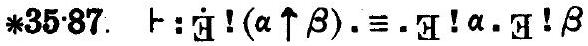
\includegraphics[max width=\textwidth, alt={}, center]{bc1848bf-39e8-4760-b069-9936044df683-148_46_588_1543_209}\\
Dem．

$$
\begin{aligned}
& \text { ト.*35-103.つ : : 写! }(\alpha \uparrow \beta) . \equiv:\left(H^{x}, y\right) . x \in \alpha . y \in \beta: \\
& \text { [*1154] } \equiv:(\mathrm{H} x) . x \in \alpha:(\mathrm{H} y) . y \epsilon \beta \text { : } \\
& \text { [*24.5] 三: 近! α.才! β:. ɔ…Prop }
\end{aligned}
$$

＊35．88． $\mathrm{F}: \alpha \uparrow \beta=\dot{\Lambda} . \equiv: \alpha=\Lambda . \mathrm{v} . \beta=\Lambda$\\
［＊35．87 ．Transp ．＊24：51 ．＊25．51］\\
＊35881． ！： $\mathbb{G}^{\prime} R$ C $\alpha . \supset . R \mid(\alpha \uparrow \beta)=\mathrm{D}^{\prime} R \uparrow \beta$\\
Dem．


\begin{align*}
& \vdash \cdot * 34 \cdot 1 \cdot * 35 \cdot 103 \cdot \supset \\
& \vdash: x\{R \mid(\alpha \uparrow \beta)\} y \cdot \equiv \cdot(\mathrm{~Hz}) \cdot x R z \cdot z \in \alpha \cdot y \in \beta \tag{1}
\end{align*}


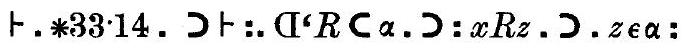
\includegraphics[max width=\textwidth, alt={}, center]{bc1848bf-39e8-4760-b069-9936044df683-149_50_686_205_223}\\
［＊4＇73］


\begin{equation*}
\nu: x R z . \equiv . x R z . z \in \alpha \tag{2}
\end{equation*}


$\vdash .(1) .(2) . \supset \vdash:: \mathrm{Hp} . \supset: x\{R \mid(\alpha \uparrow \beta)\} y . \equiv:(\mathbb{H} z) . x R z . y \epsilon \beta:$\\
［＊10．35］\\
$\equiv:(\mathrm{H} z) . x R z: y \in \beta:$\\
［＊33•13］\\
$\equiv: x \in \mathrm{D}^{\prime} R . y \epsilon \beta$ ：\\
［＊35•103］\\
$\equiv: x\left(\mathrm{D}^{\prime} R \uparrow \beta\right) y::$ ɔ ．Prop\\
＊35．882． $\mathrm{F}: \mathrm{D}^{\prime} R \subset \beta$. J．$(\alpha \uparrow \beta) \mid R=\alpha \uparrow$ T $^{\prime} R$［Similar proof］\\
＊35．89．$\quad \vdash: \mathcal{H}!\beta$ ． ．$(\alpha \uparrow \beta)|(\beta \uparrow \gamma)=(\alpha \uparrow \gamma): \sim G!\beta . \supset .(\alpha \uparrow \beta)|(\beta \uparrow \gamma)=\dot{\Lambda}$\\
Dem．\\
ト.$* 34 \cdot 1$. つ ：.$x\{(\alpha \uparrow \beta) \mid(\beta \uparrow \gamma)\} z$.

\[
\begin{array}{ll} 
& \equiv:(\mathrm{H} y) . x(\alpha \uparrow \beta) y . y(\beta \uparrow \gamma) z: \\
{[* 35 \cdot 103]} & \equiv:(\mathrm{H} y) . x \in \alpha . y \in \beta . y \in \beta . z \in \gamma: \\
{[* 4.24]} & \equiv:(\mathrm{H} y) . x \in \alpha . y \in \beta . z \in \gamma: \\
{[* 10 \cdot 35]} & \equiv: \mathrm{H}!\beta: x \in \alpha . z \in \gamma: \\
{[* 35 \cdot 103]} & \equiv: \mathrm{H}!\beta: x(\alpha \uparrow \gamma) z  \tag{1}\\
\vdash .(1) . \supset \vdash:: \mathrm{H}!\beta . \supset: x\{(\alpha \uparrow \beta) \mid(\beta \uparrow \gamma)\} z . \equiv . x(\alpha \uparrow \gamma) z: \\
& \sim(\mathrm{H}!\beta) . \supset: \sim[x\{(\alpha \uparrow \beta) \mid(\beta \uparrow \gamma)\} z]:: \supset \vdash . \text { Prop }
\end{array}
\]

＊35－891． $\mathrm{F}: \mathcal{H}!\beta . \mathrm{v} . \sim \operatorname{H}!\alpha:$ J．$(\alpha \uparrow \beta)(\beta \uparrow \alpha)=(\alpha \uparrow \alpha)$\\
Dem．\\
ト．＊35．88．ɔ ：： Д ！$\alpha$. ɔ $. \alpha \uparrow \alpha=\dot{\Lambda} . \alpha \uparrow \beta=\dot{\Lambda}$.

\[
\begin{array}{ll}
{[* 34 \cdot 32]} & \supset \cdot \alpha \uparrow \alpha=\dot{\Lambda} \cdot(\alpha \uparrow \beta) \mid(\beta \uparrow \alpha)=\dot{\Lambda} . \\
{[* 21 \cdot 24]} & \supset \cdot(\alpha \uparrow \alpha)=(\alpha \uparrow \beta) \mid(\beta \uparrow \alpha)  \tag{1}\\
\vdash \cdot(1) \cdot * 35 \cdot 89 . \supset \vdash . \text { Prop }
\end{array}
\]

＊35892． $\mathrm{F}:(\alpha \uparrow \alpha)^{2}=(\alpha \uparrow \alpha)$

$$
\left[* 35 \cdot 891 \frac{\alpha}{\beta}\right]
$$

＊35．895． $\mathrm{F}: \alpha \cap \beta=\Lambda . \supset .(\alpha \uparrow \beta)^{2}=\dot{\Lambda} \quad[* 35.68 .82]$\\
＊35．9．$\quad$ F． $\mathrm{D}^{\prime}(\alpha \uparrow \alpha)=\mathbb{G}^{\prime}(\alpha \uparrow \alpha)=C^{\prime}(\alpha \uparrow \alpha)=\alpha$\\
Dem．

\[
\begin{array}{lc}
\vdash \cdot * 358586 . & \supset \vdash: \mathbb{G}!\alpha \cdot \supset \cdot D^{\prime}(\alpha \uparrow \alpha)=\alpha \cdot G^{\prime}(\alpha \uparrow \alpha)=\alpha  \tag{1}\\
\vdash \cdot * 35 \cdot 88, & \supset \vdash: \sim \mathbb{G}!\alpha \cdot \supset \cdot \sim_{H}!(\alpha \uparrow \alpha) . \\
{[* 33 \cdot 29]} & \supset . D^{\prime}(\alpha \uparrow \alpha)=\Lambda . G^{\prime}(\alpha \uparrow \alpha)=\Lambda . \\
{[* 24 \cdot 51]} & \supset . D^{\prime}(\alpha \uparrow \alpha)=\alpha . G^{\prime}(\alpha \uparrow \alpha)=\alpha(2) \\
\vdash .(1) \cdot(2) \cdot * 4 \cdot 83 . \supset \vdash . D^{\prime}(\alpha \uparrow \alpha)=G^{\prime}(\alpha \uparrow \alpha)=\alpha . \supset \vdash . \text { Prop }
\end{array}
\]

＊35．91．$\vdash: R$ C $\alpha \uparrow \alpha . \equiv . C^{6} R \mathrm{C} \alpha$\\
Dem．

$$
\begin{aligned}
\vdash \cdot * 35 \cdot 103 . \text { ว। }: R \text { C } \alpha \uparrow \alpha . & \equiv: x R y . \supset_{x, y} . x, y \in \alpha: \\
& \equiv: C^{6} R \subset \alpha: . \text { J+. Prop } \\
{[* 33 \cdot 352] } &
\end{aligned}
$$

＊35．92．$\vdash: .\left(\mathrm{H}^{\alpha}\right) . P=\alpha \uparrow \alpha . \supset: R \subset P . \equiv . C^{6} R \subset C^{6} P[* 35991]$\\
*35.93. $\quad \vdash:(R) \cdot \phi\left(\mathrm{D}^{\prime} R\right) \cdot \equiv \cdot(\alpha) \cdot \phi \alpha$\\
Dem.

\[
\begin{array}{ll}
\vdash \cdot * 33 \cdot 12 \cdot * 14 \cdot 18 . & \supset \vdash:(\alpha) \cdot \phi \alpha \cdot \supset \cdot \phi\left(\mathrm{D}^{\prime} R\right): \\
{[* 10 \cdot 11 \cdot 21]} & \supset \vdash:(\alpha) \cdot \phi \alpha \cdot \supset \cdot(R) \cdot \phi\left(\mathrm{D}^{\prime} R\right) \\
\vdash \cdot * 10 \cdot 1 . & \supset \vdash:(R) \cdot \phi\left(\mathrm{D}^{\prime} R\right) \cdot \supset \cdot \phi\left\{\mathrm{D}^{\prime}(\alpha \uparrow \alpha)\right\} . \\
{[* 35 \cdot 9]} & \supset \cdot \phi \alpha: \\
{[* 10 \cdot 11 \cdot 21]} & \supset \vdash:(R) \cdot \phi\left(\mathrm{D}^{\prime} R\right) \cdot \supset \cdot(\alpha) \cdot \phi \alpha  \tag{2}\\
\vdash \cdot(1) \cdot(2) . & \supset \vdash \cdot \operatorname{Prop}
\end{array}
\]

*35.931. $\vdash:(R) \cdot \phi\left(\mathrm{G}^{4} R\right) \cdot \equiv \cdot(\alpha) \cdot \phi \alpha \quad$ [Proof as in *35.93]\\
*35.932. $+:(R) \cdot \phi\left(C^{\prime} R\right) \cdot \equiv \cdot(\alpha) \cdot \phi \alpha \quad$ [Proof as in *35.93]\\
*35.94. $\quad \mathrm{F}:(\mathrm{H} R) \cdot \phi\left(\mathrm{D}^{4} R\right) \cdot \equiv \cdot(\mathrm{H} \alpha) \cdot \phi \alpha \quad$ [*35.93. Transp]\\
*35.941. $\mathrm{F}:(\mathrm{H} R) \cdot \phi\left(\mathrm{G}^{c} R\right) \cdot \equiv \cdot\left(\mathrm{H}^{\alpha}\right) \cdot \phi \alpha$ [*35.931. Transp]\\
*35.942. $\mathrm{F}:(\mathrm{H} R) \cdot \phi\left(C^{6} R\right) \cdot \equiv \cdot\left(\mathrm{H}^{\alpha}\right) \cdot \phi \alpha \quad$ [*35.932. Transp]

\section*{＊36．RELATIONS WITH LIMITED FIELDS}
\section*{Summary of＊36．}
In this number we are concerned with the special case in which the same limitation is imposed upon the domain and the converse domain of a relation． In this case，the same result is achieved by imposing the limitation on the field．It is convenient to be able to regard $\alpha \upharpoonleft P\lceil\alpha$ as a descriptive function of $\alpha$ or of $P$ ，which we secure by the notation $P[\alpha$ ，whence，as will be ex－ plained in＊38，$P$ ！$^{\prime} \alpha$ and ↓ $\alpha^{\prime} P$ will both mean $P$ ！$\alpha$ ．If $P$ is a serial relation， and $\alpha \subset C^{4} P$ ，＂$P$ ↓ $\alpha$＂will stand for＂the terms of $\alpha$ arranged in the order determined by $P$ ，＂or，as we may call it briefly；＂$\alpha$ in the $P$－order．＂$P[\alpha$ is defined as follows：\\
＊36．01．$P\lceil\alpha=\alpha \uparrow P \uparrow \alpha \quad$ Df\\
We thus have\\
＊36：13．$\vdash: x(P$ ᄃ $\alpha) y . \equiv . x, y \in \alpha . x P y$\\
Most of the propositions concerning $P\lceil\alpha$ demand that $P$ should have some at least of the characteristics of a serial relation．Hence the propositions concerning $P$ ↓ $\alpha$ which can be given in the present number are，for the most part，not the most useful propositions concerning $P[\alpha$ ．The most useful propositions in the present number are the following：\\
＊36．25．$\vdash: C^{6} P \subset a . \equiv . P\lceil\alpha=P$\\
＊36．29． ト．$P\lceil\alpha=P$ ก $\alpha \uparrow \alpha$\\
＊363．ト．$P\left\lceil\alpha=P!\left(\alpha \cap C^{6} P\right)\right.$\\
＊3633． ト．$P\left[C^{6} P=P\right.$\\
＊36．01．$P\lceil\alpha=\alpha\rceil P\lceil\alpha$ Df\\
＊36．11．$\vdash . P[\alpha=\alpha 1 P \uparrow \alpha \quad[(* 36.01)]$\\
＊36．13．$F: x(P$［ $\alpha) y . \equiv . x, y \in \alpha . x P y \quad[* 36 \cdot 11 . * 35 \cdot 102]$\\
The following propositions are obtained from those of $* 35$ by means of ＊36．11，which，as it is used in each case，is not referred to again．\\
＊36．2．$\quad$ ト．$P$［ $\alpha \dot{\circ} Q \_\beta=(P \dot{\circ} Q)$［ $(\alpha \cap \beta) \quad[* 35 \cdot 15]$\\
＊36201． ト.$P$ ！$\alpha \dot{\cap} P$ ！$\beta=P[(\alpha \cap \beta) \quad[* 36 \cdot 2]$\\
＊36．202． ト．$P$［ $\alpha \dot{\cap} Q\lceil\alpha=(P \dot{\cap} Q)\lceil\alpha \quad[* 36.2]$\\
＊36．203． ト．$P$［ $\alpha \dot{\cap} Q=(P \dot{\cap} Q)$［ $\alpha$［＊35．18］\\
＊36．21． ト．$(P$［ $\alpha)$［ $\beta=P$［ $(\alpha \cap \beta) \quad[* 35 \cdot 33 \cdot 34]$\\
＊36．22．$\quad$ ㄱ．$(P$ ㄷ $\alpha) \mid(Q$ ᄃ $\alpha) \in(P \mid Q)$ ᄃ $\alpha$\\
Dem．\\
$\vdash . * 36 \cdot 13 . * 34 \cdot 1 . \supset \vdash: x\{(P \downharpoonright \alpha) \mid(Q\lceil\alpha)\} z . \equiv .(\mathrm{H} y) . x, y, z \in \alpha . x P y . y Q z$.\\
［＊10：5］


\begin{equation*}
\text { ɔ } \cdot(\text { }(\text { H } y) \cdot x, z \in \alpha \cdot x P y \cdot y Q z \tag{1}
\end{equation*}


ト．（1）．＊1035．＊341． 3 ト．Prop\\
＊36．23．$\quad$ F．$(P \cup Q)[\alpha=P[\alpha \cup Q[\alpha \quad[* 35 \cdot 422]$\\
＊36．24．$\quad \vdash: \alpha \subset \beta$. ɔ．$P$［ $\alpha \in P$［ $\beta \quad$［＊35．432］\\
＊36．241．$\vdash: P \in Q$. J．$P$［ $\alpha \in Q$［ $\alpha \quad$［＊35．462］\\
＊3625． । $: C^{6} P$ C $\alpha . \equiv . P\lceil\alpha=P$\\
Dem．

$$
\begin{aligned}
\vdash \cdot * 36 \cdot 13 \cdot * 4 \cdot 7 \cdot \supset \vdash: P[\alpha=P & \equiv: x P y \cdot \supset_{x, y} \cdot x, y \in \alpha: \\
{[* 33 \cdot 352] } & \equiv: C^{6} P \subset \alpha: . \supset \vdash . \text { Prop }
\end{aligned}
$$

＊36．26．$\quad \vdash: C^{\prime} P \cap \alpha=\Lambda$. J．$P\left(Q \_\alpha\right)=\dot{\Lambda} .\left(Q \_\alpha\right) \mid P=\dot{\Lambda} \quad[* 35 \cdot 473 \cdot 474]$\\
＊3627．\\
＋$: P[\Lambda=\dot{\Lambda} \quad[* 35 \cdot 75]$\\
＊36．28． F．$P[\mathrm{~V}=P$［＊35．76］\\
＊36．29．ト．$P[\alpha=P \dot{n} \alpha \uparrow \alpha$［＊35．822］\\
＊363．$\quad$ ト．$P \backslash \alpha=P \complement\left(\alpha \cap C^{6} P\right)$\\
Dem．\\
ト．$* 33 \cdot 17 \cdot * 4 \cdot 71$. つ $: x P y . \equiv . x, y \in C^{6} P . x P y:$\\
［Fact］$\quad \supset \mathrm{F}: x, y \in \alpha . x P y . \equiv . x, y \in \alpha . x, y \in C^{6} P . x P y$ ．\\
［＊22•33］ $\equiv . x, y \in \alpha \cap C^{6} P . x P y$.\\
［＊36．13］ $\equiv . x\left\{P\left[\left(\alpha \cap C^{6} P\right)\right\} y\right.$

ト．（1）．＊36．13．ɔ. Prop\\
＊3631．$F: \alpha \cap C^{\prime} P=\Lambda$. つ．$P[\alpha=\dot{\Lambda} \quad[* 36.3 \cdot 27]$\\
＊36．32．$F: \alpha \cap C^{\prime} P=\beta \cap C^{\prime} P$. J．$P$ s $\alpha=P[\beta \quad[* 36.3]$\\
＊3633． ト．$P\left[C^{6} P=P\right.$［＊3625］\\
＊36．34．F． $\mathrm{Cnv}^{4} P[\alpha=(\breve{P})[\alpha$［＊35．53］\\
＊3635．$F .\left(P[\alpha)^{2} \subset\left(P^{2}\right)[\alpha\right.$［＊3622］\\
＊364．F：$\alpha \cap D^{\prime} R=\Lambda . \mathrm{v} . \alpha \cap \mathbb{G}^{\prime} R=\Lambda: \supset .(R \cup S)[\alpha=S$ ↓ $\alpha$\\
Dem．\\
ト．＊35．643．ɔ ：$\alpha \cap \mathrm{D}^{\prime} R=\Lambda . \supset . \alpha \dagger(R \cup S)=\alpha \upharpoonleft S$.\\
［＊35．21］$\quad \supset .(R \cup S)[\alpha=S[\alpha$

Similarly $\quad F: \alpha \cap \mathbb{I}^{\prime} R=\Lambda . \supset .(R \cup S)[\alpha=S[\alpha$

ト．（1）．（2）．ɔ. Prop

\section*{*37. PLURAL DESCRIPTIVE FUNCTIONS}
\section*{Summary of *37.}
In this number, we introduce what may be regarded as the plural of $R^{\prime} y$. " $R^{\prime} y$ " was defined to mean "the term which has the relation $R$ to $y$." We now introduce the notation " $R$ " $\beta$ " to mean "the terms which have the relation $R$ to members of $\beta$." Thus if $\beta$ is the class of great men, and $R$ is the relation of wife to husband, $R$ " $\beta$ will mean "wives of great men." If $\beta$ is the class of fractions of the form $1-1 / 2^{n}$ for integral values of $n$, and $R$ is the relation "less than," $R$ " $\beta$ will be the class of fractions each of which is less than some member of this class of fractions, i.e. $R$ " $\beta$ will be the class of proper fractions. Generally, $R^{\text {" }} \beta$ is the class of those referents which have relata that are members of $\beta$.

We require also a notation for the relation of $R$ " $\beta$ to $\beta$. This relation we will call $R_{\mathrm{e}}$. Thus $R_{\mathrm{e}}$ is the relation which holds between two classes $\alpha$ and $\beta$ when $\alpha$ consists of all terms which have the relation $R$ to some member of $\beta$.

A specially important case arises when $R^{6} y$ always exists if $y \in \beta$. In this case, $R^{\prime \prime} \beta$ is the class of all terms of the form $R^{6} y$ when $y \in \beta$. We will denote the hypothesis that $R^{6} y$ always exists if $y \in \beta$ by the notation E !! $R^{\prime \prime} \beta$, meaning "the $R$ 's of $\beta$ 's exist."

The definitions are as follows:


\begin{equation*}
R " \beta=\widehat{x}\{(\text { H } y) \cdot y \epsilon \beta \cdot x R y\} \quad \text { Df } \tag{$* 37.01$.}
\end{equation*}


*37.02.

$$
R_{\varepsilon}=\hat{\alpha} \hat{\beta}\left(\alpha=R^{\prime \prime} \beta\right) \quad \text { Df }
$$

*37.03.

$$
\breve{R}_{\mathrm{e}}=\operatorname{Cnv} v^{\prime}\left(R_{e}\right)
$$

Df\\
This definition serves merely for the avoidance of brackets. Without it, " $\breve{R_{\epsilon}}$ " would be ambiguous as between $(\breve{R})_{\epsilon}$ and $\operatorname{Cnv}^{\prime}\left(R_{\epsilon}\right)$, which are not equal. In all cases in which a suffix occurs, we shall adopt the same convention, i.e. we shall always put

$$
\breve{R}_{\text {suffix }}=\operatorname{Cnv}^{\prime}\left(R_{\text {suffix }}\right) .
$$


\begin{equation*}
R^{\prime \prime \prime} \kappa=R_{e}{ }^{\prime \prime} \kappa \quad \text { Df } \tag{$* 37.04$.}
\end{equation*}


Thus $R$ " $\kappa$ consists of all classes which have the relation $R_{e}$ to some member of $\kappa$. $R$ " $\kappa$ is only significant when $\kappa$ is a class of classes relatively to members of the converse domain of $R$; in this case, $R^{\text {" }}$ " $\kappa$ is a class of classes relatively to members of the domain of $R$.

\section*{*37.05. E!! $R^{\prime \prime} \beta .=: y \in \beta . \nu_{y} . \mathrm{E}!R^{\prime} y \quad$ Df}
Here the symbol " $\mathrm{E}!!R^{\prime \prime} \beta$ " must be treated as a whole, i.e. we must not regard it as making an assertion about $R^{\prime \prime} \beta$. If $R^{\prime \prime} \beta=\alpha$, we must not suppose\\
that we shall be able to put " $E$ ! $\alpha$," which would be nonsense, just as " $E$ ! $x$ " is nonsense even when $x=R^{6} y$ and $\mathrm{E}!R^{6} y$.

The notation $R$ " $\alpha$, introduced in the present number, is extremely useful, and embodies a very important idea. Its use is somewhat different according to the kind of relation concerned. Consider first the kind of relation which leads to a descriptive function, say $D$. If $\lambda$ is a class of relations, $D$ " $\lambda$ is the class of the domains of these relations. In this case, $\mathrm{D}^{\prime \prime} \lambda$ is a class each of whose members is of the form $\mathrm{D}^{\prime} R$, where $R \in \lambda$. Again, let us denote by " $\times n$ " the relation of $m$ to $m \times n$; then if we denote by " $N C$ " the class or cardinal numbers, $\times n^{\text {" }} N C$ will denote all numbers that result from multiplying a cardinal number by $n$, i.e. all multiples of $n$. Thus e.g. $\times 2$ " $N C$ will be the class of even numbers. If $R$ is a correlation between two classes $\alpha$ and $\beta$, i.e. a relation such that, if $y \in \beta, R^{\prime} y$ exists and is a member of $\alpha$, while conversely, if $x \in \alpha, \breve{R}^{\prime} x$ exists and is a member of $\beta$, then $\alpha=R^{\prime \prime} \beta$, and we may regard $R$ as a transformation applied to each member of $\beta$ and giving rise to a member of $\alpha$. It is by means of such transformations that two classes are shown to be similar, i.e. to have the same (cardinal) number of terms.

In the case of serial relations, the utility of the notation $R$ " $\beta$ is somewhat different. Suppose, for example, that $R$ is the relation of less to greater among real numbers. Then if $\beta$ is any class of real numbers, $R$ " $\beta$ will be the segment of real numbers determined by $\beta$, i.e. the class of real numbers which are less than the limit or maximum of $\beta$. In any series, if $\beta$ is a class contained in the series and $R$ is the generating relation of the series, $R^{\prime \prime} \beta$ is the segment determined by $\beta$. If $\beta$ has either a limit or a maximum, say $x, R^{\prime \prime} \beta$ will be $\vec{R}^{\prime} x$. But if $\beta$ has neither a limit nor a maximum, $R^{\prime \prime} \beta$ will be what we may call an "irrational" segment of the series. We shall see at a later stage that the real numbers may be identified with the segments of the series of rationals, i.e. if $R$ is the relation of less to greater among rationals, the real numbers will be all classes such as $R^{\prime \prime} \beta$, for different values of $\beta$. The real numbers which correspond to rationals will be those resulting from a $\beta$ which has a limit or maximum; the irrationals will be those resulting from a $\beta$ which has no limit or maximum.

The present number may be divided into various sections, as follows: (1) First, we have various elementary properties of the terms defined at the beginning of the number; this section ends with $* 3729$. (2) We have next a set of propositions dealing with relative products, and with such symbols as $P$ " $Q$ " $\gamma, P^{\prime \prime} Q$ " $\kappa$, and so on. The central proposition here is\\
*37:33. ト $.(P \mid Q)^{6 \prime} \gamma=P$ " $Q$ " $\gamma$\\
By the definition, $Q$ " $\kappa=Q_{\epsilon}$ " $\kappa$. Thus $P$ " $Q$ " $\kappa=\left(P \mid Q_{\epsilon}\right)$ " $\kappa$. This connects propositions concerning such symbols as $P$ " $Q$ " $\kappa$ with propositions concerning\\
relative products．This second section consists of the propositions from＊37．3 to＊37：39．（3）We have next a set of propositions on relations with limited domains and converse domains．The chief of these are\\
＊37：401．ト． $\mathrm{D}^{c}(R \uparrow \beta)=R$＂$\beta$\\
＊37 412． ト $.(R \uparrow \alpha)^{c} \beta=R^{c \prime}(\alpha \cap \beta)$\\
＊3741．＋． $\mathrm{D}^{\prime}\left(R[\alpha)=\alpha \cap R\right.$＂$\alpha . \mathrm{G}^{\prime}(R[\alpha)=\alpha \cap \breve{R}$＂$\alpha$\\
These propositions on relations with limited domains and converse domains， together with certain others naturally connected with them，extend from $* 37 \cdot 4$ to $* 37.52$ ．（4）We next have a number of very important propositions on the consequences of the hypothesis $\mathrm{E}!!R$＂$\beta$ ，i．e．the hypothesis that，for any argument which is a member of $\beta, R$ gives rise to a descriptive function $R^{6} y$ ． The chief proposition in this section is\\
＊37．6．$\quad$ t： $\mathrm{E} \|$ ！$R^{\prime \prime} \beta$ ．ɔ ．$R^{\prime \prime} \beta=\widehat{x}\left\{(\right.$ H $\left.y) \cdot y \in \beta \cdot x=R^{\prime} y\right\}$\\
Propositions with the hypothesis $\mathrm{E}!!R$＂$\beta$ are applied to the cases of $\vec{R}$ and $\overleftarrow{R}$ ，in which the hypothesis is verified．This section extends from＊37．6 to $* 37 \cdot 791$ ．（5）Finally，we have three propositions on the relative product of $\alpha \uparrow \beta$ with other relations．These propositions are useful in relation－ arithmetic（Part IV）．

The propositions of the present number which are most used in the sequel， apart from those already mentioned，are the following（omitting such as merely embody definitions）：\\
＊3715．$\quad$ ․ $R$＂$\alpha$ CD＇$R$\\
＊37－16．＋．$\breve{R}^{\prime \prime} \alpha \subset$ C＇$R$\\
＊372．$\quad$ ：$\alpha \subset \beta$ ．ɔ ．$P$＂$\alpha \subset P$＂$\beta$\\
＊37．22． ト．$P$＂$(\alpha \cup \beta)=P$＂$\alpha \cup P$＂$\beta$\\
＊37：25．ㅏ． $\mathrm{D}^{\prime} R=R^{\prime \prime} \mathrm{G}^{\prime} R . \mathrm{G}^{\prime} R=\breve{R}^{\prime \prime} \mathrm{D}^{\prime} R$\\
＊37：26． ナ．$R^{\prime \prime} \beta=R^{\prime \prime}\left(\beta \cap \mathbb{C}^{\prime} R\right)$\\
＊37265． ト $. R^{\prime \prime} \alpha=R^{\prime \prime}\left(\alpha \cap C^{\prime} R\right) . \breve{R}^{\prime \prime} \alpha=\breve{R}$＂$\left(\alpha \cap C^{\prime} R\right)$\\
＊3729． ト $. R^{\prime \prime} \Lambda=\Lambda . \breve{R}^{\prime \prime} \Lambda=\Lambda$\\
＊3732．F． $\mathrm{D}^{\prime}(P \mid Q)=P$＂D＇$Q . \mathrm{G}^{\prime}(P \mid Q)=\breve{Q}$＂Q＇$P$\\
＊3745． ト：．$(y)$ ．E $!R^{\prime} y$ ． J：H！$R^{\prime \prime} \beta$ ．三 ． H！$\beta$\\
＊3746．$\vdash: x \in R$＂$\alpha . \equiv$ ． 田！$\alpha \cap \overleftarrow{R^{\prime}} x$\\
＊3761．$+:: \mathrm{E}!!R^{\prime \prime} \beta . \supset: R^{\prime \prime} \beta \subset \alpha . \equiv: y \in \beta . \supset_{y} . R^{\prime} y \in \alpha$\\
For example，let $R$ be the relation of father to son，$\beta$ the class of Etonians， $\alpha$ the class of rich men；then＂$R$＂$\beta \subset \alpha$＂states＂all fathers of Etonians are rich，＂while＂$y \in \beta . \partial_{y} . R^{6} y \in \alpha$＂states＂if a boy is an Etonian，his father\\
must be rich．＂In virtue of the above proposition，these two statements are equivalent．\\
＊3762．$\vdash: \mathrm{E}!R^{\prime} y, y \in \alpha$. つ.$R^{\prime} y \in R^{\prime \prime} \alpha$\\
＊37．63．$\vdash:: \mathrm{E}!!R^{\prime \prime} \alpha . \supset: . x \in R^{\prime \prime} \alpha . \partial_{x} \cdot \psi x: \equiv: y \in \alpha . \partial_{y} \cdot \psi\left(R^{\prime} y\right)$\\
＊37．01．$R^{\prime \prime} \beta=\widehat{x}\{(\mathrm{H} y) \cdot y \in \beta \cdot x R y\} \quad$ Df\\
＊37．02．$R_{\epsilon}=\hat{\alpha} \hat{\beta}(\alpha=R " \beta) \quad$ Df\\
＊37．03．$\breve{R}_{\epsilon}=\operatorname{Cnv}^{\prime}\left(R_{e}\right) \quad$ Df\\
＊37．04．$R^{c "} \kappa=R_{\epsilon}{ }^{c} \kappa$ Df\\
＊37．05．E！！$R^{\prime \prime} \beta .=: y \in \beta . \partial_{y} . \mathrm{E}!R^{\prime} y$ Df\\
$* 371 . \quad \vdash: x \in R R^{\prime \prime} \beta . \equiv .(\mathrm{H} y) . y \in \beta . x R y \quad[* 203 .(* 37 \cdot 01)]$\\
＊37．101．$+: \alpha R_{e} \beta . \equiv \alpha=R^{\prime \prime} \beta$［＊213．（＊37．02）］\\
＊37－102．$\vdash: \alpha(\breve{R})_{\epsilon} \beta . \equiv . \alpha=\breve{R}$＂$\beta$［＊37•101］\\
＊37－103．$f: \alpha \in R^{\prime \prime \prime} \kappa . \equiv .(\mathrm{H} \beta) . \beta \in \kappa . \alpha=R^{\prime \prime} \beta . \equiv . \alpha \in R_{\epsilon}$＂$\kappa [* 37 \cdot 1 \cdot 101 .(* 37 \cdot 04)]$\\
＊37－104．$+: . \mathrm{E}!!R^{\prime \prime} \beta . \equiv: y \in \beta . \supset_{y} . \mathrm{E}!R^{\prime} y \quad[* 4 \cdot 2 .(* 37 \cdot 05)]$\\
＊37－105．$+: x \in \breve{R}$＂$\beta . \equiv .($ H $y) . y \in \beta . y R x \quad$［＊37．1．＊31．11］\\
＊37－106． ↓ ： $\mathrm{E}!R^{6} x . \supset: x \in \breve{R}^{\prime \prime} \beta . \equiv R^{\prime} x \in \beta$\\
Dem．

$$
\begin{aligned}
& \vdash \cdot * 37 \cdot 105 \cdot * 30 \cdot 4 \cdot \supset \vdash: \mathrm{Hp} \cdot \supset: x \in \breve{R^{\prime \prime}} \beta . \equiv(\text { H } y) \cdot y \in \beta \cdot y=R^{\prime} x . \\
& {[* 14 \cdot 205]} \\
& \quad \equiv R^{\prime} x \in \beta: . \supset \vdash . \text { Prop }
\end{aligned}
$$

＊37－11． ト．$R_{\mathrm{e}}{ }^{\prime} \beta=R^{\prime \prime} \beta$ ［＊37•101．＊30：3］\\
＊37－111． $\mathrm{F} . \mathrm{E}!R_{\mathrm{e}}{ }^{6} \beta$［＊37•11．＊14•21］\\
＊37．12． $\mathrm{F}:(\beta) \cdot R^{\prime \prime} \beta=Q^{\prime} \beta \cdot \equiv \cdot R_{\epsilon}=Q \quad[* 30 \cdot 42 \cdot * 37 \cdot 111 \cdot 11]$\\
＊37．13． F $: P=Q . \supset . P " \beta=Q " \beta$\\
Dem．\\
ト．＊21．43．ɔ $: . \mathrm{Hp} . \supset: x P y . \equiv_{x, y} . x Q y:$\\
［Fact］$\quad J: y \in \beta . x P y . \equiv_{x, y}, y \in \beta . x Q y:$\\
［＊10281］$\quad$ ：（H $y) . y \in \beta . x P y . \equiv_{x} .($ H $y) . y \in \beta . x Q y$ ：\\
［＊37．1］$\quad \supset: x \in P$＂$\beta . \equiv_{x} . x \in Q$＂$\beta$ ：．ɔ ．Prop\\
＊37：131．$\vdash: P=Q$. J．$P_{\epsilon}=Q_{\epsilon}$\\
Dem．

$$
\begin{aligned}
& \vdash \cdot * 37 \cdot 13 . \supset \vdash: \text { Hp } . \supset: \alpha=P " \beta . \equiv_{\alpha, \beta} \cdot \alpha=Q^{" \beta}: \\
& {[* 37 \cdot 101] \quad \supset: \alpha P_{\epsilon} \beta . \equiv_{\alpha, \beta} \cdot \alpha Q_{\epsilon} \beta: . \supset \text { V. Prop }}
\end{aligned}
$$

＊37．14．$\vdash: P=Q . \equiv . P_{\epsilon}=Q_{\epsilon}$\\
Dem．\\
$\vdash \cdot * 37 \cdot 101 \cdot * 21 \cdot 15 \cdot \nu$\\
$\vdash: P_{\epsilon}=Q_{\epsilon} \cdot \equiv: \alpha=P \backsim \beta . \equiv_{\alpha, \beta} \cdot \alpha=Q \times \beta:$\\
［＊13＇183］$\equiv:(\beta) . P^{\prime \prime} \beta=Q^{\prime \prime} \beta$ ：\\
$[* 37 \cdot 1 \cdot * 20 \cdot 15] \equiv:(\beta, x):(\mathrm{H} y) \cdot y \in \beta, x P y \cdot \equiv \cdot(\mathrm{H} y) \cdot y \in \beta . x Q y:$\\
［＊10．1］$\quad$ ：$(x):($ J $y) \cdot y \in \hat{z}(z=w) \cdot x P y \cdot \equiv$ ．（马 $y) \cdot y \in \hat{z}(z=w) \cdot x Q y$ ：\\
［＊20．3］$\quad$ ：$(x):($ H $y) \cdot y=w \cdot x P y \cdot \equiv \cdot($ H $y) \cdot y=w \cdot x Q y:$\\
［＊13．195］$\quad$ ：$(x): x P w . \equiv . x Q w$

ト．（1）．＊10．11．21．＊11．2．ɔ\\
। ：．$P_{\epsilon}=Q_{\epsilon}$ ．J：$(x, w): x P w . \equiv . x Q w:$\\
［＊21＊43］$\quad \supset: P=Q$

ト．（2）．＊37．131．つ ．Prop\\
＊37－15． ト $R$＂$\alpha$ C D $R$\\
Dem．

$$
\vdash * 37 \cdot 1 . \supset \vdash: x \in R \text { " } \alpha . \supset .(\mathrm{H} y) . y \in \alpha . x R y .
$$

$$
\begin{array}{ll}
{[* 10 \cdot 5]} & \text { J. (马y). } x R y \\
{[* 33 \cdot 13]} & \text { J. } x \in \mathrm{D}^{\prime} R: \supset \vdash . \text { Prop }
\end{array}
$$

＊37－16．$\quad$ ．$\breve{R}{ }^{\prime \prime} \alpha \subset \mathbb{C}{ }^{\prime} R \quad\left[* 37 \cdot 15 \frac{\breve{R}}{R} \cdot * 33 \cdot 2\right]$\\
＊37－17． F $: . R$＂$\beta$ C $\alpha . \equiv: y \in \beta . x R y . D_{x, y} . x \in \alpha$\\
Dem．

$$
\begin{aligned}
\vdash \cdot * 37 \cdot 1 . \supset \vdash: R " \beta \subset \alpha . & \equiv:(H y) \cdot y \in \beta . x R y . \partial_{x} \cdot x \in \alpha: \\
{[* 10 \cdot 23] } & \equiv: y \in \beta . x R y . \partial_{x, y} \cdot x \in \alpha: . \supset \vdash . \text { Prop }
\end{aligned}
$$

$* 37171 .+: . \breve{R}^{\prime \prime} \alpha \subset \beta . \equiv: x \in \alpha . x R y . \partial_{x, y}, y \in \beta$\\
Dem．

$$
\begin{aligned}
\vdash \cdot * 37 \cdot 105 . \supset \vdash: \breve{R}^{\prime \prime} \alpha \subset \beta & \equiv:(\mathbb{H} x) \cdot x \in \alpha \cdot x R y \cdot \nu_{y} \cdot y \in \beta: \\
{[* 10 \cdot 23] } & \equiv: x \in \alpha \cdot x R y \cdot \nu_{x, y} \cdot y \in \beta: \text { J } . \text { Prop }
\end{aligned}
$$

＊37－18．$\quad \vdash: y \in \beta$. つ.$\vec{R}^{\prime} y \subset R^{\prime \prime} \beta$\\
Dem．

$$
\begin{aligned}
& \text { ।. } * 32 \cdot 18 . \text { つ }: . \mathrm{Hp} . \text { ɔ }: x \in \vec{R}^{\prime} y . \text { ɔ } . x R y . y \in \beta . \\
& \text { } \begin{aligned}
\text { コ } . x 37 \cdot 1] & . x \in R^{\prime \prime} \beta: . \text { つ } . \text { Prop }
\end{aligned}
\end{aligned}
$$

＊37－181．$\vdash: x \in \alpha$. つ.$\overleftarrow{R}^{6} x \subset \breve{R}^{6 \prime} \alpha \quad$［Proof as in＊37－18］\\
＊37．2． ト：$\alpha \subset \beta$ ． ɔ.$P$＂$\alpha \subset P$＂$\beta$\\
Dem．\\
$\vdash . * 22 \cdot 1 . \supset \vdash: . H p . \supset: y \in α . \partial_{y} . y \in \beta:$\\
$[* 10 \cdot 31] \quad \supset: y \in \alpha . x P y . \supset_{y} . y \in \beta . x P y:$\\
［＊10．28］$\quad$ ：（马 $y$ ）．$y \in \alpha . x P y . \supset .($ H $y) . y \in \beta . x P y$ ：\\
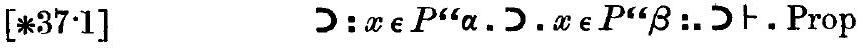
\includegraphics[max width=\textwidth, alt={}, center]{bc1848bf-39e8-4760-b069-9936044df683-157_48_866_2000_263}

The above proposition $(* 37.2)$ is one of the forms of asyllogistic inference due to Leibniz＇s teacher Jungius．The instance given by Jungius is：＂Circulus est figura；ergo qui circulum describit，is figuram describit＊．＂Here the class of circles is our $\alpha$ ，the class of figures is our $\beta$ ，and the relation of describing is our $P$ ．\\
＊37－201． $\mathrm{F}: P \in Q$. J．$P$＂$\alpha \subset Q$＂$\alpha$［Similar proof］\\
＊37．202． $\mathrm{F}: \alpha \subset \beta . P \in Q$. J．$P$＂$\alpha \subset Q$＂$\beta$［＊37．2201］\\
＊37．21．$\quad$ ．$P$＂$(\alpha \cap \beta) \subset P$＂$\alpha \cap P$＂$\beta$\\
Dem．

\begin{verbatim}
ト. $* 37$ 1. J $: . x \in P^{\prime \prime}(\alpha \cap \beta) . \equiv:(\mathrm{H} y) . y \epsilon \alpha \cap \beta . x P y$ :
[*2233] $\equiv:(\mathrm{H} y) . y \in \alpha . y \in \beta . x P y$ :
[*10.5] $\supset:($ H $y) . y \in \alpha . x P y:($ H $y) . y \in \beta . x P y$ :
[*37•1] $\supset: x \in P$ " $\alpha . x \in P$ " $\beta$ :
[*22:33] $\supset: x \in P$ " $\alpha \cap P$ " $\beta:$ : ɔ아. Prop
\end{verbatim}

＊37．211． $\mathrm{F} .(P \dot{\cap} Q)^{c} \alpha \subset P$＂$\alpha \cap Q$＂$\alpha \quad$［Similar proof］\\
＊37－212． F．$(P \dot{\cap} Q)$＂$(\alpha \cap \beta) \subset P$＂$\alpha \cap P$＂$\beta \cap Q$＂$\alpha \cap Q$＂$\beta$［＊37．21•211］\\
＊37：22． ト．$P$＂$(\alpha \cup \beta)=P$＂$\alpha \cup P$＂$\beta$\\
This proposition is very frequently used．The fact that here we have identity，while in $* 37.21$ we only have inclusion，is due to the fact that $* 10.42$ states an equivalence，while $* 10.5$ only states an implication．

Dem．

$$
\begin{array}{ll}
\vdash \cdot * 37 \cdot 1 . \supset \vdash: x \in P "(\alpha \cup \beta) & \equiv:(\text { H } y) \cdot y \in \alpha \cup \beta \cdot x P y: \\
{[* 22 \cdot 34]} & \equiv:(\text { H } y): y \in \alpha \cdot \mathrm{v} \cdot y \in \beta: x P y: \\
{[* 4 \cdot 4]} & \equiv:(\text { H } y): y \in \alpha \cdot x P y \cdot \mathrm{v} \cdot y \in \beta \cdot x P y: \\
{[* 10 \cdot 42]} & \equiv:(\text { H } y) \cdot y \in \alpha \cdot x P y: \mathrm{v}:(\text { H } y) \cdot y \in \beta \cdot x P y: \\
{[* 37 \cdot 1]} & \equiv: x \in P^{\prime \prime} \alpha \cdot \mathrm{v} \cdot x \in P \text { " } \beta: \\
{[* 22 \cdot 34]} & \equiv: x \in P \text { " } \alpha \cup P \text { " } \beta: \text { J } . \text { Prop }
\end{array}
$$

＊37．221．$F .(P \cup Q)$＂$\alpha=P$＂$\alpha \cup Q$＂$\alpha \quad$［Similar proof］\\
＊37．222． F.$(P \cup Q)$＂$(\alpha \cup \beta)=P$＂$\alpha \cup P$＂$\beta \cup Q$＂$\alpha \cup Q$＂$\beta \quad[* 37 \cdot 22 \cdot 221]$\\
＊37．23． $\mathrm{F} . \mathrm{D}{ }^{\prime} R_{\mathrm{e}}=\hat{\alpha}\left\{(\mathrm{H} \beta) . \alpha=R^{\prime \prime} \beta\right\}$［＊37．101．＊33•11］\\
＊37：231． ト ． $\mathrm{U}{ }^{6} R_{\mathrm{e}}=\mathrm{Cls}$\\
The type of＂Cls＂here is that type whose members are of the same type as $G^{\prime} R$ ．In the proof，use is made of the convention that a Greek letter always stands for an expression of the form $\hat{z}(\phi!z)$ ．

Dem．

\[
\begin{array}{ll}
\vdash \cdot * 37 \cdot 101 & \supset \vdash: \alpha R_{\epsilon} \hat{z}(\phi!z) \cdot \equiv \cdot \alpha=R^{6} \hat{z}(\phi!z): \\
{[* 10 \cdot 11 \cdot 281]} & \supset \vdash:\left(H^{\alpha}\right) \cdot \alpha R_{e} \hat{z}(\phi!z) \cdot \equiv \cdot\left(H^{\alpha}\right) \cdot \alpha=R^{6} \hat{z}(\phi!z): \\
{[* 33 \cdot 131]} & \supset \vdash: \hat{z}(\phi!z) \in \mathbb{G}^{6} R_{e} \cdot \equiv \cdot\left(H^{\alpha}\right) \cdot \alpha=R^{6} \hat{z}(\phi!z) \tag{1}
\end{array}
\]

＊We quote from Couturat，La Logique de Leibniz，Chapter iii，§ 15 （p． 75 n．）．

\[
\begin{array}{ll}
\vdash \cdot * 20 \cdot 2 \cdot(* 37 \cdot 01) \cdot \supset \vdash: \hat{x}\{(\mathrm{H} y) \cdot y \in \hat{z}(\phi!z) \cdot x R y\}=R^{6} \hat{z}(\phi!z): \\
{[* 10 \cdot 11 \cdot 24]} & \supset \vdash:(\phi):\left(\mathrm{H}^{\alpha}\right) \cdot \alpha=R^{6} \hat{z}(\phi!z) \\
\vdash \cdot(1) \cdot(2) \cdot * 2 \cdot 02 \cdot & \supset \vdash: \hat{z}(\phi!z) \in \mathrm{Cls} \cdot \supset \cdot \hat{z}(\phi!z) \in \mathrm{G}^{6} R_{e} \\
\vdash \cdot * 20 \cdot 41 \cdot * 2 \cdot 02 . & \supset \vdash: \hat{z}(\phi!z) \in \mathrm{G}^{6} R_{e} \cdot \supset \cdot \hat{z}(\phi!z) \in \mathrm{Cls}  \tag{4}\\
\vdash \cdot(3) \cdot(4) . & \supset \vdash . \text { Prop }
\end{array}
\]

As appears in the above proof，it is necessary，when a proposition con－ taining＂Cls＂is to be proved，to abandon the notation with Greek letters，and revert to the explicit functional notation．\\
＊37．24．$\quad \mathrm{F}: \alpha \in \mathrm{D}^{\prime} R_{.}$． J．$\alpha \subset \mathrm{D}^{\prime} R$\\
Dem．

$$
\begin{aligned}
& \text { ト } \cdot * 33 \cdot 13 \cdot * 37 \cdot 101 . \text { つ } \vdash:: \alpha \in \mathrm{D}^{\prime} R_{e} \cdot \equiv:(\text { H } \beta) . \alpha=R^{\prime \prime} \beta: . \\
& {[* 2033 . * 37 \cdot 1] \quad \equiv: \text { (J } \beta \text { ) : } x \in \alpha . \equiv_{x} \cdot(\text { H } y), y \in \beta . x R y \text { : }} \\
& \text { [*1161] } \quad \supset: x \in \alpha . \partial_{x}:(\mathcal{H} \beta, y) . y \in \beta . x R y: \\
& \text { [*1123] } \nu_{x}:(\text { T } y, \beta) . y \in \beta . x R y \text { : } \\
& \text { [*1155] } \quad \nu_{x}:(\mathrm{H} y): x R y:(\mathrm{H} \beta) \cdot y \in \beta: \\
& \text { [*10.5] } \nu_{x}:(\text { H } y) . x R y \text { : } \\
& \text { [*33.13] } \nu_{x}: x \in \mathrm{D}^{6} R:: \supset \vdash \text {. Prop }
\end{aligned}
$$

＊37．25．$\quad$ ‥D ${ }^{\wedge} R=R^{\wedge} \mathbb{Q}^{\wedge} R . \mathbb{G}^{\wedge} R=\breve{R}^{\wedge} \mathrm{D}^{\wedge} R$\\
Dem．


\begin{align*}
& \text { ト.*33-13. ɔト: } x \in \mathrm{D}^{\prime} R \text {. } \equiv \text {. (月 } y \text { ). } x R y \text {. } \\
& \text { [*33.14.**71] } \quad \equiv \text { (J } y \text { ). } y \in \mathbb{C} \text { ⋅ } R . x R y \text {. } \\
& \text { [*37•1] } \equiv . x \in R^{\prime \prime} \mathbb{C}^{\prime} R  \tag{1}\\
& \text { ৮.*33-131. ɔ : } y \in \mathbb{G}^{\prime} R . \equiv .(\mathbb{T} x) . x R y \text {. } \\
& {[* 33 \cdot 14 \cdot * 4 \cdot 71] \quad \equiv \cdot\left(\mathrm{H}^{\mathrm{x}}\right) \cdot x \in \mathrm{D}^{\prime} R . x R y \text {. }} \\
& \text { [*37:105] } \quad \equiv . y \in \breve{R} \text { ‘‘D‘ } R  \tag{2}\\
& \text { ト.(1).(2). ɔㄴ. Prop }
\end{align*}


＊37：26．$\quad$ ．$R^{\prime \prime} \beta=R^{\prime \prime}\left(\beta \cap \mathbb{G}^{\prime} R\right)$\\
Dem．

$$
\begin{array}{ll}
\vdash \cdot * 37 \cdot 1 \cdot \supset \vdash: x \in R^{\prime \prime} \beta . & \equiv:(\mathrm{H} y) \cdot y \in \beta \cdot x R y: \\
{[* 33 \cdot 14 \cdot * 4 \cdot 71]} & \equiv:(\mathrm{G} y) \cdot y \in \beta \cdot y \in \mathrm{G}^{\prime} R . x R y: \\
{[* 22 \cdot 33]} & \equiv:(\mathrm{G} y) \cdot y \in \beta \cap \mathrm{G}^{\prime} R . x R y: \\
{[* 37 \cdot 1]} & \equiv: x \in R^{\prime \prime}\left(\beta \cap \mathrm{G}^{\prime} R\right): . \text { JF. Prop }
\end{array}
$$

＊37．261．.$+ \breve{R}$＂$\beta=\breve{R}$＂$\left(\beta \cap \mathrm{D}^{\prime} R\right)$［＊37．26．＊33．21］\\
＊37．262． $\mathrm{F}: \alpha \cap \mathbb{G}^{\prime} R=\beta \cap \mathbb{G}^{\prime} R$. J．$R$＂$\alpha=R^{\prime \prime} \beta \quad[* 37 \cdot 26]$\\
＊37．263． $\mathrm{F}: \alpha \cap \mathrm{D}$＂$R=\beta \cap \mathrm{D}$＂$R$ ．১．$\breve{R^{\prime \prime}} \alpha=\breve{R}$＂$\beta$［＊37．261］\\
＊37．264．F：H：αn R＂$\beta . \equiv(\mathrm{H} x, y) . x \in \alpha . y \in \beta . x R y . \equiv . \mathrm{E}!\beta \cap \breve{R}$＂$\alpha$\\
Dem．\\
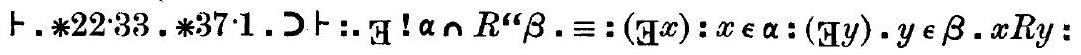
\includegraphics[max width=\textwidth, alt={}, center]{bc1848bf-39e8-4760-b069-9936044df683-159_55_1081_2007_162}


\begin{equation*}
[* 11 \cdot 55] \quad \equiv:\left(\mathrm{H}^{x}, y\right) . x \in \alpha . y \in \beta . x R y \tag{2}
\end{equation*}


ト．（1）．$* 116$. つト：．J！$\alpha \cap R^{\prime \prime} \beta . \equiv:($ 马 $y): y \in \beta:($ G $x) . x \in \alpha . x R y$ ：\\
［＊37•105］


\begin{equation*}
\equiv:(\mathrm{H} y), y \in \beta, y \in \mathrm{R}^{\prime \prime} \alpha: \tag{3}
\end{equation*}


［＊22：33］\\
$\equiv:$ H $!\beta \cap \breve{R}$＂$\alpha$

ト．（2）．（3）．ɔ…Prop\\
＊37－265． ＋$R$＂$\alpha=R$＂$\left(\alpha \cap C^{\prime} R\right) \cdot \breve{R}^{\prime \prime} \alpha=\breve{R}$＂$\left(\alpha \cap C^{\prime} R\right)$\\
Dem．

\[
\begin{array}{ll}
\vdash \cdot * 33 \cdot 161 \cdot * 22 \cdot 621 . & \supset \vdash . G^{6} R=C^{6} R \cap G^{6} R . \\
{[* 22 \cdot 481]} & \supset \vdash . \alpha \cap G^{6} R=\alpha \cap C^{6} R \cap G^{6} R . \\
{[* 37 \cdot 262]} & \supset \vdash . R^{6 \prime} \alpha=R^{6}\left(\alpha \cap C^{6} R\right)  \tag{1}\\
\vdash .(1) . * 33 \cdot 22 . & \supset \vdash . \text { Prop }
\end{array}
\]

＊37．27．$\quad$ ： $\mathbb{C}$ ‘ $R$ C $\beta$ ．ɔ ． $\mathrm{D}^{\prime} R=R^{\prime \prime} \beta \quad[* 22.621 . * 37 \cdot 25 \cdot 26]$\\
＊37．271． $\mathrm{F}: \mathrm{D}^{\prime} R \mathrm{C} \alpha$ ．ɔ． $\mathrm{G} \cdot R=\breve{R}^{\prime \prime} \alpha \quad$［＊22．621．＊37．25．261］\\
＊37－28．$+. R^{\prime \prime} \mathrm{V}=\mathrm{D}^{\prime} R . \breve{R}^{\prime \prime} \mathrm{V}=\mathrm{C}^{\prime} R \quad[* 37 \cdot 27 \cdot 271 . * 24 \cdot 11]$\\
＊3729．$\vdash . R^{\prime \prime} \Lambda=\Lambda . \breve{R}^{\prime \prime} \Lambda=\Lambda$\\
Dem．


\begin{align*}
& \text { ト. } * 105 . \text { つト: }(\text { み } y) . y \epsilon \text { Λ. } x R y . \text { ɔ. }(\text { 马 } y) . y \in \Lambda  \tag{1}\\
& \text { ト.(1).Transp. } * 24 * 53 \text {. ɔ } . \sim(\text { H } y) . y \in \Lambda . x R y \text {. } \\
& \text { [*371] ɔト.~建! } R \text { "Λ. } \\
& \text { [*24:51] ɔト. } R^{\prime \prime} \mathrm{A}=\Lambda  \tag{2}\\
& \text { ト.(2) } \frac{\breve{R}}{R} \text {. } \quad \supset \vdash . \breve{R} \text { " } \Lambda=\Lambda  \tag{3}\\
& \text { ト.(2).(3). ɔ…Prop }
\end{align*}


＊37．3．$\quad \vdash .\left\{\operatorname{sg}^{6}(P \mid Q)\right\}^{6} z=P{ }^{\prime \prime} \vec{Q}^{\prime} z$\\
Dem．

$$
\begin{array}{ll}
\vdash \cdot * 32 \cdot 23 \cdot 13 \cdot \nu & \\
\vdash \cdot\left\{\operatorname{sg}^{6}(P \mid Q)\right\}^{6} z & =\widehat{x}\{x(P \mid Q) z\} \\
{[* 34 \cdot 1]} & =\widehat{x}\{(\text { H } y) \cdot x P y \cdot y(Q z\} \\
{[* 32 \cdot 18]} & =\widehat{x}\left\{(\text { H } y) \cdot x P y \cdot y \in \overrightarrow{Q^{6}} z\right\} \\
{[(* 37 \cdot 01)]} & =P^{6} \vec{Q}^{6} z \cdot \supset+\cdot \text { Prop }
\end{array}
$$

＊37．301．$\vdash .\left\{\text { gs }^{\prime}(P \mid Q)\right\}^{\prime} x=\breve{Q}{ }^{\prime \prime} \overleftarrow{P}_{x} \quad$［Similar proof］\\
＊37302．$\vdash: R=P \mid Q . \supset . \vec{R}^{\prime} z=P{ }^{\prime \prime} \vec{Q}^{\prime} z \cdot \overleftarrow{R}^{\prime} x=\breve{Q}^{\prime \prime} \overleftarrow{P}_{x}$

$$
[* 37 \cdot 3 \cdot 301 \cdot * 32 \cdot 23 \cdot 231 \cdot 16]
$$

＊37．31．$\quad \vdash \cdot \operatorname{sg}^{6}(P \mid Q)=P_{\epsilon} \mid \vec{Q}$\\
Dem．


\begin{align*}
& \vdash \cdot * 37 \cdot 11 \cdot 3 . \quad \text { J } \cdot(z) \cdot\left\{\operatorname{sg}^{6}(P \mid Q)\right\}^{6} z=P_{\epsilon} \vec{Q}^{6} z  \tag{1}\\
& \vdash \cdot(1) \cdot * 34 \cdot 42 . \text { J } \text {. Prop }
\end{align*}


＊37－311． r． $\mathrm{gs}^{\prime}(P \mid Q)=(\breve{Q})_{\epsilon} \mid \overleftarrow{P} \quad$［Similar proof］\\
＊3732．$\quad \vdash . \mathrm{D}^{\prime}(P \mid Q)=P{ }^{\prime \prime} \mathrm{D}^{\prime} Q . \mathrm{G}^{\prime}(P \mid Q)=\breve{Q}^{\prime \prime} \mathrm{G}^{\prime} P$\\
Dem．


\begin{align*}
& \text { ト.*33.13.*34.1.J } \\
& \vdash: . x \in \mathrm{D}^{\prime}(P \mid Q) . \equiv:(\mathrm{g} z):(\mathrm{G} y) . x P y . y Q z \text { : } \\
& \text { [*11-23] } \equiv:(\mathrm{g} y):(\mathrm{H} z) . x P y . y Q z \text { : } \\
& \text { [*11:55] } \equiv:(\text { H } y): x P y:(\text { H } z) \cdot y Q z \text { : } \\
& \text { [*33.13] } \equiv \text { : (月 } y \text { ) } . x P y, y \in \mathrm{D}^{\prime} Q \text { : } \\
& \text { [*37•1] } \equiv: x \in P^{\prime \prime} \mathrm{D}^{\prime} Q  \tag{1}\\
& \text { ト.(1).*10.11.*20.43. ɔ } \\
& \text { ト. } \mathrm{D}^{\prime}(P \mid Q)=P^{\prime \prime} \mathrm{D}^{\prime} Q  \tag{2}\\
& \text { ト. *33.2. } \quad \supset \vdash . \mathrm{G}^{6}(P \mid Q)=\mathrm{D}^{6} \mathrm{Cnv}^{6}(P \mid Q) \\
& \text { [*34-2] }=\mathrm{D}^{\prime}(\breve{Q} \mid \breve{P}) \\
& \text { [(2)] }=\breve{Q} \text { ‘’D’ } \breve{P} \\
& \text { [*33.2] =Q"Q' } P  \tag{3}\\
& \text { ト.(2).(3). ɔ }+ \text {. Prop }
\end{align*}


＊37．321．$\vdash: \mathrm{G}^{\prime} P \subset \mathrm{D}^{\prime} Q$. J． $\mathrm{D}^{\prime}(P \mid Q)=\mathrm{D}^{\prime} P$［＊37．32．27］\\
＊37：322． $\mathrm{F}: \mathrm{D}^{6} Q \subset \mathbb{G}^{6} P$ ．$\supset$ ． $\mathbb{G}^{6}(P \mid Q)=\mathbb{G}^{6} Q$［＊37．32．271］\\
＊37：323．$\vdash: \mathrm{G}^{6} P=\mathrm{D}^{6} Q$. J． $\mathrm{D}^{6}(P \mid Q)=\mathrm{D}^{6} P . \mathrm{G}^{6}(P \mid Q)=\mathrm{G}^{6} Q \quad[* 37 \cdot 321 \cdot 322]$\\
＊37．33．$\quad$ ．$(P \mid Q)$＂$\gamma=P$＂$Q$＂$\gamma$\\
Dem．\\
－ト・＊37•1．วト：x $x \in(P \mid Q)^{\prime \prime} \gamma . \equiv:\left(H^{z}\right) . z \in \gamma . x(P \mid Q) z$ ：

$$
\begin{array}{ll}
{[* 34 \cdot 1 \cdot * 11 \cdot 55]} & \equiv:(\mathrm{G} z, y) \cdot z \in \gamma \cdot x P y \cdot y Q z: \\
{[* 11 \cdot 23]} & \equiv:(\mathrm{H} y, z) \cdot x P y \cdot y Q z \cdot z \in \gamma: \\
{[* 11 \cdot 55]} & \equiv:(\mathrm{H} y): x P y:(\mathrm{H} z) \cdot y Q z \cdot z \in \gamma: \\
{[* 37 \cdot 1]} & \equiv:(\mathrm{H} y) \cdot x P y \cdot y \in Q{ }^{\prime \prime} \gamma: \\
{[* 37 \cdot 1]} & \equiv: x \in P " Q " \gamma: \text { JV. Prop }
\end{array}
$$

＊37．34．$\quad \vdash .(P \mid Q)_{\epsilon}=P_{\epsilon} \mid Q_{\epsilon}$\\
Dem．

\[
\begin{array}{lr}
\vdash \cdot * 37 \cdot 11 . \supset \vdash .(P \mid Q)_{\epsilon}^{6} \gamma & =(P \mid Q)^{66} \gamma \\
{[* 37 \cdot 33]} & =P{ }^{6} Q^{6} \gamma \\
{[* 37 \cdot 11]} & =P_{\mathrm{e}} Q_{\mathrm{e}}^{6} \gamma  \tag{1}\\
\vdash .(1) \cdot * 10 \cdot 11 \cdot * 34 \cdot 42 . \supset \vdash . \text { Prop }
\end{array}
\]

＊37341．$+\left\{\operatorname{Cnv}^{6}(P \mid Q)\right\}_{\epsilon}=(\breve{Q})_{\epsilon} \mid(\breve{P})_{e} \quad[* 34 \cdot 2 \cdot * 37 \cdot 34]$\\
＊3735． $\mathrm{F}:(z) \cdot R^{\prime} z=P^{\prime} Q^{\prime} z \cdot \supset \cdot(\gamma) \cdot R^{\prime \prime} \gamma=P^{\prime \prime} Q^{\prime \prime} \gamma$\\
Dem．\\
ト．＊34＊42．ɔ ：Hp．ɔ．$R=P \mid Q$ ．\\
［＊37．13］J．R＂$\gamma=(P \mid Q)^{\text {＂}} \gamma$\\
［＊37．33］＝P＂Q＂$\gamma$ ：ɔト．Prop\\
＊37：351．$+:(\alpha) \cdot R^{\prime} \alpha=P$ ‘ $Q$＂$\alpha \cdot \supset \cdot(\kappa) \cdot R^{\prime \prime} \kappa=P$＂$Q$＂$\kappa$

$$
\left[* 37 \cdot 35 \frac{Q_{\epsilon}}{Q} \cdot * 37 \cdot 11 \cdot(* 37 \cdot 04)\right]
$$

＊37352． t：$(\alpha) \cdot R$＂$\alpha=P$＂$Q$＂$\alpha \cdot$ J $\cdot(\kappa) \cdot R$＂$\kappa=P$＂$Q$＂$\kappa$

$$
\left[* 37 \cdot 351 \frac{R_{\mathrm{e}}}{R} \cdot * 37 \cdot 11 \cdot(* 37 \cdot 04)\right]
$$

＊37．353． ！$:(z) \cdot R^{\prime} S^{\prime} z=P^{\prime} Q^{4} z \cdot \supset \cdot(\gamma) \cdot R^{\prime \prime} S^{\prime \prime} \gamma=P^{\prime \prime} Q^{\prime \prime} \gamma$\\
Dem．

$$
\begin{aligned}
& \text { ト. } * 1421 . \text { つ }: \text { Hp } . \text { ɔ } .(z) . \text { E }!R^{6} S^{6} z . \\
& \text { [*34.41] J. }(z) . R^{6} S^{6} z=(R \mid S)^{6} z \text {. } \\
& \text { [*14.131.144] J. }(z) .(R \mid S)^{6} z=P^{6} Q^{6} z \text {. } \\
& \text { [*37.35] } \quad \text { J . }(\gamma) \cdot(R \mid S)^{\prime \prime} \gamma=P \text { "Q" } \gamma \text {. } \\
& \text { [*37-33] ɔ.(γ). } R \text { "S" } \gamma=P \text { " } Q \text { " } \gamma \text { : ว!. Prop }
\end{aligned}
$$

＊37．354． $\mathrm{F}:(\alpha) \cdot R^{\prime} S^{\prime} \alpha=P$＂$Q$＂$\alpha \cdot$ J ．$(\kappa) \cdot R$＂$S$＂$\kappa=P$＂$Q$＂$\kappa \quad\left[* 37 \cdot 353 \frac{Q_{*}}{Q}\right]$\\
＊37．355．$+:(z) \cdot R^{6} S^{6} z=P^{6 \prime} Q^{6} z \cdot \supset \cdot(\gamma) \cdot R^{\prime \prime} S^{6 \prime} \gamma=P$＂‘Q’‘ $\gamma \quad\left[* 37 \cdot 353 \frac{P_{\varepsilon}}{P}\right]$\\
＊3736．ト． $\mathrm{D}^{\prime} R^{2}=R^{\prime \prime} \mathrm{D}^{\prime} R . \mathrm{G}^{\prime} R^{2}=\breve{R^{\prime \prime}} \mathrm{G}{ }^{\prime} R \quad[* 37 \cdot 32]$\\
＊37：37． ト $.\left(R^{2}\right)_{\epsilon}=\left(R_{\epsilon}\right)^{2} \quad-[* 3734]$\\
＊37．371．$R_{\mathrm{e}}{ }^{2}=\left(R_{\mathrm{e}}\right)^{2} \quad$ Df\\
This definition serves merely for the avoidance of brackets．Like＊37．03， this definition will be extended to all suffixes．\\
＊37．38．$+\cdot{\overrightarrow{R^{\prime}}}^{6} x=R^{\prime \prime}{\overrightarrow{R^{\prime}}}^{6} \quad[* 37 \cdot 3]$\\
＊37．39．$\quad$ ．$R^{264} \alpha=R$＂$R$＂$\alpha \quad[* 3733]$\\
＊374． ト． $\mathbb{G}^{\prime}(\alpha \mid R)=\breve{R}^{\prime \prime} \alpha$\\
Dem．

$$
\begin{aligned}
\vdash \cdot * 33 \cdot 131 \cdot * 35 \cdot 1 . \supset \vdash: y \in \mathbb{C}^{\prime}(\alpha \mid R) & \equiv .\left(\mathbb{G}^{x}\right) \cdot x \in \alpha \cdot x R y . \\
& \equiv y \in \stackrel{c}{R}^{\prime \prime} \alpha: \supset \vdash . \text { Prop } \\
{[* 37 \cdot 105] } & =.
\end{aligned}
$$

＊37：401． ト $. \mathrm{D}^{\prime}(R \uparrow \beta)=R^{\prime \prime} \beta \quad$［Similar proof］\\
＊37－402． ト $. \mathrm{D}^{\prime}(\alpha \upharpoonleft R \uparrow \beta)=\alpha \cap R^{\prime \prime} \beta . \mathrm{G}^{\prime}(\alpha \upharpoonleft R \uparrow \beta)=\beta \cap \breve{R}^{\prime \prime} \alpha$\\
Dem．


\begin{align*}
& \text { ト.*33•13.*35•102.ɔ } \\
& \text { । : } x \in \mathrm{D}^{\prime}(\alpha \mid R \uparrow \beta) . \equiv:(\mathrm{H} y) . x \in \alpha . x R y . y \in \beta: \\
& \text { [*10.35] } \equiv: x \in \alpha:(\mathrm{H} y) . x R y . y \in \beta: \\
& \text { [*37•1] } \equiv: x \in \alpha . x \in R^{\prime \prime} \beta \text { : } \\
& {[* 22 \cdot 33] \quad \equiv: x \in \alpha \cap R^{\prime \prime} \beta}  \tag{1}\\
& \text { Similarly } \\
& \vdash: y \in \mathbb{T}^{\prime}(\alpha \upharpoonleft R \uparrow \beta) . \equiv y \in \beta \cap \breve{R}{ }^{\prime} \alpha  \tag{2}\\
& \text { ト.(1).(2). ɔ. Prop }
\end{align*}


＊3741．$\vdash: \mathrm{D}^{\prime}\left(R[\alpha)=\alpha \cap R^{\prime \prime} \alpha . \mathrm{G}^{\prime}\left(R[\alpha)=\alpha \cap \breve{R}{ }^{\prime \prime} \alpha \quad[* 37 \cdot 402 \cdot * 36 \cdot 11]\right.\right.$\\
＊37：411．$\vdash .(\alpha \upharpoonleft R)^{\prime \prime} \beta=\mathrm{D}^{\prime}(\alpha \upharpoonleft R \uparrow \beta)=\alpha \cap R^{\prime \prime} \beta$\\
Dem．


\begin{align*}
\vdash \cdot * 37 \cdot 401 . \supset \vdash \cdot(\alpha \upharpoonleft R)^{c} \beta & =\mathrm{D}^{\prime}(\alpha \upharpoonleft R) \uparrow \beta \\
& =\mathrm{D}^{\prime}(\alpha \upharpoonleft R \uparrow \beta)  \tag{1}\\
{[* 35 \cdot 21] } & \\
\vdash \cdot(1) \cdot * 37 \cdot 402 . \supset \vdash . \text { Prop } &
\end{align*}


＊37．412． ト.$(R \upharpoonright \alpha)$＂$\beta=R^{\prime \prime}(\alpha \cap \beta)$\\
Dem．

$$
\begin{array}{ll}
\vdash \cdot * 37 \cdot 401 . \supset \vdash .(R \upharpoonright \alpha)^{\prime \prime} \beta & =\mathrm{D}^{\prime}(R \upharpoonright \alpha) \upharpoonright \beta \\
{[* 35 \cdot 31]} & =\mathrm{D}^{\prime} R \upharpoonright(\alpha \cap \beta) \\
{[* 37 \cdot 401]} & =R^{\prime \prime}(\alpha \cap \beta) \cdot \supset \vdash . \text { Prop }
\end{array}
$$

＊37：413． $\mathrm{F} .(R \complement \alpha)$＂$\beta=\alpha \cap R$＂$(\alpha \cap \beta)$\\
Dem．

$$
\begin{aligned}
\vdash \cdot * 37 \cdot 411 \cdot * 35 \cdot 21 . \supset \vdash \cdot(R \complement \alpha) " \beta & =\alpha \cap(R \uparrow \alpha) " \beta \\
{[* 37 \cdot 412] } & =\alpha \cap R^{\prime \prime}(\alpha \cap \beta) . \supset \vdash . \text { Prop } \\
& =
\end{aligned}
$$

＊3742． $\mathrm{F}: R^{\prime \prime} \beta$ C $\alpha$. ɔ $.(\alpha 1 R)^{\prime \prime} \beta=R^{\prime \prime} \beta \quad[* 37 \cdot 411 . * 22.621]$\\
＊37．421． $\mathrm{F}: \beta \mathrm{C} \alpha . \mathrm{J} .(R \upharpoonright \alpha)^{\prime \prime} \beta=R^{\prime \prime} \beta \quad[* 37.412 . * 22.621]$\\
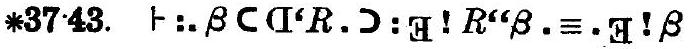
\includegraphics[max width=\textwidth, alt={}, center]{bc1848bf-39e8-4760-b069-9936044df683-163_49_688_1038_148}\\
Dem．\\
ト $\cdot * 37 \cdot 401 \cdot * 35 \cdot 65 \cdot$ つ $: . \mathrm{Hp} \cdot$ ɔ $: R^{\prime \prime} \beta=\mathrm{D}^{\prime}(R \uparrow \beta) \cdot \beta=\mathrm{G}^{\prime}(R \uparrow \beta)$（1） ト．（1）．＊33．24．วト．Prop\\
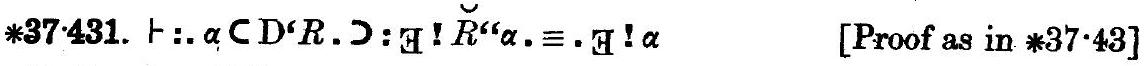
\includegraphics[max width=\textwidth, alt={}, center]{bc1848bf-39e8-4760-b069-9936044df683-163_66_1146_1231_148}\\
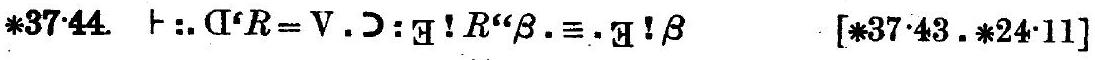
\includegraphics[max width=\textwidth, alt={}, center]{bc1848bf-39e8-4760-b069-9936044df683-163_60_1095_1293_148}\\
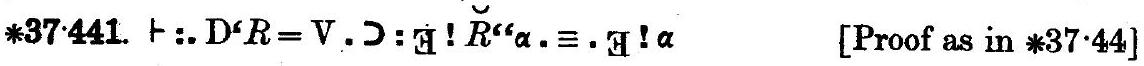
\includegraphics[max width=\textwidth, alt={}, center]{bc1848bf-39e8-4760-b069-9936044df683-163_66_1144_1347_148}\\
＊37．45．F：．（ $y$ ）．E！$R^{6} y$ ． ： H ！$R^{\prime \prime} \beta$ ．三 H ！$\beta$［＊33．431．＊37．43］\\
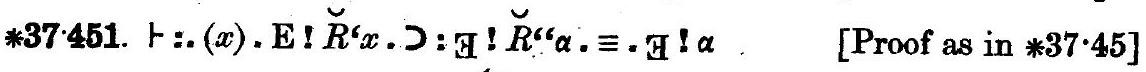
\includegraphics[max width=\textwidth, alt={}, center]{bc1848bf-39e8-4760-b069-9936044df683-163_72_1146_1459_148}\\
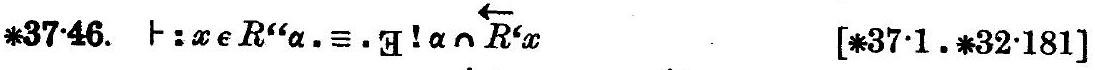
\includegraphics[max width=\textwidth, alt={}, center]{bc1848bf-39e8-4760-b069-9936044df683-163_70_1095_1524_148}\\
＊37．461． $\mathrm{F}: x \sim \epsilon \mathrm{R}^{\prime \prime} \alpha . \equiv \cdot \alpha \cap \overleftarrow{R}^{\prime} x=\Lambda . \equiv \overleftarrow{R}^{\prime} x \mathrm{C}-\alpha \quad$［＊37．46．＊24．311］\\
＊37．462． $\mathrm{F}: x \sim \epsilon \breve{R}^{\prime \prime} \alpha . \equiv \alpha \cap \vec{R}^{\prime} x=\Lambda . \equiv . \vec{R}^{\prime} x \mathrm{C}-\alpha \quad$［＊37．461．＊32．241］\\
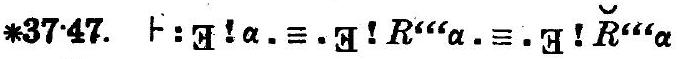
\includegraphics[max width=\textwidth, alt={}, center]{bc1848bf-39e8-4760-b069-9936044df683-163_59_679_1718_148}\\
Dem．


\begin{align*}
& \text { [(*37.04)] } \quad \equiv . \mathrm{H}!R \text { "α }  \tag{1}\\
& \text { ト. (1) } \frac{\breve{R}}{R} \text {. つト: } \frac{H!\alpha . \equiv \text { 月! } \breve{R}^{\prime \prime \prime} \alpha}{\alpha}  \tag{2}\\
& \text { ト.(1).(2). ɔ․ Prōp }
\end{align*}


＊37．5． 卜：$(\beta) \cdot P^{\prime \prime \prime} \beta=Q^{\prime} \beta \cdot \supset \cdot(\kappa) \cdot P$＂$\kappa=Q$＂$\kappa$\\
Dem．

$$
\begin{aligned}
& \text { ト. *37.12. ɔㅡ:Hp. ɔ. } P_{\mathrm{e}}=Q \text {. } \\
& \text { [*37-13] ɔ. } P_{e}{ }^{\prime \prime} \kappa=Q \text { " } \kappa \text {. } \\
& \text { [(*37.04)] ɔ.P"" } \kappa=Q \text { " } \kappa \text { : ว!.Prop }
\end{aligned}
$$

＊37：501．．F．$\beta \cap \mathbb{C}^{\prime} R \subset \breve{R}$＂$R$＂$\beta$\\
Dem．\\
ト ．＊37－1．＊10．24．ɔ ：$y \in \beta . x R y$. J．$x \in R^{\prime \prime} \beta:$\\
［Exp．＊10－11－21］ɔ ：$. y \in \beta . \supset: x R y . \nu_{x}: x \in R$＂$\beta:$\\
［＊4•7］$\supset: x R y . \partial_{x} . x R y . x \in R$＂$\beta$ ：\\
［＊10．28］ɔ：（Gx）．xRy．ɔ．（gx）．xRy．x $\in R^{\prime \prime \beta}$ ：\\
$[* 33 \cdot 131 \cdot * 37 \cdot 105] \quad \nu: y \in \mathbb{C}$ ⋅ $R . \supset . y \in R^{\prime \prime} R^{\prime \prime \beta}$

ト．（1）．Imp．＊22：33．ɔ


\begin{equation*}
\vdash: y \in \beta \cap \mathbb{C}^{\prime} R . \supset . y \in \breve{R} \text { " } R \text { " } \beta: \supset \vdash . \text { Prop } \tag{1}
\end{equation*}


＊37．502．r．$\alpha \cap \mathrm{D}$＂$R \subset R$＂$\breve{R}$＂$\alpha$［Similar proof］\\
＊37：51．$\quad \mathrm{f}: \beta \subset \mathrm{G}^{\prime} R . \equiv \beta \subset \breve{R}$＂$R$＂$\beta$\\
Dem．


\begin{align*}
& \text { ト } . * 37.501 . * 22.621 . \text { つ }: \beta \text { C } \text { I }^{\prime} R . \text { ɔ } . \beta \text { C } \breve{R} \text { " } R \text { " } \beta  \tag{1}\\
& \text { ト. } * 37 \text { ⋅ 16. } \quad \text { つ }: \beta \subset \breve{R} \text { " } R \text { " } \beta . \text { ɔ } . \beta \subset \text { T }^{\prime} R  \tag{2}\\
& \text { ト.(1).(2). ɔト.Prop }
\end{align*}


＊3752．$\quad \mathrm{f}: \alpha \subset \mathrm{D} \prime$ R．$\equiv \alpha \subset R$＂$\breve{R}$＂$\alpha$［Similar proof］\\
The following propositions，down to $* 37.7$ exclusive，are concerned with the special properties of $R$＂$\beta$ which result from the hypothesis E ！！$R$＂$\beta$ ，de－ fined in＊37．05．The hypothesis E ！！$R$＂$\beta$ is important，because it has many consequences and is satisfied in many cases with which we wish to deal．\\
＊376． ト： $\mathrm{E} \|$ ！$R^{\prime \prime} \beta$ ．$\supset . R^{\prime \prime} \beta=\widehat{x}\left\{(\right.$ H $\left.y) . y \in \beta . x=R^{\prime} y\right\}$\\
This proposition is very important，and is used constantly．\\
Dem．\\
ト．$* 37$ ⋅ 104. ɔ $:: \mathrm{Hp}$. J ：$y \in \beta$. J $_{y}: \mathrm{E}!R^{\prime} y:$\\
［＊30．4］\\
$\nu_{y}: x=R^{6} y . \equiv x R y:$.\\
［＊5＊32］\\
ɔ ：．$y \in \beta . x=R^{6} y . \equiv_{y} . y \in \beta . x R y$ ：．\\
［＊10．281］\\
J：．（आ $y$ ）$y \in \beta . x=R^{6} y . \equiv .($ H $y) . y \in \beta . x R y$ ．\\
［＊37•1］


\begin{equation*}
\equiv x \in R^{\prime \prime} \beta \tag{1}
\end{equation*}


ト．（1）．＊10．11．21．＊2033．ɔ…Prop\\
＊37．601． $\mathrm{F}:(x) . \mathrm{E}!R^{\prime} x . \supset . R^{\prime \prime} \mathrm{V}=\widehat{x}\left\{(\mathrm{H} y) . x=R^{\prime} y\right\}$\\
Dem．\\
ト．＊2：02．＊10．11．27．ɔ ：．Hp．ɔ ：$x \in \mathrm{~V} . \partial_{x} . \mathrm{E}!R^{\prime} x:$

\begin{verbatim}
[*37•104] つ: E ! ! R"V:
[*37.6] $\supset: R^{\prime \prime} \mathrm{V}=\widehat{x}\left\{(\mathrm{~g} y) . y \in \mathrm{~V} . x=R^{\prime} y\right\}$
ト. *24:104. *4:73. ɔㅐ: $y \in \mathrm{~V} . x=R^{6} y . \equiv . x=R^{6} y$ :
[*10•11•281] $\quad \supset \vdash:(\mathrm{H} y) \cdot y \in \mathrm{~V} \cdot x=R^{6} y \cdot \equiv \cdot(\mathrm{H} y) \cdot x=R^{6} y:$
[*20•15] $\quad \supset \vdash: \widehat{x}\left\{(\mathrm{H} y) \cdot y \in \mathrm{~V} \cdot x=R^{\prime} y\right\}=\widehat{x}\left\{(\mathrm{G} y) \cdot x=R^{\prime} y\right\}$
ト.(1).(2). ɔト.Prop
\end{verbatim}

\section*{＊37．61．$+:: \mathrm{E}!!R^{\prime \prime} \beta$. J：．$R^{\prime \prime} \beta$ C $\alpha . \equiv: y \in \beta . \partial_{y} . R^{\prime} y \in \alpha$}
Dem．


\begin{align*}
& \text { ト.*3717. ɔト:: } R \text { " } \beta \text { C } \alpha . \equiv: y \in \beta . x R y . \mathcal{J}_{x, y}, x \in \alpha: . \\
& \text { [*11•2•62] } \quad \equiv: . y \in \beta . \nu_{y}: x R y . \nu_{x} . x \in \alpha  \tag{1}\\
& \text { ト. *37.104. ɔ ::: Hp. ɔ:: } y \in \beta . \partial_{y}: . \mathrm{E}!R^{6} y: . \\
& \text { [*30.33] } \quad \nu_{y}: R^{\prime} y \in \alpha . \equiv: x R y . \nu_{x} . x \in \alpha  \tag{2}\\
& \text { ト.(1).(2). } \supset \vdash:: \mathrm{Hp} . \supset: R^{\prime \prime} \beta \subset \alpha . \equiv: y \in \beta . \partial_{y} . R^{\prime} y \in \alpha:: \supset \text {. Prop }
\end{align*}


＊37．62．$\vdash: \mathrm{E}!R^{\prime} y, y \in \alpha . \supset . R^{\prime} y \in R^{\prime \prime} \alpha$\\
Dem．


\begin{align*}
& \text { ト.*30:33.ɔ } \\
& \text { ト:: } \mathrm{E}!R^{6} y . \text { J: } R^{6} y \in R^{6 \prime} \alpha . \equiv: x R y . \partial_{x} . x \in R^{\prime \prime} \alpha  \tag{1}\\
& \text { ト.*32. ɔト:. } y \in \alpha \text {. } \supset: x R y \text {. ɔ. } y \in \alpha \text {. } x R y \text {. } \\
& \text { [*10.24.*37.1] J.xtR"α }  \tag{2}\\
& \text { ト.(2).*10.11-21. ɔㅇ: } y \in \alpha \text {. } \text { ɔ }: x R y \text {. } J_{x} . x \in R \text { " } \alpha  \tag{3}\\
& \text { ト. (1). (3). ɔト.Prop }
\end{align*}


The above is the type of inference concerning which Jevons says＊： ＂I remember the late Prof．De Morgan remarking that all Aristotle＇s logic could not prove that＇Because a horse is an animal，the head of a horse is the head of an animal．＇＂It must be confessed that this was a merit in Aristotle＇s logic，since the proposed inference is fallacious without the added premiss＂E ！the head of the horse in question．＂E．g．it does not hold for an oyster or a hydra．But with the addition $\mathrm{E}!R^{6} y$ ，the above proposition gives an important and common type of asyllogistic inference．\\
＊37．63．$\vdash:: \mathrm{E}!!R^{\prime \prime} \alpha$. J：．$x \in R^{\prime \prime} \alpha . \partial_{x}, \psi x: \equiv: y \in \alpha . \partial_{y} . \psi\left(R^{\prime} y\right)$\\
Dem．


\begin{align*}
& \text { ト. *37.1. ɔト:: } x \in R \text { " } \alpha . \partial_{x} . \psi x: \equiv:(\text { H } y) . y \in \alpha . x R y . \partial_{x} . \psi x: . \\
& \text { [*10.23] } \equiv: . y \in \alpha . x R y . \partial_{x, y} . \psi x: . \\
& \text { [*11.262] } \equiv: . y \in \alpha . \partial_{y}: x R y . \partial_{x} . \psi x  \tag{1}\\
& \text { ト . } * 37 \text { ⋅ } 104 . \text { ɔ }:: . \mathrm{Hp} . \text { J:: } y \in \alpha . \text { J }_{y}: . \mathrm{E}!R^{6} y: . \\
& \text { [*30.33] } \quad \nu_{y}: . \psi\left(R^{6} y\right) . \equiv: x R y . \nu_{x} . \psi x  \tag{2}\\
& \text { ト.(1).(2).ɔ } . \text { Prop }
\end{align*}


This proposition is very frequently used．

\footnotetext{${ }^{*}$ Principles of Science，chap．1．（p． 18 of edition of 1887）．
}
＊37．64．$\vdash: . \mathrm{E}!!R^{\prime \prime} \alpha . \supset:(\mathrm{H} y) . y \in \alpha . \psi\left(R^{\prime} y\right) . \equiv .(\mathrm{H} x) . x \in R^{\prime \prime} \alpha . \psi x$\\
Dem．\\
ト．$* 3033$. ɔ $:: \mathrm{Hp}$. ɔ ：$y \in \alpha$. つ $: \psi\left(R^{6} y\right) . \equiv($ H $x) . x R y . \psi x:$.\\
［＊5＊32］

\begin{equation*}
\text { כ :. } y \in \alpha \cdot \psi\left(R^{\prime} y\right) \cdot \equiv: y \in \alpha:\left(\mathrm{H}^{x}\right) \cdot x R y \cdot \psi x \tag{1}
\end{equation*}


ト．（1）．＊10．11．21．281．J\\
।：：Нр．ɔ：（आ $y$ ）．$y \in \alpha \cdot \psi\left(R^{6} y\right) \cdot \equiv:(\mathrm{H} y): y \in \alpha:(\mathrm{H} x) \cdot x R y \cdot \psi x:$\\
［＊11•6］$\equiv:\left(\mathrm{H}^{x}\right):(\mathrm{H} y) . y \in \alpha . x R y: \psi x:$\\
［＊37•1］

$$
\equiv:\left(G^{x}\right) \cdot x \in R^{\prime \prime} \alpha \cdot \psi x:: \supset \vdash . \text { Prop }
$$

＊3765．$+: E!!R$＂$\beta . \alpha \subset R$＂$\beta . \supset . \alpha=R$＂$(\breve{R}$＂$\alpha \cap \beta)$

\section*{Dem．}
ト．＊3021．＊3．27．ɔ ：：Hp．ɔ：$y \in \beta . \supset_{y}: z R y . x R y . \supset . z=x$

ト．＊37．1．つト：．Hp．ɔ：


\begin{equation*}
x \in R \text { " }(\breve{R} \text { " } \alpha \cap \beta) \cdot \equiv(\mathrm{H} y) \cdot y \in \breve{R} \text { " } \alpha \cap \beta \cdot x R y . \tag{1}
\end{equation*}


［＊37•105．＊11．55］

$$
\equiv \cdot(G y, z), z \in \alpha, z R y, y \in \beta, x R y .
$$

［（1）．＊4＇71］ $\equiv .(\mathrm{H} y, z) . z \in \alpha . z R y . y \in \beta . x R y . z=x$.\\
［＊13•194］

$$
\equiv \cdot(\text { H } y, z) \cdot z \in \alpha \cdot y \in \beta \cdot x R y \cdot z=x .
$$

［＊13•195］

$$
\equiv(\text { 马 } y), x \in \alpha, y \in \beta, x R y .
$$

［＊10：35．＊37．1］

$$
\equiv . x \in \alpha . x \in R \text { " } \beta .
$$

［＊4．71．Hp］

$$
\equiv . x \in \alpha: . \supset \vdash . \text { Prop }
$$

＊37．66． ト：． $\mathrm{E}!!R^{\prime \prime} \beta . \supset: \alpha \subset R^{\prime \prime} \beta . \equiv .(\mathrm{H} \gamma) \cdot \gamma \subset \beta . \alpha=R^{\prime \prime} \gamma$\\
Dem．\\
ト．＊37．65．Exp．＊13195．＊2243．つ


\begin{equation*}
\vdash: \text { Hp } . \supset: \alpha \subset R^{\prime \prime} \beta . \supset \cdot(\text { H } \gamma) \cdot \gamma \subset \beta \cdot \alpha=R^{\prime \prime} \gamma \tag{1}
\end{equation*}


ㅏ．$* 37 \cdot 2 . * 13 \cdot 13$. ɔ $: \gamma$ C $\beta . \alpha=R^{\prime \prime} \gamma$. ɔ.$\alpha$ C $R^{\prime \prime} \beta$ ：


\begin{equation*}
[* 10 \cdot 11 \cdot 23] \quad \supset \vee:(H \gamma) \cdot \gamma \subset \beta \cdot \alpha=R^{\prime \prime} \gamma \cdot \supset \cdot \alpha \subset R^{\prime \prime} \beta \tag{2}
\end{equation*}


ト．（1）．（2）．ɔ।．Prop\\
＊37．67．$\vdash:, z \in \gamma \cdot \partial_{z} \cdot \mathrm{E}!R^{\prime} S^{\prime} z: \partial \cdot R^{\prime \prime} S^{\prime \prime} \gamma=\widehat{x}\left\{\left(\mathrm{H}^{z}\right) \cdot z \in \gamma \cdot x=R^{\prime} S^{\prime} z\right\}$ Dem．


\begin{equation*}
\text { ト } \cdot * 34 \cdot 41 \text {. } \quad \supset \vdash: \mathrm{Hp} \cdot z \in \gamma \cdot \partial_{z} \cdot R^{6} S^{6} z=(R \mid S)^{6} z \tag{1}
\end{equation*}


ト．（1）．$* 1421$. J $: \mathrm{Hp} . z \in \gamma . \mathcal{J}_{z} . \mathrm{E}!(R \mid S)^{6} z$

ト．（2）．＊37．6．ɔㅐ：Hp．ɔ．$(R \mid S)^{6 \prime} \gamma=\widehat{x}\left\{\left(\mathrm{H}^{z}\right) \cdot z \in \gamma \cdot \bar{x}=(R \mid S)^{6} \gamma\right\}$\\
［（1）］


\begin{equation*}
=\hat{x}\left\{\left(H^{z} z\right) \cdot z \in \gamma \cdot x=R^{6} S^{6} \gamma\right\} \tag{2}
\end{equation*}


ト．＊37．33．$\quad$ ɔ $. R^{\prime \prime} S^{\prime \prime} \gamma=(R \mid S)^{\prime \prime} \gamma$

ト．（3）．（4）．ɔト．Prop

\section*{＊37．68． ！$: z \in \gamma \cdot \partial_{z} \cdot P^{\prime} Q^{\prime} z=R^{\prime} z: \supset \cdot P^{\prime \prime} Q^{\prime \prime} \gamma=R^{\prime \prime} \gamma$}
Dem．\\
ト．$* 1421$. つ $:$ Hp.$z \in \gamma$. J．E $!P^{6} Q^{6} z . \mathrm{E}!R^{6} z$.\\
［＊34．41］\\
J．$P^{6} Q^{6} z=(P \mid Q)^{6} z . \mathrm{E}!R^{6} z$ ．\\
［ $* 14 \cdot 21 \cdot 131 \cdot 144 . \mathrm{Hp}$ ］\\
J．E！$(P \mid Q)^{6} z \cdot(P \mid Q)^{6} z=R^{6} z$


\begin{align*}
& \vdash \cdot * 37 \cdot 33 \cdot \supset \vdash \cdot P " Q " \gamma=(P \mid Q)^{\prime \prime} \gamma  \tag{3}\\
& \vdash \cdot(2) \cdot(3) \cdot * 37 \cdot 6 \cdot \supset \\
& \vdash: H p \cdot \supset \cdot P^{\prime \prime} Q " \gamma=\widehat{x}\left\{(\vec{H} z) \cdot z \in \gamma \cdot x=(P \mid Q)^{\prime} z\right\} \\
& \begin{array}{ll}
{[(2)]} & =\widehat{x}\left\{\left(\text { (Hz) } \cdot z \in \gamma \cdot x=R^{\prime} z\right\}\right. \\
{[* 37 \cdot 6 \cdot(1)] \quad} & =R^{\prime \prime} z: \supset \vdash . \text { Prop }
\end{array}
\end{align*}


＊37．69．F：．$y \in \beta$ ．$\partial_{y} \cdot R^{\prime} y=S^{\prime} y: \partial \cdot R^{\prime \prime} \beta=S^{\prime \prime} \beta$\\
Dem．


\begin{align*}
& \text { ト. } * 14.21 \text {. } \text { J }:: \text { Hp. } \text { J:. } y \in \beta \text {. } \text {. E }!R^{6} y \text {. E }!S^{6} y \text { :. }  \tag{1}\\
& \text { [*304] } \quad \supset: . y \in \beta . \supset: x R y . \equiv . x=R^{6} y \text {. } \\
& \text { [*14•142] } \quad \equiv . x=S^{6} y \text {. } \\
& \text { [*30•4.(1)] } \quad \equiv . x S y: . \\
& \text { [*5.32] } \quad \text { J: } y \in \beta . x R y . \equiv . y \in \beta . x S y  \tag{2}\\
& \text { ト.(2).*10.11.21.281. ɔ } \\
& \text { । :. Hp. ɔ : (H } y \text { ). } y \in \beta . x R y . \equiv .(\text { H } y) . y \in \beta . x S y \text { : } \\
& {[* 37 \cdot 1] \nu: x \in R \text { " } \beta . \equiv . x \in S \text { " } \beta: . \supset \vdash \text {. Prop }}
\end{align*}


A specially important case of $R$＂$\beta$ is $\vec{R}$＂$\beta$ or $\overleftarrow{R}$＂$\beta$ ．This case will be further studied later（in $* 70$ ）；for the present，we shall only give a few preliminary propositions about it．It will be observed that the hypothesis $\mathrm{E}!!\vec{R}$＂$\beta$ or $\mathrm{E}!!\overleftarrow{R}$＂$\beta$ is always verified，in virtue of $* 32 \cdot 12 \cdot 121$ ．Hence the following applications of $* 37.6$ ff．：

\begin{center}
\begin{tabular}{|l|l|l|}
\hline
 & ＊377．$\quad \vdash . \vec{R}^{\prime \prime} \beta=\hat{\alpha}\{($ H $y) \cdot y \in \beta \cdot \alpha=\vec{R} y\}$ & ［＊37．6．＊32．12］ \\
\hline
＊37701． & ＋．$\overleftarrow{R^{\prime \prime}} \alpha=\hat{\beta}\left\{\left(\Psi^{\prime} x\right) \cdot x \in \alpha \cdot \beta=\overleftarrow{R}^{\prime} x\right\}$ & ［＊37．6．＊32．121］ \\
\hline
＊37．702． & ト $: \vec{R}^{\prime \prime} \beta \subset_{\kappa} . \equiv: y \in \beta . \partial_{y} . \vec{R}^{\prime} y \in \kappa$ & ［＊37．61］ \\
\hline
＊37703． & ＋$: \overleftarrow{R^{\prime \prime}} \beta \subset \kappa . \equiv: x \in \beta . \supset_{x}, \overleftarrow{R^{\prime}} x \in \kappa$ & ［＊37．61］ \\
\hline
＊37704． & t：$y \in \alpha . \supset . \vec{R}^{\prime} y \in \vec{R}^{\prime \prime} \alpha$ & ［＊37．62．＊32．12］ \\
\hline
＊37．705． & ト：$x \in \alpha$ ． J．$\overleftarrow{R}^{\prime} x \in \overleftarrow{R}^{\prime \prime} \alpha$ & ［＊37．62．＊32．121］ \\
\hline
＊37．706． & $\vdash:, \alpha \in \vec{R}$＂$\beta . \partial_{a} \cdot \psi \alpha: \equiv: y \in \beta \cdot \nu_{y} \cdot \psi\left(\vec{R}^{\prime} y\right)$ & ［＊37．63］ \\
\hline
＊37707． & $\vdash:, \beta \in \overleftarrow{R}^{\prime \prime} \alpha \cdot \nu_{\beta} \cdot \psi \beta: \equiv: x \in \alpha \cdot \nu_{x} \cdot \psi\left(\overleftarrow{R^{\prime}} x\right)$ & ［＊37．63］ \\
\hline
＊37．708． & ト：$\left(\right.$ H $\left.^{\alpha}\right) \cdot \alpha \in \vec{R}$＂$\beta \cdot \psi \alpha . \equiv .($ H $y) \cdot y \in \beta \cdot \psi(\vec{R}$ ⋅ $y)$ & ［＊37．64］ \\
\hline
＊37．709． & ト：．$\left(\mathrm{H}^{\alpha}\right) \cdot \alpha \in \overleftarrow{R}{ }^{\prime \prime} \beta \cdot \psi \alpha \cdot \equiv \cdot\left(\mathrm{H}^{\prime} x\right) \cdot x \in \beta \cdot \psi\left(\overleftarrow{R}^{\prime} x\right)$ & ［＊37．64］ \\
\hline
$* 37.71$ ． & ㅏ：$\kappa \subset \overrightarrow{R^{\prime \prime}} \beta . \supset . \kappa=\overrightarrow{R^{\prime \prime}}\left\{\left(\mathrm{Cnv}^{\prime} \vec{R}\right)^{\prime \prime} \kappa \cap \beta\right\}$ & ［＊37．65］ \\
\hline
＊37711． & 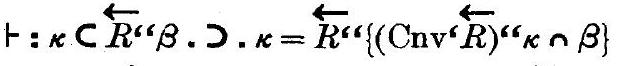
\includegraphics[max width=\textwidth, alt={}]{bc1848bf-39e8-4760-b069-9936044df683-167_66_618_1883_293}
 & ［＊37．65］ \\
\hline
＊37712． & ト：$\kappa \subset \overrightarrow{R^{\prime \prime}} \beta . \equiv($ H $\gamma) \cdot \gamma \subset \beta \cdot \kappa=\overrightarrow{R^{\prime \prime}} \gamma$ & ［＊37．66］ \\
\hline
＊37．713． & $\mathrm{F}: \kappa \subset \overleftarrow{R} \prime \beta \cdot \equiv(\mathrm{G} \gamma) \cdot \gamma \subset \beta \cdot \kappa=\overleftarrow{R^{\prime \prime} \gamma}$ & ［＊37．66］ \\
\hline
\end{tabular}
\end{center}

＊37．72．$\vdash: R=P \mid Q . \supset . \vec{R}$＂$\gamma=P$＂$\vec{Q}$＂$\gamma$\\
Dem．

$$
\begin{aligned}
& \text { ト . *37-11 302. ɔ : Hp. ɔ . ( } z \text { ) . } P_{\epsilon}^{\prime} \vec{Q}^{\prime} z=\vec{R}^{\prime} z \text {. } \\
& \text { [*37.68] } \\
& \text { ɔ. } P_{\epsilon} \text { " } \vec{Q} \text { " } \gamma=\vec{R} \text { " } \gamma \text {. } \\
& \text { [(*37•04)] } \\
& \text { ɔ. P""Q"‘ } \gamma=\vec{R} \text { " } \gamma \text { : ɔト. Prop }
\end{aligned}
$$

＊37．721．$\vdash: R=P \mid Q . \supset . \overleftarrow{R} \prime \prime \gamma=\breve{Q}$＂$\overleftarrow{P}$＂$\gamma \quad$［Proof as in＊37．72］\\
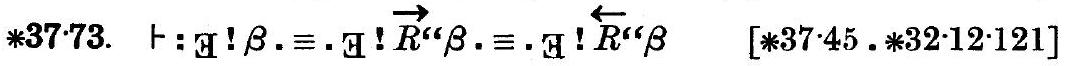
\includegraphics[max width=\textwidth, alt={}, center]{bc1848bf-39e8-4760-b069-9936044df683-168_66_1066_566_222}\\
＊37．731． ！$: \beta=\Lambda . \equiv . \vec{R}^{\prime \prime} \beta=\Lambda . \equiv . \overleftarrow{R} \prime \beta=\Lambda \quad$［＊37．73．Transp］\\
Observe that the $\Lambda$＇s which occur in this proposition will not be all of the same type．E．g．if $R$ relates individuals to individuals，the first $\Lambda$ will be the class of no individuals，while the second and third will be the class of no classes．Thus the ambiguity which attaches to the type of $\Lambda$ must be differently determined for different occurrences of $\Lambda$ in this proposition．In general，when this is the case with our ambiguous symbols，we shall adopt a notation which indicates the fact．But when the ambiguous symbol is $\Lambda$ ，it seems hardly worth while．\\
＊37．74．$+: \beta \subset \mathbb{C}$ ⋅ $R . \equiv: \alpha \in \vec{R}$＂$\beta . \nu_{a} \cdot$ A！$\alpha$\\
Dem．

$$
\begin{aligned}
\vdash \cdot * 37 \cdot 706 \cdot \supset \vdash: \alpha \in \vec{R} \prime \beta \cdot \supset_{a} \cdot \mathcal{H}!\alpha: & \equiv: y \in \beta \cdot \supset_{y} \cdot \mathcal{H}!\vec{R}^{\prime} y: \\
& \equiv: \beta \subset G^{\prime} R: . \supset \text {. Prop } \\
{[* 33 \cdot 31] } & \\
&
\end{aligned}
$$

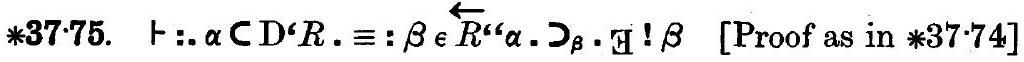
\includegraphics[max width=\textwidth, alt={}, center]{bc1848bf-39e8-4760-b069-9936044df683-168_62_1024_1249_220}\\
＊37．76．$\quad$ ト.$\vec{R}$＂$\beta \subset \mathrm{Cls}$\\
Dem．

$$
\begin{array}{ll}
\vdash \cdot * 37 \cdot 7 \cdot \supset \vdash: \alpha \in \overrightarrow{R^{\prime}} \beta \cdot \beta:(\mathrm{H} y) \cdot y \in \beta \cdot \alpha=\overrightarrow{R^{\prime}} y: \\
{[* 10 \cdot 5]} & \supset:(\mathrm{H} y) \cdot \alpha=\overrightarrow{R^{\prime}} y: \\
{[* 32 \cdot 13]} & \supset:(\mathrm{H} y) \cdot \alpha=\widehat{x}(x R y): \\
{[* 20 \cdot 16]} & \supset:(\mathrm{H} \phi) \cdot \alpha=\widehat{x}(\phi!x): \\
{[* 20 \cdot 4]} & \supset: \alpha \in \mathrm{Cls}: \text { J } . \text { Prop }
\end{array}
$$

＊37．761．.$+ \overleftarrow{R}$＂$\alpha \mathrm{C} \mathrm{Cls}$\\
［Proof as in＊37．76］\\
＊37．77． $\mathrm{F}: \alpha \in \vec{R}$＂ $\mathrm{U}^{\prime} R . \partial_{a}$. H！$\alpha \quad$［＊37．74．＊22．42］\\
＊37．771． $\mathrm{F}: \beta \in \overleftarrow{R} ‘ \mathrm{C} ‘$ ⋅ $R . \partial_{\beta} . \mathrm{H}!\beta \quad$［Proof as in＊37．77］\\
＊37．772． $\mathrm{F} . \Lambda \sim \epsilon \vec{R}^{\prime \prime} \mathbb{G}^{\prime} R \quad$［＊37．77．＊24．63］\\
＊37－773．.$+ \Lambda \sim \epsilon \overleftarrow{R}^{\prime \prime} \mathrm{D}^{\prime} R$\\
［＊37．771．＊24．63］\\
＊37．78． ト $. \mathrm{D} \wedge \vec{R}=\overrightarrow{R^{\prime}}$ ‘ V\\
［＊37•28］\\
*37.781. ト . $\mathrm{D} \overleftarrow{R}=\overleftarrow{R} \prime \mathrm{~V}$ [*37.28]\\
*37.79. $+. \vec{R}^{\prime \prime} \mathrm{V}=\hat{\alpha}\left\{(\mathrm{H} y) . \alpha=\vec{R}^{\prime} y\right\} \quad[* 37.601 . * 32 \cdot 12]$\\
*37•791. $+. \overleftarrow{R^{\prime \prime}} \mathrm{V}=\hat{\beta}\left\{\left(\mathrm{I}^{x} x\right) \cdot \beta=\overleftarrow{R^{\prime}} x\right\} \quad[* 37 \cdot 601 \cdot * 32 \cdot 121]$\\
*378. $\quad$ ト. $(\alpha \uparrow \beta) \mid S=\alpha \uparrow \breve{S} \prime \beta$\\
Dem.\\
$\vdash . * 35 \cdot 103 . * 34 \cdot 1$. J $: x\{(\alpha \uparrow \beta) \mid S\} z . \equiv .($ H $y) . x \in \alpha . y \in \beta . y S z$.\\[0pt]
[\textit{10}35**37•105]\\
$\equiv x \in \alpha . z \in \breve{S} \| \beta$.\\[0pt]
[*35•103]\\
$\equiv . x(\alpha \uparrow \breve{S}$ " $\beta) z:$ ɔ. Prop\\
*37.81. $\quad$. $R \mid(\alpha \uparrow \beta)=\left(R^{\prime \prime} \alpha\right) \uparrow \beta$\\[0pt]
[Proof as in *37:8]\\
*37.82. * . $R|(\dot{\alpha} \uparrow \beta)| S=(R$ " $\alpha) \uparrow(\breve{S}$ " $\beta)$\\[0pt]
[*37.8.81]

\section*{*38. RELATIONS AND CLASSES DERIVED FROM A DOUBLE DESCRIPTIVE FUNCTION}
\section*{Summary of $* 38$.}
A double descriptive function is a non-propositional function of two arguments, such as $\alpha \cap \beta, \alpha \cup \beta, R \cap S, R \cup S, R \mid S, \alpha \upharpoonleft R, R \upharpoonright \alpha, R\lceil\alpha$. The propositions of the present number apply to all such functions, assuming the notation to be (as in the above instances) a functional sign placed between the two arguments. In order to deal with all analogous cases at once, we shall in this number adopt the notation

$$
x \neq y,
$$

where " $\boldsymbol{q}$ " stands for any such sign as $\cap, \cup, \dot{\wedge}, \mho, \mid, 1, \upharpoonright$, or any functional sign to be hereafter defined and satisfying the condition

$$
(x, y) . \mathrm{E}!(x \neq y) .
$$

The derived relations and classes with which we shall be concerned may be illustrated by taking the case of $\alpha \cap \beta$. The relation of $\alpha \cap \beta$ to $\beta$ will be written $\alpha \cap$, and the relation of $\alpha \cap \beta$ to $\alpha$ will be written $\cap \beta$. Thus we shall have

$$
\text { F. } \alpha \cap \beta=\alpha \cap \cap^{\prime} \beta=\cap \beta^{\prime} \alpha .
$$

The utility of this notation is chiefly due to the possibility of such notations as $\alpha \cap^{6} \kappa$ and $\cap \beta^{6 \prime} \kappa$. For example, take such a phrase as "the foreign members of English Clubs." Then if we put $\alpha=$ foreigners, $\kappa=$ English Clubs, we have

$$
\alpha \cap \text { " } \kappa=\text { the classes of foreign members of the various English Clubs. }
$$

Or again, let $\alpha$ be a conic, and $\kappa$ a pencil of lines; then

$$
\alpha \cap \text { " } \kappa=\text { the various pairs of points in which members of } \kappa \text { meet } \alpha .
$$

In this case, since $\alpha \cap \beta=\beta \cap \alpha$, we have $\alpha \cap=\cap \alpha$. But when the function concerned is not commutative, this does not hold. Thus for example we do not have $R|=| R$.

The notations of this number will be frequently applied hereafter to $R \mid S$. In accordance with what was said above, we write $R \mid$ for the relation of $R \mid S$ to $S$, and $\mid S$ for the relation of $R \mid S$ to $R$. Hence we have

$$
\left.R\right|^{\prime} S=\left|S^{\prime} R=R\right| S .
$$

Hence $\mid S^{\prime \prime} \lambda$ will be the class of relations obtained by taking members of $\lambda$ and relatively multiplying them by $S$. Thus if $\lambda$ were the class of relations first cousin, second cousin, etc., and $S$ were the relation of parent to child, | $S$ " $\lambda$ would be the class of relations first cousin once removed, second cousin once removed, etc., taken in the sense which goes from the older to the younger generation.

It is often convenient to be able to exhibit | $S^{\prime \prime} \lambda$ and kindred expressions as descriptive functions of the first argument instead of the second. For this purpose we put

$$
\lambda|, S=| S^{6 \prime} \lambda
$$

with similar notations for other descriptive double functions. We then have, just as in the case of $R \mid S$,

$$
\left.\lambda\right|_{,,} S=,, S^{\prime} \lambda=\lambda \mid, S .
$$

This enables us to form the class $\lambda$,, " $\mu$. This class is chiefly useful because the members of its members (i.e. $s^{\prime} \lambda \mid, " \mu$, as we shall define it in $* 40$ ) constitute the class of all products $R \mid S$ that can be formed of a member of $\lambda$ and a member of $\mu$.

Thus we are led to three general definitions for descriptive double functions, namely (if $x \& y$ be any such function)\\
$x \neq$ is the relation of $x \neq y$ to $y$ for any $y$,\\
\& $y$,, " ,, " „ $x$ „ $x$,\\
$\alpha, y$ is the class of values of $x \neq y$ when $x$ is an $\alpha$.\\
Since $\alpha, y$ is again a descriptive double function, the first two of the above definitions can be applied to it. The third definition, for typographical reasons, cannot be applied conveniently, though theoretically it is of course applicable. The relations $x \neq$ and $\& y$ represent the general idea contained in some of the uses in mathematics of the term "operation," e.g. +1 is the operation of adding 1 .

The uses of the notations introduced in the present number occur chiefly in arithmetic (Parts III and IV). Few propositions can be given at this stage, since most of the important uses of the notation here introduced depend upon the substitution of some special function for the general function " $f$ " here used. In the present number, the propositions given are all immediate consequences of the definitions.\\
*38.01.

$$
\begin{aligned}
& x \neq \widehat{u} \hat{y}(u=x \neq y) \quad \text { Df } \\
& \text { *38.02. } \quad \dot{q} y=\hat{u} \hat{x}(u=x \neq y) \quad \text { Df } \\
& \text { *38.03. } \quad \alpha \frac{\&}{,,} y=\mp y^{" \alpha} \quad \text { Df } \\
& \text { *38.1. } F_{:} u(x \neq) y . \equiv u=x \neq y \quad \text { [(*38.01)] } \\
& \text { *38.101. } \vdash: u(q y) x . \equiv . u=x \neq y \quad \text { [(*38.02)] } \\
& \text { *3811. F. } x \text { \& } y=\text { \& } y^{\prime} x=x \text { \& } y \text { [*381•101.*30.3] } \\
& \text { *3812. } \mathrm{F} . \mathrm{E}!x q^{6} y . \mathrm{E}!\neq y^{6} x \text { [*38.11.*14.21] } \\
& \text { *38.13. } F: u \in x \text { \& " } \alpha . \equiv \text {. (马 } y \text { ). } y \in \alpha . u=x \& y \quad \text { [*38.1.*37.1] } \\
& \text { *38131. } \vdash: u \in \ddagger y \text { " } a . \equiv .(\neg x) . x \in \alpha . u=x \neq y \quad[* 38.101 . * 37 \cdot 1]
\end{aligned}
$$

＊38．2．F．$\alpha \underset{,}{f} y=\& y^{\prime \prime} \alpha$［（＊38．03）］\\
＊38．21．F．$\alpha, \underset{,}{q} y=\hat{u}\left\{\left(\mathrm{H}^{x}\right) . x \in \alpha . u=x \neq y\right\} \quad[* 38.2 \cdot 131]$\\
＊38．22． ト．$\alpha_{,,}^{q} y=\underset{,, y^{\prime}}{q^{\prime}} \alpha=\alpha \underset{,,}{q} y$［＊38．11］\\
＊38．23．F．E！α σϕy．E！σ，y ${ }^{6} \alpha$［＊38．22．＊14．21］\\
＊3824．$F:$ G！$\alpha, y . \equiv$ ，$y$ ！$\alpha$\\
Dem．


\begin{align*}
& \vdash . * 38.21 \text {. } \supset \vdash: x \in \alpha . \supset .(x \neq y) \in \alpha \neq y \text {. }  \tag{1}\\
& \text { [*10.24] ɔ.ु!α,ο y }  \tag{2}\\
& \text { ト.(1).(2). ɔ } . \text { Prop }
\end{align*}


＊38．3．$\vdash . \alpha \neq$, ＂$\beta=\hat{\gamma}\{(\mathrm{H} y) \cdot y \in \beta \cdot \gamma=\alpha \underset{,,}{q} y\}=\hat{\gamma}\{(\mathrm{H} y) \cdot y \in \beta \cdot \gamma=\mp y$＂$\alpha\}$ ［＊38．13．2］\\
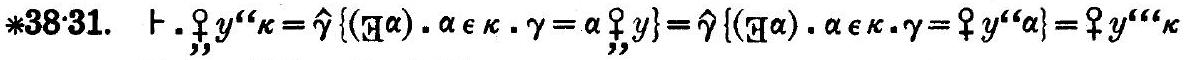
\includegraphics[max width=\textwidth, alt={}]{bc1848bf-39e8-4760-b069-9936044df683-172_60_1186_885_218} ［ $* 38 \cdot 131 \cdot 2 \cdot * 37 \cdot 103]$

\begin{itemize}
  \item 
\end{itemize}

\begin{itemize}
  \item 
\end{itemize}

\begin{itemize}
  \item 
\end{itemize}


\end{document}